%%%%%%%%%%%%%%%%%%%% book.tex %%%%%%%%%%%%%%%%%%%%%%%%%%%%%
%
% sample root file for the chapters of your "monograph"
%
% Use this file as a template for your own input.
%
%%%%%%%%%%%%%%%% Springer-Verlag %%%%%%%%%%%%%%%%%%%%%%%%%%


% RECOMMENDED %%%%%%%%%%%%%%%%%%%%%%%%%%%%%%%%%%%%%%%%%%%%%%%%%%%
% \documentclass[graybox,envcountchap,sectrefs]{xourse}
\documentclass{xourse}

% choose options for [] as required from the list
% in the Reference Guide

%\usepackage{mathptmx}
%\usepackage{helvet}
%\usepackage{courier}
%

%\usepackage{type1cm}         
%
%\usepackage{makeidx}         % allows index generation
%\usepackage{graphicx}        % standard LaTeX graphics tool
%                             % when including figure files
%\usepackage{multicol}        % used for the two-column index
%\usepackage[bottom]{footmisc}% places footnotes at page bottom
%
%\usepackage{newtxtext}       % 
%\usepackage[varvw]{newtxmath}       % selects Times Roman as basic font
%
%\usepackage{listings}
%\usepackage{xcolor}
%\usepackage{float}
%
%\definecolor{codegreen}{rgb}{0,0.6,0}
%\definecolor{codegray}{rgb}{0.5,0.5,0.5}
%\definecolor{codepurple}{rgb}{0.58,0,0.82}
%\definecolor{backcolour}{rgb}{0.95,0.95,0.92}

%\lstdefinestyle{mystyle}{
%    backgroundcolor=\color{backcolour},   
%    commentstyle=\color{codegreen},
%    keywordstyle=\color{magenta},
%    numberstyle=\tiny\color{codegray},
%    stringstyle=\color{codepurple},
%    basicstyle=\ttfamily\footnotesize,
%    breakatwhitespace=false,         
%    breaklines=true,                 
%    captionpos=b,                    
%    keepspaces=true,                 
%    numbers=left,                    
%    numbersep=5pt,                  
%    showspaces=false,                
%    showstringspaces=false,
%    showtabs=false,                  
%    tabsize=2
%}
%
%\lstset{style=mystyle}
%
%
%% see the list of further useful packages
%% in the Reference Guide
%
%\makeindex             % used for the subject index
%                       % please use the style svind.ist with
%                       % your makeindex program
%
%%%%%%%%%%%%%%%%%%%%%%%%%%%%%%%%%%%%%%%%%%%%%%%%%%%%%%%%%%%%%%%%%%%%%%
%
%\date{May 13, 2025}

\begin{document}

\author{Leon Kaganovskiy}
\title{SageMath Applications to Calculus}
%\subtitle{-- Monograph --}
\maketitle


%\frontmatter%%%%%%%%%%%%%%%%%%%%%%%%%%%%%%%%%%%%%%%%%%%%%%%%%%%%%%
%
%
%%%%%%%%%%%%%%%%%%%%%%% dedic.tex %%%%%%%%%%%%%%%%%%%%%%%%%%%%%%%%%
%
% sample dedication
%
% Use this file as a template for your own input.
%
%%%%%%%%%%%%%%%%%%%%%%%% Springer %%%%%%%%%%%%%%%%%%%%%%%%%%

\begin{dedication}
Use the template \emph{dedic.tex} together with the Springer document class SVMono for monograph-type books or SVMult for contributed volumes to style a quotation or a dedication\index{dedication} at the very beginning of your book
\end{dedication}





%%%%%%%%%%%%%%%%%%%%%%%foreword.tex%%%%%%%%%%%%%%%%%%%%%%%%%%%%%%%%%
% sample foreword
%
% Use this file as a template for your own input.
%
%%%%%%%%%%%%%%%%%%%%%%%% Springer %%%%%%%%%%%%%%%%%%%%%%%%%%

\foreword

%% Please have the foreword written here
Use the template \textit{foreword.tex} together with the document class SVMono (monograph-type books) or SVMult (edited books) to style your foreword\index{foreword}. 

The foreword covers introductory remarks preceding the text of a book that are written by a \textit{person other than the author or editor} of the book. If applicable, the foreword precedes the preface which is written by the author or editor of the book.


\vspace{\baselineskip}
\begin{flushright}\noindent
Place, month year\hfill {\it Firstname  Surname}\\
\end{flushright}



%%%%%%%%%%%%%%%%%%%%%%%preface.tex%%%%%%%%%%%%%%%%%%%%%%%%%%%%%%%%%%%%%%%%%
% sample preface
%
% Use this file as a template for your own input.
%
%%%%%%%%%%%%%%%%%%%%%%%% Springer %%%%%%%%%%%%%%%%%%%%%%%%%%

\preface

The primary goal of this textbook is not to serve as a standalone Calculus resource but rather as a companion guide featuring a wide array of standard examples worked out in SageMath. The book is designed to introduce students to Scientific Computing while simultaneously enhancing their understanding of Calculus and expanding their mathematical horizons.
 
Key topics are presented with a dual emphasis: first through traditional analytical methods, and then through SageMath-based computations for validation and deeper insights. This approach emphasizes conceptual understanding while reducing reliance on tedious, longhand calculations, empowering students with modern computational tools.
 
The book follows a hands-on, script-based approach with SageMath, renowned for its versatility and extensive use in scientific and mathematical applications. The included SageMath commands are structured as templates, allowing students to adapt them easily by substituting parameters relevant to specific problems.
 
The textbook originates from my 15 years of experience teaching Calculus to diverse undergraduate audiences, including students in mathematics, sciences, economics, and biology. However, its utility extends beyond these groups to include more advanced students and professionals seeking to explore scientific computing.
 
Importantly, the text assumes no prior experience with Calculus or computer programming, making it accessible to a broad audience. The integrated analytical and computational framework provides a modern perspective on the study of Calculus and its applications.
 
 

\vspace{\baselineskip}
\begin{flushright}\noindent
Place(s),\hfill {\it Firstname  Surname}\\
month year\hfill {\it Firstname  Surname}\\
\end{flushright}



%%%%%%%%%%%%%%%%%%%%%%%acknow.tex%%%%%%%%%%%%%%%%%%%%%%%%%%%%%%%%%%%%%%%%%
% sample acknowledgement chapter
%
% Use this file as a template for your own input.
%
%%%%%%%%%%%%%%%%%%%%%%%% Springer %%%%%%%%%%%%%%%%%%%%%%%%%%

\extrachap{Acknowledgements}

Use the template \emph{acknow.tex} together with the document class SVMono (monograph-type books) or SVMult (edited books) if you prefer to set your acknowledgement section as a separate chapter instead of including it as last part of your preface.


%%%%%%%%%%%%%%%%%%%%%%%acknow.tex%%%%%%%%%%%%%%%%%%%%%%%%%%%%%%%%%%%%%%%%%
% sample declarations chapter
%
% Use this file as a template for your own input.
%
%%%%%%%%%%%%%%%%%%%%%%%% Springer %%%%%%%%%%%%%%%%%%%%%%%%%%

\extrachap{Declarations}

\ethics{Competing Interests}{Please declare any competing interests
in the context of your chapter. The following sentences can be regarded as examples.\newline
This study was funded by [X] [grant number X].\newline
 [Author A] has a received research grant from [Company W].\newline
 [Author B] has received a speaker honorarium from [Company X] and owns stock in [Company~Y].\newline 
 [Author C] is a member of [committee Z].\newline 
The authors have no conflicts of interest to declare that are relevant to the content of this chapter.}

\ethics{Ethics Approval}{If your chapter includes primary studies with humans please declare the adherence of ethical standards. Example text: This study was performed in line with the principles of the Declaration of Helsinki. Approval was granted by the Ethics Committee of University B (Date.../No. ...).\newline 
 In addition, for human participants, authors are required to include a statement that informed consent (to participate and/or to publish) was obtained from individual participants or parents/guardians if the participant is minor or incapable.\newline
If animals are studied, authors should make sure that the legal requirements or guidelines in the country and/or state or province for the care and use of animals have been followed or specify that no ethics approval was required.}


%
%\tableofcontents
%
%%%%%%%%%%%%%%%%%%%%%%%acronym.tex%%%%%%%%%%%%%%%%%%%%%%%%%%%%%%%%%%%%%%%%%
% sample list of acronyms
%
% Use this file as a template for your own input.
%
%%%%%%%%%%%%%%%%%%%%%%%% Springer %%%%%%%%%%%%%%%%%%%%%%%%%%

\extrachap{Acronyms}

Use the template \emph{acronym.tex} together with the document class SVMono (monograph-type books) or SVMult (edited books) to style your list(s) of abbreviations or symbols.

Lists of abbreviations\index{acronyms, list of}, symbols\index{symbols, list of} and the like are easily formatted with the help of the Springer-enhanced \verb|description| environment.

\begin{description}[CABR]
\item[ABC]{Spelled-out abbreviation and definition}
\item[BABI]{Spelled-out abbreviation and definition}
\item[CABR]{Spelled-out abbreviation and definition}
\end{description}
%
%
%\mainmatter%%%%%%%%%%%%%%%%%%%%%%%%%%%%%%%%%%%%%%%%%%%%%%%%%%%%%%%
%%%%%%%%%%%%%%%%%%%%%%part.tex%%%%%%%%%%%%%%%%%%%%%%%%%%%%%%%%%%
% 
% sample part title
%
% Use this file as a template for your own input.
%
%%%%%%%%%%%%%%%%%%%%%%%% Springer %%%%%%%%%%%%%%%%%%%%%%%%%%

\begin{partbacktext}
\part{Part Title}
\noindent Use the template \emph{part.tex} together with the document class SVMono (monograph-type books) or SVMult (edited books) to style your part title page and, if desired, a short introductory text (maximum one page) on its verso page.

\end{partbacktext}

%%%%%%%%%%%%%%%%%%%%%% chapter.tex %%%%%%%%%%%%%%%%%%%%%%%%%%%%%%%%%
%
% sample chapter
%
% Use this file as a template for your own input.
%
%%%%%%%%%%%%%%%%%%%%%%%% Springer-Verlag %%%%%%%%%%%%%%%%%%%%%%%%%%
%\motto{Use the template \emph{chapter.tex} to style the various elements of your chapter content.}
\chapter{Chapter Heading}
\label{intro} % Always give a unique label
% use \chaptermark{}
% to alter or adjust the chapter heading in the running head

\abstract*{Each chapter should be preceded by an abstract (no more than 200 words) that summarizes the content. The abstract will appear \textit{online} at \url{www.SpringerLink.com} and be available with unrestricted access. This allows unregistered users to read the abstract as a teaser for the complete chapter.
Please use the 'starred' version of the new \texttt{abstract} command for typesetting the text of the online abstracts (cf. source file of this chapter template \texttt{abstract}) and include them with the source files of your manuscript. Use the plain \texttt{abstract} command if the abstract is also to appear in the printed version of the book.}

\abstract{Each chapter should be preceded by an abstract (no more than 200 words) that summarizes the content. The abstract will appear \textit{online} at \url{www.SpringerLink.com} and be available with unrestricted access. This allows unregistered users to read the abstract as a teaser for the complete chapter. \newline\indent
Please use the 'starred' version of the new \texttt{abstract} command for typesetting the text of the online abstracts (cf. source file of this chapter template \texttt{abstract}) and include them with the source files of your manuscript. Use the plain \texttt{abstract} command if the abstract is also to appear in the printed version of the book.}

\section{Section Heading}
\label{sec:1}
Use the template \emph{chapter.tex} together with the document class SVMono (monograph-type books) or SVMult (edited books) to style the various elements of your chapter content conformable to the Springer Nature layout.

\section{Section Heading}
\label{sec:2}
% Always give a unique label
% and use \ref{<label>} for cross-references
% and \cite{<label>} for bibliographic references
% use \sectionmark{}
% to alter or adjust the section heading in the running head
Instead of simply listing headings of different levels we recommend to let every heading be followed by at least a short passage of text. Furtheron please use the \LaTeX\ automatism for all your cross-references and citations.

Please note that the first line of text that follows a heading is not indented, whereas the first lines of all subsequent paragraphs are.

\eject

Use the standard \verb|equation| environment to typeset your equations, e.g.
%
\begin{equation}
a \times b = c\;,
\end{equation}
%
however, for multiline equations we recommend to use the \verb|eqnarray| environment\footnote{In physics texts please activate the class option \texttt{vecphys} to depict your vectors in \textbf{\itshape boldface-italic} type - as is customary for a wide range of physical subjects.}.
\begin{eqnarray}
\left|\nabla U_{\alpha}^{\mu}(y)\right| &\le&\frac1{d-\alpha}\int
\left|\nabla\frac1{|\xi-y|^{d-\alpha}}\right|\,d\mu(\xi) =
\int \frac1{|\xi-y|^{d-\alpha+1}} \,d\mu(\xi)\qquad  \\
&=&(d-\alpha+1) \int\limits_{d(y)}^\infty
\frac{\mu(B(y,r))}{r^{d-\alpha+2}}\,dr \le (d-\alpha+1)
\int\limits_{d(y)}^\infty \frac{r^{d-\alpha}}{r^{d-\alpha+2}}\,dr
\label{eq:01}
\end{eqnarray}

\enlargethispage{24pt}

\subsection{Subsection Heading}
\label{subsec:2}
Instead of simply listing headings of different levels we recommend to let every heading be followed by at least a short passage of text. Further on please use the \LaTeX\ automatism for all your cross-references\index{cross-references} and citations\index{citations} as has already been described in Sect.~\ref{sec:2}.

\begin{quotation}
Please do not use quotation marks when quoting texts! Simply use the \verb|quotation| environment -- it will automatically be rendered in the preferred layout.
\end{quotation}


\subsubsection{Subsubsection Heading}
Instead of simply listing headings of different levels we recommend to let every heading be followed by at least a short passage of text. Furtheron please use the \LaTeX\ automatism for all your cross-references and citations as has already been described in Sect.~\ref{subsec:2}, see also Fig.~\ref{fig:1}\footnote{If you copy text passages, figures, or tables from other works, you must obtain \textit{permission} from the copyright holder (usually the original publisher). Please enclose the signed permission with the manucript. The sources\index{permission to print} must be acknowledged either in the captions, as footnotes or in a separate section of the book.}

Please note that the first line of text that follows a heading is not indented, whereas the first lines of all subsequent paragraphs are.

% For figures use
%
\begin{figure}[b]
\sidecaption
% Use the relevant command for your figure-insertion program
% to insert the figure file.
% For example, with the option graphics use
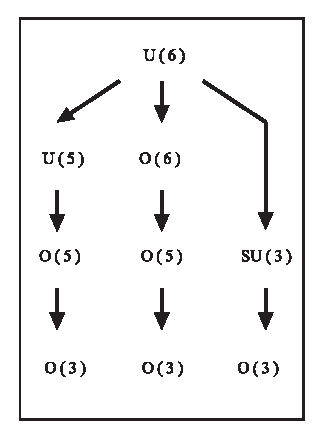
\includegraphics[scale=.65]{figure}
%
% If not, use
%\picplace{5cm}{2cm} % Give the correct figure height and width in cm
%
\caption{If the width of the figure is less than 7.8 cm use the \texttt{sidecapion} command to flush the caption on the left side of the page. If the figure is positioned at the top of the page, align the sidecaption with the top of the figure -- to achieve this you simply need to use the optional argument \texttt{[t]} with the \texttt{sidecaption} command}
\label{fig:1}       % Give a unique label
\end{figure}


\paragraph{Paragraph Heading} %
Instead of simply listing headings of different levels we recommend to let every heading be followed by at least a short passage of text. Furtheron please use the \LaTeX\ automatism for all your cross-references and citations as has already been described in Sect.~\ref{sec:2}.

Please note that the first line of text that follows a heading is not indented, whereas the first lines of all subsequent paragraphs are.

For typesetting numbered lists we recommend to use the \verb|enumerate| environment -- it will automatically render Springer's preferred layout.

\begin{enumerate}
\item{Livelihood and survival mobility are oftentimes coutcomes of uneven socioeconomic development.}
\begin{enumerate}
\item{Livelihood and survival mobility are oftentimes coutcomes of uneven socioeconomic development.}
\item{Livelihood and survival mobility are oftentimes coutcomes of uneven socioeconomic development.}
\end{enumerate}
\item{Livelihood and survival mobility are oftentimes coutcomes of uneven socioeconomic development.}
\end{enumerate}


\subparagraph{Subparagraph Heading} In order to avoid simply listing headings of different levels we recommend to let every heading be followed by at least a short passage of text. Use the \LaTeX\ automatism for all your cross-references and citations as has already been described in Sect.~\ref{sec:2}, see also Fig.~\ref{fig:2}.

Please note that the first line of text that follows a heading is not indented, whereas the first lines of all subsequent paragraphs are.

For unnumbered list we recommend to use the \verb|itemize| environment -- it will automatically render Springer's preferred layout.

\begin{itemize}
\item{Livelihood and survival mobility are oftentimes coutcomes of uneven socioeconomic development, cf. Table~\ref{tab:1}.}
\begin{itemize}
\item{Livelihood and survival mobility are oftentimes coutcomes of uneven socioeconomic development.}
\item{Livelihood and survival mobility are oftentimes coutcomes of uneven socioeconomic development.}
\end{itemize}
\item{Livelihood and survival mobility are oftentimes coutcomes of uneven socioeconomic development.}
\end{itemize}

\begin{figure}[t]
\sidecaption[t]
% Use the relevant command for your figure-insertion program
% to insert the figure file.
% For example, with the option graphics use
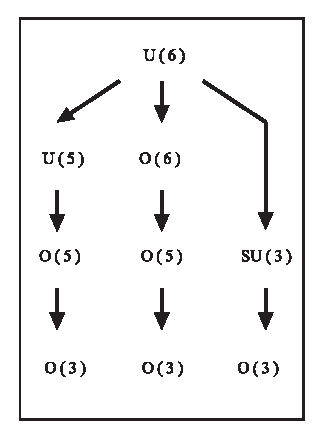
\includegraphics[scale=.65]{figure}
%
% If not, use
%\picplace{5cm}{2cm} % Give the correct figure height and width in cm
%
\caption{Please write your figure caption here}
\label{fig:2}       % Give a unique label
\end{figure}

\runinhead{Run-in Heading Boldface Version} Use the \LaTeX\ automatism for all your cross-references and citations as has already been described in Sect.~\ref{sec:2}.

\subruninhead{Run-in Heading Boldface and Italic Version} Use the \LaTeX\ automatism for all your cross-refer\-ences and citations as has already been described in Sect.~\ref{sec:2}\index{paragraph}.

\subsubruninhead{Run-in Heading Displayed Version} Use the \LaTeX\ automatism for all your cross-refer\-ences and citations as has already been described in Sect.~\ref{sec:2}\index{paragraph}.
% Use the \index{} command to code your index words
%
% For tables use
%
\begin{table}[!t]
\caption{Please write your table caption here}
\label{tab:1}       % Give a unique label
%
% For LaTeX tables use
%
\begin{tabular}{p{2cm}p{2.4cm}p{2cm}p{4.9cm}}
\hline\noalign{\smallskip}
Classes & Subclass & Length & Action Mechanism  \\
\noalign{\smallskip}\svhline\noalign{\smallskip}
Translation & mRNA$^a$  & 22 (19--25) & Translation repression, mRNA cleavage\\
Translation & mRNA cleavage & 21 & mRNA cleavage\\
Translation & mRNA  & 21--22 & mRNA cleavage\\
Translation & mRNA  & 24--26 & Histone and DNA Modification\\
\noalign{\smallskip}\hline\noalign{\smallskip}
\end{tabular}
$^a$ Table foot note (with superscript)
\end{table}
%
\section{Section Heading}
\label{sec:3}
% Always give a unique label
% and use \ref{<label>} for cross-references
% and \cite{<label>} for bibliographic references
% use \sectionmark{}
% to alter or adjust the section heading in the running head
Instead of simply listing headings of different levels we recommend to let every heading be followed by at least a short passage of text. Furtheron please use the \LaTeX\ automatism for all your cross-references and citations as has already been described in Sect.~\ref{sec:2}.

Please note that the first line of text that follows a heading is not indented, whereas the first lines of all subsequent paragraphs are.

If you want to list definitions or the like we recommend to use the Springer-enhanced \verb|description| environment -- it will automatically render Springer's preferred layout.

\begin{description}[Type 1]
\item[Type 1]{That addresses central themes pertainng to migration, health, and disease. In Sect.~\ref{sec:1}, Wilson discusses the role of human migration in infectious disease distributions and patterns.}
\item[Type 2]{That addresses central themes pertainng to migration, health, and disease. In Sect.~\ref{subsec:2}, Wilson discusses the role of human migration in infectious disease distributions and patterns.}
\end{description}

\subsection{Subsection Heading} %
In order to avoid simply listing headings of different levels we recommend to let every heading be followed by at least a short passage of text. Use the \LaTeX\ automatism for all your cross-references and citations citations as has already been described in Sect.~\ref{sec:2}.

Please note that the first line of text that follows a heading is not indented, whereas the first lines of all subsequent paragraphs are.

\begin{svgraybox}
If you want to emphasize complete paragraphs of texts we recommend to use the newly defined Springer class option \verb|graybox| and the newly defined environment \verb|svgraybox|. This will produce a 15 percent screened box 'behind' your text.

If you want to emphasize complete paragraphs of texts we recommend to use the newly defined Springer class option and environment \verb|svgraybox|. This will produce a 15 percent screened box 'behind' your text.
\end{svgraybox}


\subsubsection{Subsubsection Heading}
Instead of simply listing headings of different levels we recommend to let every heading be followed by at least a short passage of text. Furtheron please use the \LaTeX\ automatism for all your cross-references and citations as has already been described in Sect.~\ref{sec:2}.

Please note that the first line of text that follows a heading is not indented, whereas the first lines of all subsequent paragraphs are.

\begin{theorem}
Theorem text goes here.
\end{theorem}
%
% or
%
\begin{definition}
Definition text goes here.
\end{definition}

\begin{proof}
%\smartqed
Proof text goes here.
%\qed
\end{proof}

\paragraph{Paragraph Heading} %
Instead of simply listing headings of different levels we recommend to let every heading be followed by at least a short passage of text. Furtheron please use the \LaTeX\ automatism for all your cross-references and citations as has already been described in Sect.~\ref{sec:2}.

Note that the first line of text that follows a heading is not indented, whereas the first lines of all subsequent paragraphs are.
%
% For built-in environments use
%
\begin{theorem}
Theorem text goes here.
\end{theorem}
%
\begin{definition}
Definition text goes here.
\end{definition}
%
\begin{proof}
%\smartqed
Proof text goes here.
%\qed
\end{proof}
%
%
\begin{trailer}{Trailer Head}
If you want to emphasize complete paragraphs of texts in a \verb|Trailer Head| we recommend to
use  \begin{verbatim}\begin{trailer}{Trailer Head}
...
\end{trailer}\end{verbatim}
\end{trailer}
%
\begin{questype}{Questions}
If you want to emphasize complete paragraphs of texts in an \verb|Questions| we recommend to
use  \begin{verbatim}\begin{questype}{Questions}
...
\end{questype}\end{verbatim}
\end{questype}
%
%
\begin{important}{Important}
If you want to emphasize complete paragraphs of texts in an \verb|Important| we recommend to
use  \begin{verbatim}\begin{important}{Important}
...
\end{important}\end{verbatim}
\end{important}
%
\clearpage
\begin{warning}{Attention}
If you want to emphasize complete paragraphs of texts in an \verb|Attention| we recommend to
use  \begin{verbatim}\begin{warning}{Attention}
...
\end{warning}\end{verbatim}
\end{warning}

\begin{programcode}{Program Code}
If you want to emphasize complete paragraphs of texts in a \verb|Program Code| we recommend to
use

\verb|\begin{programcode}{Program Code}|

\verb|\begin{verbatim}...\end{verbatim}|

\verb|\end{programcode}|

\end{programcode}
%
\begin{tips}{Tips}
If you want to emphasize complete paragraphs of texts in a \verb|Tips| we recommend to
use  \begin{verbatim}\begin{tips}{Tips}
...
\end{tips}\end{verbatim}
\end{tips}
%
%
\begin{overview}{Overview}
If you want to emphasize complete paragraphs of texts in an \verb|Overview| we recommend to
use  \begin{verbatim}\begin{overview}{Overview}
...
\end{overview}\end{verbatim}
\end{overview}
\clearpage
\begin{backgroundinformation}{Background Information}
If you want to emphasize complete paragraphs of texts in a \verb|Background|
\verb|Information| we recommend to
use

\verb|\begin{backgroundinformation}{Background Information}|

\verb|...|

\verb|\end{backgroundinformation}|
\end{backgroundinformation}
\begin{legaltext}{Legal Text}
If you want to emphasize complete paragraphs of texts in a \verb|Legal Text| we recommend to
use  \begin{verbatim}\begin{legaltext}{Legal Text}
...
\end{legaltext}\end{verbatim}
\end{legaltext}
%
\begin{acknowledgement}
If you want to include acknowledgments of assistance and the like at the end of an individual chapter please use the \verb|acknowledgement| environment -- it will automatically render Springer's preferred layout.
\end{acknowledgement}
%
\section*{Appendix}
\addcontentsline{toc}{section}{Appendix}
%
When placed at the end of a chapter or contribution (as opposed to at the end of the book), the numbering of tables, figures, and equations in the appendix section continues on from that in the main text. Hence please \textit{do not} use the \verb|appendix| command when writing an appendix at the end of your chapter or contribution. If there is only one the appendix is designated ``Appendix'', or ``Appendix 1'', or ``Appendix 2'', etc. if there is more than one.

\begin{equation}
a \times b = c
\end{equation}
% Problems or Exercises should be sorted chapterwise
\section*{Problems}
\addcontentsline{toc}{section}{Problems}
%
% Use the following environment.
% Don't forget to label each problem;
% the label is needed for the solutions' environment
\begin{prob}
\label{prob1}
A given problem or Excercise is described here. The
problem is described here. The problem is described here.
\end{prob}

\begin{prob}
\label{prob2}
\textbf{Problem Heading}\\
(a) The first part of the problem is described here.\\
(b) The second part of the problem is described here.
\end{prob}

%%%%%%%%%%%%%%%%%%%%%%%% referenc.tex %%%%%%%%%%%%%%%%%%%%%%%%%%%%%%
% sample references
% %
% Use this file as a template for your own input.
%
%%%%%%%%%%%%%%%%%%%%%%%% Springer-Verlag %%%%%%%%%%%%%%%%%%%%%%%%%%
%
% BibTeX users please use
% \bibliographystyle{}
% \bibliography{}
%
%\biblstarthook{
\section{Styling of References}
In view of the parallel print and (chapter-wise) online publication of your book at \url{www.springerlink.com} it has been decided that -- as a genreral rule --  references should be sorted chapter-wise and placed at the end of the individual chapters. However, upon agreement with your contact at Springer you may list your references in a single seperate chapter at the end of your book. Deactivate the class option \texttt{sectrefs} and the \texttt{thebibliography} environment will be put out as a chapter of its own.\\\indent
References may be \textit{cited} in the text either by number (preferred) or by author/year.\footnote{Make sure that all references from the list are cited in the text. Those not cited should be moved to a separate \textit{Further Reading} section or chapter.} If the citatiion in the text is numbered, the reference list should be arranged in ascending order. If the citation in the text is author/year, the reference list should be \textit{sorted} alphabetically and if there are several works by the same author, the following order should be used:
\begin{enumerate}
\item all works by the author alone, ordered chronologically by year of publication
\item all works by the author with a coauthor, ordered alphabetically by coauthor
\item all works by the author with several coauthors, ordered chronologically by year of publication.
\end{enumerate}
The \textit{styling} of references\footnote{Always use the standard abbreviation of a journal's name according to the ISSN \textit{List of Title Word Abbreviations}, see \url{http://www.issn.org/en/node/344}} depends on the subject of your book:
\begin{itemize}
\item The \textit{two} recommended styles for references in books on \textit{mathematical, physical, statistical and computer sciences} are depicted in ~\cite{science-contrib, science-online, science-mono, science-journal, science-DOI} and ~\cite{phys-online, phys-mono, phys-journal, phys-DOI, phys-contrib}.
\item Examples of the most commonly used reference style in books on \textit{Psychology, Social Sciences} are~\cite{psysoc-mono, psysoc-online,psysoc-journal, psysoc-contrib, psysoc-DOI}.
\item Examples for references in books on \textit{Humanities, Linguistics, Philosophy} are~\cite{humlinphil-journal, humlinphil-contrib, humlinphil-mono, humlinphil-online, humlinphil-DOI}.
\item Examples of the basic Springer style used in publications on a wide range of subjects such as \textit{Computer Science, Economics, Engineering, Geosciences, Life Sciences, Medicine, Biomedicine} are ~\cite{basic-contrib, basic-online, basic-journal, basic-DOI, basic-mono}. 
\end{itemize}
%}

\begin{thebibliography}{99.}%
% and use \bibitem to create references.
%
% Use the following syntax and markup for your references if 
% the subject of your book is from the field 
% "Mathematics, Physics, Statistics, Computer Science"
%
% Contribution 
\bibitem{science-contrib} Broy, M.: Software engineering --- from auxiliary to key technologies. In: Broy, M., Dener, E. (eds.) Software Pioneers, pp. 10-13. Springer, Heidelberg (2002)
%
% Online Document
\bibitem{science-online} Dod, J.: Effective substances. In: The Dictionary of Substances and Their Effects. Royal Society of Chemistry (1999) Available via DIALOG. \\
\url{http://www.rsc.org/dose/title of subordinate document. Cited 15 Jan 1999}
%
% Monograph
\bibitem{science-mono} Geddes, K.O., Czapor, S.R., Labahn, G.: Algorithms for Computer Algebra. Kluwer, Boston (1992) 
%
% Journal article
\bibitem{science-journal} Hamburger, C.: Quasimonotonicity, regularity and duality for nonlinear systems of partial differential equations. Ann. Mat. Pura. Appl. \textbf{169}, 321--354 (1995)
%
% Journal article by DOI
\bibitem{science-DOI} Slifka, M.K., Whitton, J.L.: Clinical implications of dysregulated cytokine production. J. Mol. Med. (2000) doi: 10.1007/s001090000086 
%
%\bigskip

% Use the following (APS) syntax and markup for your references if 
% the subject of your book is from the field 
% "Mathematics, Physics, Statistics, Computer Science"
%
% Online Document
\bibitem{phys-online} J. Dod, in \textit{The Dictionary of Substances and Their Effects}, Royal Society of Chemistry. (Available via DIALOG, 1999), 
\url{http://www.rsc.org/dose/title of subordinate document. Cited 15 Jan 1999}
%
% Monograph
\bibitem{phys-mono} H. Ibach, H. L\"uth, \textit{Solid-State Physics}, 2nd edn. (Springer, New York, 1996), pp. 45-56 
%
% Journal article
\bibitem{phys-journal} S. Preuss, A. Demchuk Jr., M. Stuke, Appl. Phys. A \textbf{61}
%
% Journal article by DOI
\bibitem{phys-DOI} M.K. Slifka, J.L. Whitton, J. Mol. Med., doi: 10.1007/s001090000086
%
% Contribution 
\bibitem{phys-contrib} S.E. Smith, in \textit{Neuromuscular Junction}, ed. by E. Zaimis. Handbook of Experimental Pharmacology, vol 42 (Springer, Heidelberg, 1976), p. 593
%
%\bigskip
%
% Use the following syntax and markup for your references if 
% the subject of your book is from the field 
% "Psychology, Social Sciences"
%
%
% Monograph
\bibitem{psysoc-mono} Calfee, R.~C., \& Valencia, R.~R. (1991). \textit{APA guide to preparing manuscripts for journal publication.} Washington, DC: American Psychological Association.
%
% Online Document
\bibitem{psysoc-online} Dod, J. (1999). Effective substances. In: The dictionary of substances and their effects. Royal Society of Chemistry. Available via DIALOG. \\
\url{http://www.rsc.org/dose/Effective substances.} Cited 15 Jan 1999.
%
% Journal article
\bibitem{psysoc-journal} Harris, M., Karper, E., Stacks, G., Hoffman, D., DeNiro, R., Cruz, P., et al. (2001). Writing labs and the Hollywood connection. \textit{J Film} Writing, 44(3), 213--245.
%
% Contribution 
\bibitem{psysoc-contrib} O'Neil, J.~M., \& Egan, J. (1992). Men's and women's gender role journeys: Metaphor for healing, transition, and transformation. In B.~R. Wainrig (Ed.), \textit{Gender issues across the life cycle} (pp. 107--123). New York: Springer.
%
% Journal article by DOI
\bibitem{psysoc-DOI}Kreger, M., Brindis, C.D., Manuel, D.M., Sassoubre, L. (2007). Lessons learned in systems change initiatives: benchmarks and indicators. \textit{American Journal of Community Psychology}, doi: 10.1007/s10464-007-9108-14.
%
%
% Use the following syntax and markup for your references if 
% the subject of your book is from the field 
% "Humanities, Linguistics, Philosophy"
%
%\bigskip
%
% Journal article
\bibitem{humlinphil-journal} Alber John, Daniel C. O'Connell, and Sabine Kowal. 2002. Personal perspective in TV interviews. \textit{Pragmatics} 12:257--271
%
% Contribution 
\bibitem{humlinphil-contrib} Cameron, Deborah. 1997. Theoretical debates in feminist linguistics: Questions of sex and gender. In \textit{Gender and discourse}, ed. Ruth Wodak, 99--119. London: Sage Publications.
%
% Monograph
\bibitem{humlinphil-mono} Cameron, Deborah. 1985. \textit{Feminism and linguistic theory.} New York: St. Martin's Press.
%
% Online Document
\bibitem{humlinphil-online} Dod, Jake. 1999. Effective substances. In: The dictionary of substances and their effects. Royal Society of Chemistry. Available via DIALOG. \\
http://www.rsc.org/dose/title of subordinate document. Cited 15 Jan 1999
%
% Journal article by DOI
\bibitem{humlinphil-DOI} Suleiman, Camelia, Daniel C. O'Connell, and Sabine Kowal. 2002. `If you and I, if we, in this later day, lose that sacred fire...': Perspective in political interviews. \textit{Journal of Psycholinguistic Research}. doi: 10.1023/A:1015592129296.
%
%
%
%\bigskip
%
%
% Use the following syntax and markup for your references if 
% the subject of your book is from the field 
% "Computer Science, Economics, Engineering, Geosciences, Life Sciences"
%
%
% Contribution 
\bibitem{basic-contrib} Brown B, Aaron M (2001) The politics of nature. In: Smith J (ed) The rise of modern genomics, 3rd edn. Wiley, New York 
%
% Online Document
\bibitem{basic-online} Dod J (1999) Effective Substances. In: The dictionary of substances and their effects. Royal Society of Chemistry. Available via DIALOG. \\
\url{http://www.rsc.org/dose/title of subordinate document. Cited 15 Jan 1999}
%
% Journal article by DOI
\bibitem{basic-DOI} Slifka MK, Whitton JL (2000) Clinical implications of dysregulated cytokine production. J Mol Med, doi: 10.1007/s001090000086
%
% Journal article
\bibitem{basic-journal} Smith J, Jones M Jr, Houghton L et al (1999) Future of health insurance. N Engl J Med 965:325--329
%
% Monograph
\bibitem{basic-mono} South J, Blass B (2001) The future of modern genomics. Blackwell, London 
%
\end{thebibliography}


\activity{chapters/ch1Preliminary/ch1Preliminary}

\end{document}

%\chapter{Limits and Derivatives}

\documentclass{ximera}

\input{../../xmPreamble}
\author{Leon Kaganovskiy}
\title{Limits and Derivatives}
\begin{document}
\begin{abstract}
This chapter introduces two fundamental concepts of calculus: limits and derivatives. We use SageMath to explore these concepts numerically, symbolically, and graphically, helping us understand how a function behaves near a point and how its rate of change is defined. These ideas provide the foundation for differential calculus and for many of its applications in mathematics, science, and other fields.
\end{abstract}
\maketitle

%  \begin{image}[15cm] %\sidecaption[t]   remove ch2 etc reference local directory

\section{Limits and Continuity}

Let's begin limits consideration with a few examples of limits of function from numerical, analytical, and graphical perspectives.
In the function $f(x)=\frac{x^3-8}{x-2}$ below, the direct substitution produces an indeterminate expression $\frac{0}{0}$ at $x=2$,   Computing the function values close to the point of interest (using for loop) as well as graphing it convinces us that the limit exists and is equal to $12$.  Analytically, the numerator of $f(x)$ can be factored, which results in cancellation:
$$ f(x)=\frac{x^3-8}{x-2} = \frac{(x-2)(x^2+2x+4)}{x-2} =x^2+2x+4$$
SageMath can accomplish this with \texttt{factor()} and \texttt{full\_simplify()} commands.

\begin{programcode}{SageMath Code and Output:}
\begin{verbatim}
f(x)=(x^3-8)/(x-2);  show('f(x) = ',f(x))
L = [1.9,1.95,1.99,1.999,1.9999,2.0001,2.001,2.01,2.1]; 
n = len(L)
for i in range(n):
    show('For x = ', L[i], '  f(x) = ', f(L[i]))
L = limit(f(x),x=2); show('limit(f(x),x=2) = ', L)    

f(x)=(x^3-8)/(x-2);  show('f(x) = ',f(x))
g(x) = f(x).full_simplify()
show('f(x).full_simplify() = g(x) = ',g(x))
show('g(2) = ', g(2))  
plot(f(x),(x,-2,4), gridlines=True)
\end{verbatim}
\end{programcode}
The output is shown in Fig.~\ref{LimitCancel}
\begin{image}[15cm]
%\sidecaption[t]
\includegraphics[scale=.65]{LimitCancel.png}
\caption{Limits cancelling term}
\label{LimitCancel}       % Give a unique label
\end{image}


The steps done in the previous SageMath cell are algorithmic and well coded into a function def function\_values\(\) below.  Let's apply it to function $f(x)=\frac{\sqrt{x+4}-2}{x}$.  In this case, the numerator cannot be factored, but multiplying top and bottom by sign reciprocal works.   Note that in the code, the numerator must be expanded to cancel out 4 and then x.
$$f(x)=\frac{\sqrt{x+4}-2}{x} = \frac{(\sqrt{x+4}-2)(\sqrt{x+4}+2)}{x(\sqrt{x+4}+2)}=\frac{x+4-4}{x(\sqrt{x+4}+2)}=$$
$$\frac{x}{x(\sqrt{x+4}+2)}=\frac{1}{\sqrt{x+4}+2} \rightarrow \frac{1}{4} \ \ \ as \ x \rightarrow 0$$


\begin{programcode}{SageMath Code and Output:}
\begin{verbatim}
def function_values(x,f,x0):
    list = [x0-0.1,x0-0.01,x0-0.001,x0-0.0001,x0-0.00001,
            x0+0.00001,x0+0.0001,x0+0.001,x0+0.01,x0+0.1]
    n = len(list)
    show('f(x) = ',f)
    for i in range(n):
         show('For x = ', list[i], '  f(x) = ', f.subs(x=list[i]))
    L = limit(f,x=0); show('limit(f(x),x=0) = ', L) 
    
f = (sqrt(x+4)-2)/x
function_values(x,f,0)   
plot(f,(x,-4,4), figsize = (4,3), gridlines=True)

f(x)=(sqrt(x+4)-2)/x;  show('f(x) = ',f(x))
g(x)=expand((sqrt(x+4)-2)*(sqrt(x+4)+2))/(x*(sqrt(x+4)+2));  
show('g(x) = ',g(x).full_simplify())
show('g(0) = ', g(0))  
plot(f(x),(x,-2,4), gridlines=True)
\end{verbatim}
\end{programcode}
The output is shown in Fig.~\ref{LimitSquare}
\begin{image}[15cm]
%\sidecaption[t]
\includegraphics[scale=.65]{LimitSquare.png}
\caption{Limit Square}
\label{LimitSquare}       % Give a unique label
\end{image}


Next,  we illustrate three examples where the limits do not exist at $x=0$ whether due to jump, function going to infinity, or extreme oscillation, respectively.

\begin{programcode}{SageMath Code and Output:}
\begin{verbatim}
p1 = plot(abs(x)/x,(x,-2,2), ymin=-2, ymax=2, figsize =(5,4),
  legend_label= "abs(x)/x",color='red', gridlines=True)
p2 = plot(1/x,(x,-2,2), ymin=-10, ymax=10, figsize =(5,4),
  legend_label= "1/x",color='green', gridlines=True)
p3 = plot(sin(1/x),(x,-2,2), ymin=-1, ymax=1, figsize =(5,4),
  legend_label= "sin(1/x)",color='blue', gridlines=True)
G = graphics_array([[p1, p2, p3]])
G.show(figsize=[8, 3])
\end{verbatim}
\end{programcode}
The output is shown in Fig \ref{NoLimits}
\begin{image}[15cm]
%\sidecaption[t]
\includegraphics[scale=.65]{NoLimits.png}
\caption{Limit fails to exist due to jump, infinity, or extreme oscillation}
\label{NoLimits}       % Give a unique label
\end{image}


SageMath can compute special trigonometric limits.

\begin{programcode}{SageMath Code and Output:}
\begin{verbatim}
p1 = plot(sin(x)/x,(x,-4,4), ymin=-2, ymax=2, figsize =(5,4),
  legend_label= "sin(x)/x",color='red', gridlines=True)
p2 = plot((cos(x)-1)/x,(x,-2,2), ymin=-1, ymax=1, figsize =(5,4),
  legend_label= "(cos(x)-1)/x;",color='green', gridlines=True)
p3 = plot(sin(4*x)/x,(x,-2,2), ymin=-1, ymax=4, figsize =(5,4),
  legend_label= "sin(4*x)/x",color='blue', gridlines=True)
G = graphics_array([[p1, p2, p3]])
G.show(figsize=[8, 3])
L = limit(sin(x)/x,x=0); show('limit(sin(x)/x,x=0) = ', L)
L = limit((cos(x)-1)/x,x=0); show('limit((cos(x)-1)/x,x=0) = ', L)
L = limit(sin(4*x)/x,x=0); show('limit(sin(4*x)/x,x=0) = ', L)
\end{verbatim}
\end{programcode}
The output is shown in Fig \ref{TrigLimits}
\begin{image}[15cm]
%\sidecaption[t]
\includegraphics[scale=.65]{TrigLimits.png}
\caption{Trigonometric Limits}
\label{TrigLimits}       % Give a unique label
\end{image}


In previous chapter we illustrated the \texttt{piecewise()} function usage, however SageMath has trouble computing one sided limits for such a function.   Therefore, a better way to deal with a piecewise function for limits is to define two functions left and right of the breakpoint separately and plot them on respective domains.   The function below has a jump with different one-sided limits and, as a result, no limit at $x=1$.
\begin{programcode}{SageMath Code and Output:}
\begin{verbatim}
fL(x) = x-3;  fR(x)=x^2;   c = 1
show('fL(x)= ',fL(x),' fR(x) = ',fR(x),
     ' connecting at point c = ',c)
L = limit(fL(x),x=c,dir='-'); show('Left limit = ',L)
R = limit(fR(x),x=c,dir='+'); show('Right limit = ',R)
p1 = plot(fL(x),(x,-4,c), ymin=-10, ymax=10, 
          figsize = (4,3), gridlines=True)
p2 = plot(fR(x),(x, c,4), ymin=-10, ymax=10, gridlines=True)
(p1+p2).show()
\end{verbatim}
\end{programcode}
The output is shown in Fig \ref{LeftRightLimit}
\begin{image}[15cm]
%\sidecaption[t]
\includegraphics[scale=.65]{LeftRightLimit.png}
\caption{Piecewise function with a jump}
\label{LeftRightLimit}       % Give a unique label
\end{image}




%The idea of limit can be used to define absolute zero temperature.  The volume of a gas increases linearly with increasing temperature.   We use the known function to generate points and fit them back specifying a linear model and using \texttt{find\_fit()}.  In reality, the data are obtained experimentally.  Taking a limit of the resulting line approximation to zero volume, we obtain $T \approx -273^o$.   SageMath's ability to superimpose the plots is particularly useful here as we superimpose the scatterplot of data points and a regular linear function plot.
%
%\begin{programcode}{SageMath Code and Output:}
%\begin{verbatim}
%var('T,V,a,b')
%# artificially generated data points:
%V = 0.08213*T +  22.4324   
%Tv = [-100,-75,-50,-25,0,25,50,75,100]; 
%n = len(Tv); data = []  # initially data is an empty list
%for j in range(n) :
%    data.append( [Tv[j],N(V(T=Tv[j])) ] ) # data is appended 
%    
%model(T) = a*T + b
%sol = find_fit(data,model)   
%show(sol)
%a = sol[0].rhs();  b = sol[1].rhs(); 
%show('Temperature as function of volume: T= (V-',
%                            b,')/',round(a,3))
%show('Zero volume is achieved in the limit V->0 \n')
%show('at absolute zero temperature T = ',-b/a)
%
%p1 = scatter_plot( data, facecolor='red', gridlines=True) 
%p2 = plot(a*T + b,(T,-300,100),legend_label='fitted model',\
%         figsize = (5,4),color='green', gridlines=True) 
%
%plot_all = p1 + p2;  plot_all.show()
%\end{verbatim}
%\end{programcode}
%The output is shown in Fig \ref{AbsZero}
%\begin{image}[15cm]
%%\sidecaption[t]
%\includegraphics[scale=.65]{AbsZero.png}
%\caption{Using limits to find absolute zero temperature}
%\label{AbsZero}       % Give a unique label
%\end{image}

We can use SageMath to illustrate the Intermediate Value Theorem. The polynomial is negative at 0 and positive at 1, therefore it must have a root in between. The numerical routine \texttt{find\_root} finds this root with high accuracy.

\begin{programcode}{SageMath Code and Output:}
\begin{verbatim}
P(x)= 2*x^3+x-1;   show(P(x))
sol = find_root(P(x),0,1); 
show('the root is: ',sol)
plot(P(x),(x,-3,3), ymin=-10, ymax=10, 
     figsize = (4,3), gridlines=True)
\end{verbatim}
\end{programcode}
The output is shown in Fig \ref{IntermedValTheor}
\begin{image}[15cm]
%\sidecaption[t]
\includegraphics[scale=.65]{IntermedValTheor.png}
\caption{Intermediate value theorem}
\label{IntermedValTheor}       % Give a unique label
\end{image}


A rational function provides an excellent illustration of infinite one-sided limits at the location of vertical asymptotes as well as limits at infinity at the horizontal asymptotes.  In addition, it is very important to factor the numerator and denominator to look for possible cancellation implying that not all zeros the of original denominator lead to vertical asymptotes.   In the example below $x+2$ cancels out and there is no vertical asymptote at $x=-2$.  The highest power in the numerator and denominator are the same, so there is a horizontal asymptote at the ratio of coefficients $y=\frac{3}{2}$.
\begin{programcode}{SageMath Code and Output:}
\begin{verbatim}
N(x)=3*(x^2-4);   D(x)=2*(x^2-3*x-10); 
show('factored numerator = ', factor(N(x)))
show('factored denominator = ', factor(D(x)))
P(x)=N(x)/D(x); P(x)=P(x).full_simplify()
show('simplified rational function = ',P(x))
show('Zeros of denominator (up to cancellation)')
show(' give vertical asymptotes: ',solve(D(x)==0,x))
show(' limit(P(x),x=5, dir=-) = ', limit(P(x),x=5, dir='-'))
show(' limit(P(x),x=5, dir=+) = ', limit(P(x),x=5, dir='+'))
show('Possible Horizontal Asymptotes, left and and right limits at infinity:')
show(' limit(P(x),x=-oo) = ', limit(P(x),x=-oo))
show(' limit(P(x),x= oo) = ', limit(P(x),x= oo))     
plot([P(x),3/2],(x,-7,15), ymin=-20, ymax=20, \
 figsize=(4,3),color = ['blue','green'],gridlines=True)
\end{verbatim}
\end{programcode}
The output is shown in Fig \ref{RationalInfLimits}
\begin{image}[15cm]
%\sidecaption[t]
\includegraphics[scale=.65]{RationalInfLimits.png}
\caption{Rational function, infinite limits}
\label{RationalInfLimits}       % Give a unique label
\end{image}


The rational function below has the highest power of the numerator (linear=1) that is lower than the denominator's highest power 2 (quadratic), so $y=0$ is the horizontal asymptote.

\begin{programcode}{SageMath Code and Output:}
\begin{verbatim}
N(x)=3*(x^2-4);   D(x)=2*(x^2-3*x-10); 
N(x)=x;   D(x)=x^2-1; ZerosD = solve(D(x)==0,x); 
show('factored numerator = ', factor(N(x)))
show('factored denominator = ', factor(D(x)))
P(x)=N(x)/D(x); P(x)=P(x).full_simplify()
show('simplified rational function = ',P(x))
show('Zeros of denominator (up to cancellation)')
show(' give vertical asymptotes: ',solve(D(x)==0,x))
show('Possible Horizontal Asymptotes, left and')
show(' right limits at infinity:')
L = limit(P(x),x=-oo); R = limit(P(x),x=oo)
show(' limit(P(x),x=-oo) = ', L)
show(' limit(P(x),x= oo) = ', R)  
plot([P(x),L,R],(x,-7,7), ymin=-20, ymax=20, \
 figsize=(4,3),color = ['blue','green'],gridlines=True)
\end{verbatim}
\end{programcode}
The output is shown in Fig \ref{RationalLower}
\begin{image}[15cm]
%\sidecaption[t]
\includegraphics[scale=.65]{RationalLower.png}
\caption{Rational function, lower power on top}
\label{RationalLower}       % Give a unique label
\end{image}



%%%%%%%%%%%%%%%%%%%%%%%%%%%%%%%%%%%%%%%%%%%%%%%%%%%%%%%%%%%%%%%%%%%%%%%%%%%%%%%%%%%%%%%%%%%
\section{Differentiation}

%The SageMath code illustrates the steps in computing derivatives via limit definition.  Needless to say, SageMath can compute it directly, which will be shown shortly.
%
%\begin{programcode}{SageMath Code and Output:}
%\begin{verbatim}
%reset();  var('h')
%f(x)=x^3+2*x
%Numerator = f(x+h)-f(x);
%show('Numerator = ', Numerator)
%show(' factored: ',factor(Numerator))
%Quotient = Numerator/h; 
%show('Quotient = ', Quotient.full_simplify())
%fp(x) = limit(Quotient,h=0); 
%show('Limit of quotient = fp(x) = ',fp(x))
%\end{verbatim}
%\end{programcode}
%The output is shown in Fig \ref{DerivatLimit}
%\begin{image}[15cm]
%%\sidecaption[t]
%\includegraphics[scale=.65]{DerivatLimit.png}
%\caption{Computing derivative via limit definition}
%\label{DerivatLimit}       % Give a unique label
%\end{image}

SageMath has function \texttt{derivative()} which computes derivative automatically.  In the problem below we use it to obtain the equation of tangent line at a given point.  To illustrate the analytical solution:
$$  f(x)=x^3+2x \ \ \ \Rightarrow \ \ \ f'(x)=3x^2+2 $$
$$ at \ x_1=-1 \ \ \ \ \ y_1 = f(x_1)=f(-1)=(-1)^3+2(-1) = -3 $$
$$ slope=m=f'(x_1)=f'(-1)=3(-1)^2+2=5 \ \ \ \ \ \ \Rightarrow $$
$$ y_{tangent}=y_1+m(x-x_1)=-3+5(x+1)=5x+2   $$
The steps lend themselves well to an algorithm coded as a function below.

\begin{programcode}{SageMath Code and Output:}
\begin{verbatim}
def tang_line(x,f,x1,L,R,D,U):
    fp(x) = derivative(f(x),x)
    show('f(x) = ',f(x),'  its derivative  = ',fp(x))
    y1 = f(x1);  m = fp(x1);  b = y1-m*x1;
    show('y1 = ',y1,'  slope = m = ',m, ' y-intercept = b = ',b)
    ytang(x) = y1 + m*(x-x1);  
    show('tangent line = ',ytang(x))
    plot1 = plot(f(x) ,(x,L,R), ymin=D, ymax=U, figsize = (4,3),
       legend_label= "f(x)",color='red', gridlines=True)
    plot2 = plot(fp(x),(x,L,R), ymin=D, ymax=U, \
       legend_label= "fp(x)",color='blue', gridlines=True)
    plot3 = plot(ytang(x),(x,L,R), ymin=D, ymax=U,
       legend_label= "ytang(x)",color='green', gridlines=True)
    plot_all = plot1 + plot2 + plot3; plot_all.show()
    
f(x)=x^3+2*x;  x1 = -1
tang_line(x,f,x1,-3,3,-10,10)   
\end{verbatim}
\end{programcode}
The output is shown in Fig \ref{TangLineQubic}
\begin{image}[15cm]
%\sidecaption[t]
\includegraphics[scale=.65]{TangLineQubic.png}
\caption{Tangent line for cubic curve}
\label{TangLineQubic}       % Give a unique label
\end{image}

A similar tangent line problem with trigonometric functions is shown below.

\begin{programcode}{SageMath Code and Output:}
\begin{verbatim}
f(x)=3*sin(x)-2*cos(x);  x1 = pi/2
tang_line(x,f,x1,-2,6,-5,5)  
\end{verbatim}
\end{programcode}
The output is shown in Fig \ref{TangLineTrig}
\begin{image}[15cm]
%\sidecaption[t]
\includegraphics[scale=.65]{TangLineTrig.png}
\caption{Tangent line for a trigonometric function}
\label{TangLineTrig}       % Give a unique label
\end{image}


%In the Calculus course, special techniques for the derivatives of product and quotient are studied, but SageMath already has all these inside \texttt{derivative()} algorithms.  
%$$ f(x)=3x^2sin(x) \ \ \ \  \Rightarrow \ \ \ \ f'(x) = 6xsin(x) + 3x^2cos(x) $$
%$$ f \left( \frac{\pi}{2} \right)=3 \left( \frac{\pi}{2} \right)^2sin \left( \frac{\pi}{2} \right) = 3 \left( \frac{\pi}{2} \right)^2 $$
%$$ f' \left( \frac{\pi}{2} \right)=6\frac{\pi}{2} sin \left( \frac{\pi}{2} \right) + 3  \left( \frac{\pi}{2} \right)^2 cos \left( \frac{\pi}{2} \right)= 3\pi $$
%$$y_{tangent}=y_1+m(x-x_1)=3 \left( \frac{\pi}{2} \right)^2+3\pi \left(x- \frac{\pi}{2} \right) $$
%\begin{programcode}{SageMath Code and Output:}
%\begin{verbatim}
%f(x)=3*x^2*sin(x);  x1 = pi/2
%tang_line(x,f,x1,-1,3,-5,25)  
%\end{verbatim}
%\end{programcode}
%The output is shown in Fig \ref{DerivProdRule}
%\begin{image}[15cm]
%%\sidecaption[t]
%\includegraphics[scale=.65]{DerivProdRule.png}
%\caption{Tangent line and derivative illustrating product rule}
%\label{DerivProdRule}       % Give a unique label
%\end{image}
%
%For the rational function below, the quotient rule gives:
%$$ f(x)=\frac{3x^5-1}{x^2+1} \ \ \ \ \ \Rightarrow \ \ \ \ \  f'(x)=\frac{15x^4(x^2+1) -(3x^5-1)2x }{(x^2+1)^2}$$
%As often happens with Computer Algebra Systems (CAS), the SageMath output looks slightly different but mathematically equivalent.
%
%\begin{programcode}{SageMath Code and Output:}
%\begin{verbatim}
%f(x)=(3*x^5-1)/(x^2+1);  x1 = 1 
%tang_line(x,f,x1,-1,3,-5,25)   
%\end{verbatim}
%\end{programcode}
%The output is shown in Fig \ref{DerivQuotient}
%\begin{image}[15cm]
%%\sidecaption[t]
%\includegraphics[scale=.65]{DerivQuotient.png}
%\caption{Tangent line and derivative illustrating quotient rule}
%\label{DerivQuotient}       % Give a unique label
%\end{image}


The problem below considers a classic application of derivatives to Physics.  A ball is thrown up with a speed $48 \ ft/s$.   The gravity acceleration in these units is $32 \ ft/s^2$ and is directed down.  The standard formula $h(t)=v_0t+at^2/2$ for height is used and its derivative gives the ball's velocity.  The time when this velocity is zero gives the highest point in the ball's trajectory.  it is easy to find analytically, but in the SageMath code below we use \texttt{solve(v(t)==0,t)} to find this time and extract the solution with \texttt{sol[0].rhs()} rounding it to 3 digits with \texttt{N(..,3)}.  We plug it back into the height function with \texttt{h(tm)} to find the maximum height.
\begin{programcode}{SageMath Code and Output:}
\begin{verbatim}
reset(); var('t')
g = 32;  v0=48; 
h(t) = v0*t-g*t^2/2
v(t) = derivative(h(t),t)
sol = solve(v(t)==0,t);  tm = N(sol[0].rhs(),3)
show('Highest point: h(tm) = ',h(tm), ' at time tm = ',tm)
a = 0; b = 3.1; c = -60; d = 55; # bounds for the plot box
plot1 = plot(h(t),(t,a,b), ymin=c, ymax=d, figsize = (4,3),\
     legend_label= "h(t)",color='red' , gridlines=True)
plot2 = plot(v(t),(t,a,b), ymin=c, ymax=d, \
     legend_label= "v(t)",color='blue', gridlines=True)
plot_all = plot1 + plot2;  plot_all.show()
\end{verbatim}
\end{programcode}
The output is shown in Fig \ref{Projectile}
\begin{image}[15cm]
%\sidecaption[t]
\includegraphics[scale=.65]{Projectile.png}
\caption{Vertical projectile height and velocity }
\label{Projectile}       % Give a unique label
\end{image}


As a business application, in the SageMath cell below, we consider data on company sales after the introduction of a new popular product.   A quadratic model is fit to the sales and its rate of change (derivative) is computed and plotted.   It can be used to understand the sales better.   Note how  \texttt{data = list(zip(Tv, Sv))} was used to zip the two data columns together.
\begin{programcode}{SageMath Code and Output:}
\begin{verbatim}
var('t, a0, a1, a2')

# Data
Tv = range(11)
Sv = [3.2, 4.3, 5.8, 7.1, 10.1, 13.7, 16.4, 20.7, 28.1, 37.4, 50.2]
data = list(zip(Tv, Sv))

# Quadratic model and fitted coefficients
model(t) = a0 + a1*t + a2*t^2
sol = find_fit(data, model)

a0, a1, a2 = [round(sol[i].rhs(), 2) for i in range(3)]

# Fitted model and its derivative
Sfit(t) = a0 + a1*t + a2*t^2
Sfitp(t) = derivative(Sfit(t), t)

show('Coefficients: ', (a0, a1, a2))
show('Fitted model: ', Sfit(t))
show('Rate of sales: ', Sfitp(t))

p1 = scatter_plot(data, facecolor='red', gridlines=True)
p2 = plot(Sfit, (t, 0, 10), color='green', 
               legend_label='Fitted sales', gridlines=True)
(p1 + p2).show(figsize=5)

plot(Sfitp, (t, 0, 10), color='blue', title='Rate of sales',
     axes_labels=['t', "S'(t)"], gridlines=True).show(figsize=5)
\end{verbatim}
\end{programcode}
The output is shown in Fig \ref{SalesQuadFit}
\begin{image}[15cm]
%\sidecaption[t]
\includegraphics[scale=.65]{SalesQuadFit.png}
\caption{Sales quadratic fit }
\label{SalesQuadFit}       % Give a unique label
\end{image}

The next few examples illustrate the chain rule.
\begin{programcode}{SageMath Code and Output:}
\begin{verbatim}
f(x)=sqrt(7*x^3-3*x^2+5*x-4); fp(x) = derivative(f(x),x)
show('f(x) = ',f(x)); show(' its derivative  = ',fp(x))
f(x)=-5/(x^2-7*x+2)^4;  fp(x) = derivative(f(x),x)
show('f(x) = ',f(x)); show(' its derivative  = ',fp(x))
f(x)= x*sqrt(1-x^2);  fp(x) = derivative(f(x),x)
show('f(x) = ',f(x)); show(' its derivative  = ',fp(x))
f(x)= (3*x+1)/(1-x^2)^(1/3); fp(x) = derivative(f(x),x)
show('f(x) = ',f(x)); show(' its derivative  = ',fp(x))
f(x)= sin(3*x^5-6*x^2-4*x+2);  fp(x) = derivative(f(x),x)
show('f(x) = ',f(x)); show(' its derivative  = ',fp(x))
f(x)= (sin(3*x^2-6*x+2))^3;  fp(x) = derivative(f(x),x)
show('f(x) = ',f(x)); show(' its derivative  = ',fp(x))
\end{verbatim}
\end{programcode}
The output is shown in Fig \ref{ChainRule}
\begin{image}[15cm]
%\sidecaption[t]
\includegraphics[scale=.65]{ChainRule.png}
\caption{Chain rule examples}
\label{ChainRule}       % Give a unique label
\end{image}

In the problem below we illustrate implicit derivative.   The analytical method is to differentiate the equation in $x$ 
keeping in mind that $y$ depends on $x$ and solve for $y'$.   Let's first illustrate it analytically.
$$ y^3 - 2y^2x + 4yx^2 =3 \ \ \ \Rightarrow  \ \ \ \  3y^2y'-4yy'x-2y^2+4y'x^2+8yx=0 \ \ \ \Rightarrow $$
$$ y'(3y^2 -4yx+4x^2)  + (8yx-2y^2) =0  \ \ \ \Rightarrow  \ \ \ \ y' = - \frac{ 8xy-2y^2}{3y^2 -4xy+4x^2} $$
However, from the computational point of view, it is much easier to apply the formula with partial derivatives from 
Multivariate Calculus: $y'(x) = -\frac{F_x(x,y)}{F_y(x,y)}$.   In addition, we plot tangent line.

\begin{programcode}{SageMath Code and Output:}
\begin{verbatim}
F(x,y) = y^3 - 2*y^2*x + 4*y*x^2 - 3;  
x1 = 1;  y1 = 1;
Fx(x,y) = derivative(F(x,y),x);   
Fy(x,y) =derivative(F(x,y),y); 
show('F(x,y) = ', F(x,y))
show('  Fx(x,y) = ', Fx(x,y))
show('  Fy(x,y) = ', Fy(x,y)); 
yp(x,y) = - Fx(x,y)/Fy(x,y);   
show('yp(x,y) = - Fx(x,y)/Fy(x,y) = ', yp(x,y)); 
m = yp(x1,y1);  show('slope = m = ',m)
ytang(x) = y1 + m*(x-x1);  show('tangent line = ',ytang(x))
a = -5; b = 5; c = -5; d = 5; # bounds for the plot box
plot1 = implicit_plot(F(x,y),(x,a,b), (y,c,d), figsize = (5,4),\
    legend_label= "implicit plot",color='red', gridlines=True)
plot2 = plot(ytang(x),(x,a,b), ymin=c, ymax=d, \
    legend_label= "ytang(x)",color='green', gridlines=True)
plot_all = plot1 + plot2;  plot_all.show()
\end{verbatim}
\end{programcode}
The output is shown in Fig \ref{Implicit}
\begin{image}[15cm]
%\sidecaption[t]
\includegraphics[scale=.65]{Implicit.png}
\caption{Implicit differentiation}
\label{Implicit}       % Give a unique label
\end{image}


We illustrate related rates with a classic problem of a spherical balloon.   An air is pumped into a spherical balloon at 3 cubic 
meters per minute.  Find the rate of change of radius when the volume is 30 cubic meters.
$$ V=\frac{4}{3}\pi r^3  \ \ \ \ \Rightarrow \ \ \ \  \frac{dV}{dr} = 4\pi r^2 \ \ \ \ \Rightarrow \ \ \ \ 
 \frac{dV}{dt} =\frac{dV}{dr} \frac{dr}{dt} =4\pi r^2 \frac{dr}{dt} \ \ \ \Rightarrow $$
$$ \frac{dr}{dt} = \frac{1}{4\pi r^2}\frac{dV}{dr}   \ \ \ \  \  \text{also} \ \ \ \  r_1=\left( \frac{3V_1}{4\pi} \right)^{1/3}  
\ \ \ \ \Rightarrow \ \ \ \ \frac{dr}{dt}_{r=r_1} = \frac{1}{4\pi r_1^2}\frac{dV}{dt} $$
\begin{programcode}{SageMath Code and Output:}
\begin{verbatim}
var('V,r')
V(r) = 4/3*pi*r^3;    Vp(r) = derivative(V(r),r)
show('V(r) = ', V(r),'     Vp(r) = ', Vp(r) ); 
V1 = 30;  Vt1 = 3;  r1 = N((3*V1/(4*pi))^(1/3));
rt1 = N(Vt1/Vp(r1)); 
print('the rate of change of radius when volume is = ', V1)
print(' and radius is  r = {:.3f} is = rt1 = {:.3f}'.
      format(r1,rt1))
\end{verbatim}
\end{programcode}
The output is shown in Fig \ref{RelatedRatesSphere}
\begin{image}[15cm]
%\sidecaption[t]
\includegraphics[scale=.65]{RelatedRatesSphere.png}
\caption{Related rates spherical baloon}
\label{RelatedRatesSphere}       % Give a unique label
\end{image}



Here is another classical related rate problem.   An airplane is flying horizontally directly over a radar station at the height $h=10$ miles.   Let $s$ denote the direct distance from the plane to the station.    Assume $s$ is decreasing at 500 miles/hour.   What is the speed of the plane when the distance is 14 miles?    Let x be the horizontal distance to the station.   From the Pythagorean theorem and chain rule, we obtain:
$$ s^2 = x^2 + h^2 \ \ \ \ \  \Rightarrow \ \ \ \ \  x = \sqrt{s^2-h^2} \ \ \  also $$
$$ 2s\frac{ds}{dt}=2x\frac{dx}{dt}+0 \ \ \ \  \Rightarrow \ \ \ \ \  \frac{dx}{dt} = \frac{s}{x}\frac{ds}{dt}= \frac{s}{\sqrt{s^2-h^2}}\frac{ds}{dt} $$
\begin{programcode}{SageMath Code and Output:}
\begin{verbatim}
var('s')
h1 = 10; st = 500;  s1 = 14;  st1 = -500;
x1 = N(sqrt(s1^2-h1^2));  xt1 = N(s1/x1*st1)
print('At the distance s1= ', s1)
print('  horizontal distance x1 = ',x1)
print('  and velocity =  xt1 = ',xt1)
\end{verbatim}
\end{programcode}
The output is shown in Fig \ref{RelatedRatesPlane}
\begin{image}[15cm]
%\sidecaption[t]
\includegraphics[scale=.65]{RelatedRatesPlane.png}
\caption{Related rates airplane flying over a radar}
\label{RelatedRatesPlane}       % Give a unique label
\end{image}







%%%%%%%%%%%%%%%%%%%%%%%%%%%%%%%%%%%%%%%%%%%%%%%%%%%%%%%%%%%%%%%%%%%%%%%%%%%%%%%%%%%%%%%%%%%
\section{Applications of Differentiation}

One of the main applications of derivatives is graphing functions.   In the regions where the first derivative is positive, the function increases, while the negative derivative implies a decreasing function.  Analogously, the regions of positive/negative 2nd derivative imply concave up/down behavior.  SageMath code below automates the process of finding 1st and 2nd derivatives and their zeros.  It also plots them in different colors to see the sign changes and the resulting function graph.   Let's begin with a simple polynomial.
$$ f(x) = 3x^4-6x^3 \ \ \ \ \ \Rightarrow \ \ \ \ \ f'(x) = 12x^3-18x^2 = 6x^2(2x-3) \ \ \ \ \ \Rightarrow \ \ \ \ \ $$
$$ f''(x) =36x^2-36x=36x(x-1)  $$
The steps are algorithmic and well-coded into a function \texttt{graphing\_func(x,f,L,R,D,U)}.  Note that left, right, up, and down graph limits may have to be adjusted once critical points of the function ($f'(x)$ - zero or fails to exist) are determined.  

\begin{programcode}{SageMath Code and Output:}
\begin{verbatim}
def graphing_func(x,f,L,R,D,U):
    fp(x) = derivative(f(x),x); 
    fpp(x) = derivative(fp(x),x)
    show('f(x) = ', f(x))
    show('  derivative = fp(x) = ', fp(x))
    show('  factored form is =', factor(fp(x)) )
    show('  2nd derivative = fpp(x) = ', fpp(x))
    show('  factored form is =', factor(fpp(x)) )
    solp  = solve(fp(x)==0 ,x); 
    show('Zeros of derivative are: ', solp)
    solpp = solve(fpp(x)==0,x); 
    show('Zeros of 2nd derivative are: ', solpp)
    plot1 = plot(f(x)  ,(x,L,R), ymin=D, ymax=U, figsize = (5,4), \
        legend_label= "f(x)",color='red', gridlines=True)
    plot2 = plot(fp(x) ,(x,L,R), ymin=D, ymax=U, \
        legend_label= "fp(x)",color='blue', gridlines=True)
    plot3 = plot(fpp(x),(x,L,R), ymin=D, ymax=U, \
        legend_label= "fpp(x)",color='green', gridlines=True)
    plot_all = plot1 + plot2 + plot3; plot_all.show()
    
f(x) = 3*x^4-6*x^3; 
graphing_func(x,f,-3,3,-10,10)
\end{verbatim}
\end{programcode}
The output is shown in Fig \ref{GraphPolyn}
\begin{image}[15cm]
%\sidecaption[t]
\includegraphics[scale=.65]{GraphPolyn.png}
\caption{Graphing a polynomial function using derivatives}
\label{GraphPolyn}       % Give a unique label
\end{image}


The function below, in addition to min/max and inflection points, shows vertical and horizontal asymptotes.  Vertical asymptote is at the zero of denominator $x=-1$.   The highest power of the numerator (1) is lower than the highest power of the denominator (2), therefore x-axis ($y=0$) is the horizontal asymptote.
$$ f(x) = \frac{x}{(x+1)^2}$$
$$ f'(x) =  \frac{1(x+1)^2-x2(x+1)}{(x+1)^4}=  \frac{1(x+1)-2x}{(x+1)^3} =  \frac{1-x}{(x+1)^3} $$
$$ f''(x) = \frac{-1(x+1)^3-(1-x)3(x+1)^2}{(x+1)^3}= \frac{-1(x+1)-(1-x)3}{(x+1)^4} = $$
$$ \frac{2x-4}{(x+1)^4}= \frac{2(x-2)}{(x+1)^4}$$

\begin{programcode}{SageMath Code and Output:}
\begin{verbatim}
f(x) = x/(x+1)^2; 
graphing_func(x,f,-5,5,-3,3)
\end{verbatim}
\end{programcode}
The output is shown in Fig \ref{GraphAsympt}
\begin{image}[15cm]
%\sidecaption[t]
\includegraphics[scale=.65]{GraphAsympt.png}
\caption{Graphing a function with asymptotes}
\label{GraphAsympt}       % Give a unique label
\end{image}

In the problem below a case of infinite derivative is illustrated.  It results in a cusp point at $x=0$.    
$$ f(x) = x-x^{2/3} \ \ \ \ \ \Rightarrow \ \ \ \ \ $$
$$ f'(x) = 1-\frac{2}{3}x^{-1/3}= 1-\frac{2}{3x^{1/3}} = \frac{3x^{1/3}-2}{3x^{1/3}}=0 \ \ gives \ \left(\frac{2}{3} \right)^3=\frac{8}{27} $$
$$ f''(x) = \frac{2}{9}x^{-4/3}= \frac{2}{9x^{4/3}} \ \ \ \ \text{never 0, but} \ x= 0 \ \text{is critical point}$$
Unfortunately, at this point, Sage cannot properly handle plotting fractional powers for negative x's, so we only plotted it for a positive interval.

\begin{programcode}{SageMath Code and Output:}
\begin{verbatim}
f(x) = x-x^(2/3);   
graphing_func(x,f,0,5,-3,4)
\end{verbatim}
\end{programcode}
The output is shown in Fig \ref{GraphCusp}
\begin{image}[15cm]
%\sidecaption[t]
\includegraphics[scale=.65]{GraphCusp.png}
\caption{Graphing a function with cusp (infinite derivative)}
\label{GraphCusp}       % Give a unique label
\end{image}

An interesting property of the function $f(x) = \frac{x}{\sqrt{x^2+4}}$ below is that it has different left and right horizontal asymptotes:
$$ lim_{x \rightarrow -\infty} f(x) = lim_{x \rightarrow -\infty} \frac{x}{\sqrt{x^2+4}}  = $$
$$ lim_{x \rightarrow -\infty} \frac{x}{\sqrt{x^2(1+4/x^2)}} = lim_{x \rightarrow -\infty} \frac{x}{-x\sqrt{1+4/x^2}} =-1$$
$$ lim_{x \rightarrow \infty} f(x) = lim_{x \rightarrow \infty} \frac{x}{\sqrt{x^2+4}}  =$$
$$ lim_{x \rightarrow \infty} \frac{x}{\sqrt{x^2(1+4/x^2)}} = lim_{x \rightarrow \infty} \frac{x}{x\sqrt{1+4/x^2}} =1$$
The first derivative allows some important square root simplifications:
$$ f'(x) = \frac{\sqrt{x^2+4}-x\frac{2x}{2\sqrt{x^2+4}}}{(\sqrt{x^2+4})^2} =\frac{x^2+4-x^2}{(\sqrt{x^2+4})^3} = \frac{4}{(x^2+4)^{3/2}} >0 $$
The first derivative is always positive resulting in a strictly increasing function.
The 2nd derivative is easier to compute as a power function and a chain rule as opposed to quotient rule used for the 1st derivative:
$$f''(x) = 4\left(-\frac{3}{2}\right)(x^2+4)^{-5/2}2x = -\frac{12x}{(x^2+4)^{5/2}}$$
The resulting 2nd derivative changes sign at 0, which is the inflection point.

\begin{programcode}{SageMath Code and Output:}
\begin{verbatim}
f(x) = x/sqrt(x^2+4);   
graphing_func(x,f,-6,6,-1,1)
\end{verbatim}
\end{programcode}
The output is shown in Fig \ref{GraphSqrt}
\begin{image}[15cm]
%\sidecaption[t]
\includegraphics[scale=.65]{GraphSqrt.png}
\caption{Different horizontal asymptotes}
\label{GraphSqrt}       % Give a unique label
\end{image}


The code below illustrates mean value theorem.   The function $f(x)=3-\frac{5}{x}$ is differentiable on the interval $[1,7]$.  The slope of the secant line on this interval is $m=\frac{f(7)-f(1)}{7-1}=\frac{5}{7}$.   According to the Mean Value Theorem, there should be at least one $x=x_1$ such that $f'(x_1)=\frac{5}{7}$.   In the code below we find such $x_1$ and plot the corresponding secant line and the parallel tangent line.
\begin{programcode}{SageMath Code and Output:}
\begin{verbatim}
f(x) = 3-5/x;  
a = 1; b = 7;  c = -4; d = 4; # bounds for the plot box
fp(x) = derivative(f(x),x);  
show('f(x) = ', f(x))
show('  derivative = fp(x) = ', fp(x) )
secant_slope = (f(b)-f(a))/(b-a)
sol  = solve(fp(x)==secant_slope ,x);
show("f'(x)=secant_slope: ", sol)
x1 = sol[1].rhs();  
show('secant slope = ',secant_slope)
show('  is matched at x1 = ',x1)
y_sec(x) = f(a) + secant_slope*(x-a)
y_tang(x) = f(x1) + + secant_slope*(x-x1)
show('secant line equation: y = ',y_sec(x))
show('   tangent line equation: y = ',y_tang(x))
plot1 = plot(f(x) ,(x,a,b), ymin=c, ymax=d, figsize = (4,3),\
   legend_label= "f(x)",color='red', gridlines=True)
plot2 = plot(y_sec(x),(x,a,b), ymin=c, ymax=d, \
   legend_label= "y_sec(x)",color='blue', gridlines=True)
plot3 = plot(y_tang(x),(x,a,b), ymin=c, ymax=d, \
   legend_label= "y_tang(x)",color='green', gridlines=True)
plot_all = plot1 + plot2 + plot3; plot_all.show()
\end{verbatim}
\end{programcode}
The output is shown in Fig \ref{MeanValTheor}
\begin{image}[15cm]
%\sidecaption[t]
\includegraphics[scale=.65]{MeanValTheor.png}
\caption{Mean value theorem}
\label{MeanValTheor}       % Give a unique label
\end{image}


One of the main applications of derivatives is optimization problems.   For example, In the SageMathcode below we consider the following profit maximization application.  The daily demand function for x LED lights sold by a major retailer is $p(x)=880-0.75x$ dollars, and the average cost of sales is $\bar{C}(x)= \frac{C(x)}{x}=220+2x$ dollars. Find the quantity that will maximize profit, the selling price at that quantity, and the maximum profit.
$$ Cost = C(x) = \bar{C}(x)x=220x+2x^2 \ \ \ \ \ \ \  $$
$$ Revenue = R(x) = p(x)x=880x-0.75x^2 \ \ \ \Rightarrow \ \ \  $$
$$ Profit = P(x)=R(x)-C(x)= -2.75x^2+660x$$

\begin{programcode}{SageMath Code and Output:}
\begin{verbatim}
p(x) = 880-3/4*x;  Cbar(x) = 220+2*x;   C(x) = expand(Cbar(x)*x);  
show('Demand = p = ',p(x))
show(' Average Cost = Cbar = ',Cbar(x))
show(' Cost = C(x) =', C(x))
R(x) = expand(p(x)*x);  P(x) = expand(R(x)-C(x));
show(' Revenue = R(x) = ', R(x))
show(' Profit = P(x) = ', P(x))
Pd(x) = derivative(P(x),x);  
show('Profit derivative = Pd(x) = ', Pd(x))
sol = solve(Pd(x)==0,x); xm = sol[0].rhs();  
show("Solving P'(x) = 0, sol = ", sol)
show('Max profit P(xm) = ', P(xm))
show(' achieved at # of items xm = ', xm)
show(' sold at price p(xm) =',p(xm))

a = 0; b = 250; c = -1; d = 70000; # bounds for the plot box
plot1 = plot(R(x),(x,a,b), ymin=c, ymax=d, figsize = (5,4),\
  legend_label= "Revenue",color='red', gridlines=True)
plot2 = plot(C(x),(x,a,b), ymin=c, ymax=d, \
  legend_label= "Cost",color='blue', gridlines=True)
plot3 = plot(P(x),(x,a,b), ymin=c, ymax=d, \
  legend_label= "Profit",color='green', gridlines=True)
plot_all = plot1 + plot2 + plot3; plot_all.show()
\end{verbatim}
\end{programcode}
The output is shown in Fig \ref{MaxProfit}
\begin{image}[15cm]
%\sidecaption[t]
\includegraphics[scale=.65]{MaxProfit.png}
\caption{Max Profit}
\label{MaxProfit}       % Give a unique label
\end{image}


Another standard optimization problem is as follows.  A manufacturer wants to design an open top box having a square base $x$ and volume of 500 cubic feet.   The sides cost 2 dollars per square feet and the bottom 3 dollars per square feet.  What dimensions will produce a box with minimal cost?
$$ Volume = V=L\cdot W \cdot H= x \cdot x \cdot H=500 \ \ \Rightarrow H = \frac{500}{x^2} $$
$$ Cost =C(x)= 3\cdot x^2+ 2\cdot 4xH = 3x^2 + 8x \frac{500}{x^2}  = 3x^2+ \frac{4000}{x}=3x^2+4000x^{-1}$$
$$ C'(x) = 6x - 4000x^{-2} = \frac{6x^3-4000}{x^2}=0 \ \ \ \Rightarrow x_m = \left(\frac{4000}{6}\right)^{1/3}  $$

\begin{programcode}{SageMath Code and Output:}
\begin{verbatim}
V = 500; pb = 3;  ps = 2;   # problem parameters
H = V/x^2;   C(x) = expand(pb*x^2 + ps*4*x*H);   
Cp(x) = derivative(C(x),x);  
show('Cost function = C(x) = ', C(x))
show(' derivative = Cp(x) = ',Cp(x) )
xm = find_root(Cp(x)==0,0,500);  Hm = V/xm^2;
show('Min cost C(xm) = ', C(xm))
show('achieved at the square dimension = xm = ', xm)
show(' and height = H =',Hm)

a = 0; b = 20; c = -1000; d = 2000; # plot bounds
plot1 = plot(C(x),(x,a,b), ymin=c, ymax=d, figsize = (5,4), \
  legend_label= "C(x)",color='red', gridlines=True)
plot2 = plot(Cp(x),(x,a,b), ymin=c, ymax=d, \
  legend_label= "Cp(x)",color='blue', gridlines=True)
plot_all = plot1 + plot2; plot_all.show()
\end{verbatim}
\end{programcode}
The output is shown in Fig \ref{OptimizeBox}
\begin{image}[15cm]
%\sidecaption[t]
\includegraphics[scale=.65]{OptimizeBox.png}
\caption{Open box with minimal cost}
\label{OptimizeBox}       % Give a unique label
\end{image}


Yet another classic optimization problem is  of a guy who needs to get from a village on one side of a 4 km wide river to the other 10 km downstream.   He can row across the river at 7 km/h and quickly walk on the river bank at 10 km/h.   Where should he land to reach his target as soon as possible? 
If we let $x$ to be the distance downstream, the rowing time is $\frac{\sqrt{x^2+16}}{7}$ and the time on the other bank of the river is $\frac{10-x}{10}$.  Their sum must be minimized.   Note that the parameters are specified in the 1st line of the code, so that they can be easier changed as needed.   Generally, it is a bad idea to hardcode the numbers into the problem.
\begin{programcode}{SageMath Code and Output:}
\begin{verbatim}
d1 = 4; v1 = 7;  d2 = 10; v2 = 10;   # parameters
T(x) = expand(sqrt(x^2+d1^2)/v1 + (d2-x)/v2);   
Tp(x) = derivative(T(x),x);  
show('Time function to optimize = T(x) = ', T(x))
show(' derivative = Tp(x) = ',Tp(x) )
xm = find_root(Tp(x)==0,0,d2);  
show('min T(xm) = ', round(T(xm),4), \
     ' is achieved at xm = ',round(xm,4))

a = 0; b = 10; c = -1; d = 2; # plot bounds
plot1 = plot(T(x),(x,a,b), ymin=c, ymax=d, \
   legend_label= "T(x)",color='red', gridlines=True)
plot2 = plot(Tp(x),(x,a,b), ymin=c, ymax=d, \
   legend_label= "Tp(x)",color='blue', gridlines=True)
plot_all = plot1 + plot2; plot_all.show()
\end{verbatim}
\end{programcode}
The output is shown in Fig \ref{OptimizeRiver}
\begin{image}[15cm]
%\sidecaption[t]
\includegraphics[scale=.65]{OptimizeRiver.png}
\caption{Mimimize time of crossing a river and walking}
\label{OptimizeRiver}       % Give a unique label
\end{image}


One more application of derivatives involves using an equation of the tangent line developed before to provide a linear approximation in the neighborhood of a given point.  For example:
$$ f(x) = \sqrt{x+7} \ \ \ \Rightarrow f'(x) = \frac{1}{2\sqrt{x+7}}$$
$$ f(x_1=2)= \sqrt{2+7}=3 \ \ and \ \ f'(x_1) =f'(2) = \frac{1}{2\sqrt{2+7}}=  \frac{1}{6}  \ \Rightarrow$$
$$ y_{tang}(x) = f(x_1)+f'(x_1)(x-x1) = 3+\frac{1}{6}(x-2) = \frac{1}{6}x + \frac{8}{3}$$
The SageMath code below calculates this tangent line approximation and compares the exact function value to the linear approximation at a nearby point.   It can be seen from the graph that the approximation is inherently local and gets progressively worse away from the initial point.
\begin{programcode}{SageMath Code and Output:}
\begin{verbatim}
f(x)=sqrt(x+7);  x1 = 2; x2 = 2.05
fp(x) = derivative(f(x),x)
show('f(x) = ',f(x),'  its derivative  = ',fp(x))
y1 = f(x1);  m = fp(x1);  
show('y1 = ',y1,'  slope = m = ',m)
ytang(x) = y1 + m*(x-x1);  
show('tangent line = ',ytang(x))
show('Exact value at x2 =',x2,'  f(x2)=',f(x2))
show(' tangent line approximation = ytang(x2) =',ytang(x2))
a = -7; b = 10; c = -3; d = 4; # plot bounds
plot1 = plot(f(x) ,(x,a,b), ymin=c, ymax=d, figsize = (5,4), \
   legend_label= "f(x)",color='red', gridlines=True)
plot2 = plot(fp(x),(x,a,b), ymin=c, ymax=d, \
   legend_label= "fp(x)",color='blue', gridlines=True)
plot3 = plot(ytang(x),(x,a,b), ymin=c, ymax=d, \
   legend_label= "ytang(x)",color='green', gridlines=True)
plot_all = plot1 + plot2 + plot3 
plot_all.show()
\end{verbatim}
\end{programcode}
The output is shown in Fig \ref{LinearApprox}
\begin{image}[15cm]
%\sidecaption[t]
\includegraphics[scale=.65]{LinearApprox.png}
\caption{Linear approximation}
\label{LinearApprox}       % Give a unique label
\end{image}



Finally, let's consider the error propagation problem using differentials.   For example, assume that the radius of a sphere is measured with an error of 0.02 in, what are the propagated and relative errors in volume if the radius is measured to be 0.8 in?  The propagated error is essentially the diferential of the given volume:
$$V = \frac{4}{3}\pi r^3 \ \ \ \ \ \Rightarrow \ \ \  dV =   4\pi r^2 dr$$
Then. the relative error is:
$$ \frac{dV}{V} = \frac{4\pi r^2 dr}{\frac{4}{3}\pi r^3 }  = \frac{3dr}{r}$$
The Sage Math code below computes these errors directly.   The relative error is about 7.4\%.   


\begin{programcode}{SageMath Code and Output:}
\begin{verbatim}
var('r');  r1 = 0.8; dr = 0.02
V(r) = 4/3*pi*r^3;   Vp(r) = derivative(V(r),r)
show('V(r) = ',V(r),'  its derivative  Vp(r)= ',Vp(r))
V1 = V(r1);  dV1 = Vp(r1)*dr
show('for dr = ',round(dr,6), \
     '  propagated error = dV1 = ',round(dV1,6) )
show('V1= ', round(V1,6), \
 ' relative error = dV1/V1 = ', round(dV1/V1,6) )
\end{verbatim}
\end{programcode}
The output is shown in Fig \ref{PropagatedError}
\begin{image}[15cm]
%\sidecaption[t]
\includegraphics[scale=.65]{PropagatedError.png}
\caption{Propagated error in a sphere measurements}
\label{PropagatedError}       % Give a unique label
\end{image}


%%%%%%%%%%%%%%%%%%%%%%%%%%%%%%%%%%%%%%%%%%%%%%%%%%%%%%%%%%%%%%%%%%%%%%%%%%%%%%%%%%%%%%%%%%%%%

%\section{L'Hopital's Rule}
%
%SageMath can compute complex limits requiring the application of the L'Hopital directly, but we illustrate the Calculus steps separating the numerator and denominator and applying separate differentiation per the L'Hopital rule.   First, we compute the standard L'Hopital limit:
%$$ lim_{x \rightarrow 0} \frac{e^{3x}-1}{2x}=lim_{x \rightarrow 0} \frac{3e^{3x}}{2}=\frac{3}{2}  $$
%In SageMath, we first define the numerator and denominator separately and check that the limit is indeterminate 0/0.  Then after just one application of differentiation, we obtain the result.  The steps are quite algorithmic and lend themselves well to coding as a function.  Then, we show a couple of other standard limits which are easily done in one\-step application of L'Hopital's rule.
%
%\begin{programcode}{SageMath Code and Output:}
%\begin{verbatim}
%def lopital(x,f,g,c):
%    show('lim as x->',c,' of f = ',f(x),'  is = ', limit(f(x),x=c))
%    show('lim as x->',c,' of g = ',g(x),'  is = ', limit(g(x),x=c))
%    fp(x) = derivative(f(x),x);   gp(x) = derivative(g(x),x);
%    show('lim as x->',c,' of fp = ',fp(x),'  is = ', limit(fp(x),x=c))
%    show('lim as x->',c,' of gp = ',gp(x),'  is = ', limit(gp(x),x=c))
%    show('  simplified ratio fp/gp = ',(fp(x)/gp(x)).full_simplify())
%    show('Direct limit f(x)/g(x) = ',limit(f(x)/g(x),x=c))
%
%f(x) = e^(3*x)-1;  g(x) = 2*x; c=0
%lopital(x,f,g,c) 
%\end{verbatim}
%\end{programcode}
%The output is shown in Fig \ref{LopitalExp}
%\begin{image}[15cm]
%%\sidecaption[t]
%\includegraphics[scale=.65]{LopitalExp.png}
%\caption{L'Hopital's rule applied to a simple exponential}
%\label{LopitalExp}       % Give a unique label
%\end{image}
%
%
%\begin{programcode}{SageMath Code and Output:}
%\begin{verbatim}
%f(x) = ln(x);  g(x) = x-1; c=1
%lopital(x,f,g,c) 
%\end{verbatim}
%\end{programcode}
%The output is shown in Fig \ref{LopitalLog}
%\begin{image}[15cm]
%%\sidecaption[t]
%\includegraphics[scale=.65]{LopitalLog.png}
%\caption{L'Hopital's rule applied to a simple logarithm}
%\label{LopitalLog}       % Give a unique label
%\end{image}
%
%\begin{programcode}{SageMath Code and Output:}
%\begin{verbatim}
%f(x) = sin(x);  g(x) = x; c=0
%lopital(x,f,g,c) 
%\end{verbatim}
%\end{programcode}
%The output is shown in Fig \ref{LopitalSin}
%\begin{image}[15cm]
%%\sidecaption[t]
%\includegraphics[scale=.65]{LopitalSin.png}
%\caption{L'Hopital's rule applied to a simple sine function}
%\label{LopitalSin}       % Give a unique label
%\end{image}
%
%In the limit below, differentiating the numerator and denominator separately is not enough; after each differentiation, the expression must be simplified.   In SageMath, it is accomplished with $full\_simplify()$.
%$$ lim_{x \rightarrow \infty} \frac{ln(x)}{x^{1/3}}=lim_{x \rightarrow \infty} \frac{\frac{1}{x}}{\frac{1}{3x^{2/3}}}=lim_{x \rightarrow \infty} \frac{3}{x^{1/3}} =0 $$
%This limit shows that $ln(x)$ grows much slower than $x^{1/3}$ and this can be generalized for any positive power $x$.

\end{document}
%\chapter{Integration and Transcendental Functions}

\documentclass{ximera}

\input{../../xmPreamble}
\author{Leon Kaganovskiy}
\title{Integration and Transcendental Functions}
\begin{document}
\begin{abstract}
This chapter introduces integration and its applications. We use SageMath to explore definite and indefinite integrals numerically, symbolically, and graphically, helping us understand the relationship between integration and differentiation. We apply these ideas to calculate areas, volumes, and other quantities that arise in mathematics, science, and practical problems.
\end{abstract}
\maketitle

%  \begin{image}[15cm] %%\sidecaption[t]   remove ch2 etc reference local directory

\section{Basic Integration}

SageMath can compute rather complex integrals requiring substantial analytical work.  Given that our goal in this book is not just to give SageMath commands but rather use it to illustrate Mathematical techniques, we compute many Calculus integrals even though they are just "done" in SageMath a\-la "black box computation" without many analytical techniques taught in Calculus 2.  In the cell below, we start with basic integrations with power rule ($\int x^n dx = \frac{x^{n+1}}{n+1} \ \ n \ne -1$) as well as trigonometric functions.
$$ \int x^3 dx = \frac{x^4}{4} \ \ \ \ \ \ \ \ \ \ \ \ \ \ \ \ \int \sqrt{x} dx = \int x^{1/2} dx = \frac{x^{3/2}}{\frac{3}{2}} =\frac{2x^{3/2}}{3} $$

\begin{programcode}{SageMath Code and Output:}
\begin{verbatim}
f(x) = x^3;  F(x) = integrate(f(x),x)
show('f(x) = ',f(x),'  its antiderivative F(x) = ',F(x))
f(x) = sqrt(x);  F(x) = integrate(f(x),x)
show('f(x) = ',f(x),'  its antiderivative F(x) = ',F(x))
f(x) = cos(x);  F(x) = integrate(f(x),x)
show('f(x) = ',f(x),'  its antiderivative F(x) = ',F(x))
f(x) = sin(x);  F(x) = integrate(f(x),x)
show('f(x) = ',f(x),'  its antiderivative F(x) = ',F(x))
f(x) = (sec(x))^2;  F(x) = integrate(f(x),x)
show('f(x) = ',f(x),'  its antiderivative F(x) = ',F(x))
\end{verbatim}
\end{programcode}
The output is shown in Fig \ref{IntPowerTrig}
\begin{image}[15cm]
%\sidecaption[t]
\includegraphics[scale=.65]{/IntPowerTrig.png}
\caption{Basic integrals of power and trig functions}
\label{IntPowerTrig}       % Give a unique label
\end{image}

The next example illustrates the simplification of monomial division resulting in a straightforward power integration, but SageMath does not need explicit simplification.

\begin{programcode}{SageMath Code and Output:}
\begin{verbatim}
f(x) = (x^3-3*x^2+2*x-1)/sqrt(x);  F(x) = integrate(f(x),x);  
show('f(x) = ',f(x),'  simplified f(x) = ', expand(f(x)) )
show('  its antiderivative F(x) = ',F(x))
\end{verbatim}
\end{programcode}
The output is shown in Fig \ref{MonomialDivision}
\begin{image}[15cm]
%\sidecaption[t]
\includegraphics[scale=.65]{/MonomialDivision.png}
\caption{Monomial division simplification}
\label{MonomialDivision}       % Give a unique label
\end{image}


The indefinite integral is determined up to a constant.  In the problem below, an extra condition is specified to determine that constant.
$$ f(x) = x^3 \ \ \ \ \Rightarrow \ \ \ \ F(x) = \int x^3 dx = \frac{x^4}{4} + C $$
$$ F(1) =  \frac{1}{4} + C =2 \ \ \ \ \Rightarrow   C = \frac{7}{4}  \ \ \ \ \Rightarrow  F(x) =  \frac{x^4}{4} + \frac{7}{4}$$
We also show that the graphs of various antiderivatives are just vertical shifts of each other.

\begin{programcode}{SageMath Code and Output:}
\begin{verbatim}
f(x) = x^3;  F(x) = integrate(f(x),x);  x1 = 1;  F1 = 2
show('f(x) = ',f(x))
show('  its antiderivative F(x) = ',F(x))
C1 = F1 - F(1); 
show(' F(1) = ', F(1), '   C1 = ',C1 )
show('   particular solution = F(x) + C1= ', F(x)+C1)
plot([F(x),F(x)-2,F(x)-1,F(x)+2,F(x)+1], (x,-2,2))
\end{verbatim}
\end{programcode}
The output is shown in Fig \ref{AntiderivGraph}
\begin{image}[15cm]
%\sidecaption[t]
\includegraphics[scale=.65]{/AntiderivGraph.png}
\caption{Antiderivatives graph}
\label{AntiderivGraph}       % Give a unique label
\end{image}

The SageMath code below illustrates a classical Physics problem of a ball thrown up into the air.  Assume that the initial velocity is 48 ft/sec and the initial height is 24 feet.   Using Newton's 2nd law, we can describe its trajectory and determine when it reaches the max height and what this height is.
$$ a=-32 ft/sec^2 \ \ \ \ \ \Rightarrow v(t)=\int a dt = \int (-32)dt = -32t+C \ \ \ \ \ \Rightarrow$$
$$ v(0) = C = v_0 = 48  \ \ \ \ \ \Rightarrow v(t)= -32t+48 \ \ \ \ \ \Rightarrow$$
$$ h(t)= \int v(t)dt = \int  (-32t+48) dt = -32 \frac{t^2}{2} +48t + C= -16t^2+48t + C  \ \ \ \ \ \Rightarrow$$
$$ h(0)=C=h_0=24  \ \ \ \ \ \Rightarrow h(t) =-16t^2+48t +24 $$
Maximum height is reached when velocity is 0:
$$v(t)= -32t+48 = 0  \ \ \ \ \ \Rightarrow t_m = \frac{48}{32} = 1.5 \ \ \ \ \ \Rightarrow$$
$$ h_{max} = h(t_m)= -16\cdot 1.5^2+48 \cdot 1.5 +24 = 60 $$

\begin{programcode}{SageMath Code and Output:}
\begin{verbatim}
var('t');  a = -32;  v0 = 48;  h0 = 24;
v(t) = integrate(a,t) + v0;
h(t) = integrate(v(t),t) + h0;
show('velocity = v(t) = ', v(t))
show('height = h(t) = ', h(t))
tm = -v0/a;  
show('Max height of h(tm) = ',h(tm))
show('    is reached at time tm = ',tm)
a = 0; b = 4; c = -80; d = 65; # plot bounds 
plot1 = plot(v(t),(t,a,b), ymin=c, ymax=d, \
  legend_label= "v(t)", color='red', gridlines=True)
plot2 = plot(h(t),(t,a,b), ymin=c, ymax=d, \
  legend_label= "h(t)", color='blue', gridlines=True)
plot_all = plot1 + plot2; plot_all.show()

\end{verbatim}
\end{programcode}
The output is shown in Fig \ref{BallTrajectory}
\begin{image}[15cm]
%\sidecaption[t]
\includegraphics[scale=.65]{/BallTrajectory.png}
\caption{Vertical projectile trajectory}
\label{BallTrajectory}       % Give a unique label
\end{image}

The SageMath code below illustrates left and right Riemann sums converging to definite integral (area under the function).  In addition, SageMath can symbolically compute the sum and find the limit as the number of subdivisions $n \rightarrow \infty$.

\begin{programcode}{SageMath Code and Output:}
\begin{verbatim}
f(x)=x^2;  a = 0; b = 2
n = 10;  delx = N((b-a)/n);  sumL = 0;  sumR = 0
for j in range(1,n+1):
    sumL = sumL + f(a + (j-1)*delx)*delx
    sumR = sumR + f(a +     j*delx)*delx
    
print('For n = ',n, 'subdivisions: ')
print('   sumL = ', sumL, '  sumR = ', sumR)

n = 1000;  delx = N((b-a)/n);  sumL = 0;  sumR = 0
for j in range(1,n+1):
    sumL = sumL + f(a + (j-1)*delx)*delx
    sumR = sumR + f(a +     j*delx)*delx
    
print('For n = ',n, 'subdivisions: ')
print('   sumL = ', sumL, '  sumR = ', sumR)

var('n,k');   delx = (b-a)/n
sumLn = sum(f(a + (k-1)*delx)*delx,k,1,n);
show('sumLn = ', sumLn)
IntL = limit(sumLn,n=infinity)
print('sumLn converges to definite integral (area) = IntL = ', IntL)
Int = integrate(f(x),x,a,b)
print('Integrate command gives = ', Int)
p = plot(f(x), (x,a,b), fill=True) + plot(f(x), (x,a,b)); show(p)
\end{verbatim}
\end{programcode}
The output is shown in Fig \ref{RiemannSum}
\begin{image}[15cm]
%\sidecaption[t]
\includegraphics[scale=.65]{/RiemannSum.png}
\caption{Riemann sum estimation}
\label{RiemannSum}       % Give a unique label
\end{image}



In the problem below, SageMath is used to illustrate the Fundamental Theorem of Calculus and how positive and negative areas between the function and $x$-axis add up to the definite integral.  
$$ f(x) = \frac{x^2-x-6}{\sqrt{x}} = x^{\frac{3}{2}}- x^{\frac{1}{2}}-6x^{-\frac{1}{2}}  \Rightarrow $$
$$\ \ \ \ \ F(x)=\int f(x)dx = \frac{x^{\frac{5}{2}}}{\frac{5}{2}}- \frac{x^{\frac{3}{2}}}{\frac{3}{2}}-6\frac{x^{\frac{1}{2}}}{\frac{1}{2}} =  \frac{2x^{\frac{5}{2}}}{5}- \frac{2x^{\frac{3}{2}}}{3}-12x^{\frac{1}{2}}$$
Using the calculations below
$$ \int_1^4 f(x)dx = F(4)-F(1) = -\frac{64}{15} = A_1 (area \ below) + A_2 (area \ above) =  $$
$$ \left( -\frac{52\sqrt{3}}{5}+ \frac{184}{15} \right) +   \left( \frac{52\sqrt{3}}{5}- \frac{248}{15} \right) $$

\begin{programcode}{SageMath Code and Output:}
\begin{verbatim}
a = 1; b = 4
f(x) = (x^2-x-6)/sqrt(x);  F(x) = integrate(f(x),x);  
show('f(x) = ',f(x),'  simplified f(x) = ', expand(f(x)))
show('  its antiderivative F(x) = ',F(x))

Int = integrate(f(x),x,a,b)
show('Integrate command gives = ', Int)
show('  From Fundamental Theorem F(b)-F(a) = ',F(b)-F(a))

sol = solve(f(x)==0,x); show('solving f(x)==0 gives:', sol)
show('In this case, there are negative and positive areas')
A1 = integrate(f(x),x,a,3);   A2 = integrate(f(x),x,3,b);
show('Negative area A1 = ', A1, ' positive area A2 = ', A2)
show('  they add up to = A1+A2 = ', A1+A2)
p = plot(f(x), (x,a,b), fill=True) + plot(f(x), (x,a,b)) + \
    text("A1",(1.5,-2)) + text("A2",(3.6,0.7)); show(p)
\end{verbatim}
\end{programcode}
The output is shown in Fig \ref{PositNegatArea}
\begin{image}[15cm]
%\sidecaption[t]
\includegraphics[scale=.65]{/PositNegatArea.png}
\caption{Integral as area}
\label{PositNegatArea}       % Give a unique label
\end{image}


In the SageMath code below we illustrate the computation of the average value.  
$$ f(x) = 4x^2-2x  \Rightarrow \ \ \ \ \ F(x)=\int f(x)dx = 4\frac{x^3}{3}- 2\frac{x^2}{2} =4\frac{x^3}{3}-x^2 $$
Using the calculations below
$$ \int_1^4 f(x)dx = F(4)-F(1) =69  \Rightarrow \ \ \ \ f_{ave}= \frac{1}{b-a}\int_a^b f(x)dx = \frac{69}{4-1}=23 $$The area under the graph  $\int_a^b f(x)dx = f_{ave} (b-a)$.  Therefore, the areas $A_1$ and $A_2$ shown in the graph above and below $y=f_{ave}$ are the same and the total area between the function $f(x)$ and the x-axis is equal to the area of the rectangle below $y=f_{ave}$.

\begin{programcode}{SageMath Code and Output:}
\begin{verbatim}
a = 1; b = 4
f(x) = 4*x^2-2*x;  F(x) = integrate(f(x),x);  
show('f(x) = ',f(x),'  simplified f(x) = ', expand(f(x)) )
show('  its antiderivative F(x) = ',F(x))

Int = integrate(f(x),x,a,b)
show('Integrate command gives = ', Int)
show('  also from Fundamental Theorem F(b)-F(a) = ',F(b)-F(a))
f_ave = Int/(b-a);  
show('Function average on [a,b] = f_ave = ',f_ave)

p = plot(f(x), (x,a,b), figsize = (4,3), fill=True) + plot(f(x), (x,a,b)) + \
    plot(f_ave,(x,a,b),color="red",thickness=3) + \
    plot(f_ave,(x,a,b), fill=True) + \
    text("A1",(1.3,15)) + text("A2",(3.6,32)); show(p)
\end{verbatim}
\end{programcode}
The output is shown in Fig \ref{AverageInt}
\begin{image}[15cm]
%\sidecaption[t]
\includegraphics[scale=.65]{/AverageInt.png}
\caption{Average of function}
\label{AverageInt}       % Give a unique label
\end{image}


Another illustration of the net change is provided by the velocity $v(t)$ of a particle moving along a straight line.  Its net change in position  $s(t)$ (forward for positive velocity and backward for negative velocity) is called displacement.
However, for the total distance, the regions of negative velocity (going backward - reducing displacement) have to be counted as positive, so the absolute value of velocity must be integrated.
$$ v(t) = s'(t) \Rightarrow \ \ \ \ \ Displacement = \int_a^b v(t)dt = s(b)-s(a)  $$
$$ Total \ distance = \int_a^b |v(t)|dt  $$
SageMath can integrate the absolute value of a function directly (with some warnings) as shown below.   However, a more illuminating approach is to identify regions of positive and negative velocity and integrate $-v(t) \ \ where \ \ v(t)<0$ as shown below as well.

\begin{programcode}{SageMath Code and Output:}
\begin{verbatim}
var('t'); a = 1;  b = 6;
v(t) = expand((t-1)*(t-4)*(t-6))
show('velocity = v(t) = ',v(t))
displacement = integrate(v(t),t,a,b)
show('The displacement = integrate v(t) = ', displacement)
total_dist = integrate(abs(v(t)),t,a,b)
d1 = integrate( v(t),t,1,4)
d2 = integrate(-v(t),t,4,6)  # note -v(t) sign
show('Total distance = integrate |v(t)| = ', total_dist)
show(  'we also check d1 + d2 = ', d1+d2)
plot(v(t),(t,a,b))
\end{verbatim}
\end{programcode}
The output is shown in Fig \ref{DisplaceDistance}
\begin{image}[15cm]
%\sidecaption[t]
\includegraphics[scale=.65]{/DisplaceDistance.png}
\caption{Distance and displacement}
\label{DisplaceDistance}       % Give a unique label
\end{image}


SageMath can easily evaluate integrals that require substitution.

\begin{programcode}{SageMath Code and Output:}
\begin{verbatim}
f(x) = x/sqrt(1-4*x^2);  F(x) = integrate(f(x),x)
show('f(x) = ',f(x),'  its antiderivative F(x) = ',F(x))
f(x) = x^3*cos(x^4+7);  F(x) = integrate(f(x),x)
show('f(x) = ',f(x),'  its antiderivative F(x) = ',F(x))
f(x) = x/(5*x^2-7)^3;  F(x) = integrate(f(x),x)
show('f(x) = ',f(x),'  its antiderivative F(x) = ',F(x))
\end{verbatim}
\end{programcode}
The output is shown in Fig \ref{ChangeVarIntegrat}
\begin{image}[15cm]
%\sidecaption[t]
\includegraphics[scale=.65]{/ChangeVarIntegrat.png}
\caption{Substitution}
\label{ChangeVarIntegrat}       % Give a unique label
\end{image}


It can confirm even and odd function integrals:

\begin{programcode}{SageMath Code and Output:}
\begin{verbatim}
f(x) = (sin(x))^5*(cos(x))^3;  F(x) = integrate(f(x),x)
show('f(x) = ',f(x),'  its antiderivative F(x) = ',F(x))
show('Integral on this odd function on symmetric limits: ',
      integrate(f(x),x,-pi/2,pi/2)) 
f(x) = (cos(x))^3;  F(x) = integrate(f(x),x)
show('f(x) = ',f(x),'  its antiderivative F(x) = ',F(x))
show('Integral on this even function on symmetric limits: ',
      integrate(f(x),x,-pi/2,pi/2)) 
show('  same as twice the integral on positive half: ',
      2*integrate(f(x),x,0,pi/2))
\end{verbatim}
\end{programcode}
The output is shown in Fig \ref{EvenOddInteg}
\begin{image}[15cm]
%\sidecaption[t]
\includegraphics[scale=.65]{/EvenOddInteg.png}
\caption{Even and odd functions}
\label{EvenOddInteg}       % Give a unique label
\end{image}



%%%%%%%%%%%%%%%%%%%%%%%%%%%%%%%%%%%%%%%%%%%%%%%%%%%%%%%%%%%%%%%%%%%%%%%
\section{Transcendental Functions Differentiation and Integration}

Before continuing with more specialized integration techniques, transcendental functions like exponential, logarithmic, and inverse trigonometric functions must be introduced.  There are different ways to introduce $\ln(x)$ and its derivative $(\ln(x))' = \frac{1}{x}$ in Calculus.  Some textbooks start with the exponential function $e^x$ and its derivative $(e^x)' = e^x$, introducing $\ln(x)$ as the inverse.  Others, start by defining $\ln(x) = \int_1^x \frac{1}{t}dt$ and use Second Fundamental of Calculus to derive $\frac{d}{dx}\ln(x) = \frac{d}{dx}\int_1^x \frac{1}{t}dt =\frac{1}{x}$.  Then, $e^x$ is introduced as the inverse of the logarithm.   In either case, these are standard derivatives that are used in Calculus.  Other bases are handled via replacing $b^x = e^{\ln(b)x}$ and change of log base formula $\log_b(x) = \frac{\ln(x)}{\ln(b)}$.    The log of the old base $\ln(b)$ is just a constant, so differentiation and integration are straightforward.  To summarize:
$$ (e^x)' =e^x \ \ \ \ \ (\ln(x))' = \frac{1}{x}  \ \ \ \ \  b^x = b^x\ln(b) \ \ \ \ \ \ (\log_b(x))' = \frac{1}{x\ln(b)}$$
$$  \int e^x dx = e^x \ \ \ \ \ \  \int \frac{1}{x}dx = \ln(x)  \ \ \ \ \ \int b^xdx = \frac{b^x}{\ln(b)}$$



\subsection{Logarithmic and exponential derivatives} %%%%%%%%%%%%%%%%%%%%%%%%%%%%%%%%%%%%%%%%%%%

The SageMath code below illustrates applications of these derivatives together with the chain rule.   Note also that even though in Calculus $\ln(x)=\log_e(x)$ and $\log(x) = \log_{10}(x)$, in SageMath and most other software (as well as in many advanced textbooks), $\log(x)$ is used to denote natural logarithm and a special notation like $\log(x,10)$ is used to denote logarithm base 10.  Any other base can be introduced by just replacing 10.  Note that as the output shows clearly, it is just immediately saved as a logarithm base $e$ via the base change formula.

\begin{programcode}{SageMath Code and Output:}
\begin{verbatim}
f(x) = log(x^3-3*x^2+7*x-4);  fp(x) = derivative(f(x),x)
show('f(x) = ',f(x)); show('  its derivative fp(x) = ',fp(x))
f(x) = log(x^3-3*x^2+7*x-4,10);  fp(x) = derivative(f(x),x)
show('f(x) = ',f(x)); show('  its derivative fp(x) = ',fp(x))
f(x) = e^(x^3-3*x^2+7*x-4);  fp(x) = derivative(f(x),x)
show('f(x) = ',f(x)); show('  its derivative fp(x) = ',fp(x))
f(x) = (log(4*x^2-3*x+2))^4;  fp(x) = derivative(f(x),x)
show('f(x) = ',f(x)); show('  its derivative fp(x) = ',fp(x))
f(x) = log(cos(x));  fp(x) = derivative(f(x),x)
show('f(x) = ',f(x)); show('  its derivative fp(x) = ',fp(x))
\end{verbatim}
\end{programcode}
The output is shown in Fig \ref{LogDerivat}
\begin{image}[15cm]
%\sidecaption[t]
\includegraphics[scale=.65]{/LogDerivat.png}
\caption{Basic log derivatives}
\label{LogDerivat}       % Give a unique label
\end{image}


Logarithms allow to simplify expressions involving multiplication/division and exponents before the differentiation.   For example:
$$ y =f(x) = \ln \left( \frac{x^5(x^3-1)^2}{\sqrt{7x^4+1}}  \right) = \ln(x^5(x^3-1)^2) - \ln((7x^4+1)^{1/2}) = $$
$$ \ln(x^5) + \ln((x^3-1)^2) - \ln((7x^4+1)^{1/2}) = $$
$$ 5\ln(x) + 2\ln(x^3-1) -\frac{1}{2} \ln(7x^4+1) \ \ \Rightarrow$$
$$ y' = f'(x) = \frac{5}{x} + 2\frac{1}{x^3-1}3x^2 - \frac{1}{2}\frac{1}{7x^4+1}28x^3 = $$
$$ \frac{5}{x} + \frac{6x^2}{x^3-1} - \frac{14x^3}{7x^4+1}$$
The SageMath can take such derivatives automatically, but the answer is not simplified and after the application of the full\_simplfy\(\), the analytical form is not the same.

There is a similar approach of logarithmic differentiation where no logarithms are involved to start with, but we apply it on both sides to considerably simplify the calculation.
$$ y =f(x) =\frac{x^5(x^3-1)^2}{\sqrt{7x^4+1}} \Rightarrow \ \ \ \ \ \ \ $$
$$ \ln(y) = \ln \left( \frac{x^5(x^3-1)^2}{\sqrt{7x^4+1}}  \right) =  5\ln(x) + 2\ln(x^3-1) -\frac{1}{2} \ln(7x^4+1) \ \ \Rightarrow$$
$$ \frac{1}{y}y' =  \frac{5}{x} + \frac{6x^2}{x^3-1} - \frac{14x^3}{7x^4+1} \ \ \ \ \Rightarrow $$
$$ y' =  \left( \frac{x^5(x^3-1)^2}{\sqrt{7x^4+1}}  \right) \left( \frac{5}{x} + \frac{6x^2}{x^3-1} - \frac{14x^3}{7x^4+1} \right)$$

\begin{programcode}{SageMath Code and Output:}
\begin{verbatim}
f(x) = log(x^5*(x^3-1)^2/sqrt(7*x^4+1));  
fp(x) = derivative(f(x),x)
show('f(x) = ',f(x))
show('  its derivative fp(x) = ',fp(x))
show(' apply full_simplify = ', fp(x).full_simplify())
f(x) = x^5*(x^3-1)^2/sqrt(7*x^4+1);  
fp(x) = derivative(f(x),x)
show('f(x) = ',f(x))
show(' its derivative fp(x) = ',fp(x))
show(' apply full_simplify = ', fp(x).full_simplify())
\end{verbatim}
\end{programcode}
The output is shown in Fig \ref{SimplifyLogDeriv}
\begin{image}[15cm]
%\sidecaption[t]
\includegraphics[scale=.65]{/SimplifyLogDeriv.png}
\caption{Log simplified derivatives}
\label{SimplifyLogDeriv}       % Give a unique label
\end{image}


Logarithms also allow to take derivatives of expressions with $x$ in both base and exponent:
$$ y = x^x \ \ \Rightarrow \ \ \ln(y) = \ln(x^x) = x\ln(x) \ \ \Rightarrow \ \ $$
$$ \frac{1}{y}y'= 1\cdot \ln(x) + x\frac{1}{x}  \ \ \  \ \ \Rightarrow \ \  y'= x^x(\ln(x) + 1)$$
SageMath has no trouble computing such derivatives either.

\begin{programcode}{SageMath Code and Output:}
\begin{verbatim}
f(x) = x^x;  fp(x) = derivative(f(x),x)
show('f(x) = ',f(x),'  its derivative fp(x) = ',fp(x))
\end{verbatim}
\end{programcode}
The output is shown in Fig \ref{XtoXderivat}
\begin{image}[15cm]
%\sidecaption[t]
\includegraphics[scale=.65]{/XtoXderivat.png}
\caption{$x^x$ derivative}
\label{XtoXderivat}       % Give a unique label
\end{image}




In the next two problems, we apply regular graphical analysis with first and second derivatives, min/max, inflection points etc... to logarithmic and exponential functions.  I repeat the code for the same function which was developed in the previous chapter.   First for the logarithm:
$$ f(x) = log(x^2+4x+7) \ \Rightarrow \ \ \ \ \ f'(x) = \frac{2x+4}{x^2+4x+7} \ \ \ $$
$$ f'(x) = 0 \ only \ at \ x=-2 \ \ \ \ \  x^2+4x+7 >0$$
$$ \ for \ any \ x \ (D=4^2-4\cdot 1 \cdot 7 = -12<0)$$

\begin{programcode}{SageMath Code and Output:}
\begin{verbatim}
def graphing_func(x,f,L,R,D,U):
    fp(x) = derivative(f(x),x); 
    fpp(x) = derivative(fp(x),x)
    show('f(x) = ', f(x))
    show('  derivative = fp(x) = ', fp(x))
    show('  factored form is =', factor(fp(x)) )
    show('  2nd derivative = fpp(x) = ', fpp(x))
    show('  factored form is =', factor(fpp(x)) )
    solp  = solve(fp(x)==0 ,x); 
    show('Zeros of derivative are: ', solp)
    solpp = solve(fpp(x)==0,x); 
    show('Zeros of 2nd derivative are: ', solpp)
    plot1 = plot(f(x)  ,(x,L,R), ymin=D, ymax=U, figsize = (5,4), \
        legend_label= "f(x)",color='red', gridlines=True)
    plot2 = plot(fp(x) ,(x,L,R), ymin=D, ymax=U, \
        legend_label= "fp(x)",color='blue', gridlines=True)
    plot3 = plot(fpp(x),(x,L,R), ymin=D, ymax=U, \
        legend_label= "fpp(x)",color='green', gridlines=True)
    plot_all = plot1 + plot2 + plot3; plot_all.show()
    
f(x) = log(x^2+4*x+7); 
graphing_func(x,f,-8,5,-1,4)
\end{verbatim}
\end{programcode}
The output is shown in Fig \ref{GraphLog}
\begin{image}[15cm]
%\sidecaption[t]
\includegraphics[scale=.65]{/GraphLog.png}
\caption{Graphing log function}
\label{GraphLog}       % Give a unique label
\end{image}


Next, consider the exponential appearing in a standard normal distribution.
$$ f(x) = e^{-x^2/2} \ \Rightarrow \ \ \ \ \ f'(x) = e^{-x^2/2} \frac{-2x}{2} =e^{-x^2/2} (-x) \   \ \ \text{therefore} $$
$$ f''(x) =e^{-x^2/2}(-x)(-x) + e^{-x^2/2}(-1)= e^{-x^2/2}(x^2-1) =  e^{-x^2/2}(x-1)(x+1) $$
It has the absolute maximum at $x=0$ and inflection points at $x=\pm 1$ marking concavity switching (positive/negative/positive) to produce a characteristic bell\-shape.  

\begin{programcode}{SageMath Code and Output:}
\begin{verbatim}
f(x) = e^(-x^2/2);   
graphing_func(x,f,-5,5,-1,1)
\end{verbatim}
\end{programcode}
The output is shown in Fig \ref{GraphExpX2}
\begin{image}[15cm]
%\sidecaption[t]
\includegraphics[scale=.65]{/GraphExpX2.png}
\caption{Normal exponential}
\label{GraphExpX2}       % Give a unique label
\end{image}


\subsection{Exponential models}%%%%%%%%%%%%%%%%%%%%%%%%%%%%%%%%%%%%%%%%%%%%%%

In the problem below, we use SageMath to illustrate Moore's law of doubling the number of transistors on computer chips.   We find the rate of change (derivative) and use \texttt{find\_root} to solve for the time when this growth rate reaches a given value.  Note that the base-2 doubling model is identical to the base-e model (the graphs overlap exactly).   The growth is so large that \texttt{plot\_semilogy()} must be used.
$$ n_1(t) = n_0 2^{t/d}, \ \ \ \ d = doubling \ time \ \ \ \ \ \ \ \ $$
$$ n_2(t) = n_0 e^{rt}, \ \ \ \ r = relative \ growth \ rate \ \ \ \ \ r = \frac{\ln(2)}{d}$$
$$ n_1'(t) = n_0 2^{t/d} \ln(2)\frac{1}{d} \ \ \ \ \  \ \  \ \  \ \ \ \  \ \ \  n_2'(t) = n_0 e^{rt}r$$
In addition, SageMath computes the average growth rate over the first 10 years:  $\frac{1}{10}\int_1^{10} n'(t) dt$.

\begin{programcode}{SageMath Code and Output:}
\begin{verbatim}
var('t')
n0 = 16 # number of transistors on the 1st chip
d = 18/12; # 18 months doubling time / 12 months;
r = N(log(2)/d);  
show('n0 = ', n0, ' doubling time = d = ',d)
show('   exp growth rate = r = ', r)
n1(t) = n0*2^(t/d);   n2(t) = n0*e^(r*t);  
np1(t) = derivative(n1(t),t);  
np2(t) = derivative(n2(t),t);  # rates (derivatives)
show('Exponential growth model base 2 = n(t) = ',n1(t))
show(' its rate of growth = np(t) = ', np1(t) )
show('Exponential growth model base e = n(t) = ',n2(t))
show('  its rate of growth = np(t) = ', np2(t))
rate1 = 100;   t1 = find_root(np1(t)==rate1,0,50); 
show('Rate reaches = np1 = ', rate1, ' at t1 = ', t1)
np_ave = 1/10*integral(np2(t),t,0,10); 
show('The average growth rate over 10 years = np_ave = ', np_ave)

a = 0; b = 50; c = 1; d = 20*10^9; # plot bounds
p1 = plot_semilogy(n1(t)  ,(t,a,b), ymin=c, 
  ymax=d, legend_label= "n1(t)",color='red', gridlines=True)
p2 = plot_semilogy(n2(t)  ,(t,a,b), ymin=c, 
  ymax=d, legend_label= "n2(t)",color='blue', gridlines=True)
a = 0; b = 50; c = 1; d = 200; # # plot bounds
p3 = plot(np2(t) ,(t,a,b), ymin=c, ymax=d, 
  legend_label= "np1(x)",color='blue', gridlines=True)
p4 = plot(rate1   ,(t,a,b), ymin=c, ymax=d, 
  legend_label= "n'=100",color='green', gridlines=True)
G = graphics_array([[p1+p2, p3+p4]])
G.show(figsize=[6, 3])
\end{verbatim}
\end{programcode}
The output is shown in Fig \ref{MooreLaw}
\begin{image}[15cm]
%\sidecaption[t]
\includegraphics[scale=.65]{/MooreLaw.png}
\caption{Moore Law}
\label{MooreLaw}       % Give a unique label
\end{image}


Let's consider car value depreciation as an example of exponential decay. Assume it reduces by 10\%  every year.  
 Then the value model and the rate of change are:
$$ n(t) = n_0(1-d)^t \ \ \ d =\text{decimal discount} $$
$$ \text{the rate of change:} \ \ n'(t) =  n_0(1-d)^t \ln(1-d)  $$
The corresponding base$-e$ model can be obtained as follows:
$$ n(t) = n_0 e^{-rt}  \ \Rightarrow \ \ \ \ n_0(1-d) = n_0 e^{-r\cdot 1}  \ \Rightarrow $$
$$ r = -\ln(1-d) \ \ \ \ \ \ \text{the rate of change: \ \ } n'(t) =   n_0 e^{-rt}(-r)$$
Analogous to the previous problem, SageMath is used to find the time when a particular rate is achieved, and the 
average rate over the first 10 years.

\begin{programcode}{SageMath Code and Output:}
\begin{verbatim}
n0 = 25000 # initial value of the car
d = 0.1; # discount percentage 10%;
r = N(-log(1-d));  T = 50;

show('n0 = ', n0, ' discount = d = ',d)
show('   exp rate = r = ', r)
n1(t) = n0*(1-d)^t;   n2(t) = n0*e^(-r*t);  
np1(t) = derivative(n1(t),t);  
np2(t) = derivative(n2(t),t);    # rates (derivatives)
show('Exponential decay model = n(t) = ',n1(t))
show('  its rate  = np(t) = ', np1(t) )
show('Exponential decay model base e = n(t) = ',n2(t))
show('  its rate  = np(t) = ', np2(t) )
rate1 = -1000;   t1 = find_root(np1(t)==rate1,0,50); 
show('The rate reaches value = np1 = ', rate1)
show('   at time t1 = ', t1)
np_ave = 1/10*integral(np2(t),t,0,10); 
show('Average rate of first 10 years = np_ave = ', np_ave)

p1 = plot(n1(t)  ,(t,0,T),  legend_label= "n1(t)",\
              color='red', gridlines=True)
p2 = plot(n2(t)  ,(t,0,T),  legend_label= "n2(t)", \
              color='blue', gridlines=True)
p3 = plot(np2(t) ,(t,0,T),  legend_label= "np1(t)", \
              color='blue', gridlines=True)
p4 = plot(rate1   ,(t,0,T), legend_label= "rate1", \
              color='green', gridlines=True)
G = graphics_array([[p1+p2, p3+p4]])
G.show(figsize=[6, 3])
\end{verbatim}
\end{programcode}
The output is shown in Fig \ref{CarValueExpDecay}
\begin{image}[15cm]
%\sidecaption[t]
\includegraphics[scale=.65]{/CarValueExpDecay.png}
\caption{Exponential decay}
\label{CarValueExpDecay}       % Give a unique label
\end{image}


A similar consideration can be applied to compound interest.
$$ \text{Discrete compounding:} \ F_n(t) = P \left( 1+ \frac{r}{n} \right)^{nt} \ \ \ \ \ \ $$
$$ \text{its rate of change:} \ F_n'(t) = P \left( 1+ \frac{r}{n} \right)^{nt}  \ln \left( 1+ \frac{r}{n} \right) n  $$
To find the time when it reaches a particular value:
$$F(t) = P \left( 1+ \frac{r}{n} \right)^{nt} = F_1 \ \Rightarrow \  \left( 1+ \frac{r}{n} \right)^{nt} = \frac{F_1}{P}  \ \Rightarrow \  $$
$$ \ln \left( \left( 1+ \frac{r}{n} \right)^{nt} \right) = \ln\left( \frac{F_1}{P} \right)    \ \Rightarrow  \  nt \ln \left( 1+ \frac{r}{n} \right) =  \ln\left( \frac{F_1}{P} \right) \Rightarrow \ \ \ \  $$
$$ t = \frac{ \ln \left( \frac{F_1}{P} \right)  }{ n \ln \left( 1+ \frac{r}{n} \right) }  $$
Analogously, for the continuous compounding:
$$ F_e(t) = Pe^{rt} \ \ \ \ \ \ F'(t) = Pe^{rt}r \Rightarrow \ \ \ \ \ \ \ F_e(t) = Pe^{rt} =F_1  \Rightarrow \ \ \ \ \ \  $$
$$ e^{rt} =\frac{F_1}{P}  \Rightarrow \ \ \ \ \ rt =  \ln \left( \frac{F_1}{P} \right)   \Rightarrow \ \ \ \ \ t = \frac{1}{r} \ln \left( \frac{F_1}{P} \right)  $$The SageMath code below computes and plots semiannual and continuous compoundings and their rates as well as times required to reach a particular future value.   The continuous compounding grows a bit faster.

\begin{programcode}{SageMath Code and Output:}
\begin{verbatim}
reset(); var('t')
P = 10000 # initial investment 
r = 0.10; # annual growth;
n = 2;  # number of compounding per year
F1 = 30000 # Future goal
T = 40 # max time for plots
Fn(t) = P*(1+r/n)^(n*t); # discrete compounding  
Fe(t) = P*e^(r*t);  # continous compounding
Fnp(t) = derivative(Fn(t),t);  # rate of change
Fep(t) = derivative(Fe(t),t);  # rate of change
show('Discrete compounding n =', n, ' Fn(t) =', Fn(t))
show('  its rate of growth = Fnp(t) = ', Fnp(t) )
show('Continuous compounding Fe(t) =', Fe(t))
show(' its rate of growth = Fep(t) = ', Fep(t) )
t1 = N(log(F1/P)/(n*log(1+r/n)));   t2 = N(log(F1/P)/r);
show('The time it takes Fn and Fe to reach F1 = ', F1)
show('   t1 = ', t1, ' and t2 = ', t2, ' respectively')

p1 = plot(Fn(t)  ,(t,0,T),  legend_label= "Fn(t)",\
              color='red', gridlines=True)
p2 = plot(Fe(t)  ,(t,0,T),  legend_label= "Fe(t)", \
              color='blue', gridlines=True)
p3 = plot(Fnp(t) ,(t,0,T),  legend_label= "Fnp(t)", \
              color='blue', gridlines=True)
p4 = plot(F1   ,(t,0,T), legend_label= "F1", \
              color='green', gridlines=True)
G = graphics_array([[p1+p2, p3+p4]])
G.show(figsize=[6, 3])
\end{verbatim}
\end{programcode}
The output is shown in Fig \ref{Compounding}
\begin{image}[15cm]
%\sidecaption[t]
\includegraphics[scale=.65]{/Compounding.png}
\caption{Compounding}
\label{Compounding}       % Give a unique label
\end{image}


The example below illustrates a logistic growth model.  A lake initially has 500 fish and the population increases logistically.  Find population at t = 0,1,10, infinity.   When is the inflection point?   How long does it take fish population to reach a particular value?   The formulas are somewhat tedious and SageMath helps enormously in the computations.   The computation of the inflection point requires a rather tedious second derivative, but SageMath finds it immediately.

\begin{programcode}{SageMath Code and Output:}
\begin{verbatim}
reset();   var('t');  T = 50 # max time for plots
F(t) = 10000/(1+19*e^(-t/5)); # logistic growth 
Finf = limit(F(t),t=infinity) 
show('Initial value F(0) = ', F(0))
show('Long term behaviour (carrying capacity) = ',Finf)
show('The population at time t=0: is =', N(F(0)))
show('The population at time t=10: is = ', N(F(10)))
Fp(t) = derivative(F(t),t);    
Fpp(t) = derivative(Fp(t),t);   # 1st (rate) and 2nd derivatives
show('Logistic model = F(t) = ', F(t))
show('  its rate of growth = Fp(t) = ', Fp(t) )

p1 = 0.3;  pF1 = N(Finf*p1);
t1 = find_root(F(t) == pF1,0,100);
show('The time it takes to reach p1 = ', p1*100,'% of ')
show('    carrying capacity is t1 = ', t1)
tpp = find_root(Fpp(t) == 0,0,100);  
show('The inflection point is at tpp = ',tpp)

p1 = plot(F(t)  ,(t,0,T), legend_label= "Fn(t)",\
              color='red', gridlines=True)
p2 = plot(pF1 ,(t,0,T), legend_label= "Finf*p1", \
              color='blue', gridlines=True)
p3 = plot(Fp(t) ,(t,0,T), legend_label= "Fnp(t)", \
              color='blue', gridlines=True)
p4 = plot(Fpp(t) ,(t,0,T), legend_label= "F1", \
              color='green', gridlines=True)
G = graphics_array([[p1+p2, p3+p4]])
G.show(figsize=[6, 3])
\end{verbatim}
\end{programcode}
The output is shown in Fig \ref{Logistic}
\begin{image}[15cm]
%\sidecaption[t]
\includegraphics[scale=.65]{/Logistic.png}
\caption{Logistic model}
\label{Logistic}       % Give a unique label
\end{image}


\subsection{Integrals with exponential and logarithmic functions} %%%%%%%%%%%%%%%%%%%%%%%%%%%%%%

As we mentioned before, SageMath has no trouble computing integrals involving change of variables, and integrals producing logarithms and exponentials are no exception.
$$ \int \frac{x}{x^2+1}dx = [u=x^2+1 \Rightarrow \ \ du=2xdx] =\int \frac{\frac{du}{2}}{u}=\frac{1}{2} \ln(u)=\frac{1}{2} \ln(x^2+1)$$
$$ \int_0^3 \frac{x}{x^2+1}dx = \int_1^{10} \frac{\frac{du}{2}}{u} = \frac{1}{2} \ln(u)|_1^{10}=\frac{1}{2}(\ln(10)-ln(1))=\frac{1}{2}\ln(10)$$
$$ \int \frac{2e^{4x}}{e^{4x}+7}dx = [u=e^{4x}+7 \Rightarrow \ \ du=e^{4x}4dx] =$$
$$ 2\int \frac{\frac{du}{4}}{u}=\frac{1}{2} \ln(u)=\frac{1}{2} \ln(e^{4x}+7)$$
$$ \int \tan(x)dx= \int \frac{\sin(x)}{\cos(x)}dx = [u=\cos(x) \Rightarrow \ \ du=-\sin(x)dx] =$$
$$ \int \frac{-du}{u}=- \ln(u)=- \ln|\cos(x)|$$
The answers generated by SageMath below are sometimes given in a different form than the theoretical ones above.

\begin{programcode}{SageMath Code and Output:}
\begin{verbatim}
a = 0; b = 3
f(x) = x/(x^2+1);  F(x) = integrate(f(x),x);  
show('f(x) = ',f(x), '  its antiderivative F(x) = ',F(x))

Int = integrate(f(x),x,a,b)
show('Integrate command gives = ', Int)
show('  Fundamental Theorem F(b)-F(a) = ',F(b)-F(a))

f(x) = 2*e^(4*x)/(e^(4*x)+7);  F(x) = integrate(f(x),x);  
show('f(x) = ',f(x), '  its antiderivative F(x) = ',F(x))

f(x) = tan(x);  F(x) = integrate(f(x),x)
show('f(x) = ',f(x),'  its antiderivative F(x) = ',F(x))
f(x) = sec(x);  F(x) = integrate(f(x),x)
show('f(x) = ',f(x),'  its antiderivative F(x) = ',F(x))
\end{verbatim}
\end{programcode}
The output is shown in Fig \ref{LogAntideriv}
\begin{image}[15cm]
%\sidecaption[t]
\includegraphics[scale=.65]{/LogAntideriv.png}
\caption{Antiderivatives involving logarithms}
\label{LogAntideriv}       % Give a unique label
\end{image}



The next example follows the previous one with $f(x) =  \frac{x}{x^2+1}$.  The highest power on the numerator below is the same as in the denominator $x^2$, so long division must be used to make a proper rational function, but here it is quite easy and SageMath computes it easily too.
$$\int \frac{x^2+x+1}{x^2+1} dx =\int 1+\frac{x}{x^2+1} dx = x + \frac{1}{2}\ln(x^2+1)$$

\begin{programcode}{SageMath Code and Output:}
\begin{verbatim}
a = 0; b = 3
f(x) = (x^2+x+1)/(x^2+1);  F(x) = integrate(f(x),x);  
show('f(x) = ',f(x), '  its antiderivative F(x) = ',F(x))

Int = integrate(f(x),x,a,b)
show('Integrate command gives = ', Int)
show('  also from Fundamental Theorem F(b)-F(a) = ',F(b)-F(a))
\end{verbatim}
\end{programcode}
The output is shown in Fig \ref{LogAntider2}
\begin{image}[15cm]
%\sidecaption[t]
\includegraphics[scale=.65]{/LogAntider2.png}
\caption{Antiderivatives of log}
\label{LogAntider2}       % Give a unique label
\end{image}


In some integrals like the one below, the need for the change of variable is not obvious, but simplifying the denominator helps.   SageMath can handle them just as easily.
$$ \int \frac{3x}{(x+2)^2}dx =  \int \frac{3x}{(x+2)^2}dx = [u=x+2 \Rightarrow \ du=dx] = $$
$$ \int \frac{3(u-2)}{u^2}du =  \int \frac{3}{u} - \frac{6}{u^2} =  3\ln(u)+ \frac{6}{u}= 3\ln(x+2)+ \frac{6}{x+2}$$
\begin{programcode}{SageMath Code and Output:}
\begin{verbatim}
a = -1; b = 4
f(x) = 3*x/(x+2)^2;  F(x) = integrate(f(x),x);  
show('f(x) = ',f(x), '  its antiderivative F(x) = ',F(x))

Int = integrate(f(x),x,a,b)
show('Integrate command gives = ', Int)
show('  also from Fundamental Theorem F(b)-F(a) = ',F(b)-F(a))
\end{verbatim}
\end{programcode}
The output is shown in Fig \ref{ChangeVar}
\begin{image}[15cm]
%\sidecaption[t]
\includegraphics[scale=.65]{/ChangeVar.png}
\caption{Change variable of integration}
\label{ChangeVar}       % Give a unique label
\end{image}


A classic integral with log substitution is handled just as well by SageMath.  
$$ \int \frac{1}{x\ln(x)}dx = \left[u=\ln(x) \ \Rightarrow \ du = \frac{1}{x}dx \right] = \int  \frac{1}{u}du = \ln|u| = \ln|\ln|x|| $$
$$ \int_e^{e^e} \frac{1}{x\ln(x)}dx = [u=\ln(x) \ \Rightarrow \ du = \frac{1}{x}dx] = \int_1^e  \frac{1}{u}du = \ln|u|_1^e = 1 $$
\begin{programcode}{SageMath Code and Output:}
\begin{verbatim}
a = e^1; b = e^e
f(x) = 1/(x*log(x));  F(x) = integrate(f(x),x);  
show('f(x) = ',f(x), '  its antiderivative F(x) = ',F(x))

Int = integrate(f(x),x,a,b)
show('Integrate command gives = ', Int)
show('  also from Fundamental Theorem F(b)-F(a) = ',F(b)-F(a))
\end{verbatim}
\end{programcode}
The output is shown in Fig \ref{LogLogInt}
\begin{image}[15cm]
%\sidecaption[t]
\includegraphics[scale=.65]{/LogLogInt.png}
\caption{Log-log integral}
\label{LogLogInt}       % Give a unique label
\end{image}


The integral below illustrates a simple change of variable as well as exponential integration with base-$2$ rather than base-$e$ that leads to extra $\ln(2)$ in the denominator.  $$\int 2^{x^2}xdx = [u=x^2 \ \ \Rightarrow \ \ du = 2xdx] = \int 2^u \frac{du}{2} = \frac{2^u}{2\ln(2)} = \frac{2^{x^2-1}}{\ln(2)}$$
\begin{programcode}{SageMath Code and Output:}
\begin{verbatim}
f(x) = 2^(x^2)*x;  F(x) = integrate(f(x),x)
show('f(x) = ',f(x),'  its antiderivative F(x) = ',F(x))
\end{verbatim}
\end{programcode}
The output is shown in Fig \ref{Int2x2}
\begin{image}[15cm]
%\sidecaption[t]
\includegraphics[scale=.65]{/Int2x2.png}
\caption{Integral of $2^{x^2}x$}
\label{Int2x2}       % Give a unique label
\end{image}






%%%%%%%%%%%%%%%%%%%%%%%%%%%%%%%%%%%%%%%%%%%%%%%%%%%%%%%%%%%%%%%%%%%%%%%%%%%
\section{Special Integration Techniques}

As we mentioned at the beginning of the chapter, SageMath just computes harder integrals requiring tedious analytical computations like a "black box".   Therefore, in the code below we don't repeat longer analytical solutions, just remark which type of analytical integration they refer to.   Sometimes SageMath (and other CAS systems) produces a form of the answer different from the textbook analytical solution, but equivalent after trigonometric substitutions and algebraic simplifications.  We begin with the SageMath cell below that computes several standard inverse trigonometric functions integrals with minimal substitutions. The third integral is usually written with inverse secant function, but the SageMath preferred $\arcsin(x)$.

\begin{programcode}{SageMath Code and Output:}
\begin{verbatim}
f(x) = 1/sqrt(36-4*x^2);  F(x) = integrate(f(x),x)
show('f(x) = ',f(x),'  antiderivative F(x) = ',F(x))
f(x) = 1/(9+4*x^2);  F(x) = integrate(f(x),x)
show('f(x) = ',f(x),'  antiderivative F(x) = ',F(x))
f(x) = 1/(x*sqrt(x^2-9));  F(x) = integrate(f(x),x)
show('f(x) = ',f(x),'  antiderivative F(x) = ',F(x))
f(x) = 1/(sqrt(e^(2*x)-9));  F(x) = integrate(f(x),x)
show('f(x) = ',f(x),'  antiderivative F(x) = ',F(x))
\end{verbatim}
\end{programcode}
The output is shown in Fig \ref{IntInverseTrig}
\begin{image}[15cm]
%\sidecaption[t]
\includegraphics[scale=.65]{/IntInverseTrig.png}
\caption{Inverse trig}
\label{IntInverseTrig}       % Give a unique label
\end{image}


With the analytical approach, the integrals below require a breakdown of the numerator into the term with $x$ that can be computed with a change of variable and a constant term, producing an inverse trigonometric function. SageMath gives standard answers.
\begin{programcode}{SageMath Code and Output:}
\begin{verbatim}
f(x) = (2*x+3)/sqrt(9-x^2);  F(x) = integrate(f(x),x)
show('f(x) = ',f(x),'  antiderivative F(x) = ',F(x))
f(x) = (2*x+3)/(x^2+9);  F(x) = integrate(f(x),x)
show('f(x) = ',f(x),'  antiderivative F(x) = ',F(x))
\end{verbatim}
\end{programcode}
The output is shown in Fig \ref{IntAsinAtan}
\begin{image}[15cm]
%\sidecaption[t]
\includegraphics[scale=.65]{/IntAsinAtan.png}
\caption{Inverse Trig}
\label{IntAsinAtan}       % Give a unique label
\end{image}

The integrals below require completion of squares and SageMath computes them easily.
\begin{programcode}{SageMath Code and Output:}
\begin{verbatim}
f(x) = 1/(2*x^2-12*x+26);  F(x) = integrate(f(x),x)
show('f(x) = ',f(x),'  antiderivative F(x) = ',F(x))
f(x) = 1/sqrt(16*x-4*x^2);  F(x) = integrate(f(x),x)
show('f(x) = ',f(x),'  antiderivative F(x) = ',F(x))
\end{verbatim}
\end{programcode}
The output is shown in Fig \ref{CompleteSquare}
\begin{image}[15cm]
%\sidecaption[t]
\includegraphics[scale=.65]{/CompleteSquare.png}
\caption{Complete Square}
\label{CompleteSquare}       % Give a unique label
\end{image}

In the next cell, SageMath performs several standard integrations by parts.
\begin{programcode}{SageMath Code and Output:}
\begin{verbatim}
f(x) = x*e^x;  F(x) = integrate(f(x),x)
show('f(x) = ',f(x),'  F(x) = ',F(x))
f(x) = x^2*e^x;  F(x) = integrate(f(x),x)
show('f(x) = ',f(x),'  F(x) = ',F(x))
f(x) = x^2*log(x);  F(x) = integrate(f(x),x)
show('f(x) = ',f(x),'  F(x) = ',F(x))
f(x) = x*cos(x);  F(x) = integrate(f(x),x)
show('f(x) = ',f(x),'  F(x) = ',F(x))
f(x) = x^2*cos(x);  F(x) = integrate(f(x),x)
show('f(x) = ',f(x),'  F(x) = ',F(x))
f(x) = arcsin(x);  F(x) = integrate(f(x),x)
show('f(x) = ',f(x),'  F(x) = ',F(x))
f(x) = e^x*cos(2*x);  F(x) = integrate(f(x),x)
show('f(x) = ',f(x),'  F(x) = ',F(x))
\end{verbatim}
\end{programcode}
The output is shown in Fig \ref{IntegrByParts}
\begin{image}[15cm]
%\sidecaption[t]
\includegraphics[scale=.65]{/IntegrByParts.png}
\caption{Integration by parts}
\label{IntegrByParts}       % Give a unique label
\end{image}


We illustrate several trigonometric integrals below that require substitutions of $u = \cos(x), \sin(x), \tan(x), \sec(x)$, etc... 
\begin{programcode}{SageMath Code and Output:}
\begin{verbatim}
f(x) = (cos(x))^3*(sin(x))^6;  F(x) = integrate(f(x),x)
show('f(x) = ',f(x),'  F(x) = ',F(x))
f(x) = (sin(x))^3/sqrt(cos(x));  F(x) = integrate(f(x),x)
show('f(x) = ',f(x),'  F(x) = ',F(x))
f(x) = (sin(x))^4;  F(x) = integrate(f(x),x)
show('f(x) = ',f(x),'  F(x) = ',F(x))
f(x) = (tan(x))^5/(sec(x))^(3/2);  F(x) = integrate(f(x),x)
show('f(x) = ',f(x),'  F(x) = ',F(x))
f(x) = (sec(x))^3;  F(x) = integrate(f(x),x)
show('f(x) = ',f(x),'  F(x) = ',F(x))
f(x) = sin(3*x)*cos(4*x);  F(x) = integrate(f(x),x)
show('f(x) = ',f(x),'  F(x) = ',F(x))
\end{verbatim}
\end{programcode}
The output is shown in Fig \ref{SinCosSubstitution}
\begin{image}[15cm]
%\sidecaption[t]
\includegraphics[scale=.65]{/SinCosSubstitution.png}
\caption{Sin/cos substitutions}
\label{SinCosSubstitution}       % Give a unique label
\end{image}



The integrals below require trigonometric substitutions $x=\arcsin(x), \arctan(x)$, etc...  These tend to be quite tedious analytically, but SageMath has no issues.
\begin{programcode}{SageMath Code and Output:}
\begin{verbatim}
f(x) = 1/(x^2*sqrt(16-x^2));  F(x) = integrate(f(x),x)
show('f(x) = ',f(x),'  F(x) = ',F(x))
f(x) = sqrt(4*x^2+9)/x^4;  F(x) = integrate(f(x),x)
show('f(x) = ',f(x),'  F(x) = ',F(x))
f(x) = 1/sqrt(4*x^2-9);  F(x) = integrate(f(x),x)
show('f(x) = ',f(x),'  F(x) = ',F(x))
f(x) = sqrt(x^2-9)/x;  F(x) = integrate(f(x),x)
show('f(x) = ',f(x),'  F(x) = ',F(x))
\end{verbatim}
\end{programcode}
The output is shown in Fig \ref{TrigSubstitution}
\begin{image}[15cm]
%\sidecaption[t]
\includegraphics[scale=.65]{/TrigSubstitution.png}
\caption{Inverse substitutions}
\label{TrigSubstitution}       % Give a unique label
\end{image}

It is particularly remarkable how well SageMath can deal with tedious partial fractions integrations shown below.   In the first integrant, the power of the numerator is higher than the denominator, so long division has to be done first, but \texttt{.partial\_fraction()} takes care of that too.

\begin{programcode}{SageMath Code and Output:}
\begin{verbatim}
f(x) = (2*x^4-3*x-1)/(2*x^3 - 5*x^2 + 3*x);  
F(x) = integrate(f(x),x)
show('f(x) = ',f(x),' = ', f(x).partial_fraction());
show('  F(x) = ',F(x))

f(x) = (4*x^2-2*x+1)/(x^3 - 4*x^2 + 4*x); 
F(x) = integrate(f(x),x)
show('f(x) = ',f(x),' = ', f(x).partial_fraction());
show('  F(x) = ',F(x))

f(x) = (3*x+1)/(x^4 + x^3 + 9*x^2 + 9*x);  
F(x) = integrate(f(x),x)
show('f(x) = ',f(x),' = ', f(x).partial_fraction());
show('  F(x) = ',F(x))

f(x) = (3*x^3+x^2-x-1)/(x^5 + 2*x^3 + x);  
F(x) = integrate(f(x),x)
show('f(x) = ',f(x),' = ', f(x).partial_fraction());
show('  F(x) = ',F(x))

f(x) = (1)/(x^4 + 2*x^2 + 1);  
F(x) = integrate(f(x),x)
show('f(x) = ',f(x),' = ', f(x).partial_fraction());
show('  F(x) = ',F(x))
\end{verbatim}
\end{programcode}
The output is shown in Fig \ref{PartialFractions}
\begin{image}[15cm]
%\sidecaption[t]
\includegraphics[scale=.65]{/PartialFractions.png}
\caption{Partial fractions}
\label{PartialFractions}       % Give a unique label
\end{image}



%%%%%%%%%%%%%%%%%%%%%%%%%%%%%%%%%%%%%%%%%%%%%%%%%%%%%%%%%%%%%%%%%%%%%%%%%%%
\section{Improper Integrals}
For the improper integrals, most of the time the computation consists of finding a regular integral on a finite interval and taking a limit (often requiring the application of L'Hopital's rule).
$$ \int_1^\infty \frac{1}{x^2}dx = lim_{b \rightarrow \infty} \int_1^b \frac{1}{x^2}dx = lim_{b \rightarrow\infty} \left( -\frac{1}{x} \right)_1^b =$$
$$ lim_{b \rightarrow \infty} \left( -\frac{1}{b} +1\right) =1$$
To illustrate the analytical approach, SageMath can be used to compute antiderivative first, substitute limits of integration, and then take the infinite limit, but direct integration will work as well.   The steps are quite algorithmic and are coded as a function below.  Note that we only perform the direct computation if the limit is finite; otherwise a rather verbose error is obtained.

\begin{programcode}{SageMath Code and Output:}
\begin{verbatim}
def improperintegral(x,f,a,b,c):
    F(x) = integrate(f(x),x); L = limit(F(b)-F(a),b=c)
    show('f(x) = ',f(x), ' F(x) = ', F(x))
    show(' after integration = ', F(b) - F(a))
    show(' limit at b = ', c, ' is = ', L)
    if ( L < infinity ): # only compute directly for finite L
        show('Direct integration = ', integrate(f(x),x,a,c))
    show(plot(f(x) ,(x,a,10*a), figsize = (4,3), gridlines=True))
    

f(x) = 1/x^2; a = 1; var('b'); c = infinity
improperintegral(x,f,a,b,c)
\end{verbatim}
\end{programcode}
The output is shown in Fig \ref{IntInfx2}
\begin{image}[15cm]
%\sidecaption[t]
\includegraphics[scale=.65]{/IntInfx2.png}
\caption{Improper integral of $\frac{1}{x^2}$}
\label{IntInfx2}       % Give a unique label
\end{image}



Analogously $$\int_1^\infty \frac{1}{\sqrt{x}}dx = lim_{b \rightarrow \infty} \int_1^b x^{-1/2}dx =$$
$$ lim_{b \rightarrow \infty} \left( \frac{x^{1/2}}{\frac{1}{2}} \right)_1^b = lim_{b \rightarrow \infty} \left( 2\sqrt{b}-2\right) =\infty$$
$$\int_1^\infty \frac{1}{x}dx = lim_{b \rightarrow \infty} \int_1^b  \frac{1}{x} dx =$$
$$ lim_{b \rightarrow \infty} \left( \ln(x) \right)_{1}^b = lim_{b \rightarrow \infty} (\ln(b)-ln(1))  = \infty$$

\begin{programcode}{SageMath Code and Output:}
\begin{verbatim}
f(x) = 1/sqrt(x); a = 1; var('b'); c = infinity
improperintegral(x,f,a,b,c)
f(x) = 1/x; a = 1; var('b'); c = infinity
improperintegral(x,f,a,b,c)
\end{verbatim}
\end{programcode}
The output is shown in Fig \ref{IntInfsqrt}
\begin{image}[15cm]
%\sidecaption[t]
\includegraphics[scale=.65]{/IntInfsqrt.png}
\caption{Improper integral of $\frac{1}{\sqrt{x}}$}
\label{IntInfsqrt}       % Give a unique label
\end{image}


The indefinite integrals due to the function going to infinity at one of the limits can be handled similarly
$$ \int_0^1 \frac{1}{x^2}dx = lim_{b \rightarrow 0} \int_b^1 \frac{1}{x^2}dx = lim_{b \rightarrow 0} \left( -\frac{1}{x} \right)_b^1 =$$
$$ lim_{b \rightarrow 0} \left(-1+\frac{1}{b}\right) =\infty$$
$$\int_0^1 \frac{1}{\sqrt{x}}dx = lim_{b \rightarrow 0} \int_b^1 x^{-1/2}dx = lim_{b \rightarrow 0} \left( \frac{x^{1/2}}{\frac{1}{2}} \right)_b^1 =$$
$$ lim_{b \rightarrow 0} \left( 2-2\sqrt{b}\right) =2$$

\begin{programcode}{SageMath Code and Output:}
\begin{verbatim}
reset(); var('b'); c = 0
f(x) = 1/x^2;  
F(x) = integrate(f(x),x); L = limit(F(b)-F(1),b=c)
show('f(x) = ',f(x), ' F(x) = ', F(x))
show(' after integration = ', F(1) - F(b))
show(' its limit at b = ', c, ' is = ', limit(F(1)-F(b),b=c))
p1 = plot(f(x),(x,0,1),ymax = 20,legend_label = '1/x^2')

f(x) = 1/sqrt(x);  
F(x) = integrate(f(x),x); L = limit(F(b)-F(1),b=c)
show('f(x) = ',f(x), ' F(x) = ', F(x))
show(' after integration = ', F(1) - F(b))
show(' its limit at b = ', c, ' is = ', limit(F(1)-F(b),b=c))
show(' Direct integration = ', integrate(f(x),x,0,1))
p2 = plot(f(x),(x,0,1),ymax = 20,legend_label = '1/sqrt(x)')

G = graphics_array([[p1, p2]])
G.show(figsize=[6, 3])
\end{verbatim}
\end{programcode}
The output is shown in Fig \ref{ImpoperX2sqrt}
\begin{image}[15cm]
%\sidecaption[t]
\includegraphics[scale=.65]{/ImpoperX2sqrt.png}
\caption{Improper integral of $\frac{1}{x^2}$ and $\frac{1}{\sqrt{x}} 0 to 1 limit$}
\label{ImpoperX2sqrt}       % Give a unique label
\end{image}


The SageMath cell below applies the limit twice to compute this doubly improper integral.
$$ \int_0^\infty \frac{1}{\sqrt{x}(x+1)}dx = lim_{a \rightarrow 0} lim_{b \rightarrow \infty}   \int_a^b \frac{1}{\sqrt{x}(x+1)} dx=$$
$$[u = \sqrt{x} \ \ \ du = \frac{1}{2\sqrt{x}}dx]=  lim_{a \rightarrow 0} lim_{b \rightarrow \infty}   \int_{\sqrt{a}}^{\sqrt{b}} \frac{1}{u^2+1} 2du =$$
$$ lim_{a \rightarrow 0} lim_{b \rightarrow \infty} \left( arctan(\sqrt{b}) -arctan(\sqrt{a}) \right) = \frac{\pi}{2}$$

\begin{programcode}{SageMath Code and Output:}
\begin{verbatim}
reset(); var('a,b')
f(x) = 1/(sqrt(x)*(x+1));  F(x) = integrate(f(x),x)
show('f(x) = ',f(x))
show(' after integration = ', F(b) - F(a))
show(' its double limit = ', \
     limit(limit(F(b) - F(a),a=0),b=infinity))
show('Direct integration = ', integrate(f(x),x,0,infinity))
plot(f(x),(x,0,10),ymax = 20,figsize = (4,3))
\end{verbatim}
\end{programcode}
The output is shown in Fig \ref{ImproperDouble}
\begin{image}[15cm]
%\sidecaption[t]
\includegraphics[scale=.65]{/ImproperDouble.png}
\caption{Double limits}
\label{ImproperDouble}       % Give a unique label
\end{image}


SageMath computes improper integrals requiring integration by parts just as easily.
\begin{programcode}{SageMath Code and Output:}
\begin{verbatim}
reset(); var('b'); c = infinity
f(x) = (x-4)*e^(-x);  F(x) = integrate(f(x),x)
show('f(x) = ',f(x), ' after integration = ', F(b) - F(1))
show(' its limit at b = ', c, ' is = ', limit(F(b)-F(1),b=c))
show('Direct integration = ', integrate(f(x),x,1,infinity))

reset(); var('b'); c = 0
f(x) = log(x);  F(x) = integrate(f(x),x)
show('f(x) = ',f(x), ' after integration = ', F(1) - F(b))
show(' its limit at b = ', c, ' is = ', limit(F(1)-F(b),b=c))
show('Direct integration = ', integrate(f(x),x,0,1))
\end{verbatim}
\end{programcode}
The output is shown in Fig \ref{ImproperbyParts}
\begin{image}[15cm]
%\sidecaption[t]
\includegraphics[scale=.65]{/ImproperbyParts.png}
\caption{Integration by parts, improper}
\label{ImproperbyParts}       % Give a unique label
\end{image}


Finally, SageMath can deal with the integral of $e^{-x^2}$ where antiderivative is a special function.
\begin{programcode}{SageMath Code and Output:}
\begin{verbatim}
reset(); var('b'); c = infinity
f(x) = e^(-x^2);  F(x) = integrate(f(x),x)
show('f(x) = ',f(x), ' after integration = ', F(b) - F(0))
show(' its limit at b = ', c, ' is = ', limit(F(b)-F(0),b=c))
show('Direct integration = ', integrate(f(x),x,0,infinity))
plot(f(x),(x,-5,5), figsize = (4,3))
\end{verbatim}
\end{programcode}
The output is shown in Fig \ref{ImproperEx2}
\begin{image}[15cm]
%\sidecaption[t]
\includegraphics[scale=.65]{/ImproperEx2.png}
\caption{Improper integral of $e^{-x^2}$}
\label{ImproperEx2}       % Give a unique label
\end{image}













%%%%%%%%%%%%%%%%%%%%%%%%%%%%%%%%%%%%%%%%%%%%%%%%%%%%%%%%%%%%%%%%%%%%%%%%%%%
\section{Applications of Integration}

\subsection{Area Between Curves} %%%%%%%%%%%%%%%%%%%%%%%%%%%%%%%%%%%%%%%%%%%%%%%%

Let's begin the discussion of the applications of integration by finding the areas between the two curves.  In the example below, we have to first plot the curves and find the intersection points, and then, in the next SageMath cell, we compute the actual integral equal to the area between the functions. 


\begin{programcode}{SageMath Code and Output:}
\begin{verbatim}
reset();   f(x) = 6-x^2;  g(x) = -x;
sol = solve(f(x)==g(x),x); 
show('Intersection points are: ',sol)
a = -5; b = 5; c = -10; d = 10; # plot bounds
plot1 = plot(f(x), (x,a,b), ymin=c, ymax=d, \
 legend_label= "f(x)",color='red', figsize = (4,3), gridlines=True)
plot2 = plot(g(x), (x,a,b), ymin=c, ymax=d, \
 legend_label= "g(x)",color='blue',figsize = (4,3), gridlines=True)
plot_all = plot1 + plot2; plot_all.show()
\end{verbatim}
\end{programcode}
The output is shown in Fig \ref{AreaBetwgraph1}
\begin{image}[15cm]
%\sidecaption[t]
\includegraphics[scale=.65]{/AreaBetwgraph1.png}
\caption{Plot curves}
\label{AreaBetwgraph1}       % Give a unique label
\end{image}


\begin{programcode}{SageMath Code and Output:}
\begin{verbatim}
differ(x) = f(x) - g(x);  
F(x) = integrate(differ(x),x);  L = -2;  R = 3
show('differ(x) = ',differ(x))
show('  its antiderivative F(x) = ',F(x))
Int = integrate(differ(x),x,L,R)
show('Integrate command gives = ', Int)
show('  also F(R)-F(L) = ',F(R)-F(L))
\end{verbatim}
\end{programcode}
The output is shown in Fig \ref{AreaBetw1}
\begin{image}[15cm]
%\sidecaption[t]
\includegraphics[scale=.65]{/AreaBetw1.png}
\caption{Area between curves}
\label{AreaBetw1}       % Give a unique label
\end{image}

In the simpler example above, we can illustrate the analytical solution of the problem as well:
$$ f(x) = 6-x^2 \ \ \ \ \ g(x) = -x \ \ \ \ \text{intersections: } \ \ \ \  6-x^2 = -x \Rightarrow $$
$$ x^2-x-6=(x-3)(x+2)=0 \Rightarrow \ \ \ \ x = -2,3 $$
$$ A = \int_a^b f(x) - g(x) dx = \int_{-2}^3 ((6-x^2)-(-x))dx =$$
$$  \int_{-2}^3 (-x^2+x+6)dx =\left( -\frac{x^3}{3} +\frac{x^2}{2} +6x \right)_{-2}^3 = \frac{125}{6}$$



The SageMath cell below illustrates the case when there are more than two curve intersections, so the area is the sum of areas in between each intersection, and which curve is above or below has to be specified individually on each interval.

\begin{programcode}{SageMath Code and Output:}
\begin{verbatim}
reset();   f(x) = 2*x^3+x^2-2*x;  g(x) = x^3+2*x^2;
sol = solve(f(x)==g(x),x); show(sol)
a = -2; b = 3; c = -10; d = 20; # plot bounds
plot1 = plot(f(x), (x,a,b), ymin=c, ymax=d,  \
    legend_label= "f(x)",color='red', figsize = (4,3), gridlines=True)
plot2 = plot(g(x), (x,a,b), ymin=c, ymax=d, \
    legend_label= "g(x)",color='blue', figsize = (4,3), gridlines=True)
plot_all = plot1 + plot2; plot_all.show()
\end{verbatim}
\end{programcode}
The output is shown in Fig \ref{AreaBetwTwograph}
\begin{image}[15cm]
%\sidecaption[t]
\includegraphics[scale=.65]{/AreaBetwTwograph.png}
\caption{Two intersections}
\label{AreaBetwTwograph}       % Give a unique label
\end{image}

Based on the above output. we can compute:

\begin{programcode}{SageMath Code and Output:}
\begin{verbatim}
differ1(x) = f(x) - g(x);  
F1(x) = integrate(differ1(x),x);  L = -1;  R = 0
show('differ1(x) = ',differ1(x))
show('  its antiderivative F1(x) = ',F1(x))
Int1 = integrate(differ1(x),x,L,R)
show('Integrate command gives = ', Int1)
show('  also F1(R)-F1(L) = ',F1(R)-F1(L))

differ2(x) = g(x) - f(x);  
F2(x) = integrate(differ2(x),x);  L = 0;  R = 2
show('differ2(x) = ',differ2(x))
show('  its antiderivative F2(x) = ',F2(x))
Int2 = integrate(differ2(x),x,L,R)
show('Integrate command gives = ', Int2)
show('  also F2(R)-F2(L) = ',F2(R)-F2(L))

show('\nTotal area between curves = Int1 + Int2 = ', Int1 + Int2)
\end{verbatim}
\end{programcode}
The output is shown in Fig \ref{AreaBetwTwoCompute}
\begin{image}[15cm]
%\sidecaption[t]
\includegraphics[scale=.65]{/AreaBetwTwoCompute.png}
\caption{Area between two intersections}
\label{AreaBetwTwoCompute}       % Give a unique label
\end{image}


If the functions of $y$ are given, then the integration must be done in $y$ as the next two SageMath cells show.  Note that in this case \texttt{implicit\_plot()} is necessary to plot implicit equations.

\begin{programcode}{SageMath Code and Output:}
\begin{verbatim}
reset();  var('y');   f(y) = 2-y^2;  g(y) = y;
sol = solve(f(y)==g(y),y); show(sol)
a = -5; b = 3; c = -3; d = 3; # plot bounds
plot1 = implicit_plot(x==f(y), (x,a,b), (y,c,d), \
        legend_label= "f",color='red', figsize = (4,3), gridlines=True)
plot2 = implicit_plot(x==g(y), (x,a,b), (y,c,d), \
        legend_label= "g",color='blue', figsize = (4,3), gridlines=True)
plot_all = plot1 + plot2; plot_all.show()
\end{verbatim}
\end{programcode}
The output is shown in Fig \ref{AreaBetwYgraph}
\begin{image}[15cm]
%\sidecaption[t]
\includegraphics[scale=.65]{/AreaBetwYgraph.png}
\caption{Plot functions of y}
\label{AreaBetwYgraph}       % Give a unique label
\end{image}

Based on the above output. we can see the bounds in $y$ and can compute as follows:

\begin{programcode}{SageMath Code and Output:}
\begin{verbatim}
differ(y) = f(y) - g(y);  
F(y) = integrate(differ(y),y);  L = -2;  R = 1
show('differ(y) = ',differ(y))
show('  its antiderivative F(y) = ',F(y))
Int = integrate(differ(y),y,L,R)
show('Integrate command gives = ', Int)
show('  also F(R)-F(L) = ',F(R)-F(L))
\end{verbatim}
\end{programcode}
The output is shown in Fig \ref{AreaBetwYcompute}
\begin{image}[15cm]
%\sidecaption[t]
\includegraphics[scale=.65]{/AreaBetwYcompute.png}
\caption{Area between function of y}
\label{AreaBetwYcompute}       % Give a unique label
\end{image}







\subsection{Volume: Disk and Shell Methods} %%%%%%%%%%%%%%%%%%%%%%%%%%%%%%%%%%%%%%%%%%%%%%%%

The next SageMath cell illustrates a classic problem of finding volume between two curves rotating around the $x$-axis via the disk or washer method. First, we find intersection points and plot a 2-D region that is rotated. Then the disk/washer circular cross sections are used to find the volume.
\begin{programcode}{SageMath Code and Output:}
\begin{verbatim}
reset();   f(x) = x;  g(x) = x^2;
sol = solve(f(x)==g(x),x); show(sol)
a = -1; b = 3; c = -1; d = 2; # plot bounds
plot1 = plot(f(x), (x,a,b), ymin=c, ymax=d,  
                legend_label= "f(x)", color='red',  
                figsize = (4,3), gridlines=True)
plot2 = plot(g(x), (x,a,b), ymin=c, ymax=d,
                legend_label= "g(x)", color='blue', 
                figsize = (4,3), gridlines=True)
plot_all = plot1 + plot2; plot_all.show()
\end{verbatim}
\end{programcode}
The output is shown in Fig \ref{VolRotatXgraph}
\begin{image}[15cm]
%\sidecaption[t]
\includegraphics[scale=.65]{/VolRotatXgraph.png}
\caption{Intersection of curves}
\label{VolRotatXgraph}       % Give a unique label
\end{image}
Based on the above output. we can see the bounds in $x$ and can compute volume as follows:
\begin{programcode}{SageMath Code and Output:}
\begin{verbatim}
Vp(x) = pi*(x^2-(x^2)^2);   V(x) = integrate(Vp(x),x)
show('Vp = ', Vp(x), ' its antiderivative = ', V(x))
show('Volume = ',V(1)-V(0)) 
\end{verbatim}
\end{programcode}
The output is shown in Fig \ref{VolRotatX}
\begin{image}[15cm]
%\sidecaption[t]
\includegraphics[scale=.65]{/VolRotatX.png}
\caption{Volume between curves}
\label{VolRotatX}       % Give a unique label
\end{image}
Once again, in the simpler example above, we can illustrate the analytical solution to the problem as well:
$$ R(x) =x \ \ \ \ \ r(x) = x^2 \ \ \ \ \text{intersections: } \ \ \ \  x = x^2 \Rightarrow $$
$$ x(1-x)=0 \Rightarrow \ \ \ \ x = 0,1 $$
$$ V = \pi \int_a^b \pi(R(x)^2 - r(x)^2) dx =\pi \int_0^1 (x^2-x^4)dx = \pi
 \left( \frac{x^3}{3} - \frac{x^5}{5} \right)_0^1 = \frac{2\pi}{15}$$

Next, the same region above is rotated around the horizontal line $y=3$.   The outside radius becomes $3-x^2$, while the inner radius is now $3-x$.   Therefore
$$ V = \pi \int_a^b \pi(R(x)^2 - r(x)^2) dx =\pi \int_0^1 ((3-x^2)^2-(3-x)^2)dx $$

\begin{programcode}{SageMath Code and Output:}
\begin{verbatim}
Vp(x) = pi*((3-x^2)^2-(3-x)^2);   V(x) = integrate(Vp(x),x)
show('Vp = ', Vp(x), ' or expanded = ', expand(Vp(x)))
show('  its antiderivative = ', V(x))
show('Volume = ',V(1)-V(0)) 
\end{verbatim}
\end{programcode}
The output is shown in Fig \ref{VolRotatY3}
\begin{image}[15cm]
%\sidecaption[t]
\includegraphics[scale=.65]{/VolRotatY3.png}
\caption{Rotating about $y=3$}
\label{VolRotatY3}       % Give a unique label
\end{image}

The same region is now rotated about vertical line $x = -2$.  In this case, the variable of integration is $y$ and fuctions have to be rewritten as: 
$$ y=f(x)=x \ \ \ \text{therefore} \ \ \ x = y \ \ \ \ \text{and}  \ \ \ y=f(x)=x^2 \ \ \ \text{therefore} \ \ \ x = \sqrt{y}$$
The outer radius is $\sqrt{y}+2$ and the inner one is $y+2$.


\begin{programcode}{SageMath Code and Output:}
\begin{verbatim}
Vp(y) = pi*((2+sqrt(y))^2-(2+y)^2);   
V(y) = integrate(Vp(y),y)
show('Vp = ', Vp(y), ' or expanded = ', expand(Vp(y)))
show('  its antiderivative = ', V(y))
show('Volume = ',V(1)-V(0)) 
\end{verbatim}
\end{programcode}
The output is shown in Fig \ref{VolRotatX2}
\begin{image}[15cm]
%\sidecaption[t]
\includegraphics[scale=.65]{/VolRotatX2.png}
\caption{Rotating about $x=2$}
\label{VolRotatX2}       % Give a unique label
\end{image}


As a practical application of the disk/washer method consider a cylindrical hole of radius 6 inches drilled in a sphere of radius 10 inches.   It can be thought of as a rotation around $x$-axis of a part of the upper circle $y= \sqrt{100-x^2}$ above $y=6$, To find the $x$-limits, let's find the intersections of the circle of radius 10 and the line $y=6$:  $\ \ \ \ x^2 + 6^2 = 10^2 \ \ \Rightarrow \ \ x^2 = 64 \ \ \Rightarrow \ \ x=\pm 8$.
\begin{programcode}{SageMath Code and Output:}
\begin{verbatim}
reset();   f(x) = sqrt(100-x^2);  g(x) = 6;
sol = solve(f(x)==g(x),x); show(sol)
a = -10; b = 10; c = -3; d = 10; # plot bounds
plot1 = plot(f(x), (x,a,b), ymin=c, ymax=d, figsize = (4,3), \
   legend_label= "f(x)",color='red', gridlines=True)
plot2 = plot(g(x), (x,a,b), ymin=c, ymax=d, \
   legend_label= "g(x)",color='blue', gridlines=True)
plot_all = plot1 + plot2; plot_all.show()
\end{verbatim}
\end{programcode}
The output is shown in Fig \ref{VolDrillSphere}
\begin{image}[15cm]
%\sidecaption[t]
\includegraphics[scale=.65]{/VolDrillSphere.png}
\caption{Circle and a line }
\label{VolDrillSphere}       % Give a unique label
\end{image}
Based on the above output. we can see the bounds in $x$ and can compute volume as follows:
\begin{programcode}{SageMath Code and Output:}
\begin{verbatim}
Vp(x) = pi*((sqrt(100-x^2))^2-6^2);   V(x) = integrate(Vp(x),x)
show('Vp = ', Vp(x), ' its antiderivative = ', V(x))
show('Volume = ',V(8)-V(-8)) 
\end{verbatim}
\end{programcode}
The output is shown in Fig \ref{VolSphereComput}
\begin{image}[15cm]
%\sidecaption[t]
\includegraphics[scale=.65]{/VolSphereComput.png}
\caption{Volume of drilled sphere}
\label{VolSphereComput}       % Give a unique label
\end{image}


Let's also consider a more algebraically tedious example rotating intersecting parabolas about the x-axis between $x=0$ and $x=3$.  Note that they intersect at $x=2$, so we need to take two separate volume integrals depending on which curves provides outer and inner radii.
\begin{programcode}{SageMath Code and Output:}
\begin{verbatim}
reset();   f(x) = x^2+1;  g(x) = -x^2+2*x+5;
sol = solve(f(x)==g(x),x); show(sol)
a = -2; b = 3; c = -1; d = 10; # plot bounds
plot1 = plot(f(x), (x,a,b), ymin=c, ymax=d,  
                legend_label= "f(x)", color='red',  
                figsize = (4,3), gridlines=True)
plot2 = plot(g(x), (x,a,b), ymin=c, ymax=d,
                legend_label= "g(x)", color='blue', 
                figsize = (4,3), gridlines=True)
plot_all = plot1 + plot2; plot_all.show()
\end{verbatim}
\end{programcode}
The output is shown in Fig \ref{MiddleIntersect}
\begin{image}[15cm]
%\sidecaption[t]
\includegraphics[scale=.65]{/MiddleIntersect.png}
\caption{Intersection of curves}
\label{MiddleIntersect}       % Give a unique label
\end{image}

Based on the above output. compute separate volumes and add them to get the final answer:
\begin{programcode}{SageMath Code and Output:}
\begin{verbatim}
Vp1(x) = pi*(g(x)^2-f(x)^2);   V1(x) = integrate(Vp1(x),x)
show('Vp1 = ', Vp1(x), ' its antiderivative = ', V1(x))
Vol1 = V1(2)-V1(0)
show('Vol1 = ',Vol1) 

Vp2(x) = pi*(f(x)^2-g(x)^2);   V2(x) = integrate(Vp2(x),x)
show('Vp2 = ', Vp2(x), ' its antiderivative = ', V2(x))
Vol2 = V2(3)-V2(2)
show('Vol2 = ',Vol2) 

show('Total volume = ', Vol1+Vol2)
\end{verbatim}
\end{programcode}
The output is shown in Fig \ref{VolRotatIntersect}
\begin{image}[15cm]
%\sidecaption[t]
\includegraphics[scale=.65]{/VolRotatIntersect.png}
\caption{Rotation of intersecting curves}
\label{VolRotatIntersect}       % Give a unique label
\end{image}



As a first illustration of the shell method, the SageMath cell below finds the volume obtained by rotating about the $y$-axis the region bounded by $y = 3x^2-x^3$ and $y=0$.   It cannot be solved with the disk/washer method because it would require solving a cubic equation for the radius bounds.

\begin{programcode}{SageMath Code and Output:}
\begin{verbatim}
reset();   f(x) = 3*x^2-x^3;  g(x) = 0;
sol = solve(f(x)==g(x),x); show(sol)
a = -0.5; b = 4; c = -1; d = 4; # plot bounds
plot1 = plot(f(x), (x,a,b), ymin=c, ymax=d, figsize = (4,3), \
  legend_label= "f(x)",color='red', gridlines=True)
plot2 = plot(g(x), (x,a,b), ymin=c, ymax=d, \
  legend_label= "g(x)",color='blue', gridlines=True)
plot_all = plot1 + plot2; plot_all.show()
\end{verbatim}
\end{programcode}
The output is shown in Fig \ref{VolShell1graph}
\begin{image}[15cm]
%\sidecaption[t]
\includegraphics[scale=.65]{/VolShell1graph.png}
\caption{Function shells }
\label{VolShell1graph}       % Give a unique label
\end{image}
Based on the above output. we can see the bounds in $x$ and can compute volume as follows:
\begin{programcode}{SageMath Code and Output:}
\begin{verbatim}
r = x; # radius of the shell
h = f(x); # height of the shell
Vp(x) = 2*pi*r*h; # element of the shell volume
V(x) = integrate(Vp(x),x)
show('Vp = ', Vp(x))
show('  its antiderivative = ', V(x))
show('Volume = ',V(3)-V(0)) 
\end{verbatim}
\end{programcode}
The output is shown in Fig \ref{VolShell1}
\begin{image}[15cm]
%\sidecaption[t]
\includegraphics[scale=.65]{/VolShell1.png}
\caption{Shell method}
\label{VolShell1}       % Give a unique label
\end{image}

If the region above is rotated around the vertical $x=4$ axis instead of the vertical $y$-axis, we only have to change the radius of the shell to$r = 4-x$, the heights are still function values $h=f(x)$.
\begin{programcode}{SageMath Code and Output:}
\begin{verbatim}
r = 4-x; h = f(x);  
Vp(x) = 2*pi*r*h;   V(x) = integrate(Vp(x),x)
show('Vp = ', Vp(x))
show('  its antiderivative = ', V(x))
show('Volume = ',V(3)-V(0)) 
\end{verbatim}
\end{programcode}
The output is shown in Fig \ref{VolShell2}
\begin{image}[15cm]
%\sidecaption[t]
\includegraphics[scale=.65]{/VolShell2.png}
\caption{Volume about  $x = 4$ axis}
\label{VolShell2}       % Give a unique label
\end{image}


The example below illustrates the shell method for rotating the region between $y=x^2$ and $y=x^3$ around $y$-axis.
\begin{programcode}{SageMath Code and Output:}
\begin{verbatim}
reset();   f(x) = x^2;  g(x) = x^3;
sol = solve(f(x)==g(x),x); show(sol)
a = -0.5; b = 2; c = -1; d = 2; # plot bounds
plot1 = plot(f(x), (x,a,b), ymin=c, ymax=d, figsize = (4,3), \
   legend_label= "f(x)",color='red', gridlines=True)
plot2 = plot(g(x), (x,a,b), ymin=c, ymax=d, \
   legend_label= "g(x)",color='blue', gridlines=True)
plot_all = plot1 + plot2; plot_all.show()
\end{verbatim}
\end{programcode}
The output is shown in Fig \ref{VolShell3graph}
\begin{image}[15cm]
%\sidecaption[t]
\includegraphics[scale=.65]{/VolShell3graph.png}
\caption{Functions $y=x^2$ and $y=x^3$}
\label{VolShell3graph}       % Give a unique label
\end{image}
Based on the above output. we can see the bounds in $x$ and can compute volume as follows:
\begin{programcode}{SageMath Code and Output:}
\begin{verbatim}
r = x; # radius of the shell
h = f(x)-g(x); # height of the shell
Vp(x) = 2*pi*r*h; # element of the shell volume
V(x) = integrate(Vp(x),x)
show('Vp = ', Vp(x),' expand(Vp) = ',expand(Vp(x)))
show(' its antiderivative = ', V(x))
show('Volume = ',V(1)-V(0)) 
\end{verbatim}
\end{programcode}
The output is shown in Fig \ref{VolShell3}
\begin{image}[15cm]
%\sidecaption[t]
\includegraphics[scale=.65]{/VolShell3.png}
\caption{Shell between $y=x^2$ and $y=x^3$}
\label{VolShell3}       % Give a unique label
\end{image}













\subsection{Arc Length and Surfaces of Revolution.} %%%%%%%%%%%%%%%%%%%%%%%%%%%%%%%%%%%%%%%%%%%%%%

The formula for arc length $s = \int_a^b \sqrt{1+\left( \frac{dy}{dx} \right)^2}dx$ often leads to integrals that are hard or impossible to compute analytically.   We first illustrate a few special cases where such calculation is possible.
For example:
$$ f(x) = \frac{x^3}{6}+\frac{1}{2x}  \Rightarrow \ \ \ \ \  f'(x) =  \frac{3x^2}{6}-\frac{1}{2x^2} =  \frac{1}{2} \left( x^2 - \frac{1}{x^2} \right)$$
$$ 1+ (f'(x))^2 = 1 +  \frac{1}{4} \left( x^2 - \frac{1}{x^2} \right)^2 =   \frac{1}{4} \left(4+x^4-2x^2 \frac{1}{x^2}+ \frac{1}{x^4} \right)=$$
$$\frac{1}{4} \left(x^4+2+ \frac{1}{x^4} \right) =\frac{1}{4} \left( x^2 + \frac{1}{x^2} \right)^2  $$
$$s = \int_a^b \sqrt{1+\left( \frac{dy}{dx} \right)^2}dx =  \int_1^3  \sqrt{\frac{1}{4} \left( x^2 + \frac{1}{x^2} \right)^2  }dx =  \int_1^3 \frac{1}{2} \left( x^2 + \frac{1}{x^2} \right)dx = $$
$$  \int_1^3 \frac{1}{2} \left( x^2 + x^{-2} \right)dx =\frac{1}{2} \left(  \frac{x^3}{3} - \frac{1}{x} \right)_1^3 =\frac{14}{3} $$
The calculation above lends itself well to an algorithm, so I coded it as a function below.

\begin{programcode}{SageMath Code and Output:}
\begin{verbatim}
def arc_length(x,f,a,b):
    assume(x>0);
    fp(x) = derivative(f(x),x)
    show('f(x) = ', f(x))
    show(' fp(x) = ', fp(x))
    under_root = 1 + (fp(x))^2;  
    under_factor = factor(1 + (fp(x))^2)
    show('under_root = ', under_root)
    show('  under_factor = ', under_factor)
    integrand = sqrt(under_factor);  
    F(x) = integrate(integrand,x)
    show('integrand = ', integrand.full_simplify())
    show(' antiderivative = ',F(x))
    Int = integrate(sqrt(1 + (fp(x))^2),x,a,b)
    show('Integrate command gives = ', Int)
    show('  also F(b)-F(a) = ',F(b)-F(a))
    show(plot(f(x),(x,a,b), figsize = (4,3), gridlines=True)) 

f(x) = x^3/6+1/(2*x);   a = 1; b = 3;
arc_length(x,f,a,b)
\end{verbatim}
\end{programcode}
The output is shown in Fig \ref{ArcLength1}
\begin{image}[15cm]
%\sidecaption[t]
\includegraphics[scale=.65]{/ArcLength1.png}
\caption{Arc length}
\label{ArcLength1}       % Give a unique label
\end{image}



Another such example is provided by:
$$ f(x) = 6x^{3/2}  \Rightarrow \ \ \ \ \  f'(x) = 6 \frac{3}{2}x^{1/2}= 9x^{1/2}$$
$$ 1+ (f'(x))^2 = 1 + 81x   $$
$$s =\int_a^b \sqrt{1+\left( \frac{dy}{dx} \right)^2}dx =  \int_0^1 \sqrt{1 + 81x}dx =  [u= 1+81x  \ \ \ du=81dx] =  $$
$$  \int_1^{82} \frac{1}{81} \sqrt{u}du =\frac{1}{81} \left(  \frac{u^{3/2}}{{3/2}}\right)_1^{82} =\frac{2}{243} \left(  82^{3/2} -1\right)$$


\begin{programcode}{SageMath Code and Output:}
\begin{verbatim}
f(x) = 6*x^(3/2);   a = 0; b = 1;
arc_length(x,f,a,b)
\end{verbatim}
\end{programcode}
The output is shown in Fig \ref{ArcLength2}
\begin{image}[15cm]
%\sidecaption[t]
\includegraphics[scale=.65]{/ArcLength2.png}
\caption{Arc length of 3/2 curve}
\label{ArcLength2}       % Give a unique label
\end{image}




As a practical example of arc length let's compute the length of a wire hanging between the polls.  It is called a catenary.
$$ y=f(x)=50(e^{x/100}+e^{-x/100})  \Rightarrow \ \ \ \ y' = \frac{1}{2}(e^{x/100}-e^{-x/100})  $$
$$ 1+ (y'))^2 = 1 +  \frac{1}{4} \left( e^{x/100}-e^{-x/100}\right)^2 = $$
$$\frac{1}{4} \left(4+e^{x/50}- 2e^{x/100}e^{-x/100}+ e^{-x/50} \right)= \frac{1}{4}(e^{x/100}+e^{-x/100})^2 $$
$$s = \int_a^b \sqrt{1+\left( \frac{dy}{dx} \right)^2}dx =  \int_{-100}^{100}  \sqrt{ \frac{1}{4}(e^{x/100}+e^{-x/100})^2 }dx $$
$$  \int_{-100}^{100} \frac{1}{2}(e^{x/100}+e^{-x/100})dx= \frac{1}{2}100 \left( e^{x/100}-e^{-x/100} \right) _{-100}^{100}=100(e-1/e) $$
The simplifications of SageMath below are a bit different, but the answer is the same.

\begin{programcode}{SageMath Code and Output:}
\begin{verbatim}
f(x) = 50*(e^(x/100)+e^(-x/100));  a = -100; b = 100;
arc_length(x,f,a,b)   
\end{verbatim}
\end{programcode}
The output is shown in Fig \ref{ArcLength3}
\begin{image}[15cm]
%\sidecaption[t]
\includegraphics[scale=.65]{/ArcLength3.png}
\caption{Length of wire}
\label{ArcLength3}       % Give a unique label
\end{image}



Note that the choice of 50 in front of the function is crucial to obtain a perfect square above to be able to integrate analytically.   The SageMath cell below computes a generic case numerically via the $numerical\_integral()$ function.   The imaginary part shown with `I` is negligible `e-12`.

\begin{programcode}{SageMath Code and Output:}
\begin{verbatim}
reset(); a = -100; b = 100;
f(x) = 60*(e^(x/100)+e^(-x/100));   
fp(x) = derivative(f(x),x)
show('f(x) = ', f(x))
show(' fp(x) = ', fp(x))
under_root = 1 + (fp(x))^2;  
under_factor = factor(1 + (fp(x))^2)
show('under_root = ', under_root)
show('  under_factor = ', under_factor)
Int = numerical_integral(sqrt(1 + (fp(x))^2),a,b)
show('Integrate command gives = ', N(Int))
plot(f(x),(x,a,b), ymin = 0, ymax = 200,
     figsize = (4,3), gridlines=True)
\end{verbatim}
\end{programcode}
The output is shown in Fig \ref{ArcLength4}
\begin{image}[15cm]
%\sidecaption[t]
\includegraphics[scale=.65]{/ArcLength4.png}
\caption{Length of wire 60}
\label{ArcLength4}       % Give a unique label
\end{image}


Somewhat similar integrals need to be dealt with in computations of areas of revolutions.  For example consider the area of the surface formed by revolving the graph of $y=f(x) = x^3$ on the interval $[0, 1]$ about the $x$-axis. 
$$ y' = 3x^2 \Rightarrow  \ \ \ \ \ \ S = 2 \pi \int_a^b r \sqrt{1+(f')^2} dx = 2 \pi \int_0^1 x^3 \sqrt{1+(3x^2)^2} dx  = $$
$$ [u = 1+9x^4 \ \ \  du= 36x^3dx] =  2 \pi \int_1^{10} \sqrt{u} \frac{du}{36}  = \left(\frac{\pi}{18} \frac{u^{\frac{3}{2}}}{\frac{3}{2}}\right)_1^{10}\approx 3.56 $$ 
In the SageMath function below we code the computation.  Note that depending on whether the rotation is around $x$ or $y$ axis, the radius of rotation changes accordingly.   We also use \texttt{revolution\_plot3d()} function to show 3-d surface of revolution, which can be rotated by a mouse to get a better view.

\begin{programcode}{SageMath Code and Output:}
\begin{verbatim}
def surface_area(x,f,a,b,around):
    assume(x>0);  
    if around =='x':
        r = f(x); # radius of rotation
    elif around =='y':
        r = x
    else:
        print('wrong axis of rotation')
        return
    
    fp(x) = derivative(f(x),x)
    show('f(x) = ', f(x))
    show(' fp(x) = ', fp(x))
    under_root = 1 + (fp(x))^2;  
    under_factor = factor(1 + (fp(x))^2)
    show('under_root = ', under_root)
    show('  under_factor = ', under_factor)
    integrand = 2*pi*r*sqrt(under_factor);  
    F(x) = integrate(integrand,x)
    show('integrand = ', integrand.full_simplify())
    show(' antiderivative = ',F(x))
    Int = integrate(2*pi*r*sqrt(1 + (fp(x))^2),x,a,b)
    show('Integrate command gives = ', N(Int))
    show('  also F(b)-F(a) = ',N(F(b)-F(a)))
    show(plot(f(x),(x,a,b), figsize = (4,3), gridlines=True)) 

f(x) = x^3; a = 0; b = 1;
show(revolution_plot3d((x,f(x),0), (x, a, b), (0, 2*pi), parallel_axis='x'))
surface_area(x,f,a,b,'x')
\end{verbatim}
\end{programcode}
The output is shown in Fig \ref{AreaRevolut1}
\begin{image}[15cm]
%\sidecaption[t]
\includegraphics[scale=.65]{/AreaRevolut1.png}
\caption{Revolve $x^3$ around $x$}
\label{AreaRevolut1}       % Give a unique label
\end{image}

%The rotation of $y=f(x)=\sqrt{4-x^2}$ from $-1$ to $1$ around $x$-axis results in cancellation of x-dependence in the integral:
%\begin{programcode}{SageMath Code and Output:}
%\begin{verbatim}
%f(x) = sqrt(4-x^2); a = -1; b = 1;
%surface_area(x,f,a,b,'x')
%\end{verbatim}
%\end{programcode}
%The output is shown in Fig \ref{AreaRevolut2}
%\begin{image}[15cm]
%%\sidecaption[t]
%\includegraphics[scale=.65]{/AreaRevolut2.png}
%\caption{Area of revolution of $y=f(x)=\sqrt{4-x^2}$}
%\label{AreaRevolut2}       % Give a unique label
%\end{image}

Finally, in the SageMath cell below, we compute the area of the figure obtained by rotation of $y=f(x)=x^2$ around $y$-axis.  Note how the radius of rotation changes to $r=x$ and the rotation axis must be adjusted.
\begin{programcode}{SageMath Code and Output:}
\begin{verbatim}
f(x) = x^2; a = 0; b = 1;
var('y')
show(revolution_plot3d((sqrt(y),y,0), (y, a, b), (0, 2*pi), parallel_axis='y'))
surface_area(x,f,a,b,'y')

\end{verbatim}
\end{programcode}
The output is shown in Fig \ref{AreaRevolut3}
\begin{image}[15cm]
%\sidecaption[t]
\includegraphics[scale=.65]{/AreaRevolut3.png}
\caption{Revolve  $x^2$ around $y$}
\label{AreaRevolut3}       % Give a unique label
\end{image}


\end{document}
%\chapter{Series}

\documentclass{ximera}

\input{../../xmPreamble}
\author{Leon Kaganovskiy}
\title{Series}
\begin{document}
\begin{abstract}
his chapter introduces infinite sequences and series and explores their convergence and divergence. We use SageMath to investigate these concepts numerically, symbolically, and graphically, helping us understand when an infinite sum approaches a finite value and how series can be used to represent functions. These ideas provide the foundation for power series and Taylor series, with applications in approximation, calculus, and other areas of mathematics and science.
\end{abstract}
\maketitle

%  \begin{image}[15cm] %\sidecaption[t]   remove ch2 etc reference local directory
% dont forget to \end{document}


\section{Series Introduction and Geometric Series}

Let's begin the discussion of series with a geometric series starting from $a_0 = 4$ with the ratio of terms $r=-\frac{1}{3}$:
$$\sum_{j=0}^\infty a r^j =  \sum_{j=0}^\infty 4 \left(-\frac{1}{3} \right)^j = \frac{a}{1-r} = \frac{4}{1-\left(-\frac{1}{3} \right)} = 3$$
The finite sum of terms:
$$ S_n = \sum_{j=0}^n a r^j = a\frac{1-r^n}{1-r} = 4 \frac{1-\left(-\frac{1}{3} \right)^n}{1-\left(-\frac{1}{3} \right)}  = 3\left( 1-\left(-\frac{1}{3} \right)^n \right) \rightarrow 3 $$
The SageMath \texttt{sum()} command can compute a finite sum of terms and an infinite series sum (usually only numerically), as illustrated below.  
\begin{programcode}{SageMath Code and Output:}
\begin{verbatim}
var('n')
SumInf = sum(4*(-1/3)^n,n,0,oo)
show('SumInf = ',SumInf)
a = 4;  r = -1/3;
Sn = a*(1-r^n)/(1-r)
show('Sn = ', Sn)
L = limit(Sn,n=oo)
show('L = limit(Sn,n=oo) =', L)
\end{verbatim}
\end{programcode}
The output is shown in Fig \ref{Geometric1}
 \begin{image}[15cm]
%\sidecaption[t]
\includegraphics[scale=.65]{/Geometric1.png}
\caption{Convergent geometric series}
\label{Geometric1}       % Give a unique label
\end{image}




The geometric series below has $r=\frac{3}{2}>1$, so it diverges as confirmed by the limit.  I suupressed the infinite sum as it produces rather lengthy error output.

\begin{programcode}{SageMath Code and Output:}
\begin{verbatim}
reset(); var('n')
# SumInf = sum(2*(3/2)^n,n,0,oo)   # FAILS !!!!
a = 2;  r = 3/2;
Sn = a*(1-r^n)/(1-r)
show('Sn = ', Sn)
L = limit(Sn,n=oo)
print('L = limit(Sn,n=oo) =', L)
\end{verbatim}
\end{programcode}
The output is shown in Fig \ref{GeometricDiverg}
 \begin{image}[15cm]
%\sidecaption[t]
\includegraphics[scale=.65]{/GeometricDiverg.png}
\caption{Divergent geometric series}
\label{GeometricDiverg}       % Give a unique label
\end{image}

The example below illustrates the use of geometric series in representing repeated pattern decimal as a ratio of integers.
For example:
$$4.112121212... = 4.1 + \frac{12}{10^3} +\frac{12}{10^5} +\frac{12}{10^7} + ...= $$
$$ 4.1 + \frac{\frac{12}{10^3}}{1-\frac{1}{10^2}} = 4.1 + \frac{12}{990} =  \frac{1357}{330} $$

\begin{programcode}{SageMath Code and Output:}
\begin{verbatim}
var('n')
SumInf = 41/10 + sum(12/1000*(1/100)^n,n,0,oo)
show('SumInf = ',SumInf)
a = 12/1000;  r = 1/100;
Sn = a*(1-r^n)/(1-r)
show('Sn = ', Sn)
L = limit(Sn,n=oo)
show('L = 4.1 + limit(Sn,n=oo) =', 41/10 + L)
\end{verbatim}
\end{programcode}
The output is shown in Fig \ref{GeomDecimal}
 \begin{image}[15cm]
%\sidecaption[t]
\includegraphics[scale=.65]{/GeomDecimal.png}
\caption{Decimal Series}
\label{GeomDecimal}       % Give a unique label
\end{image}


Geometric progressions are used extensively in the computations of annuities, mortgages, etc.   For example, the future value of an annuity is the sum of future values of all $n$ payments each of size $R$.
$$ S = R + R(1+r) + R(1+r)^2 + ... +R(1+r)^{n-1} = $$
$$ R \frac{1-(1+r)^n}{1-(1+r)} =  R \frac{(1+r)^n-1}{r} $$
Analogously, the present value of this annuity is:
$$ A = R(1+r)^{-1} + R(1+r)^{-2} +  ... + R(1+r)^{-n} = $$
$$ R(1+r)^{-1} \left(1 + R(1+r)^{-1} + R(1+r)^{-2} + ... + R(1+r)^{-(n-1)}\right) = $$
$$R(1+r)^{-1} \left( \frac{1-(1+r)^{-n}}{1-(1+r)^{-1}} \right)= R\left( \frac{1-(1+r)^{-n}}{1+r-1} \right) =  R\left( \frac{1-(1+r)^{-n}}{r} \right) $$
From this formula, we can find the periodic payment amount \($R$\) needed to cover the mortgage.
$$  R = \frac{Ar}{1-(1+r)^{-n}}$$For example, suppose a mortgage of 200000 is given for 30 years at an annual interest rate of 5\%.   The SageMath calculation below shows all the steps to find the monthly payments, future value, and the interest collected.  Note that the interest is more than 1/2 of the present value (the amount owed).


\begin{programcode}{SageMath Code and Output:}
\begin{verbatim}
A = 200000 # mortgage amount
k = 12 # number of compoundings (monthly)
t = 30 # number of years
r_year = 0.05 # yearly interest
r = r_year/k # interest rate per period
n = t*k # number of compoundings
R = A*r / (1 - (1+r)^(-n))  # periodic payment
S = R*((1+r)^n - 1)/r  # Future value of annuity
show('Mortgage for {:.1f} years, yearly interest =  {:.3f}'.format(t,r_year))
show(' compounded {:d} times/year, per period interest = {:.5f}' \
     .format(k,r))
show(' total number of compoundings = {:d}'.format(n))
show('payment per period = R = {:.2f} '.format(R))
show('Future value of this annuity = S = {:.2f}'.format(S))
show('Total payments = n*R = {:.2f}'.format(n*R))
show('Total interest paid = {:.2f}'.format(n*R-A))
\end{verbatim}
\end{programcode}
The output is shown in Fig \ref{Annuity}
 \begin{image}[15cm]
%\sidecaption[t]
\includegraphics[scale=.65]{/Annuity.png}
\caption{Annuity}
\label{Annuity}       % Give a unique label
\end{image}











\section{Integral Test and $p$-series}  %%%%%%%%%%%%%%%%%%%%%%%%%%%%%%%%%%%%%%%%%%%%

SageMath can be used to investigate convergence/divergence of p\-series and integral tests.     For example, for the infinite sum
$$ \sum_1^{\infty} \frac{1}{n^2} \Rightarrow \ \ \ \ \ \ \int_1^{\infty} \frac{1}{n^2}dn = lim_{b \rightarrow \infty}  \int_1^{b} \frac{1}{n^2}dn = $$
$$lim_{b \rightarrow \infty} \left( -\frac{1}{n} \right)_1^{b} = lim_{b \rightarrow \infty} \left( -\frac{1}{b} +1 \right) = 1$$
Analogously, 
$$ \sum_1^{\infty} \frac{1}{n^3}  \Rightarrow \ \ \ \ \ \  \int_1^{\infty} \frac{1}{n^3}dn =  lim_{b \rightarrow \infty} \int_1^{b} \frac{1}{n^3}dn = $$
$$ lim_{b \rightarrow \infty}  \left( \frac{1}{(-2)n^2} \right)_1^{b} = lim_{b \rightarrow \infty}  \left( -\frac{1}{2b^2} + \frac{1}{2}\right)  = \frac{1}{2}$$
Moreover, SageMath can give the answers for infinite sums, but usually only numerically as the exact answer involves special functions from Mathematical Physics, etc.   We can confirm that the series sum is not the same as the integral, however, the convergence/divergence can be inferred.

\begin{programcode}{SageMath Code and Output:}
\begin{verbatim}
reset();   var('n,b');  a = 1
f(n) = 1/n^2
S = sum(f(n),n,a,oo); show('S = ', S)
F(n) = integrate(f(n),n)
show('f(n) = ',f(n), ' after integration = ', F(b) - F(a))
show(' its limit at b = infinity, is = ', limit(F(b)-F(a),b=oo))
show('Direct integration = ', integrate(f(n),n,a,infinity))
\end{verbatim}
\end{programcode}
The output is shown in Fig \ref{IntTest1}
 \begin{image}[15cm]
%\sidecaption[t]
\includegraphics[scale=.65]{/IntTest1.png}
\caption{Integral test $\frac{1}{n^2}$}
\label{IntTest1}       % Give a unique label
\end{image}


\begin{programcode}{SageMath Code and Output:}
\begin{verbatim}
reset();   var('n,b');  a = 1
f(n) = 1/n^3
S = sum(f(n),n,a,oo); show('S = ', S)
F(n) = integrate(f(n),n)
show('f(n) = ',f(n), ' after integration = ', F(b) - F(a))
show(' its limit at b = infinity, is = ', limit(F(b)-F(a),b=oo))
show('Direct integration = ', integrate(f(n),n,a,infinity))
\end{verbatim}
\end{programcode}
The output is shown in Fig \ref{IntTest2}
 \begin{image}[15cm]
%\sidecaption[t]
\includegraphics[scale=.65]{/IntTest2.png}
\caption{Integral test  $\frac{1}{n^3}$}
\label{IntTest2}       % Give a unique label
\end{image}


The next sum is divergent, so to avoid a very lengthy "failure trace call" output, we commented out SageMath commands computing sum or integral directly.

\begin{programcode}{SageMath Code and Output:}
\begin{verbatim}
reset();   var('n,b');  a = 1
f(n) = n/(1+n^2)
# S = sum(f(n),n,a,oo); show('S = ', S)
F(n) = integrate(f(n),n)
show('f(n) = ',f(n), ' after integration = ', F(b) - F(a))
show(' its limit at b = infinity, is = ', limit(F(b)-F(a),b=oo))
# show('Direct integration = ', integrate(f(n),n,a,infinity))
\end{verbatim}
\end{programcode}
The output is shown in Fig \ref{IntTest3}
 \begin{image}[15cm]
%\sidecaption[t]
\includegraphics[scale=.65]{/IntTest3.png}
\caption{Divergent series}
\label{IntTest3}       % Give a unique label
\end{image}


The next sum converges, but the sum is represented by a special function, so we compute it numerically via $N()$.  This example also illustrates that the series and the corresponding integral do not converge to the same limit.
\begin{programcode}{SageMath Code and Output:}
\begin{verbatim}
reset();   var('n,b');  a = 0
f(n) = 1/(1+n^2)
S = N(sum(f(n),n,a,oo)); show('S = ', S)
F(n) = integrate(f(n),n)
show('f(n) = ',f(n), ' after integration = ', F(b) - F(a))
show(' its limit at b = infinity, is = ', limit(F(b)-F(a),b=oo))
show('Direct integration = ', N(integrate(f(n),n,a,infinity)))
\end{verbatim}
\end{programcode}
The output is shown in Fig \ref{IntTest4}
 \begin{image}[15cm]
%\sidecaption[t]
\includegraphics[scale=.65]{/IntTest4.png}
\caption{Convergent $\frac{1}{1+n^2}$}
\label{IntTest4}       % Give a unique label
\end{image}



The next sum is a divergent logarithm, so we commented out direct computations to avoid a very lengthy output once again.
\begin{programcode}{SageMath Code and Output:}
\begin{verbatim}
reset();   var('n,b');  a = 2
f(n) = 1/(n*log(n))
# S = sum(f(n),n,a,oo); show('S = ', S)
F(n) = integrate(f(n),n)
show('f(n) = ',f(n), ' after integration = ', F(b) - F(a))
show(' its limit at b = infinity, is = ', limit(F(b)-F(a),b=oo))
# show('Direct integration = ', integrate(f(n),n,a,infinity))
\end{verbatim}
\end{programcode}
The output is shown in Fig \ref{IntTest5}
 \begin{image}[15cm]
%\sidecaption[t]
\includegraphics[scale=.65]{/IntTest5.png}
\caption{Divergent  $\frac{1}{nlog(n)}$}
\label{IntTest5}       % Give a unique label
\end{image}






\section{Comparison Tests}  %%%%%%%%%%%%%%%%%%%%%%%%%%%%%%%%%%%%%%%%%%%%

The SageMath cell below shows a simple case where $a_n = \frac{1}{2^n+1} < \frac{1}{2^n} =b_n, \ \ \ n = 0, 1, 2, ... $ (confirmed by a graph).   The terms $\{b_n\}$ form a convergent geometric series with $r=\frac{1}{2}<1$.  Therefore, by a Direct Comparison, the series $\{a_n\}$ is convergent as well, though not to the same limit, but rather something less.    In this case, SageMath computation of the infinite sum of $\{a_n\}$ fails, so instead the sum of the first 100 terms is computed.  That should be very accurate as the terms decay exponentially.

\begin{programcode}{SageMath Code and Output:}
\begin{verbatim}
reset();  var('n');  a(n)=1/(2^n+1);  b(n)=1/2^n;
SumInf = sum(b(n),n,0,oo)
a0 = 1;  r = 1/2;
Sn = a0*(1-r^n)/(1-r)
show('Sn = ', Sn)
L = limit(Sn,n=oo)
show('SumInf = ',SumInf, '  L = limit(Sn,n=oo) =', L)
show('Approximate sum of an =', sum(a(n),n,0.0,100))
plot1 = plot(a(n),(n,0,10), ymin=0, ymax=1, legend_label= "a(n)",
             figsize = (4,3), color='red', gridlines=True)
plot2 = plot(b(n),(n,0,10), ymin=0, ymax=1, legend_label= "b(n)",
             color='blue', gridlines=True)
plot_all = plot1 + plot2; plot_all.show()
\end{verbatim}
\end{programcode}
The output is shown in Fig \ref{Comparison1}
 \begin{image}[15cm]
%\sidecaption[t]
\includegraphics[scale=.65]{/Comparison1.png}
\caption{Comparison test of $\frac{1}{2^n+1}$}
\label{Comparison1}       % Give a unique label
\end{image}


The next example illustrates an opposite kind of comparison that requires some careful thought.   The  $a_n = \frac{1}{\sqrt{n}+3} < \frac{1}{\sqrt{n}} =b_n, \ \ \ n = 0, 1, 2, ... $.  However, this comparison is not helpful since the series $\{b_n\}$ diverges, which gives no information about the smaller series $\{a_n\}$.  Instead, we use a plot or numerical evidence to confirm that $a_n = \frac{1}{\sqrt{n}+3} > \frac{1}{n} =b_n, \ \ \ n = 6, 7, 8, ... $.  
The series $\{b_n\}=\{\frac{1}{n}\}$ is a classic divergent harmonic series. Therefore, by a Direct Comparison, the series $\{a_n\}$ diverges as well.  The first few terms that fail the inequality do not affect the answer since they add up to a finite number in any case. Note, that SageMath computes a finite sum of many $\{a_n\}$ terms below and it is still not too large (diverges very slowly), but it is guaranteed to diverge in the long run in any case.

\begin{programcode}{SageMath Code and Output:}
\begin{verbatim}
reset();  var('n');  a(n)=1/(sqrt(n)+3);  b(n)=1/n;
show('Approximate sum of an =', sum(a(n),n,0.0,10000))
plot1 = plot(a(n),(n,0,10), ymin=0, ymax=1, legend_label= "a(n)",
             figsize = (4,3), color='red', gridlines=True)
plot2 = plot(b(n),(n,0,10), ymin=0, ymax=1, legend_label= "b(n)",
             color='blue', gridlines=True)
plot_all = plot1 + plot2; plot_all.show()
\end{verbatim}
\end{programcode}
The output is shown in Fig \ref{Comparison2}
 \begin{image}[15cm]
%\sidecaption[t]
\includegraphics[scale=.65]{/Comparison2.png}
\caption{Comparison test of  $\frac{1}{\sqrt{n}+3}$}
\label{Comparison2}       % Give a unique label
\end{image}


The Limit Comparison Test is a lot more versatile.  It is very useful for series with rational terms.   For example, in the series below, if we disregard all but the highest powers of $n$ in the numerator and denominator, we obtain  $\sum_1^\infty \frac{1}{n^3}$ series, which satisfies limit condition.
$$ \sum_1^\infty \frac{n^2+10}{4n^5+n^3} \ \ \ \ \ \ \ \  lim_{n \rightarrow \infty} \frac{ \frac{n^2+10}{4n^5+n^3} }{\frac{1}{n^3}} =lim_{n \rightarrow \infty} \frac{n^5+10n^3}{4n^5+n^3}  =\frac{1}{4}  \ne 0 \ or \ \infty $$
The $\sum_1^\infty \frac{1}{n^3}$ is a $p$-series with $p=3>1$,  so it converges, which implies that the original series converges as well.

\begin{programcode}{SageMath Code and Output:}
\begin{verbatim}
reset();  var('n');  a(n)=(n^2+10)/(4*n^5+n^3);  b(n)=1/n^3;
show('Limit of a ratio of given and equivalent function:')
show('limit(a(n)/b(n),n=oo) = ', limit(a(n)/b(n),n=oo))
show('Approximate sum of an =', sum(a(n),n,1.0,100000))
plot1 = plot(a(n),(n,1,10), ymin=0, ymax=0.01, legend_label= "a(n)",
             figsize = (4,3), color='red', gridlines=True)
plot2 = plot(b(n),(n,1,10), ymin=0, ymax=0.01, legend_label= "b(n)",
             color='blue', gridlines=True)
plot_all = plot1 + plot2; plot_all.show()
\end{verbatim}
\end{programcode}
The output is shown in Fig \ref{Comparison3}
 \begin{image}[15cm]
%\sidecaption[t]
\includegraphics[scale=.65]{/Comparison3.png}
\caption{Comparison test of  $\frac{n^2+10}{4n^5+n^3}$}
\label{Comparison3}       % Give a unique label
\end{image}



Analogously, let's consider a ratio with a square root.
$$ \sum_1^\infty \frac{n^2+10}{\sqrt{4n^5+n^3}} \ \ \ \ \ \ \ \  lim_{n \rightarrow \infty} \frac{ \frac{n^2+10}{\sqrt{4n^5+n^3}} }{\frac{1}{n^{1/2}}} =lim_{n \rightarrow \infty} \frac{n^{5/2}+10n^{1/2}}{\sqrt{4n^5+n^3}}  =\frac{1}{2}  \ne 0 \ or \ \infty $$
The $\sum_1^\infty \frac{1}{n^{1/2}}$ is a $p$-series with $p=\frac{1}{2}<1$, so it diverges, which implies that the original series diverges as well.

\begin{programcode}{SageMath Code and Output:}
\begin{verbatim}
reset();  var('n');  a(n)=(n^2+10)/sqrt(4*n^5+n^3);  b(n)=1/n^(1/2);
show('Limit of a ratio of given and equivalent function:')
show('limit(a(n)/b(n),n=oo) = ', limit(a(n)/b(n),n=oo))
show('Approximate sum of an =', sum(a(n),n,1.0,100000))
plot1 = plot(a(n),(n,1,10), legend_label= "a(n)",
             figsize = (4,3), color='red', gridlines=True)
plot2 = plot(b(n),(n,1,10), legend_label= "b(n)",
             color='blue', gridlines=True)
plot_all = plot1 + plot2; plot_all.show()
\end{verbatim}
\end{programcode}
The output is shown in Fig \ref{Comparison4}
 \begin{image}[15cm]
%\sidecaption[t]
\includegraphics[scale=.65]{/Comparison4.png}
\caption{Comparison test of  $\frac{n^2+10}{\sqrt{4n^5+n^3}}$}
\label{Comparison4}       % Give a unique label
\end{image}



A more complicated example is shown below with both power and exponential functions.
$$ \sum_1^\infty \frac{n^6 \ln(n)+n^2 3^n}{5n^2 4^n+n^6} \ \ \ \ \ \ \ \  lim_{n \rightarrow \infty} \frac{\frac{n^6\ln(n)+n^2 3^n}{5n^2 4^n+n^6} }{\left( \frac{3}{4} \right)^n} =\frac{1}{5}  \ne 0 \ or \ \infty $$
The $\sum_1^\infty \left( \frac{3}{4} \right)^n$ is a geometric series with $r=\frac{3}{4}<1$, so it converges, which implies that the original series converges as well.

\begin{programcode}{SageMath Code and Output:}
\begin{verbatim}
reset();  var('n');  
a(n)=(n^6*log(n)+n^2*3^n)/(5*n^2*4^n+n^6);  b(n)=(3/4)^n;
show('Limit of a ratio of given and equivalent function:')
show('limit(a(n)/b(n),n=oo) = ', limit(a(n)/b(n),n=oo))
show('Approximate sum of an =', sum(a(n),n,1.0,500))
plot1 = plot(a(n),(n,1,30), ymin=-0.01, ymax=1, legend_label= "a(n)",
             figsize = (4,3), color='red', gridlines=True)
plot2 = plot(b(n),(n,1,30), ymin=-0.01, ymax=1, legend_label= "b(n)",
             color='blue', gridlines=True)
plot_all = plot1 + plot2; plot_all.show()
\end{verbatim}
\end{programcode}
The output is shown in Fig \ref{Comparison5}
 \begin{image}[15cm]
%\sidecaption[t]
\includegraphics[scale=.65]{/Comparison5.png}
\caption{Comparison test of  $\frac{n^6 \ln(n)+n^2 3^n}{5n^2 4^n+n^6}$}
\label{Comparison5}       % Give a unique label
\end{image}







\section{Alternating Series Test}  %%%%%%%%%%%%%%%%%%%%%%%%%%%%%%%%%%%%%%%%%%%%

For an alternating series $\sum_1^\infty (-1)^{n+1} a_n  \ \ \ (a_n>0)$, the only requirements for convergence are the general $lim_{n \rightarrow \infty} a_n = 0$ and monotone decrease of the $a_n$ terms that can be confirmed by computing first derivative.   The standard example of such alternating series is $\sum_1^\infty \frac{(-1)^{n+1}}{n}$.  The derivative $\left( \frac{1}{n} \right)' =-\frac{1}{n^2}<0, \ \ n = 1,2,... $ ensuring monotone decrease and $lim_{n \rightarrow \infty} \frac{1}{n} = 0$.   On the other hand, without the alternation, $\sum_1^\infty \frac{1}{n}$ is a divergent p-series with $p=1$, so it is only conditionally convergent, \emph{not absolutely convergent}.   The SageMath cell below illustrates the graph of the positive terms, checks that derivative is always negative, and the limit being 0.   In addition, in this case, the exact sum can be computed.

\begin{programcode}{SageMath Code and Output:}
\begin{verbatim}
reset();  var('n');  a(n)=1/n;
ap(n) = derivative(a(n),n)
show('series terms = a(n) = ',a(n))
show('  their derivatives = ', ap(n))
show('limit(a(n),n=oo) = ',limit(a(n),n=oo))
show('Exact sum of an =', sum((-1)^(n+1)*a(n),n,1.0,oo))
plot(a(n),(n,1,100), ymin=-0.01, ymax=0.1, legend_label= "a(n)",
             figsize = (4,3), color='red', gridlines=True)
\end{verbatim}
\end{programcode}
The output is shown in Fig \ref{Alternate1}
 \begin{image}[15cm]
%\sidecaption[t]
\includegraphics[scale=.65]{/Alternate1.png}
\caption{Alternating series of  $\frac{(-1)^n}{n}$}
\label{Alternate1}       % Give a unique label
\end{image}



The next sum has slightly more complex rational function terms:  $\sum_1^\infty \frac{(-1)^{n+1}2n^2}{n^3+3}$.   The SageMath cell shows that the derivative stays negative for $n \ge 2$ and the $a_n$ function graph has a quick maximum and then decreases monotonically.   This is not an issue as any number of first terms sums up to a finite value anyway, only the long-term behavior as $n \rightarrow \infty$ matters.  The exact sum has an artifact of practically negligible imaginary part due to special function computation behind the scenes and can be ignored. Note that the equivalent highest power function is $\frac{1}{n}$ which is a divergent p-series, so this series is only conditionally convergent, not absolutely convergent.

\begin{programcode}{SageMath Code and Output:}
\begin{verbatim}
reset();  var('n');  a(n)=2*n^2/(n^3+3);
ap(n) = factor(derivative(a(n),n))
show('series terms = a(n) = ',a(n))
show('  their derivatives = ', ap(n))
show('limit(a(n),n=oo) = ',limit(a(n),n=oo))
show('Exact sum of an =', N( sum((-1)^(n+1)*a(n),n,1.0,oo) ))
plot(a(n),(n,1,100), ymin=-0.01, ymax=1, legend_label= "a(n)",
             figsize = (4,3), color='red', gridlines=True)
\end{verbatim}
\end{programcode}
The output is shown in Fig \ref{Alternate2}
 \begin{image}[15cm]
%\sidecaption[t]
\includegraphics[scale=.65]{/Alternate2.png}
\caption{Alternating series of  $\frac{(-1)^n 2n^2}{n^3+3}$}
\label{Alternate2}       % Give a unique label
\end{image}


In a convergent alternating series, the remainder is bound by the first neglected term.  This allows us to specify the accuracy of approximating the alternating series with a finite number of terms.   For example, $\sum_1^\infty \frac{(-1)^{n+1}}{n!}$ is a convergent alternating series with quickly decaying factorial terms.  The SageMath cell below approximates it using the first 7 terms and finds the accuracy bound.  We check that the exact error is below the first neglected term and find the bounds as the approximation plus/minus the bound.    Then, the opposite question is asked \- how many terms are needed to achieve a desired error $\epsilon = 0.0001$?  The SageMath code uses a while loop to find the term at which the error bound falls below $\epsilon$.


\begin{programcode}{SageMath Code and Output:}
\begin{verbatim}
reset();  var('n');  a(n)=1/factorial(n); n1 = 7;
show('series terms = a(n) = ',a(n),' # of terms n1 = ',n1)
print('limit(a(n),n=oo) = ',limit(a(n),n=oo))
Sexact = N( sum((-1)^(n+1)*a(n),n,1,oo) )
Sapprox = N( sum((-1)^(n+1)*a(n),n,1,n1) )
print('Sexact =',Sexact, '  Sapprox = ', Sapprox)
ExactErr = abs(Sapprox - Sexact)
NextTerm = N( a(n1+1) )
print('ExactErr = ',ExactErr, '  NextTerm = ',NextTerm)
L = Sapprox - NextTerm;  R = Sapprox + NextTerm;
print('The bounds are: ', L, R)

print('-------------------------------------------')
j = 0;  eps = 1e-4; aj = 1000;
print('How many terms needed to achieve error = eps = {:.3e}'
      .format(eps))
while ( aj >= eps ): 
    j = j + 1
    aj = a(j)
    
n1 = j    
print('To achieve error = eps = {:.3e}, need # terms = {:d}'.
      format(eps,n1))    
Sapprox = N( sum((-1)^(n+1)*a(n),n,1,n1) )
print('Sexact =',Sexact, '  Sapprox = ', Sapprox)
ExactErr = abs(Sapprox - Sexact)
NextTerm = N( a(n1+1) )
print('ExactErr = ',ExactErr, '  NextTerm = ',NextTerm)
L = Sapprox - NextTerm;  R = Sapprox + NextTerm;
print('The bounds are: ', L, R)

plot(a(n),(n,1,10), ymin=-0.01, ymax=1, legend_label= "a(n)",
             figsize = (4,3), color='red', gridlines=True)
\end{verbatim}
\end{programcode}
The output is shown in Fig \ref{Alternate3}
 \begin{image}[15cm]
%\sidecaption[t]
\includegraphics[scale=.65]{/Alternate3.png}
\caption{Alternating accuracy}
\label{Alternate3}       % Give a unique label
\end{image}










\section{Ratio Test}  %%%%%%%%%%%%%%%%%%%%%%%%%%%%%%%%%%%%%%%%%%%%


The ratio test applies effectively to exponential and factorial-type terms.  SageMath can be used to simplify the ratio of subsequent to previous terms and find the limit of the resulting expression.  For example:
$$ \sum_{n=0}^\infty \frac{2^n}{n!} \ \ \ \ \ Ratio = \frac{\frac{2^{n+1}}{(n+1)!} }{\frac{2^n}{n!} } =   \frac{2^{n+1}n!}{2^n(n+1)! } =  \frac{2}{n+1 }\rightarrow 0 < 1$$
The limit ratio is below one, so the series converges.



\begin{programcode}{SageMath Code and Output:}
\begin{verbatim}
def ratio_test(n,a):
    show('series terms = a(n) = ',a(n))
    show('limit(a(n),n=oo) = ',limit(a(n),n=oo))
    Ratio = (a(n+1)/a(n)).full_simplify()
    R = limit(Ratio,n=oo)
    show('Ratio = ', Ratio,'  limit(Ratio,n=0) = ',R)
    Sexact = N( sum(a(n),n,0,oo) )
    show('Sexact =',Sexact)
    show(plot(a(n),(n,1,20),color='red', figsize = (4,3), gridlines=True))
    
a(n)=2^n/factorial(n); 
ratio_test(n,a)
\end{verbatim}
\end{programcode}
The output is shown in Fig \ref{Ratio1}
 \begin{image}[15cm]
%\sidecaption[t]
\includegraphics[scale=.65]{/Ratio1.png}
\caption{Ratio Test for  $\frac{2^n}{n!}$}
\label{Ratio1}       % Give a unique label
\end{image}


In the example below, there is a polynomial part of the term and exponential part.  The polynomial part leads to the limit ratio 1, so the ratio test is not useful for such terms, but the exponential terms overpower the polynomial ones. 
$$ \sum_0^\infty \frac{(n^3-2n)5^{n+2}}{7^n} \ \ \ \ \ Ratio = \frac {\frac{((n+1)^3-2(n+1))5^{n+3}}{7^{n+1}} }{ \frac{(n^3-2n)5^{n+2}}{7^n} } = $$
$$\frac{5((n+1)^3-2(n+1))}{7(n^3-2n) } \rightarrow  \frac{5}{7}< 1$$
Once again, the ratio converges to a limit below 1, so it converges.   The SageMath is helpful in simplifying the ratio and finding the limit.



\begin{programcode}{SageMath Code and Output:}
\begin{verbatim}
a(n) = (n^3-2*n)*5^(n+2)/7^n;
ratio_test(n,a)
\end{verbatim}
\end{programcode}
The output is shown in Fig \ref{Ratio2}
 \begin{image}[15cm]
%\sidecaption[t]
\includegraphics[scale=.65]{/Ratio2.png}
\caption{Ratio Test for  $\frac{(n^3-2n)5^{n+2}}{7^n}$}
\label{Ratio2}       % Give a unique label
\end{image}



The example below deals with factorials.   
$$ \sum_0^\infty \frac{(n!)^2}{(3n)!} \ \ \ \ \ Ratio = \frac{ \frac{((n+1)!)^2}{(3(n+1))!}}{  \frac{(n!)^2}{(3n)! } }= \frac{(n+1)!(n+1)!(3n)!}{ n!n!(3n+3)!} =$$
$$\frac{(n+1)^2}{(3n+1)(3n+2)(3n+3) } \rightarrow 0< 1$$
Once again, the ratio converges to a limit below 1, so it converges.   The SageMath calculation simplifies the factorials very well too.

\begin{programcode}{SageMath Code and Output:}
\begin{verbatim}
a(n) = factorial(n)^2/factorial(3*n); 
ratio_test(n,a)
\end{verbatim}
\end{programcode}
The output is shown in Fig \ref{Ratio3}
 \begin{image}[15cm]
%\sidecaption[t]
\includegraphics[scale=.65]{/Ratio3.png}
\caption{Ratio Test for  $\frac{(n!)^2}{(3n)!}$}
\label{Ratio3}       % Give a unique label
\end{image}









\section{Taylor Series}  %%%%%%%%%%%%%%%%%%%%%%%%%%%%%%%%%%%%%%%%%%%%

In the next cell, a somewhat longer SageMath code is presented to illustrate the Taylor (Maclaurin) series. We create a SageMath function that requires as arguments the function under consideration, the point of interest ($c$), the order of the series ($n$), and the range of the approximation ($dx$).   Initially, the Taylor polynomial is set to be just the value of the function at $c$: $P(x)=f(c)$.  Then, in the for loop, derivatives, their values at $c$, and the corresponding Taylor coefficient $a_j = \frac{f^{(j)}(c)}{j!}$ are found for all desired orders.  In each step of the loop, the Taylor polynomial is updated with a new term, and a corresponding plot is added.   In addition, $\text{f(x).taylor(x,c,n)}$ computes the Taylor series in one step.   The approximations of each order of polynomial at nearby point $c+dx$ are calculated as well.  It becomes better with higher-order Taylor polynomials.  However, Taylor approximation is inherently local and the approximation becomes much worse or irrelevant as we get away from the base point $c$.

\begin{programcode}{SageMath Code and Output:}
\begin{verbatim}
reset()
def taylor_series(x,f,c,n,dx):
    fd(x) = f(x); 
    P(x) = f(c)
    show('j = 0', ' , j-th diff = ',f(x),
         ' , j-th diff at c = ', f(c), ' , coeff = ', f(c))
    p1 = plot(f(x),(x,c-1,c+1),legend_label= "f(x)", 
              figsize = (4,3), color='red', gridlines=True)
    colors = ['red','green','blue','purple','black','maroon','lime']
    approx = [f(c)]
    for j in range(1,n+1):
        fd(x) = derivative(fd(x),x)
        ac = fd(c)/factorial(j)
        P(x) = P(x) + ac*(x-c)^j
        approx.append(N(P(c+dx)))
        show('j = ', j, ' , j-th diff = ',fd(x),
         ' , j-th diff at c = ', fd(c), ' , coeff = ', ac)
        p1 = p1 + plot(P(x),(x,c-1,c+1),color=colors[j],
              legend_label= f"{'P'},{str(j)}", gridlines=True)
    show('Taylor series = ',f(x).taylor(x,c,n))
    print('Polynomial approximations at ',c+dx,' are given by: ')
    print('approx = ', approx[0:4])
    print('       = ', approx[4:n+1])
    print('Compare to exact value f(',c+dx,') = ',N(f(c+dx)))
    p1.show()      
    
f(x) = e^(-3*x); c = 0; n = 5; dx = 0.05;
taylor_series(x,f,c,n,dx)
\end{verbatim}
\end{programcode}
The output is shown in Fig \ref{Taylor1}
 \begin{image}[15cm]
%\sidecaption[t]
\includegraphics[scale=.65]{/Taylor1.png}
\caption{Taylor series $e^{-3x}$}
\label{Taylor1}       % Give a unique label
\end{image}


In the SageMath code below, we apply the same code to $f(x) = \ln(x)$ at $c=1$.

\begin{programcode}{SageMath Code and Output:}
\begin{verbatim}
f(x) = log(x); c = 1; n = 5; dx = 0.05
taylor_series(x,f,c,n,dx)
\end{verbatim}
\end{programcode}
The output is shown in Fig \ref{Taylor2}
 \begin{image}[15cm]
%\sidecaption[t]
\includegraphics[scale=.65]{/Taylor2.png}
\caption{Taylor series $ln(x)$}
\label{Taylor2}       % Give a unique label
\end{image}



Similarly, for $f(x)=\cos(x)$ with $c=0$, the Taylor series computation is shown below.  However, all odd derivatives and corresponding coefficients and terms are 0.   Analogously, for $f(x)=\sin(x)$ at $c=0$, all even terms are 0.

\begin{programcode}{SageMath Code and Output:}
\begin{verbatim}
f(x) = cos(x); c = 0; n = 6; dx = 0.05
taylor_series(x,f,c,n,dx)
\end{verbatim}
\end{programcode}
The output is shown in Fig \ref{Taylor3}
 \begin{image}[15cm]
%\sidecaption[t]
\includegraphics[scale=.65]{/Taylor3.png}
\caption{Taylor series $\cos(x)$}
\label{Taylor3}       % Give a unique label
\end{image}

\begin{programcode}{SageMath Code and Output:}
\begin{verbatim}
f(x) = sin(x); c = 0; n = 6; dx = 0.05
taylor_series(x,f,c,n,dx)
\end{verbatim}
\end{programcode}
The output is shown in Fig \ref{Taylor4}
 \begin{image}[15cm]
%\sidecaption[t]
\includegraphics[scale=.65]{/Taylor4.png}
\caption{Taylor series $\sin(x)$}
\label{Taylor4}       % Give a unique label
\end{image}


On the other hand, the same $f(x)=\sin(x)$ expanded around $c=\frac{\pi}{3}$ has all the terms:

\begin{programcode}{SageMath Code and Output:}
\begin{verbatim}
f(x) = sin(x); c = pi/3; n = 4; dx = 0.05
taylor_series(x,f,c,n,dx)
\end{verbatim}
\end{programcode}
The output is shown in Fig \ref{Taylor5}
 \begin{image}[15cm]
%\sidecaption[t]
\includegraphics[scale=.65]{/Taylor5.png}
\caption{Taylor $\sin(x)$ at $\frac{\pi}{3}$}
\label{Taylor5}       % Give a unique label
\end{image}
Note that SageMath simplified the Taylor polynomial algebraically by rewriting expressions involving \(x-\pi/3\) in an equivalent form such as \(\pi-3x\).  



In the problem below, we return to $\cos(x)$ series, but in addition, illustrate Taylor series bound computation.
$$ f(x) =f(c) + f'(c)(x-c) +\frac{f''(c)}{2!}(x-c)^2 + ... + \frac{f^{(n)}(c)}{n!}(x-c)^n + R_n(x) $$
$$ R_n(x) = \frac{f^{(n+1)}(z)}{(n+1)!}(x-c)^{n+1}  \ \ \ \ \ \ |R_n(x)| \le  \frac{max|f^{(n+1)}(z)|}{(n+1)!}|x-c|^{n+1}$$
The residual $R_n(x)$ looks exactly like the next term of the Taylor series, but is evaluated at an unknown point z.    For $\sin(x)$ and $\cos(x)$ any order derivative is also $\sin/\cos$, which are always bounded by 1.  This simplifies the bound computation.  In a more general case, the maximum of the $n+1$ order derivative must be found on the approximation interval.   We can also ask the opposite question - how many terms are needed so that the bound is below the given small value (as shown by the while loop below)?   This code could come in the beginning to determine the number of terms needed to achieve the desired accuracy in advance.  In addition, we plot the actual difference between the function and the approximating polynomial.   The `frame = True` has to be used in SageMath to display correctly very small scale.   The plot below shows that the maximum of the higher derivative bound is achieved at the corners.  Note that while we were looking to ensure that the error bound of only $10^{-3}$, the actual error bound in the plot is below $3 \times 10^{-7}$, orders of magnitude lower.

\begin{programcode}{SageMath Code and Output:}
\begin{verbatim}
reset();  f(x) = cos(x); c =0; dx = 0.05; 

j = 0;  eps = 1e-3; bound = 1000;
show('Desired error = eps = {:.3e}'.format(eps))
while ( bound >= eps ): 
    j = j + 1
    bound = dx^j/factorial(j)
    
n1 = j;   P(x) = taylor(f(x),x,c,n1)
show('To achieve error = eps = {:.3e}, need # terms = {:d}'.
      format(eps,n1))  
show('P(x) = ', P(x))
fd(x) = derivative(f(x),x,n1+1)
show(' derivative of order = ', n1+1,' is fd(x) = ',fd(x)) 
show('Given abs(f(x)-P(x)) plot below, max of this derivative ')
show(' bound is at the corners, and equal to = ',abs(fd(c+dx)))

plot(abs(f(x)-P(x)),(x,c-dx,c+dx), frame=True, \
     legend_label = 'abs(f(x)-P(x))', figsize = (4,3))
\end{verbatim}
\end{programcode}
The output is shown in Fig \ref{Taylor6}
 \begin{image}[15cm]
%\sidecaption[t]
\includegraphics[scale=.65]{/Taylor6.png}
\caption{Bounds for $\cos(x)$}
\label{Taylor6}       % Give a unique label
\end{image}


The problem below applies the same approach to $f(x)=\ln(x)$.   The derivatives cannot be uniformly bounded like $\sin/\cos$, however, we can see the pattern:
$$ f'(x) = \frac{1}{x} \ \ \ \ \ \ \  f''(x) = \frac{-1}{x^2}  \ \ \ \ \ \ \  f'''(x) = \frac{2}{x^3}$$
$$  f^{(4)}(x) = - \frac{3!}{x^4} . . . . .  \ \ \ \ \ \ \ f'^{(n)}(x) = \frac{(-1)^{n-1}}{x^n}  $$
In the neighborhood of $c=1$, these derivatives are all maximized in absolute value at the left bound.   The plot of the difference $|f(x)-P(x)|$ confirms that the maximum is reached at the left bound.  Once again, the actual error bound in the plot is below $2\times 10^{-6}$, which is orders of magnitude lower than the bound of $10^{-3}$ we were computing with.

\begin{programcode}{SageMath Code and Output:}
\begin{verbatim}
reset(); f(x) = log(x); c =1; dx = 0.05; 
fd(x) = f(x)
j = 0;  eps = 1e-3; bound = 1000;
show('Desired error = eps = {:.3e}'.format(eps))
while ( bound >= eps ): 
    j = j + 1
    fd(x) = derivative(fd(x),x)
    MaxDf = abs(fd(c-dx))
    bound = MaxDf*dx^j/factorial(j)
    
n1 = j;   P(x) = taylor(f(x),x,c,n1)
show('To achieve error = eps = {:.3e}, need # terms = {:d}'.
      format(eps,n1))  
show('P(x) = ', P(x))
fd(x) = derivative(f(x),x,n1+1)
show(' derivative of order = ', n1+1,' is fd(x) = ',fd(x)) 
show('Given abs(f(x)-P(x)) plot below, max of this derivative ')
show(' bound is at the left corner, and equal to = ',abs(fd(c-dx)))

plot(abs(f(x)-P(x)),(x,c-dx,c+dx), frame=True, \
     legend_label = 'abs(f(x)-P(x))', figsize = (4,3))
\end{verbatim}
\end{programcode}
The output is shown in Fig \ref{Taylor7}
 \begin{image}[15cm]
%\sidecaption[t]
\includegraphics[scale=.65]{/Taylor7.png}
\caption{Bounds for $\ln(x)$}
\label{Taylor7}       % Give a unique label
\end{image}



In the SageMath cell below we continue with the above example plotting not only the Taylor polynomial terms but also their absolute difference from the function.  We can see step-by-step improvement in the approximation.

\begin{programcode}{SageMath Code and Output:}
\begin{verbatim}
reset();  f(x) = log(x); c =1; n = 4; fd(x) = f(x); 
P(x) = f(c); dx = 0.2; 
show('j = 0', ' , j-th diff = ',f(x),
     ' , j-th diff at c = ', f(c), ' , coeff = ', f(c))
p1 = plot(f(x),(x,c-1,c+1),legend_label= "f(x)", 
          color='red', gridlines=True)
p2 = plot(abs(P(x)-f(x)),(x,c-dx,c+dx),color='red', gridlines=True,
 figsize = (4,3),legend_label= 'zero', ymin=0, ymax = 1e-4, frame=True)
colors = ['red','green','blue','purple','black','silver','lime']

for j in range(1,n+1):
    fd(x) = derivative(fd(x),x)
    ac = fd(c)/factorial(j)
    P(x) = P(x) + ac*(x-c)^j
    show('j = ', j, ' , j-th diff = ',fd(x),
     ' , j-th diff at c = ', fd(c), ' , coeff = ', ac)
    p1 = p1 + plot(P(x),(x,c-1,c+1),color=colors[j], figsize = (4,3),
          legend_label= f"{'P'},{str(j)}", gridlines=True)
    p2 = p2 + plot(abs(P(x)-f(x)),(x,c-dx,c+dx),color=colors[j],
      legend_label= f"{'P'},{str(j)}", gridlines=True, frame=True)
    
show('P(x) = ', P(x))
show('Taylor series = ',f(x).taylor(x,c,n)) 
p1.show();   p2.show() 
\end{verbatim}
\end{programcode}
The output is shown in Fig \ref{Taylor8}
 \begin{image}[15cm]
%\sidecaption[t]
\includegraphics[scale=.65]{/Taylor8.png}
\caption{Bounds for $\ln(x)$ graphs}
\label{Taylor8}       % Give a unique label
\end{image}





\section{Power Series}  %%%%%%%%%%%%%%%%%%%%%%%%%%%%%%%%%%%%%%%%%%%%

In this section, we consider general power series $\sum a_n (x-c)^n$.   A ratio test can be used to find the radius of convergence and then endpoints are plugged in to obtain numerical series to investigate the endpoints convergence.   For example:
$$ \sum_{n=1}^\infty  \frac{(-1)^n (x-2)^n}{n} \ \ \ \ \ Ratio = \left| \frac {\frac{(-1)^{n+1} (x-2)^{n+1}}{n+1}}{\frac{(-1)^n (x-2)^n}{n} } \right|= \frac{n}{n+1} |x-2| \rightarrow |x-2|<1 $$
The inequality $|x-2|<1$ results in $-1<x-2<1 \ \ \ \Rightarrow 1<x<3$.   At the endpoint $x=3$, we obtain $ \sum_{n=1}^\infty  \frac{(-1)^n} {n} $ \- convergent alternating series, while at the endpoint $x=1$,  the series becomes $ \sum_{n=1}^\infty  \frac{(-1)^n (-1)^n} {n} = \sum_{n=1}^\infty  \frac{1} {n}  $ \- divergent p-series.   Therefore the interval of convergence is $(1,3]$.

The SageMath can be used to simplify the ratio of the terms and find the limit.  In addition, we plug in the endpoints.   It needs to be told via \texttt{assume()} commands that $n$ is a positive integer to be able to simplify at the endpoints.

\begin{programcode}{SageMath Code and Output:}
\begin{verbatim}
def power_series(a,n,x,c):
    assume(n>0); assume(n,'integer')
    show('series terms = a(n) = ',a(n,x))
    Ratio = abs((a(n+1,x)/a(n,x))).full_simplify()
    R = limit(Ratio,n=oo)
    show('Ratio = ', Ratio,'  limit(Ratio,n=0) = ',R)
    
a(n,x)=(-1)^n*(x-2)^n/n;  c = 2    
power_series(a,n,x,c)  
show('a(n,1) = ', a(n,1), '  a(n,3) = ', a(n,3))
\end{verbatim}
\end{programcode}
The output is shown in Fig \ref{Power1}
 \begin{image}[15cm]
%\sidecaption[t]
\includegraphics[scale=.65]{/Power1.png}
\caption{Power series (1.3]}
\label{Power1}       % Give a unique label
\end{image}


A similar computation below for $\sum x^n$ results in both endpoints being divergent series and the interval of convergence is $(-1,1)$.

\begin{programcode}{SageMath Code and Output:}
\begin{verbatim}
a(n,x)=x^n;  c = 0    
power_series(a,n,x,c)  
show('a(n,-1) = ', a(n,-1), '  a(n,1) = ', a(n,1))
\end{verbatim}
\end{programcode}
The output is shown in Fig \ref{Power2}
 \begin{image}[15cm]
%\sidecaption[t]
\includegraphics[scale=.65]{/Power2.png}
\caption{Power series (-1.1)}
\label{Power2}       % Give a unique label
\end{image}


On the other hand, with $n^2$ in the denominator, the series below converges at both endpoints, which results in the interval of convergence $[-1,1]$.

\begin{programcode}{SageMath Code and Output:}
\begin{verbatim}
a(n,x)=x^n/n^2;  c = 0    
power_series(a,n,x,c)  
show('')
show('a(n,-1) = ', a(n,-1), '  a(n,1) = ', a(n,1))
\end{verbatim}
\end{programcode}
The output is shown in Fig \ref{Power3}
 \begin{image}[15cm]
%\sidecaption[t]
\includegraphics[scale=.65]{/Power3.png}
\caption{Power series  $[-1,1]$}
\label{Power3}       % Give a unique label
\end{image}



For the power series below, the radius of convergence is $\frac{1}{3}$ , and only the right endpoint is convergent by alternating series test, while the left endpoint is divergent by p-series ($p=\frac{1}{2}<1$).

\begin{programcode}{SageMath Code and Output:}
\begin{verbatim}
a(n,x)=(-3)^n*x^n/sqrt(n);  c = 0    
power_series(a,n,x,c)  
show('a(n,-1/3) = ', a(n,-1/3).full_simplify(),
   '  a(n,1/3) = ', a(n,1/3).full_simplify())
\end{verbatim}
\end{programcode}
The output is shown in Fig \ref{Power4}
 \begin{image}[15cm]
%\sidecaption[t]
\includegraphics[scale=.65]{/Power4.png}
\caption{Power series $\frac{1}{\sqrt{n}}$}
\label{Power4}       % Give a unique label
\end{image}


Finally, the series below for the Bessel function of order 0 has an infinite radius of convergence.

\begin{programcode}{SageMath Code and Output:}
\begin{verbatim}
a(n,x)=(-1)^n*x^(2*n)/(2^(2*n)*factorial(n)^2);  c = 0    
power_series(a,n,x,c)  
\end{verbatim}
\end{programcode}
The output is shown in Fig \ref{Power5}
 \begin{image}[15cm]
%\sidecaption[t]
\includegraphics[scale=.65]{/Power5.png}
\caption{Bessel function}
\label{Power5}       % Give a unique label
\end{image}



In the light of power series calculations above, an important theoretical point about the convergence of any Taylor series (a power series) must be made.  The Taylor series remainder term can be bounded as
$$ |R_n(x)| \le  \frac{\max|f^{(n+1)}(z)|}{(n+1)!}|x-c|^{n+1} $$
For $\sin/\cos$ series all derivatives are bound by $1$, but for any function, even fast-growing exponential, $max|f^{(n+1)}(z)|<M$ for fixed z in a given interval.  To prove that the remainder converges to 0 as $n \rightarrow \infty$ for any $x$, we can always bound $|x| \le d$ so that $|z| \le d$ and $\max|f^{(n+1)}(z)|<M$, therefore it is a question of 
whether $ \lim_{n \rightarrow \infty} M  \ \frac{|x-c|^{n+1}}{(n+1)!} =0 $.  This is true because the factorial grows faster than the exponential function of any fixed base as illustrated in the SageMath cell below for base 10.  It grows to over 2500 initially, but then quickly decays to 0.


\begin{programcode}{SageMath Code and Output:}
\begin{verbatim}
var('n');  n1 = 50
ratio(n) = 10^n/factorial(n)
plot(ratio,(n,0,n1), figsize = (4,3))
\end{verbatim}
\end{programcode}
The output is shown in Fig \ref{Power6}
 \begin{image}[15cm]
%\sidecaption[t]
\includegraphics[scale=.65]{/Power6.png}
\caption{Exponential to factorial}
\label{Power6}       % Give a unique label
\end{image}

Then we can combine the Ratio test approach of the general power series and the Taylor series remainder argument above to prove the convergence of standard functions Taylor series. For example, consider the Taylor series for $f(x) = e^x$:
$$ e^x = 1 + x + \frac{x^2}{2!}+ \frac{x^3}{3!}+ ... = \sum_{n=0}^\infty \frac{x^n}{n!} $$
$$ Ratio = \left| \frac{ \frac{x^{n+1}}{(n+1)!}}{ \frac{x^n}{n!}} \right|= \frac{|x|}{n+1}  \rightarrow 0<1 \ \ \text{ for any } \ x $$By the ratio test above, it converges for any $x$.   All derivatives of  $f(x) = e^x$ are $e^x$ and for fixed $|x|<d$ they are bounded by $e^d$, therefore the remainder
$$ |R_n(x)| \le  \frac{max|f^{(n+1)}(z)|}{(n+1)!}|x-c|^{n+1} \le e^d \ \frac{|x-c|^{n+1}}{(n+1)!} \rightarrow 0 \ as \ n \rightarrow \infty$$
Thus, this series in fact converges to $f(x) = e^x$.   The SageMath cell below illustrates Ratio Test computation.

\begin{programcode}{SageMath Code and Output:}
\begin{verbatim}
a(n,x)=x^n/(factorial(n));  c = 0    
power_series(a,n,x,c)  
\end{verbatim}
\end{programcode}
The output is shown in Fig \ref{Power7}
 \begin{image}[15cm]
%\sidecaption[t]
\includegraphics[scale=.65]{/Power7.png}
\caption{Series Exp/factorial}
\label{Power7}       % Give a unique label
\end{image}


A known Taylor series can be used to derive other series of composite functions as illustrated the two problems below.  In the SageMath cells below we compute the substitution as well as actual Taylor series for comparison and they are indeed the same.
\begin{programcode}{SageMath Code and Output:}
\begin{verbatim}
f(x) = sin(x).taylor(x,0,8)
show(f(x))
show(f(x^2))
show(sin(x^2).taylor(x,0,14))
\end{verbatim}
\end{programcode}
The output is shown in Fig \ref{Power9}
 \begin{image}[15cm]
%\sidecaption[t]
\includegraphics[scale=.65]{/Power9.png}
\caption{Series substitution}
\label{Power9}       % Give a unique label
\end{image}


A power series can be used to approximate a hard to compute integral with term by term integration.   For example: 
$$ \int \frac{1}{1+x^5}dx = \int \frac{1}{1-(-x^5)}dx = \int  \sum_{n=0}^\infty (-x^5)^n dx = $$
$$ \int  1- x^5 +x^{10} - x^{15} + ... dx = x - \frac{x^6}{6} + \frac{x^{11}}{11} - \frac{x^{16}}{16} + ....$$
$$ \int_0^{\frac{1}{2}} \frac{1}{1+x^5}dx =  \left[ x - \frac{x^6}{6} + \frac{x^{11}}{11} - \frac{x^{16}}{16} + ... \right ]_0^{\frac{1}{2}} = \frac{1}{2} -  \frac{1}{2^6 6}+  \frac{1}{2^{11} 11} -  \frac{1}{2^{16} 16} + ... $$
The resulting series is alternating, so we can approximate the integral and estimate the error by first deleted term.

\begin{programcode}{SageMath Code and Output:}
\begin{verbatim}
f(x) = 1/(1+x^5); a = 0; b = 1/2
fxT(x) = f(x).taylor(x,0,20)
FxT(x) = integrate(fxT,x)
show('fxT(x) = ', fxT(x))
show('FxT(x) = ',FxT(x))
Approx = FxT(b) - FxT(a)
show("Approximate integral = ", N(Approx))
show("Sage numerical integral = ")
NumInt = numerical_integral(f, a, b)
show(NumInt)
show(' Alternating series error bound = ',N((1/2)^26/26))
show(' Observed Error = ',abs(Approx - NumInt[0]))
\end{verbatim}
\end{programcode}
The output is shown in Fig \ref{Power8}
 \begin{image}[15cm]
%\sidecaption[t]
\includegraphics[scale=.65]{/Power8.png}
\caption{Term-by-term integration}
\label{Power8}       % Give a unique label
\end{image}






Here is another example of such integral computation: 
$$ \int e^{-x^2}dx = \int  \sum_{n=0}^\infty (-x^2)^n dx =\int  1- x^2 + \frac{x^4}{2!} - \frac{x^6}{3!} +\frac{x^8}{4!} + ... dx = $$
$$  x - \frac{x^3}{3} + \frac{x^5}{5 (2!)} - \frac{x^7}{7 (3!)} + \frac{x^9}{9 (4!)}+ ....+ (-1)^n\frac{x^{2n+1}}{(2n+1) (n!)} + ...$$
$$ \int_0^1e^{-x^2}dx =  \left[ x - \frac{x^3}{3} + \frac{x^5}{5 (2!)} - \frac{x^7}{7 (3!)} + \frac{x^9}{9 (4!)}+... \right ]_0^1 = $$
$$1 -  \frac{1}{3} + \frac{1}{5 (2!)} - \frac{1}{7 (3!)} +\frac{1}{9 (4!)}... $$
The resulting series is alternating, so the integral can be approximated and the error is bounded by first deleted term.

\begin{programcode}{SageMath Code and Output:}
\begin{verbatim}
f(x) = e^(-x^2); a = 0; b = 1
fxT(x) = f(x).taylor(x,0,8)
FxT(x) = integrate(fxT,x)
show('fxT(x) = ', fxT(x))
show('FxT(x) = ',FxT(x))
Approx = FxT(b) - FxT(a)
show("Approximate integral = ", N(Approx))
show("Sage numerical integral = ")
NumInt = numerical_integral(f, a, b)
show(NumInt)
show(' Alternating series error bound = ',N(1/(11*factorial(5))))
show(' Observed Error = ',abs(Approx - NumInt[0]))
\end{verbatim}
\end{programcode}
The output is shown in Fig \ref{Power10}
 \begin{image}[15cm]
%\sidecaption[t]
\includegraphics[scale=.65]{/Power10.png}
\caption{Series $e^{-x^2}$}
\label{Power10}       % Give a unique label
\end{image}



The Taylor series can also be used to compute L'Hopital\-like limits.  For example:
$$ \lim_{x \rightarrow 0} \frac{e^x-(1+x+\frac{x^2}{2!})}{x^3}  =$$'
$$ \lim_{x \rightarrow 0} \frac{(1+x+\frac{x^2}{2!}+\frac{x^3}{3!}+\frac{x^4}{4!}+...)-(1+x+\frac{x^2}{2!})}{x^3} = $$
$$   \lim_{x \rightarrow 0} \frac{1}{6}+\frac{x}{24}+ ... =\frac{1}{6} .$$
In the SageMath cell below, we use \texttt{.taylor()} to obtain the Taylor polynomial of the desired order, plug it into the given expression and \texttt{.full\_simplify()} it.

\begin{programcode}{SageMath Code and Output:}
\begin{verbatim}
f(x) = e^(x)
fxT(x) = f(x).taylor(x,0,5)
show('fxT(x) = ', fxT(x))
g(x) = ((fxT(x) - (1+x+x^2/2))/x^3)
show('g(x) = ',g(x).full_simplify())
show('Also direct limit(g(x),x=0) = ', limit(g(x),x=0))
\end{verbatim}
\end{programcode}
The output is shown in Fig \ref{Power11}
 \begin{image}[15cm]
%\sidecaption[t]
\includegraphics[scale=.65]{/Power11.png}
\caption{Limit with series}
\label{Power11}       % Give a unique label
\end{image}

\end{document}
\chapter{Conics, Parametric Curves, and Polar Coordinates}

\section{Parabolas, Ellipses, and Hyperbolas} %%%%%%%%%%%%%%%%%%%%%%%%%%%%%%%%%%%%%%%%%%%%%%%%%

Consider first a generic parabola equation and let's complete the squares to derive its standard form.
$$ y = 2-2x-x^2 = -(x^2+2x)+2 = -(x^2+2x+1-1)+2 =$$
$$ -((x+1)^2-1)+2 = -(x+1)^2+3 \Rightarrow $$
$$(x+1)^2 = -(y-3) = 4\left( -\frac{1}{4}\right)(y-3)$$
Comparing it to the standard form of a parabola $(x-h)^2=4p(y-k)^2$ we see that the parabola is down with the $\text{Vertex} = (h,k) = (-1,3)$ and $p=\left( -\frac{1}{4}\right)$.  Therefore, the focus is at $F = (h,k+p) = (-1,2\frac{3}{4})$ and the directrix is $y=k-p =3\frac{1}{4}$.   In the code, we set all the equations and points locations in terms of $h, k$, and $p$.  The parabola is plotted twice: first from the given implicit equation using $implicit\_plot()$, then again using the derived standard form.  The fact that we can see only one parabola confirms that they are the same.  

\begin{programcode}{SageMath Code and Output:}
\begin{verbatim}
reset()
F0(x,y) = 2-2*x-x^2-y;   a1 = -4; b1 = 2; c1 = 0; d1 = 4  #
p1 = implicit_plot(F0(x,y)==0,(x,a1,b1),(y,c1,d1), gridlines=True)
h = -1;  k = 3;  p = -1/4
F1(x,y) = (x-h)^2-4*p*(y-k)
p2 = implicit_plot(F1(x,y)==0,(x,a1,b1),(y,c1,d1), gridlines=True)
p3 = point([(h,k+p),(h,k)],color='red',size=50);
show('focus = ',(h,k+p),' vertex = ',(h,k) )
p4 = plot(k-p,(x,a1,b1),color='green')
(p1+p2+p3+p4).show()
\end{verbatim}
\end{programcode}
The output is shown in Fig \ref{Parabola1}
\begin{figure}[H]
\sidecaption[t]
\includegraphics[scale=.65]{chapters/ch5ConicParamPolar/Parabola1.png}
\caption{Vertical parabola graph}
\label{Parabola1}       % Give a unique label
\end{figure}


Analogously, consider a horizontal parabola: 
$$ y^2+6y+8x+25=0 \ \ \  \Rightarrow y^2+6y+9 - 9+ 8x+25=0  $$
$$ (y+3)^2 = -8x-16 = -8(x+2) = 4(-2)(x+2)$$
Once again, comparing to a standard form $(y+k)^2=4p(x-h)$, we see that the parabola is down with $\text{Vertex} = (h,k) = (-2,-3)$ and $p=-2$, which results in the focus at $F = (h+p) = (-4,-3)$ and the directrix $x=h-p = 0$.

\begin{programcode}{SageMath Code and Output:}
\begin{verbatim}
reset()
F0(x,y) = y^2+6*y+8*x+25;   a1 = -8; b1 = 1; c1 = -10; d1 = 4
p1 = implicit_plot(F0(x,y)==0,(x,a1,b1),(y,c1,d1), gridlines=True)
h = -2;  k = -3;  p = -2
F1(x,y) = (y-k)^2-4*p*(x-h)
p2 = implicit_plot(F1(x,y)==0,(x,a1,b1),(y,c1,d1), \
                   gridlines=True, figsize = (4,3))
p3 = point([(h+p,k),(h,k)],color='red',size=50);  
show('focus = ',(h+p,k),' vertex = ', (h,k) )
p4 = implicit_plot(x==(h-p),(x,a1,b1),(y,c1,d1), color='green')
(p1+p2+p3+p4).show()
\end{verbatim}
\end{programcode}
The output is shown in Fig \ref{Parabola2}
\begin{figure}[H]
\sidecaption[t]
\includegraphics[scale=.65]{chapters/ch5ConicParamPolar/Parabola2.png}
\caption{Horizontal parabola}
\label{Parabola2}       % Give a unique label
\end{figure}



Let's now turn to an ellipse. 
$$4x^2+16x+9y^2-18y-11=0 \ \ \ \ \ \Rightarrow  \ \ $$
$$ 4(x^2+4x+4-4)+9(y^2-2y+1-1)=11 $$
$$ 4(x+2)^2-16+9(y-1)^2-9=11 \ \ \ \ \ \Rightarrow  \ \  $$
$$ 4(x+2)^2+9(y-1)^2 =36 \ \ \ \ \ \Rightarrow  \ \  \  \frac{(x+2)^2}{9} + \frac{(y-1)^2}{4} = 1$$
Comparing this equation to a standard form of ellipse $\frac{(x-h)^2}{a^2}+\frac{(y-k)^2}{b^2}=1$, we see that $a = 3, \ b = 2 \ \  \Rightarrow \ \ c= \sqrt{a^2-b^2} = \sqrt{3^2-2^2} = \sqrt{5} $.  The major axis is on the line $y=k =1$, the center is at $C=(h,k) = (-2,1)$.  The foci are at $F=(h \pm c,k) = (-2 \pm \sqrt{5}, 1)$.    The major vertices are at  $(h-a,k) =(-5,1) \text{and} (h+a,k)=(1,1)$, while the minor vertices are at  $(h,k-b) = (-2,-1) \text{and} (h,k+b) =(-2,3)$

\begin{programcode}{SageMath Code and Output:}
\begin{verbatim}
reset
F0(x,y) = 4*x^2+16*x+9*y^2-18*y-11;   
a1 = -6; b1 = 2; c1 = -2; d1 = 4
p1 = implicit_plot(F0(x,y)==0,(x,a1,b1),(y,c1,d1), \
                   gridlines=True)
h = -2;  k = 1;  a = 3; b = 2;  c = sqrt(a^2-b^2)
F1(x,y) = (x-h)^2/a^2+(y-k)^2/b^2-1
vertices = [(h-a,k),(h+a,k),(h,k-b),(h,k+b)]
foci = [(h-c,k),(h+c,k)]
p2 = implicit_plot(F1(x,y)==0,(x,a1,b1),(y,c1,d1), \
                   gridlines=True, figsize = (4,3))
p3 = point(vertices+foci,color='red',size=50);  
show('vertices = ', vertices)
show('foci = ', foci)
(p1+p2+p3).show()
\end{verbatim}
\end{programcode}
The output is shown in Fig \ref{Ellipse1}
\begin{figure}[H]
\sidecaption[t]
\includegraphics[scale=.65]{chapters/ch5ConicParamPolar/Ellipse1.png}
\caption{Horizontal ellipse}
\label{Ellipse1}       % Give a unique label
\end{figure}


Consider now a different ellipse. 
$$16x^2-32x+9y^2+18y-119=0 \ \ \ \ \ \Rightarrow $$
$$ 16(x^2-2x+1-1)+9(y^2+2y+1-1)=119$$
$$16(x-1)^2-16+9(y+1)^2-9=119 \ \ \ \ \ \Rightarrow  \ \ $$
$$ 16(x-1)^2+9(y+1)^2=144$$
$$ \frac{(x-1)^2}{9} + \frac{(y+1)^2}{16} = 1$$
Once again, comparing this equation to a standard form of ellipse $\frac{(x-h)^2}{b^2}+\frac{(y-k)^2}{a^2}=1$, we see that Then $a = 4, \ b = 3 \ \  \Rightarrow \ \ c= \sqrt{a^2-b^2} = \sqrt{4^2-3^2} = \sqrt{7} $.  The major axis is on the line $x=h = 1$, the center is at $C=(h,k) = (1,-1)$.  The foci are at $F=(h,k \pm c) =(1,-1 \pm \sqrt{7})$.    The major vertices are at  $(h,k-b)=(1,3) \text{and} (h,k+b)= (1,-5)$, while the minor vertices are at  $(h-a,k) = (-2,-1) \text{and} (h+a,k)= (4,-1)$


\begin{programcode}{SageMath Code and Output:}
\begin{verbatim}
reset
F0(x,y) = 16*x^2-32*x+9*y^2+18*y-119;   
a1 = -3; b1 = 5; c1 = -6; d1 = 4
p1 = implicit_plot(F0(x,y)==0,(x,a1,b1),(y,c1,d1), \
                   gridlines=True)
h = 1;  k = -1;  a = 4; b = 3;  c = sqrt(a^2-b^2)
F1(x,y) = (x-h)^2/b^2+(y-k)^2/a^2-1
vertices = [(h-b,k),(h+b,k),(h,k-a),(h,k+a)]
foci = [(h,k-c),(h,k+c)]
show('vertices = ', vertices)
show('foci = ', foci)
p2 = implicit_plot(F1(x,y)==0,(x,a1,b1),(y,c1,d1), \
                   figsize = (4,3), gridlines=True)
p3 = point(vertices+foci,color='red',size=50);  
(p1+p2+p3).show()
\end{verbatim}
\end{programcode}
The output is shown in Fig \ref{Ellipse2}
\begin{figure}[H]
\sidecaption[t]
\includegraphics[scale=.65]{chapters/ch5ConicParamPolar/Ellipse2.png}
\caption{Vertical ellipse}
\label{Ellipse2}       % Give a unique label
\end{figure}


Let's investigate a hyperbola. 
$$4x^2-9y^2=36 \ \ \ \ \ \Rightarrow   \frac{x^2}{9} - \frac{y^2}{4} = 1$$
Let's compare this equation to a standard form of hyperbola $\frac{(x-h)^2}{a^2}-\frac{(y-k)^2}{b^2}=1$.  The traverse axes are horizontal and $a = 3, \ b = 2 \ \  \Rightarrow \ \ c= \sqrt{a^2+b^2} = \sqrt{3^2+2^2} = \sqrt{13} $.  The center is at $C=(h,k) = (0,0)$.  The foci are at $F=(h \pm c,k) = (\pm \sqrt{13},0)$.    The vertices are at  $(h-a,k)=(-3,0) \text{and} (h+a,k)=(3,0)$.   The asymptotes are $y=k \pm \frac{b}{a}(x-h) = \pm \frac{2}{3} x$.   The rectangle is $[h-a,h+a] \text{by} [k-b,k+b] = [-3,3] \text{by}  [-2,2]$.

\begin{programcode}{SageMath Code and Output:}
\begin{verbatim}
reset
F0(x,y) = 4*x^2-9*y^2-36;  
a1 = -6; b1 = 6; c1 = -4; d1 = 4
p1 = implicit_plot(F0(x,y)==0, (x,a1,b1),(y,c1,d1), \
                   gridlines=True, figsize = (4,3))
h = 0;  k = 0;  a = 3; b = 2;  c = sqrt(a^2+b^2)
F1(x,y) = (x-h)^2/a^2-(y-k)^2/b^2-1
vertices = [(h-a,k),(h+a,k)]
foci = [(h-c,k),(h+c,k)]
show('vertices = ', vertices)
show('foci = ', foci)
p2 = implicit_plot(F1(x,y)==0, \
            (x,a1,b1),(y,c1,d1), gridlines=True)
p3 = point(vertices+foci,color='red',size=50);  
p4 = plot(k+b/a*(x-h), (x,a1,b1), color = 'red'); 
p5 = plot(k-b/a*(x-h), (x,a1,b1), color = 'green');  
show('Asymptotes = ',k+b/a*(x-h),' and ',k-b/a*(x-h))
(p1+p2+p3+p4+p5).show()
\end{verbatim}
\end{programcode}
The output is shown in Fig \ref{Hyperbola1}
\begin{figure}[H]
\sidecaption[t]
\includegraphics[scale=.65]{chapters/ch5ConicParamPolar/Hyperbola1.png}
\caption{Horizontal hyperbola}
\label{Hyperbola1}       % Give a unique label
\end{figure}



Finally, one last hyperbola.
$$y^2-16x^2+64x=208 \ \  \Rightarrow \ \ \ y^2-16(x^2-4x+4-4)=208    \ \  \Rightarrow $$
$$ y^2-16(x-2)^2 +64=208  \ \  \Rightarrow \ \ \ y^2-16(x-2)^2 =144  \ \  \Rightarrow$$
$$ \ \ \ \frac{y^2}{144}-\frac{(x-2^2)}{9}=1 $$
The traverse axes are vertical and $a = 12, \ b = 3 \ \  \Rightarrow \ \ c= \sqrt{a^2+b^2} = \sqrt{12^2+3^2} = \sqrt{153} $.  The center is at $C=(h,k) = (2,0)$.  The foci are at $F=(h,k \pm c) = (2,\pm \sqrt{153})$.    The vertices are at  $(h,k-a) = (2,12) \text{and} (h,k+a) = (2,-12)$.   The asymptotes are $y=k \pm \frac{a}{b}(x-h) =  \pm 4(x-2)$.   The rectangle is $[h-b,h+b] \text{by}  [k-a,k+a]  = [-1,5] \text{by}  [-12,12]$.

\begin{programcode}{SageMath Code and Output:}
\begin{verbatim}
reset
F0(x,y) = 4*x^2-9*y^2-36;  
a1 = -6; b1 = 6; c1 = -4; d1 = 4
p1 = implicit_plot(F0(x,y)==0, (x,a1,b1),(y,c1,d1), \
                   gridlines=True, figsize = (4,3))
h = 0;  k = 0;  a = 3; b = 2;  c = sqrt(a^2+b^2)
F1(x,y) = (x-h)^2/a^2-(y-k)^2/b^2-1
vertices = [(h-a,k),(h+a,k)]
foci = [(h-c,k),(h+c,k)]
show('vertices = ', vertices)
show('foci = ', foci)
p2 = implicit_plot(F1(x,y)==0, \
            (x,a1,b1),(y,c1,d1), gridlines=True)
p3 = point(vertices+foci,color='red',size=50);  
p4 = plot(k+b/a*(x-h), (x,a1,b1), color = 'red'); 
p5 = plot(k-b/a*(x-h), (x,a1,b1), color = 'green');  
show('Asymptotes = ',k+b/a*(x-h),' and ',k-b/a*(x-h))
(p1+p2+p3+p4+p5).show()
\end{verbatim}
\end{programcode}
The output is shown in Fig \ref{Hyperbola2}
\begin{figure}[H]
\sidecaption[t]
\includegraphics[scale=.65]{chapters/ch5ConicParamPolar/Hyperbola2.png}
\caption{Vertical hyperbola}
\label{Hyperbola2}       % Give a unique label
\end{figure}










\section{Parametric Curves} %%%%%%%%%%%%%%%%%%%%%%%%%%%%%%%%%%%%%%%%%%%%%%%%%

As a first example of a parametric curve, let's consider the parabolic trajectory of a ball thrown at 45° at the initial velocity of 48 feet per second.
$$ a_x =0 \ \ \Rightarrow \ \ v_x = \int_0^t a_x dt + v_{0x} =v_{0x} = v_0 \cos(\theta_0)=48\frac{\sqrt{2}}{2}=24\sqrt{2}  \ \ \Rightarrow$$
$$ x = \int_0^t v_x dt + x_0 = \int_0^t 24\sqrt{2} dt + 0 = 24\sqrt{2} t$$
$$ a_y =-g = -32 \ \ \Rightarrow \ \ v_x = \int_0^t -32 dt + v_{0y} =-32t + v_0 \sin(\theta_0)=$$
$$ -32t +48\frac{\sqrt{2}}{2}=-32t+24\sqrt{2}  \ \ \Rightarrow $$ 
$$ y = \int_0^t v_y dt + y_0 = \int_0^t -32t+24\sqrt{2} dt = -16t^2 + 24\sqrt{2}t$$
The parameter $t$ can be eliminated to obtain $y$ vs. $x$ trajectory equation.
$$ t = \frac{x}{24\sqrt{2}} \ \ \ \ \ \ \ \  \ y = -16 \frac{x^2}{24^2(2)}+24\sqrt{2}\frac{x}{24\sqrt{2}} = -\frac{x^2}{72}+x$$The SageMath cell below derives these equations plots parametric and explicit curves.  They overlap confirming that they are the same.  The parametrization makes it a path with direction of motion.

In addition, let's find a tangent line at $t = 0.5$, say.   First, compute derivative \(slope\) at any point is given by the ratio:$$\frac{dy}{dx} = \frac{\frac{dy}{dt}}{\frac{dx}{dt}} = \frac{-32t+ 24\sqrt{2}}{24\sqrt{2}}$$

\begin{programcode}{SageMath Code and Output:}
\begin{verbatim}
reset(); var('t')
x0 = 0; y0 = 0; th0 = pi/4; v0 = 48;  ts = 0.5
ax(t) = 0;  vx(t) = integrate(ax(t),t) + v0*cos(th0);  
x1(t) = integrate(vx(t),t) + x0;
show('ax(t) = ',ax(t),'; vx(t) = ',vx(t),'; x1(t) = ',x1(t))
ay(t) = -32;  vy(t) = integrate(ay(t),t) + v0*sin(th0);  
y1(t) = integrate(vy(t),t) + y0;
show('ay(t) = ',ay(t),'; vy(t) = ',vy(t),'; y1(t) = ',y1(t))
x1t(t) = derivative(x1(t),t); y1t(t) = derivative(y1(t),t)
yx(t) = y1t(t)/x1t(t);   
show('x1t(t) = ',x1t(t),'; y1t(t) = ',y1t(t))
show('dy/dx = ',yx(t))
m = N(yx(ts)); xs = N(x1(ts)); ys = N(y1(ts));
show('slope of the tangent line = m = ', m)
show('at point xs = ', xs, '  ys = ',ys)
p1 = parametric_plot((x1(t), y1(t)), (t, 0, 2.2))
p2 = plot(-x^2/72+x,(x,0,72),color='red', figsize = (4,3))
p3 = plot(ys+m*(x-xs),(x,0,30)); (p1+p2+p3).show()
\end{verbatim}
\end{programcode}
The output is shown in Fig \ref{ProjectileParam}
\begin{figure}[H]
\sidecaption[t]
\includegraphics[scale=.65]{chapters/ch5ConicParamPolar/ProjectileParam.png}
\caption{Projectile parametric curve}
\label{ProjectileParam}       % Give a unique label
\end{figure}



Next,  let's consider a standard parametrization of a circle:
$$ x(t) = 2\cos(t); \ \ \ y(t) = 2\sin(t) \ \ \ \Rightarrow \ \ $$
$$ x^2+y^2 = 4\cos^2(t) + 4\sin^2(t) = 4$$
This is a circle of radius 2 centered at \(0,0\) that is traversed counterclockwise starting at $(2,0)$ at $t=0$.
The same circle can be parametrized differently:
$$ x(t) = 2\sin(2t); \ \ \ y(t) = 2\cos(2t) \ \ \ \Rightarrow \ \ $$
$$ x^2+y^2 = 4\sin^2(2t) + 4\cos^2(2t) = 4$$
This time, it is traversed clockwise \emph{twice} starting at $(0,2)$.   The SageMath code below shows that these two parametrizations overlap.
An ellipse centered at $(0,0)$ with half axes $3$ and $2$ and traversed clockwise once is parametrized below.
$$ x(t) = 3\sin(t); \ \ \ y(t) = 2\cos(t) \ \ \ \Rightarrow \ \ $$
$$ \frac{x^2}{9} + \frac{y^2}{4} = \sin^2(t) + \cos^2(t) = 1$$
In addition, we compute the tangent line for the ellipse at $t=\frac{\pi}{6}$.

\begin{programcode}{SageMath Code and Output:}
\begin{verbatim}
reset(); var('t'); ts = pi/6
x1(t) = 2*cos(t); y1(t) = 2*sin(t);
p1 = parametric_plot((x1(t), y1(t)), (t, 0, 2*pi), \
                     figsize = (4,3), color='red')
x2(t) = 2*sin(2*t); y2(t) = 2*cos(2*t);
p2 = parametric_plot((x2(t), y2(t)), (t, 0, 2*pi),color='blue')
x3(t) = 3*sin(t); y3(t) = 2*cos(t);
p3 = parametric_plot((x3(t), y3(t)), (t, 0, 2*pi),color='green')

# calculating derivative and tangent line for the ellipse
x3t(t) = derivative(x3(t),t); y3t(t) = derivative(y3(t),t)
yx(t) = y3t(t)/x3t(t);   
show('x3t(t) = ',x3t(t),'; y3t(t) = ',y3t(t),'; dy/dx = ',yx(t))
m = N(yx(ts)); xs = N(x3(ts)); ys = N(y3(ts));
show('m = ', m, '  xs = ', xs, '  ys = ',ys)
p4 = plot(ys+m*(x-xs),(x,0,3),color='red'); (p1+p2+p3+p4).show()
\end{verbatim}
\end{programcode}
The output is shown in Fig \ref{CircleEllipse}
\begin{figure}[H]
\sidecaption[t]
\includegraphics[scale=.65]{chapters/ch5ConicParamPolar/CircleEllipse.png}
\caption{Circle and ellipse parametrizations}
\label{CircleEllipse}       % Give a unique label
\end{figure}


An interesting approach to parametrizing a curve is given by using slope as a parameter.   For example:
$$ y = f(x) = 4-2x^2; \ \ \ \Rightarrow \ \  y'=f'(x) = m = -4x  \ \Rightarrow \ \ $$
$$ x = -\frac{m}{4}; \ \ \  \ \ \ y =4-2x^2 =4-2\left(-\frac{m}{4}\right)^2 = 4-\frac{m^2}{8}$$
As the slope increases from large negative values, the $x$ coordinate decreases and the parabola is traversed from right to left.

\begin{programcode}{SageMath Code and Output:}
\begin{verbatim}
reset(); var('m')
x1(t) = -m/4; y1(t) = 4-2*(-m/4)^2;
parametric_plot((x1(m), y1(m)), (m, -7, 7))
\end{verbatim}
\end{programcode}
The output is shown in Fig \ref{ParamSlope}
\begin{figure}[H]
\sidecaption[t]
\includegraphics[scale=.65]{chapters/ch5ConicParamPolar/ParamSlope.png}
\caption{Circle and ellipse parametrizations}
\label{ParamSlope}       % Give a unique label
\end{figure}



The two SageMath cells below show complex parametric dependencies.

\begin{programcode}{SageMath Code and Output:}
\begin{verbatim}
reset(); var('t')
x1(t) = t+2*sin(2*t); y1(t) = t+2*cos(5*t);
parametric_plot((x1(t), y1(t)), (t, -4*pi, 4*pi), \
                figsize = (4,3),color='blue')
\end{verbatim}
\end{programcode}
The output is shown in Fig \ref{Param2}
\begin{figure}[H]
\sidecaption[t]
\includegraphics[scale=.65]{chapters/ch5ConicParamPolar/Param2.png}
\caption{Complex parametric curve linear and trig}
\label{Param2}       % Give a unique label
\end{figure}

\begin{programcode}{SageMath Code and Output:}
\begin{verbatim}
reset(); var('t')
x1(t) = 1.5*cos(t)-cos(30*t); y1(t) = 1.5*sin(t)-sin(30*t);
parametric_plot((x1(t), y1(t)), (t, -4*pi, 4*pi),color='blue')
\end{verbatim}
\end{programcode}
The output is shown in Fig \ref{Param3}
\begin{figure}[H]
\sidecaption[t]
\includegraphics[scale=.65]{chapters/ch5ConicParamPolar/Param3.png}
\caption{Complex parametric curve mix of trig}
\label{Param3}       % Give a unique label
\end{figure}


In the next few SageMath cells, we investigate a more complicated self-intersecting curve:
$$x(t) = t^2; \ \ \ \ \ \ \ y(t) = t^3-3t$$
First, let's plot it to see that the self-intersection occurs at $(3,0)$.

\begin{programcode}{SageMath Code and Output:}
\begin{verbatim}
reset(); var('t')
x1(t) = t^2;  y1(t) = t^3-3*t; 
parametric_plot((x1(t), y1(t)), (t, -2, 2), figsize = (4,3))
\end{verbatim}
\end{programcode}
The output is shown in Fig \ref{SelfIntersect1}
\begin{figure}[H]
\sidecaption[t]
\includegraphics[scale=.65]{chapters/ch5ConicParamPolar/SelfIntersect1.png}
\caption{Self-intersecting algebraic curve}
\label{SelfIntersect1}       % Give a unique label
\end{figure}

For which values of the parameter $t$ is this point attained?
$$x(t) = t^2 = 3; \ \ \ \ \ \ \ y(t) = t^3-3t = t(t^2-3)=0 \ \ \ \ \  \  \Rightarrow \ \ t=\pm \sqrt{3}$$
The SageMath cell below shows these two solutions from the `solve()` command.

\begin{programcode}{SageMath Code and Output:}
\begin{verbatim}
sol = solve([x1(t)==3,y1(t)==0],t); 
show(sol)
\end{verbatim}
\end{programcode}
The output is shown in Fig \ref{SelfIntersect2}
\begin{figure}[H]
\sidecaption[t]
\includegraphics[scale=.65]{chapters/ch5ConicParamPolar/SelfIntersect2.png}
\caption{Parameter $t$ at self-intersection}
\label{SelfIntersect2}       % Give a unique label
\end{figure}

List indices and `rhs()` command can extract the solutions above.   Then component derivatives and slope can be obtained.
$$ \frac{dx}{dt} = 2t; \ \ \ \ \ \ \  \frac{dy}{dt} = 3t^2-3;  \ \ \ \ \Rightarrow \ \  \frac{dy}{dx} = \frac{\frac{dy}{dt}}{\frac{dx}{dt}} = \frac{3t^2-3}{2t} =  \frac{3}{2}\left( t-\frac{1}{t} \right) $$
The SageMath cell below computes these derivatives and two tangent lines at $(3,0)$

\begin{programcode}{SageMath Code and Output:}
\begin{verbatim}
ts1 = sol[0][0].rhs();  ts2 = sol[1][0].rhs()
x1t(t) = derivative(x1(t),t); y1t(t) = derivative(y1(t),t)
yx(t) = y1t(t)/x1t(t);   
show('x1t(t) = ',x1t(t),'; y1t(t) = ',y1t(t),'; dy/dx = ',yx(t))
m1 = N(yx(ts1)); xs1 = N(x1(ts1)); ys1 = N(y1(ts1));
show('m1 = {:.3f}, xs1 = {:.3f}, ys1 = {:.3f}'.format(m1,xs1,ys1))
m2 = N(yx(ts2)); xs2 = N(x1(ts2)); ys2 = N(y1(ts2));
show('m2 = {:.3f}, xs2 = {:.3f}, ys2 = {:.3f}'.format(m2,xs2,ys2))
p1 = parametric_plot((x1(t), y1(t)), (t, -2, 2), figsize = (4,3))
p2 = plot(ys1+m1*(x-xs1),(x,1,5),color='red')
p3 = plot(ys2+m2*(x-xs2),(x,1,5),color='red'); (p1+p2+p3).show()
\end{verbatim}
\end{programcode}
The output is shown in Fig \ref{SelfIntersect3}
\begin{figure}[H]
\sidecaption[t]
\includegraphics[scale=.65]{chapters/ch5ConicParamPolar/SelfIntersect3.png}
\caption{Tangent lines at self-intersection}
\label{SelfIntersect3}       % Give a unique label
\end{figure}


Using 0's of derivatives we can find points where the tangent lines are horizontal and vertical.
$$  \frac{dx}{dt} = 2t = 0  \ \ \Rightarrow \ t=0;    \ \ \ \ \ \ \  \frac{dy}{dt} = 3t^2-3 = 3(t^2-1)=0 \ \ \Rightarrow \ t= \pm 1   $$
At $t=0 \ \ \Rightarrow \frac{dy}{dx} = \frac{\frac{dy}{dt}}{\frac{dx}{dt}}=\frac{-3}{0}=-\infty$, so we obtain vertical tangent line, while at $t=\pm 1 \ \ \Rightarrow \frac{dy}{dx} = \frac{\frac{dy}{dt}}{\frac{dx}{dt}}=\frac{0}{\pm 2}=0$ \- horizontal tangent lines.  The SageMath cell computes it and places points on the graph there the required tangent lines touch.

\begin{programcode}{SageMath Code and Output:}
\begin{verbatim}
sol = solve(x1t(t)==0,t)
show(' dx/dt = 0  produces solutions = ', sol)
sol = solve(y1t(t)==0,t)
show(' dy/dt = 0  produces solutions = ', sol)
p1 = parametric_plot((x1(t), y1(t)), (t, -2, 2), figsize = (4,3))
p2 = points([(x1(0),y1(0)),(x1(-1),y1(-1)),
             (x1(1),y1(1))],color='red',size=50)
(p1+p2).show()
\end{verbatim}
\end{programcode}
The output is shown in Fig \ref{SelfIntersect4}
\begin{figure}[H]
\sidecaption[t]
\includegraphics[scale=.65]{chapters/ch5ConicParamPolar/SelfIntersect4.png}
\caption{Points where the tangent lines are vertical or horizontal}
\label{SelfIntersect4}       % Give a unique label
\end{figure}


Finally, the second derivative can be computed and plotted as a function of $t$ to investigate concavity.
$$\frac{d^2y}{dx^2} = \frac{\frac{d}{dt} \left( \frac{dy}{dx} \right)}{\frac{dx}{dt}} = \frac{\frac{d}{dt}\frac{3}{2}\left( t-\frac{1}{t} \right)}{2t} = \frac{\frac{3}{2}\left( 1+\frac{1}{t^2} \right)}{2t} = \frac{3\left( t^2+1 \right)}{4t^3} $$
The $t^2+1$ is always positive, so the sign of the 2nd derivative is determined by the $t^3$ term.  Therefore, the function is concave up for positive $t$ and concave down for negative.

\begin{programcode}{SageMath Code and Output:}
\begin{verbatim}
yxt(t) = derivative(yx(t),t).full_simplify(); yxx(t) = yxt(t)/x1t
show('yxt(t) = ',yxt(t),'   yxx(t) = ', yxx(t))
plot(yxx(t),(t,-2,2),ymin=-20,ymax=20,color='blue')
parametric_plot((x1(t), y1(t)), (t, 0, 4*pi),color='blue')
\end{verbatim}
\end{programcode}
The output is shown in Fig \ref{SelfIntersect5}
\begin{figure}[H]
\sidecaption[t]
\includegraphics[scale=.65]{chapters/ch5ConicParamPolar/SelfIntersect5.png}
\caption{Concavity of the self-intersecting curve above}
\label{SelfIntersect5}       % Give a unique label
\end{figure}



In the SageMath cell below we consider a cycloid with wheel radius 2 and compute its arc length and area above x-axis.
$$ x = 2(t-\sin(t)); \ \ \ \ \ y = 2(1-\cos(t)) \ \ \Rightarrow $$
$$  x' = 2(1-\cos(t)) \ \ \ \ \ y' = 2\sin(t) $$
$$ \sqrt{(x')^2+(y')^2} =  \sqrt{4(1-2\cos(t)+\cos^2(t))+4\sin^2(t)} = $$
$$ 2\sqrt{2-2\cos(t)} = 2\sqrt{4\frac{1-\cos(t)}{2}} = 2\sqrt{4\sin^2\left( \frac{t}{2}\right)} = 4\sin\left( \frac{t}{2}\right)   $$
$$Arc \ length = L = \int_0^{2\pi}  \sqrt{(x')^2+(y')^2} dt = $$
$$ \int_0^{2\pi}4\sin\left( \frac{t}{2}\right) dt =-4 \left( \frac{\cos\left( \frac{t}{2}\right)}{ \frac{1}{2}}\right)_0^{2\pi} =16$$
SageMath has hard time simplifying the integrand in this case, so a numerical integration is more efficient.

The computation of the area under a parametric graph is much simpler.
$$ A = \int ydx = \int_0^{2\pi} y(t)x'(t)dt =  \int_0^{2\pi} 2(1-\cos(t))  2(1-\cos(t)) dt = $$
$$  4\int_0^{2\pi} 1-2\cos(t)+\cos^2(t) dt = 4\int_0^{2\pi} 1-2\cos(t)+\frac{1+\cos(2t)}{2} dt = $$
$$ 4\int_0^{2\pi} \frac{3}{2}-2\cos(t)+\frac{\cos(2t)}{2} dt = 4\left( \frac{3}{2}t-2\sin(t)+ \frac{\sin(2t)}{4}\right)_0^{2\pi} =12\pi$$

\begin{programcode}{SageMath Code and Output:}
\begin{verbatim}
reset(); var('t')
x1(t) = 2*(t-sin(t)); y1(t) = 2*(1-cos(t));
x1t(t) = derivative(x1(t),t); y1t(t) = derivative(y1(t),t)
show('x1(t) = ',x1(t),' y1(t) = ',y1(t))
show('x1t(t) = ',x1t(t),' y1t(t) = ',y1t(t))
integrand = sqrt(x1t(t)^2 + y1t(t)^2).full_simplify()
show('integrand = ',integrand)
# L = integrate(integrand,t,0,2*pi);  # fails
L = numerical_integral(integrand,0,2*pi)
print('one arc length = ', L)
A = integrate(y1(t)*x1t(t),t,0,2*pi)
print('area of one arc length = ', A)
parametric_plot((x1(t), y1(t)), (t, 0, 4*pi),color='blue')
\end{verbatim}
\end{programcode}
The output is shown in Fig \ref{CycloidArcArea}
\begin{figure}[H]
\sidecaption[t]
\includegraphics[scale=.65]{chapters/ch5ConicParamPolar/CycloidArcArea.png}
\caption{Arc Length of a cycloid and area under it}
\label{CycloidArcArea}       % Give a unique label
\end{figure}











\section{Polar Coordinates} %%%%%%%%%%%%%%%%%%%%%%%%%%%%%%%%%%%%%%%%%%%%%%%%%

First, let's consider switching between rectangular and polar coordinate systems and vice-versa.  The conversion from polar to cartesian is straightforward: 
$$ x = r\ cos(\theta); \ \ \ \ \ \ \   y = r \sin(\theta)$$
The opposite conversion (rectangular to polar) requires some care as `arctan()` function is $\pi$ \- periodic with range $\left(-\frac{\pi}{2},\frac{\pi}{2}  \right)$, so there is a special `atan2(y,x)` function that takes quadrant into the account.  
$$ r = \sqrt{x^2+y^2} \ \ \ \ \ \ \ \ \ \theta = arctan\left(\frac{y}{x}  \right) = atan2(y,x)$$
The SageMath cell below illustrates these conversions and plots the points.   Note that the 3rd point has a negative $r$-coordinate that corresponds to reflection in the origin.

\begin{programcode}{SageMath Code and Output:}
\begin{verbatim}
reset()
x1 = -1;  y1 = 1
r1 = sqrt(x1^2+y1^2)
theta1 = atan2(y1,x1)
show('x1 = ',x1,'  y1 = ',y1,'  r1 = ',\
     r1,' theta1 = ',theta1)
r2 = 1;  theta2 = 11*pi/6
x2 = r2*cos(theta2); y2 = r2*sin(theta2); 
show('x2 = ',x2, '  y2 = ',y2,'  r2 = ',\
     r2,'  theta2 = ',theta2)
r3 = -1;  theta3 = 11*pi/6
x3 = r3*cos(theta3); y3 = r3*sin(theta3); 
show('x3 = ',x3, '  y3 = ',y3,'  r3 = ',
     r3,'  theta3 = ',theta3)
points([(x1,y1),(x2,y2),(x3,y3)],size = 50, color = 'red')
\end{verbatim}
\end{programcode}
The output is shown in Fig \ref{PolarPoints}
\begin{figure}[H]
\sidecaption[t]
\includegraphics[scale=.65]{chapters/ch5ConicParamPolar/PolarPoints.png}
\caption{Coordinate transformations for polar coordinates}
\label{PolarPoints}       % Give a unique label
\end{figure}




In order to graph a complex graph like $r=\cos(2\theta)$, a regular graph of $r$ vs. $\theta$ must be matched with a polar graph.   When $r<0$, an origin reflection is required.   We use SageMath `inset()` option below to include the regular `cos(2t)` graph inside a polar graph.

\begin{programcode}{SageMath Code and Output:}
\begin{verbatim}
reset()
r(t) = cos(2*t)
p1 = plot(r(t),(t,0,2*pi))
p2 = polar_plot(r(t), (t, 0, 2*pi), thickness=2)
p2.inset(p1) 
\end{verbatim}
\end{programcode}
The output is shown in Fig \ref{Polar1}
\begin{figure}[H]
\sidecaption[t]
\includegraphics[scale=.65]{chapters/ch5ConicParamPolar/Polar1.png}
\caption{Matching $r=cos(2\theta)$, with the corresponding polar graph}
\label{Polar1}       % Give a unique label
\end{figure}

The graph of $r=\cos(3\theta)$ is produced by SageMath analogously.   Note that this time the interval $[0,\pi]$ already covers the entire graph.

\begin{programcode}{SageMath Code and Output:}
\begin{verbatim}
r(t) = cos(3*t)
p1 = plot(r(t),(t,0,pi))
p2 = polar_plot(r(t), (t, 0, pi), thickness=2)
p2.inset(p1) 
\end{verbatim}
\end{programcode}
The output is shown in Fig \ref{Polar2}
\begin{figure}[H]
\sidecaption[t]
\includegraphics[scale=.65]{chapters/ch5ConicParamPolar/Polar2.png}
\caption{Matching $r=cos(3\theta)$, with the corresponding polar graph}
\label{Polar2}       % Give a unique label
\end{figure}



A simple, yet interesting polar graph is given by $r=2\cos(\theta)$.   There is a good trick to derive an equivalent cartesian equation quickly - multiply both sides of this equation by $r$:
$$r^2=2r\cos(\theta) \ \ \ \Rightarrow \ \ \ x^2+y^2 = 2x  \ \ \ \Rightarrow \ \ \ x^2-2x+1-1+y^2 = 0  \ \ \Rightarrow$$
$$(x-1)^2+y^2 = 1 \ \ \ \text{Circle of radius } r=1 \ \text{ with center at } \ (1,0)$$ 
In this case, the interval $0 \le t \le \pi$ covers the entire graph as well.

\begin{programcode}{SageMath Code and Output:}
\begin{verbatim}
r(t) = 2*cos(t)
p1 = plot(r(t),(t,0,pi))
p2 = polar_plot(r(t), (t, 0, pi), thickness=2)
p2.inset(p1)
\end{verbatim}
\end{programcode}
The output is shown in Fig \ref{Polar3}
\begin{figure}[H]
\sidecaption[t]
\includegraphics[scale=.65]{chapters/ch5ConicParamPolar/Polar3.png}
\caption{Matching $r=2\cos(\theta)$, with the corresponding polar graph}
\label{Polar3}       % Give a unique label
\end{figure}


Continuing with the calculation above for $r = 2\cos(\theta)$, let's find parametric $\theta$-derivatives and slope of the tangent line at $\theta_s = \frac{\pi}{3}$. 
$$x(\theta) = r(\theta)\cos(\theta) = 2\cos(\theta)\cos(\theta) =2\cos^2(\theta) \ \ \Rightarrow \ \ $$
$$ x'(\theta) = 4\cos(\theta)(-\sin(\theta))=-2\sin(2\theta)$$
$$y(\theta) = r(\theta)\sin(\theta) = 2\cos(\theta)\sin(\theta) =\sin(2\theta) \ \ \Rightarrow \ \ $$
$$ y'(\theta) = 2\cos(2\theta)$$

\begin{programcode}{SageMath Code and Output:}
\begin{verbatim}
x1(t) = r(t)*cos(t); y1(t) = r(t)*sin(t);  ts = pi/3
x1t(t) = derivative(x1(t),t).simplify_trig(); 
y1t(t) = derivative(y1(t),t).simplify_trig()
yx(t) = (y1t(t)/x1t(t)).simplify_trig();   
show('x1(t) = ',x1(t),';  y1(t) = ',y1(t))
show('x1t(t) = ',x1t(t),'; y1t(t) = ',y1t(t))
show(' dy/dx = ',yx(t))
m = N(yx(ts)); xs = N(x1(ts)); ys = N(y1(ts));
show('slope of the tangent line = m = ', m)
show(' at the point  xs = ', xs, '  ys = ',ys)
p3 = plot(ys+m*(x-xs),(x,0,1),color='red',figsize = (4,3))
(p2+p3).show()
\end{verbatim}
\end{programcode}
The output is shown in Fig \ref{Polar3calc}
\begin{figure}[H]
\sidecaption[t]
\includegraphics[scale=.65]{chapters/ch5ConicParamPolar/Polar3calc.png}
\caption{Slope and tangent line for a circle with center off $(0,0)$}
\label{Polar3calc}       % Give a unique label
\end{figure}



In order to find points where the tangent line is horizontal/vertical, we solve the equations:
$$\frac{dx}{dt} = -2\sin(2\theta) = 0  \ \ \ \Rightarrow \ \ \ 2\theta = 0, \pi, ... \ \ \Rightarrow \ \ \ \theta = 0, \frac{\pi}{2}$$
$$\frac{dy}{dt} = 2\cos(2\theta) = 0  \ \ \ \Rightarrow \ \ \ 2\theta = \frac{\pi}{2},\frac{3\pi}{2}, ... \ \ \Rightarrow \ \ \ \theta =  \frac{\pi}{4},\frac{3\pi}{4}$$

\begin{programcode}{SageMath Code and Output:}
\begin{verbatim}
sol1 = solve(x1t(t)==0,t); 
show('Possible vertical tangent line points = ',sol1)
sol2 = solve(y1t(t)==0,t); 
show('Possible horizontal tangent line points = ',sol2)
\end{verbatim}
\end{programcode}
The output is shown in Fig \ref{Polar3calcA}
\begin{figure}[H]
\sidecaption[t]
\includegraphics[scale=.65]{chapters/ch5ConicParamPolar/Polar3calcA.png}
\caption{Points with horizontal/vertical tangent lines}
\label{Polar3calcA}       % Give a unique label
\end{figure}


The figure below shows the graph with the corresponding points using $\theta$-values above.
\begin{programcode}{SageMath Code and Output:}
\begin{verbatim}
sol1 = solve(x1t(t)==0,t); 
show('Possible vertical tangent line points = ',sol1)
sol2 = solve(y1t(t)==0,t); show(sol2)
show('Possible horizontal tangent line points = ',sol2)
\end{verbatim}
\end{programcode}
The output is shown in Fig \ref{Polar3calcB}
\begin{figure}[H]
\sidecaption[t]
\includegraphics[scale=.65]{chapters/ch5ConicParamPolar/Polar3calcB.png}
\caption{Polar graph with points where tangent lines are horizontal/vertical}
\label{Polar3calcB}       % Give a unique label
\end{figure}


There is a multitude of possible interesting and complex polar graphs. The next few SageMath cells show some of them.
 
\begin{programcode}{SageMath Code and Output:}
\begin{verbatim}
# Cardioid
r(t) = 1+sin(t)
p1 = plot(r(t),(t,0,2*pi))
p2 = polar_plot(r(t), (t, 0, 2*pi), thickness=2)
p2.inset(p1)
\end{verbatim}
\end{programcode}
The output is shown in Fig \ref{Polar4}
\begin{figure}[H]
\sidecaption[t]
\includegraphics[scale=.4]{chapters/ch5ConicParamPolar/Polar4.png}
\caption{Cardioid polar graph}
\label{Polar4}       % Give a unique label
\end{figure}

\begin{programcode}{SageMath Code and Output:}
\begin{verbatim}
# Limacon
r(t) = 1-2*sin(t)
p1 = plot(r(t),(t,0,2*pi))
p2 = polar_plot(r(t), (t, 0, 2*pi), thickness=2)
p2.inset(p1,pos=(0.1, 0.2, 0.3, 0.3))
\end{verbatim}
\end{programcode}
The output is shown in Fig \ref{Polar5}
\begin{figure}[H]
\sidecaption[t]
\includegraphics[scale=.4]{chapters/ch5ConicParamPolar/Polar5.png}
\caption{Limacon polar graph}
\label{Polar5}       % Give a unique label
\end{figure}



Next, let's investigate the area and arc length in polar graphs.   Consider a cardioid.  First, the area of this polar graph:
$$r = 1+\cos(\theta); \ \ \ \ \ \ A = \frac{1}{2}\int_\alpha^\beta r^2 d\theta =\frac{1}{2}\int_0^{2\pi} (1+\cos(\theta))^2d\theta$$
$$ \frac{1}{2}\int_0^{2\pi} 1+2\cos(\theta) + \cos^2(\theta)d\theta = \frac{1}{2}\int_0^{2\pi} 1+2\cos(\theta) + \frac{1+\cos(2\theta)}{2}d\theta = $$
$$\frac{1}{2}\int_0^{2\pi}  \frac{3}{2}+2\cos(\theta) + \frac{\cos(2\theta)}{2}d\theta =\frac{1}{2}\left(  \frac{3}{2}\theta+2\sin(\theta)+  \frac{\sin(2\theta)}{4}\right)_0^{2\pi} =\frac{3}{2}\pi$$
The arc length of this cardioid:
$$L = \int_\alpha^\beta \sqrt{r^2+(r')^2} d\theta = 2 \int_0^{\pi} \sqrt{(1+\cos(\theta))^2+(-\sin(\theta)^2} d\theta = $$
$$ 2 \int_0^{\pi} \sqrt{1+2\cos(\theta) + \cos^2(\theta)+\sin^2(\theta)} d\theta = 2\int_0^{\pi} \sqrt{2+2\cos(\theta)} d\theta =$$
$$ 2\int_0^{\pi} \sqrt{4\cos^2\left(\frac{\theta}{2} \right)} d\theta = 2\int_0^{\pi} 2cos \left(\frac{\theta}{2} \right) d\theta = 4\frac{\sin\left(\frac{\theta}{2}\right)}{\frac{1}{2}}_0^{\pi} = 8$$In the case of the cardioid above the integrals were amenable to an analytic computation.   In general, these integrals can be more complex and better computed numerically as shown in the SageMath cell below.

\begin{programcode}{SageMath Code and Output:}
\begin{verbatim}
# Cardioid
reset(); t0 = 0; tf = 2*pi
r(t) = 1+cos(t)
A = 1/2*integrate(r(t)^2,t,t0,tf)
show('Area inside polar graph = A = ', A)
rt(t) = derivative(r(t),t)
temp = (r(t)^2 + rt(t)^2).simplify_trig()
show('r(t) = ',r(t),'  rt(t) = ',rt(t),'  temp = ',temp)
L = numerical_integral(sqrt(temp),t0,tf)
show('Arc length of polar graph = L = ', L)
p1 = plot(r(t),(t,t0,tf))
p2 = polar_plot(r(t), (t, t0, tf), thickness=2)
p2.inset(p1,pos=(0.5, 0.2, 0.2, 0.2)) 
\end{verbatim}
\end{programcode}
The output is shown in Fig \ref{Polar6}
\begin{figure}[H]
\sidecaption[t]
\includegraphics[scale=.65]{chapters/ch5ConicParamPolar/Polar6.png}
\caption{Cardioid area and arc length}
\label{Polar6}       % Give a unique label
\end{figure}



Analogously for a 3-petal flower, the area is computed quite easily:
$$r = 2sin(3\theta); \ \ \ \ \ \ A = \frac{1}{2}\int_\alpha^\beta r^2 d\theta =\frac{1}{2}\int_0^\pi 4sin^2(3\theta) d\theta =$$
$$2\int_0^{\pi} \frac{1-cos(6\theta)}{2}d\theta = \left( \theta - \frac{sin(6\theta)}{12} \right)_0^{\pi}  =\pi $$
However, the arc length requires numerical integral:
$$L = \int_\alpha^\beta \sqrt{r^2+(r')^2} d\theta = 2 \int_0^{\pi} \sqrt{(2sin(3\theta))^2+(6cos(3\theta))^2} d\theta $$
\begin{programcode}{SageMath Code and Output:}
\begin{verbatim}
reset(); t0 = 0; tf = pi
r(t) = 2*sin(3*t)
A = 1/2*integrate(r(t)^2,t,t0,tf)
show('Area inside polar graph = A = ', A)
rt(t) = derivative(r(t),t)
temp = (r(t)^2 + rt(t)^2).simplify_trig()
show('r(t) = ',r(t),'  rt(t) = ',rt(t))
show('  temp = ',temp)
L = numerical_integral(sqrt(temp),t0,tf)
show('Arc length of polar graph = L = ', L)
p1 = plot(r(t),(t,t0,tf))
p2 = polar_plot(r(t), (t, t0, tf), thickness=2)
p2.inset(p1,pos=(0.7, 0.2, 0.2, 0.2))
\end{verbatim}
\end{programcode}
The output is shown in Fig \ref{Polar7}
\begin{figure}[H]
\sidecaption[t]
\includegraphics[scale=.65]{chapters/ch5ConicParamPolar/Polar7.png}
\caption{3-petal flower area and arc length}
\label{Polar7}       % Give a unique label
\end{figure}


Consider a more complicated area in between loops of Limacon.  The goal is to find the area between inner and outer loops.
First, consider the zeros of the graph.
$$r = 1-2sin(\theta) =0 \ \ \Rightarrow \ \ \ sin(\theta) = \frac{1}{2} \ \ \ \Rightarrow \ \ \theta = \frac{\pi}{6} , \frac{5\pi}{6},  \frac{13\pi}{6}$$Based on the inset graph and the corresponding polar graph we find two areas \- between $(\frac{\pi}{6} , \frac{5\pi}{6})$ and between $(\frac{5\pi}{6},  \frac{13\pi}{6})$ and subtract them.
$$A = \frac{1}{2}\int_\alpha^\beta r^2 d\theta =\frac{1}{2}\int_{\pi/6}^{5\pi/6}(1-4sin(\theta) +sin^2(\theta))d\theta = $$
$$ \frac{1}{2}\int_{\pi/6}^{5\pi/6} \left(1-4sin(\theta) +4\frac{1-sin(2\theta)}{2}\right)d\theta =$$
$$ \frac{1}{2} \left( 3\theta+4cos(\theta) + 2\cos(2\theta) \right)_{\pi/6}^{5\pi/6} =\pi -\frac{3}{2}\sqrt{3}$$
The 2nd integral is found analogously.

\begin{programcode}{SageMath Code and Output:}
\begin{verbatim}
# Limacon
r(t) = 1-2*sin(t)
sol = solve(r(t)==0,t)
show(sol)
A1 = 1/2*integrate(r(t)^2,t,pi/6,5*pi/6)
show('Area inside polar graph = A1 = ', A1)
A2 = 1/2*integrate(r(t)^2,t,5*pi/6,13*pi/6)
show('Area inside polar graph = A2 = ', A2)
show('The area in between = A2 - A1 = ', A2-A1)
p1 = plot(r(t),(t,0,13*pi/6))
p2 = polar_plot(r(t), (t, 0, 13*pi/6), thickness=2)
p2.inset(p1,pos=(0.1, 0.2, 0.3, 0.3)) 
\end{verbatim}
\end{programcode}
The output is shown in Fig \ref{Polar8}
\begin{figure}[H]
\sidecaption[t]
\includegraphics[scale=.65]{chapters/ch5ConicParamPolar/Polar8.png}
\caption{Area in between loops of Lemacon}
\label{Polar8}       % Give a unique label
\end{figure}



Finally, let's consider an area in the intersection of two graphs: $r_1(t) = -6cos(\theta)$ and $r_2(t) = 2 - 2cos(\theta)$.  
The intersection points:
$$r_1(t) = -6\cos(\theta) =  2 - 2\cos(\theta) = r_2(t)$$
$$ -6\cos(\theta) = 2 - 2\cos(\theta)   \ \ \  \Rightarrow \cos(\theta) = -\frac{1}{2} \ \ \ \Rightarrow \ \ \theta = \frac{2\pi}{3} , \frac{4\pi}{3}$$
From $\frac{\pi}{2}$ up to $\frac{2\pi}{3}$ the integration goes to the circle $r_1(t)$ and from $\frac{2\pi}{3}$ to $\pi$, the it goes to the cardioid $r_2(t)$.  The corresponding areas are computed in the SageMath cell below.  Note that the circle is traversed from 0 to $\pi$, while the cardioid requires 0 to $2\pi$.

\begin{programcode}{SageMath Code and Output:}
\begin{verbatim}
reset(); r1(t) = -6*cos(t);  r2(t) = 2 - 2*cos(t)
sol = solve(r1(t)==r2(t),t);  show(sol)
A1 = 1/2*integrate(r1(t)^2,t,pi/2,2*pi/3)
show('Area inside polar graph = A1 = ', A1)
A2 = 1/2*integrate(r2(t)^2,t,2*pi/3,pi)
show('Area inside polar graph = A2 = ', A2)
show('The total area = 2*(A1 + A2) = ', 2*(A1 + A2))
p1 = plot(r1(t),(t,0,pi),color='red', figsize = (4,3))
p2 = plot(r2(t),(t,0,2*pi),color='blue')
(p1+p2).show()
Graph()
p1 = polar_plot(r1(t), (t, 0, pi), thickness=2, color='red')
p2 = polar_plot(r2(t), (t, 0, 2*pi), thickness=2, color='blue')
(p1+p2).show()
\end{verbatim}
\end{programcode}
The output is shown in Fig \ref{Polar9}
\begin{figure}[H]
\sidecaption[t]
\includegraphics[scale=.65]{chapters/ch5ConicParamPolar/Polar9.png}
\caption{Area in between two polar graphs}
\label{Polar9}       % Give a unique label
\end{figure}
\chapter{Vectors}

\section{Introduction to Plane (2D) Vectors}

The SageMath has good graphing utilities for vectors as shown below.   We also illustrate addition, subtraction, and scalar multiplication of vectors.
First, the difference of coordinates of points $P(x_1,y_1)=(1,-2) \ \text{and} \ Q(x_2,y_2)$ is used to create both vectors, for example $ \mathbf{u} = \left<x_2-x_1, y_2-y_1 \right> = \left<3-1,3-(-2) \right> =  \left<2,5\right>= \left<u_1, u_2\right> $. Then all the operations are performed on a component-by-component basis. The length (Eucleadean 2-norm) of vector $\mathbf{u}$  is $|\mathbf{u}| =\sqrt{u_1^2+u_2^2} = \sqrt{2^2+5^2} =\sqrt{29} $, therefore the unit vector in the direction of $\mathbf{u}$ is given by $\frac{\mathbf{u}}{|\mathbf{u}|}= \frac{1}{\sqrt{29}}\left<2,5\right>$.  The SageMath has a convenient method for norm -\texttt{ .norm(2)}.


\begin{programcode}{SageMath Code and Output:}
\begin{verbatim}
reset;  x1 = 1; y1 = -2;  x2 = 3;  y2 = 3
u = vector([x2-x1,y2-y1])
p1 = plot(u, color='red', gridlines='true', 
          legend_label='u', figsize = (4,3))
x1 = -1; y1 = 2;  x2 = 3;  y2 = -2
v = vector([x2-x1,y2-y1])
p2 = plot(v, color='blue', legend_label='v')
w1 = u+v; w2 = u-v; w3 = u/u.norm(2); w4 = -0.5*u+0.7*v
p3 = plot(w1, color='green', legend_label='w1')
p4 = plot(w2, start=v, color='magenta', legend_label='w2')
p5 = plot(w3, color='black', legend_label='w3')
p6 = plot(w4, color='orange', legend_label='w4')
show('u = ',u,'  v = ',v,'  w1 = ', w1)
show('w2 = ',w2,'  w3 = ',w3)
show('w4 = ', w4)
(p1+p2+p3+p4+p5+p6).show()
\end{verbatim}
\end{programcode}
The output is shown in Fig \ref{AddSubtractScalar}
\begin{figure}[H]
\sidecaption[t]
\includegraphics[scale=.65]{chapters/ch6Vectors/AddSubtractScalar.png}
\caption{Vectors addition, subtraction, and scalar multiplication}
\label{AddSubtractScalar}       % Give a unique label
\end{figure}

Vectors have numerous practical applications.  Here is a navigation application.   Consider an airplane flying at 600 miles per hour at $30^o$ to the positive x-axis (East).  It encounters strong South wind at 85 miles/hour.  A vector addition must be used to find the resulting velocity direction.

\begin{programcode}{SageMath Code and Output:}
\begin{verbatim}
reset;  
theta1 = 30;  th1 = theta1*pi/180
theta2 = 270;  th2 = theta2*pi/180
v1norm = 600;   v2norm = 85
v1 = v1norm * vector([cos(th1),sin(th1)])
v2 = v2norm * vector([cos(th2),sin(th2)])
v3 = v1+v2 
show('v1 = ',v1,'  v2 = ',v2,'  v3 = ', v3)
p1 = plot(v1, color='red', legend_label='v1', figsize = (4,3))
p2 = plot(v2, start=v1, color='blue', legend_label='v2')
p3 = plot(v3, color='green', legend_label='v3')
(p1+p2+p3).show()
\end{verbatim}
\end{programcode}
The output is shown in Fig \ref{NavigationAddVectors}
\begin{figure}[H]
\sidecaption[t]
\includegraphics[scale=.65]{chapters/ch6Vectors/NavigationAddVectors.png}
\caption{Navigation application of vectors addition}
\label{NavigationAddVectors}       % Give a unique label
\end{figure}









\section{Space Coordinates and 3-D Vectors}

The SageMath similarly works with 3-D space vectors, although visualization is a bit more complicated. I plotted only a few vectors on one graph to keep it clear. The graph could be rotated for a better view.

\begin{programcode}{SageMath Code and Output:}
\begin{verbatim}
reset;  
x1 = -1; y1 = -2; z1 = 3; x2 = -2;  y2 = 2; z2 = 1
u = vector([x2-x1,y2-y1,z2-z1])
p1 = plot(u, color='red', gridlines='true', 
                legend_label='u', thickness=5)
x1 = -1; y1 = 2; z1 = -4; x2 = 3;  y2 = -2; z2 = -2
v = vector([x2-x1,y2-y1,z2-z1])
p2 = plot(v, color='blue', legend_label='v', thickness=5)
w1 = u+v; w2 = u-v; w3 = u/u.norm(2); w4 = -1/4*u+1/2*v
p3 = plot(w1, color='green', legend_label='w1', thickness=5)
# p4 = plot(w2, start=v, color='magenta', legend_label='w2')
# p5 = plot(w3, color='black', legend_label='w3')
# p6 = plot(w4, color='orange', legend_label='w4')
show('u = ',u,'  v = ',v,'  w1 = ', w1)
show('w2 = ',w2,'  w3 = ',w3)
show('  w4 = ', w4)
(p1+p2+p3).show(); 
\end{verbatim}
\end{programcode}
The output is shown in Fig \ref{Vectors3d}
\begin{figure}[H]
\sidecaption[t]
\includegraphics[scale=.65]{chapters/ch6Vectors/Vectors3d.png}
\caption{Vectors in 3D}
\label{Vectors3d}       % Give a unique label
\end{figure}

Next, let's consider a geometric example.    Assume we are given two points $P=(-2,3,1)$ and $Q=(0,2,-4)$ on a diameter of the 3\-D sphere.  The center is the midpoint of the interval $PQ$, so its coordinates are $\left( \frac{-2+0}{2}, \frac{3+2}{2}, \frac{1-4}{2} \right) = \left( -1, \frac{5}{2}, \frac{-3}{2} \right)$.  To find the radius, first find vector $\mathbf{u}=\mathbf{PQ}=\left< 0-(-2),2-3,-4-1\right>=\left<2,-1,-5\right>$.    Then the diameter is $||\mathbf{u}|| = \sqrt{2^2+(-1)^2+(-5)^2}=\sqrt{30}$, so the radius is half of that $r = \frac{\sqrt{30}}{2}$.  The equation of sphere is $(x-x_0)^2+(y-y_0)^2+(z-z_0)^2=r^2$, so $(x+1)^2+(y-5/2)^2+(z+3/2)^2=\frac{15}{2}$

\begin{programcode}{SageMath Code and Output:}
\begin{verbatim}
reset(); var('x','y','z')
x1 = -2; y1 = 3; z1 = 1; x2 = 0;  y2 = 2; z2 = -4
x0 = (x1+x2)/2; y0 = (y1+y2)/2; z0 = (z1+z2)/2; 
u = vector([x2-x1,y2-y1,z2-z1])
un = u.norm(2);  r = un/2
show('x0 = ',x0,' y0 = ',y0,' z0 = ',z0,' u = ',u,' r = ',r)
sphere_eq = (x-x0)^2+(y-y0)^2+(z-z0)^2==r^2
show('sphere_eq = ', sphere_eq)
implicit_plot3d(sphere_eq,(x,-7,2),(y,-2,5.5),(z,-4,2))
\end{verbatim}
\end{programcode}
The output is shown in Fig \ref{3dSphereVectors}
\begin{figure}[H]
\sidecaption[t]
\includegraphics[scale=.65]{chapters/ch6Vectors/3dSphereVectors.png}
\caption{Vectors defining 3D sphere}
\label{3dSphereVectors}       % Give a unique label
\end{figure}


As a practical application of forces in 3D, let's consider a heavier 90 lb professional TV camera standing on a tripod at a height of 5ft.  Using the coordinates of the support points, we can find and plot vector forces below.  The calculation uses the symmetry of the forces to equate the sum of  $\mathbf{F_1} = c \mathbf{u_1}$, $\mathbf{F_2} = c \mathbf{u_2}$, and $\mathbf{F_3} = c \mathbf{u_3}$ to the overall gravity force and obtain a simple equation for the z-component: $3 \cdot(-5c) = -90$, so that $c = 6$.
\begin{programcode}{SageMath Code and Output:}
\begin{verbatim}
reset()
x1 = 0; y1 = 0; z1 = 5; x2 = 1;  y2 = 0; z2 = 0
x3 = -1/2; y3 =  sqrt(3)/2; z3 = 0;   W = 90;
x4 = -1/2; y4 = -sqrt(3)/2; z4 = 0;
u1 = vector([x2-x1,y2-y1,z2-z1])
u2 = vector([x3-x1,y3-y1,z3-z1])
u3 = vector([x4-x1,y4-y1,z4-z1])
show('u1 = ',u1,'  u2 = ',u2,'  u3 = ',u3,)
c = W/(3*z1);  F1 = c*u1; F2 = c*u2; F3 = c*u3; 
show('F1 = ',F1,'  F2 = ',F2,'  F3 = ',F3,)
p1 = plot(F1, color='red', gridlines='true',
                 legend_label='F1', thickness=5)
p2 = plot(F2, color='green', legend_label='F2', thickness=5)
p3 = plot(F3, color='blue', legend_label='F3', thickness=5)
(p1+p2+p3).show(); 
\end{verbatim}
\end{programcode}
The output is shown in Fig \ref{tripod}
\begin{figure}[H]
\sidecaption[t]
\includegraphics[scale=.65]{chapters/ch6Vectors/tripod.png}
\caption{Tripod forces}
\label{tripod}       % Give a unique label
\end{figure}






\section{Dot Product}

The next SageMath cell illustrates some properties of vector dot products.   It is a scalar product independent of the order of multiplication.  For example, 
$$\mathbf{u_1}=\left< -1,2 \right>, \ \ \ \ \mathbf{u_2}=\left< 3,4 \right>, \ \ \ \ \mathbf{u_3}=\left< -8,6 \right>$$
$$ \mathbf{u_1} \cdot  \mathbf{u_2} = -1 \cdot 3+2\cdot 4 =3 \cdot (-1)+4\cdot 2 = \mathbf{u_2} \cdot  \mathbf{u_1}   $$
$$  \mathbf{(2u_1)} \cdot  \mathbf{u_2} = \mathbf{u_1} \cdot  \mathbf{(2u_2)} = 2 ( \mathbf{u_1} \cdot  \mathbf{u_2} )$$
$$  \mathbf{u_1} \cdot  \mathbf{u_1}  = (-1)^2 + 2^2 = ||\mathbf{u_1}||^2$$
\begin{programcode}{SageMath Code and Output:}
\begin{verbatim}
reset()
u1 = vector([-1,2]); u2 = vector([3,4]); u3 = vector([-8,6])
show('u1 dot u2 = ',u1.dot_product(u2), 
     ' = u2 dot u1 = ',u2.dot_product(u1))
show('(u1 dot u2)*u3 = ',u1.dot_product(u2)*u3)
show('u1 dot (2u2) = ',u1.dot_product(2*u2))
show('(2u1) dot u2 = ',(2*u1).dot_product(u2))
show('u3 dot u3 = ',u3.dot_product(u3), 
     ' = u3.norm(2)^2 = ',u3.norm(2)^2)
p1 = plot(u1, color='red', gridlines='true', 
          figsize = (4,3), legend_label='u1')
p2 = plot(u2, color='green', legend_label='u2')
p3 = plot(u3, color='blue', legend_label='u3')
(p1+p2+p3).show(); 
\end{verbatim}
\end{programcode}
The output is shown in Fig \ref{DotProductVectors}
\begin{figure}[H]
\sidecaption[t]
\includegraphics[scale=.65]{chapters/ch6Vectors/DotProductVectors.png}
\caption{Dot product illustration}
\label{DotProductVectors}       % Give a unique label
\end{figure}


In the next SageMath cell, we illustrate the dot product for 3D vectors and use it to compute the angle between two vectors using:
$$\cos(\theta) = \frac{\mathbf{u} \cdot \mathbf{v}}{||\mathbf{u}||||\mathbf{v}||}$$
The vectors $\mathbf{u_1}$ and $\mathbf{u_3}$ are perpendicular to each other, while $\mathbf{u_1}$ and $\mathbf{u_4}$ are in opposite directions.
\begin{programcode}{SageMath Code and Output:}
\begin{verbatim}
reset()
u1 = vector([-1,3,2]); u2 = vector([2,-4,1]); 
u3 = vector([2,0,1]);  u4 = vector([2,-6,-4]); 
u1n = u1.norm(2);  u2n = u2.norm(2);
u3n = u3.norm(2);  u4n = u4.norm(2);
show(' u1n = ',u1n,' u2n = ',u2n,
     ' u3n = ',u3n,' u4n = ',u4n )

u1du2 = u1.dot_product(u2)
th12 = N(acos(u1du2/(u1n*u2n)))
print('u1 dot u2 = {:.2f}, th12 = {:.3f} rad = {:.3f} deg'
      .format(u1du2,th12,N(th12*180/pi)))

u1du3 = u1.dot_product(u3)
th13 = N(acos(u1du3/(u1n*u3n)))
print('u1 dot u3 = {:.2f}, th13 = {:.3f} rad = {:.3f} deg'
      .format(u1du3,th13,N(th13*180/pi)))

u2du3 = u2.dot_product(u3)
th23 = N(acos(u2du3/(u2n*u3n)))
print('u2 dot u3 = {:.2f}, th23 = {:.3f} rad = {:.3f} deg'
      .format(u2du3,th23,N(th23*180/pi)))

u1du4 = u1.dot_product(u4)
th14 = N(acos(u1du4/(u1n*u4n)))
print('u1 dot u4 = {:.2f}, th14 = {:.3f} rad = {:.3f} deg'
      .format(u1du4,th14,N(th14*180/pi)))
\end{verbatim}
\end{programcode}
The output is shown in Fig \ref{DotProductAngles}
\begin{figure}[H]
\sidecaption[t]
\includegraphics[scale=.65]{chapters/ch6Vectors/DotProductAngles.png}
\caption{Dot product angles}
\label{DotProductAngles}       % Give a unique label
\end{figure}


The dot product can be used to define the projection of one vector onto another.   For example for 2-D vectors $\mathbf{u_1}=\left<9,7 \right>$ and $\mathbf{u_2}=\left< 1,3 \right>$:
$$ \mathbf{u_1} \cdot  \mathbf{u_2} = 9 \cdot 1+7\cdot 3 = 30 \ \ \ \ \  ||\mathbf{u_2}||^2= 1^2+3^2=10$$
$$ \mathbf{w_1} = proj_{\mathbf{u_2}}  (\mathbf{u_1}) = \frac{(\mathbf{u_1} \cdot  \mathbf{u_2}) \mathbf{u_2}}{||\mathbf{u_2}||^2} = \frac{30 \left< 1,3 \right>}{10} = \left< 3,9 \right> $$
The perpendicular projection to  $\mathbf{u_1}$ can be obtained via subtraction:
$$\ \ \mathbf{w_2} = \mathbf{u_1} - \mathbf{w_1} =\left<9,7 \right> -  \left< 3,9 \right> =  \left< 6,-2 \right>$$
$$\mathbf{w_1} \cdot  \mathbf{w_2} = \left< 3,9 \right>\cdot \left< 6,-2 \right> = 18-18=0$$
\begin{programcode}{SageMath Code and Output:}
\begin{verbatim}
reset()
u1 = vector([9,7]); u2 = vector([1,3]); 
u1n = u1.norm(2);  u2n = u2.norm(2);
show(' u1n = ',u1n,' u2n = ',u2n )
u1du2 = u1.dot_product(u2)
w1 = u1du2 * u2 / u2n^2;   w2 = u1 - w1
w1dw2 = w1.dot_product(w2)
show('u1du2 = ',u1du2,'  w1 = ',w1,
      '  w2 = ',w2, '  w1dw2 = ',w1dw2)
p1 = plot(u1, color='red', gridlines='true',
          legend_label='u1', aspect_ratio=1)
p2 = plot(u2, color='green', legend_label='u2')
p3 = plot(w1, color='blue', legend_label='w1')
p4 = plot(w2, start = w1,color='black', 
          figsize = (4,3), legend_label='w2')
(p1+p2+p3+p4).show(); 
\end{verbatim}
\end{programcode}
The output is shown in Fig \ref{Projections2d}
\begin{figure}[H]
\sidecaption[t]
\includegraphics[scale=.65]{chapters/ch6Vectors/Projections2d.png}
\caption{2D vector projections}
\label{Projections2d}       % Give a unique label
\end{figure}


The computations in 3-D space are the same. For example:
\begin{programcode}{SageMath Code and Output:}
\begin{verbatim}
reset()
u1 = vector([8,2,0]); u2 = vector([2,1,-1]); 
u1n = u1.norm(2);  u2n = u2.norm(2);
show('u1n = ',u1n,' u2n = ',u2n )
u1du2 = u1.dot_product(u2)
w1 = u1du2 * u2 / u2n^2;   w2 = u1 - w1
w1dw2 = w1.dot_product(w2)
show('u1du2 = ',u1du2,'  w1 = ',w1,
      '  w2 = ',w2, '  w1dw2 = ',w1dw2)
p1 = plot(u1, color='red', gridlines='true',
          legend_label='u1', aspect_ratio=1, thickness=5)
p2 = plot(u2, color='green', legend_label='u2', thickness=5)
p3 = plot(w1, color='blue', legend_label='w1', thickness=5)
p4 = plot(w2, start = w1,color='black', legend_label='w2', thickness=5)
(p1+p2+p3+p4).show(); 
\end{verbatim}
\end{programcode}
The output is shown in Fig \ref{Projections3d}
\begin{figure}[H]
\sidecaption[t]
\includegraphics[scale=.65]{chapters/ch6Vectors/Projections3d.png}
\caption{3D vector projections}
\label{Projections3d}       % Give a unique label
\end{figure}



As an application of dot product and projections let's consider an 800 lb boat on a ramp inclined at 20 degrees to the horizontal.   The 800 lb gravitational force $\mathbf{F} = \left< 0,-800\right>$ can be "separated" into two perpendicular component forces.   The first force is the projection of  $\mathbf{F}$ onto the direction of the ramp  $\mathbf{v} = \left< \cos(20^o), \sin(20^o) \right>$, which tries to roll the boat into the water and can be used to find the required strength of the rope.  The second component is the orthogonal projection which tries to break the ramp and can be used to compute the required tensile strength of it.

\begin{programcode}{SageMath Code and Output:}
\begin{verbatim}
reset()
F = vector([0,-800]); th = N(20*pi/180)
v = vector([cos(th),sin(th)]);  vn = v.norm(2);
Fdv = F.dot_product(v)
w1 = Fdv * v / vn^2;   w2 = F - w1
w1dw2 = w1.dot_product(w2)
show('w2 = ',w2); show('w1dw2 = ',w1dw2)
show('force magnitudes:')
show('w1n = ',w1.norm(2),'  w2n = ',w2.norm(2))
p1 = plot(F, color='red', gridlines='true',
  figsize=(4,4),legend_label='F', aspect_ratio=1)
p2 = plot(w1, color='green', legend_label='w1')
p3 = plot(w2, color='blue', legend_label='w2')
(p1+p2+p3).show()
\end{verbatim}
\end{programcode}
The output is shown in Fig \ref{Projections3d}
\begin{figure}[H]
\sidecaption[t]
\includegraphics[scale=.65]{chapters/ch6Vectors/Projections3d.png}
\caption{3D vector projections}
\label{Projections3d}       % Give a unique label
\end{figure}








\section{Cross-Product}

The SageMath cell below illustrates the cross-product, and area of the parallelogram based on these vectors being equal to the magnitude of the cross product.

\begin{programcode}{SageMath Code and Output:}
\begin{verbatim}
reset()
u1 = vector([2,-3,4]); u2 = vector([1,0,1]); 
u1n = u1.norm(2);  u2n = u2.norm(2);
show('u1n = ',u1n,' u2n = ',u2n )
u3 = u1.cross_product(u2)
show('u3 = ',u3)

u1du2 = u1.dot_product(u2)
th12 = N(acos(u1du2/(u1n*u2n)))
show('u1 dot u2 = {:.2f}, th12 = {:.3f} rad = {:.3f} deg'
      .format(u1du2,th12,N(th12*180/pi)))
A1 = N(u1n*u2n*sin(th12))
A2 = N(u3.norm(2))
show('Area computed both ways: A1 = {:.3f}, A2 = {:.3f}'.
     format(A1,A2))
p1 = plot(u1, color='red', gridlines='true',
          legend_label='u1', aspect_ratio=1, thickness=5)
p2 = plot(u2, color='green', legend_label='u2', thickness=5)
p3 = plot(u3, color='blue' , legend_label='w1', thickness=5)
(p1+p2+p3).show(); 
\end{verbatim}
\end{programcode}
The output is shown in Fig \ref{CrossProduct}
\begin{figure}[H]
\sidecaption[t]
\includegraphics[scale=.65]{chapters/ch6Vectors/CrossProduct.png}
\caption{Cross-product illustration}
\label{CrossProduct}       % Give a unique label
\end{figure}


The SageMath symbolic computation can be used to check some general cross-product properties.  For example
$$ \mathbf{u} \times \mathbf{v}  = - \mathbf{v} \times\mathbf{u} \ \ \ \ \ \ \ \ \ \ \ \mathbf{u} \cdot (\mathbf{v} \times \mathbf{w}) =  \mathbf{w} \cdot (\mathbf{u} \times \mathbf{v})  $$

\begin{programcode}{SageMath Code and Output:}
\begin{verbatim}
reset();  var('u1','u2','u3','v1','v2','v3','w1','w2','w3',)
u = vector([u1,u2,u3]); v = vector([v1,v2,v3]);
w = vector([w1,w2,w3]);
ucv = u.cross_product(v);   vcu = v.cross_product(u)
show('u cross v = ', ucv); show('v cross u = ', vcu) 
show('check = ',simplify(ucv + vcu))

udvcw = expand(u.dot_product(v.cross_product(w)))
wducv = expand(w.dot_product(u.cross_product(v)))
show('udvcw = ', udvcw); show('wducv = ', wducv)
show('check = ',simplify(udvcw - wducv))
\end{verbatim}
\end{programcode}
The output is shown in Fig \ref{CrossProperties}
\begin{figure}[H]
\sidecaption[t]
\includegraphics[scale=.65]{chapters/ch6Vectors/CrossProperties.png}
\caption{Cross-product properties checks}
\label{CrossProperties}       % Give a unique label
\end{figure}

As an application of cross\-products, let's consider a vertical downward force of 70 lb applied to the end of a 3 feet lever \(PQ\) attached to an axle at point P.  Find moment $\mathbf{M} = \mathbf{PQ
} \times \mathbf{F}$ of this force about P when the angle is 60 degrees.

\begin{programcode}{SageMath Code and Output:}
\begin{verbatim}
reset();
F = vector([0,0,-70]);  th = 60*pi/180; 
PQ = N(3*vector([0,cos(th),sin(th)]))
M = PQ.cross_product(F)
show('PQ = ', PQ)
show('F = ', F)
show('M = ', M)
\end{verbatim}
\end{programcode}
The output is shown in Fig \ref{Torque}
\begin{figure}[H]
\sidecaption[t]
\includegraphics[scale=.65]{chapters/ch6Vectors/Torque.png}
\caption{Torque illustration}
\label{Torque}       % Give a unique label
\end{figure}

Another application of cross-products is given by the volume of a parallelepiped with given vector edges. For example:

\begin{programcode}{SageMath Code and Output:}
\begin{verbatim}
reset()
u1 = vector([2,-3,4]); u2 = vector([-5,0,3]); 
u3 = vector([-3,2,4]);
V = abs(u1.dot_product(u2.cross_product(u3)))
show('Volume = V = ',V)
p1 = plot(u1, color='red', gridlines='true',
          legend_label='u1', aspect_ratio=1, thickness=5)
p2 = plot(u2, color='green', legend_label='u2', thickness=5)
p3 = plot(u3, color='blue', legend_label='w1', thickness=5)
(p1+p2+p3).show(); 
\end{verbatim}
\end{programcode}
The output is shown in Fig \ref{VolumeVectors}
\begin{figure}[H]
\sidecaption[t]
\includegraphics[scale=.65]{chapters/ch6Vectors/VolumeVectors.png}
\caption{Volume of parallepiped based on three vectors}
\label{VolumeVectors}       % Give a unique label
\end{figure}









\section{Lines and Planes in 3-D}

To define a line in 3-D space, a point and a direction vector of the line must be given.   For example, we find the equation of the line passing through point $P(-2,3,4)$ in the direction of the given vector $\mathbf{v}=\left<  1,2,3  \right>$.   The equation of the line is $x(t) =-2+t \ \ \ \ \  y(t) =3+2t  \ \ \ \ \  z(t) =4+3t$.   Note that this equation of the line is not unique.   Say, by letting $t =1$ in the equation of the line, we obtain another point $Q = (-1, 5, 7)$, which is also on this line.   In addition, we can use any scalar multiple of the direction vector $\mathbf{v}$, say $2\mathbf{v}$, as another direction vector.   Then we get equivalent equation of this line:   $x = -1 + 2t \ \ \ \ \   y = 5 + 4t \ \ \ \ \   z = 7 + 6t$.


\begin{programcode}{SageMath Code and Output:}
\begin{verbatim}
reset(); var('t')
x0=-2; y0=3; z0=4;   v = vector([1,2,3])
x(t) = x0 + v[0]*t; y(t) = y0 + v[1]*t; 
z(t) = z0 + v[2]*t
show('Line equation based on point (',x0,
     ',',y0,',',z0,')')
show('and direction vector v = ',v,' is:'); 
show('x(t) = ',x(t))
show('y(t) = ',y(t)); show('z(t) = ',z(t))
t1 = 1; x1 = x(t1); y1 = y(t1); z1 = z(t1);
show('At t = ',t1,' the point on the line is =(',
     x1,',',y1,',',z1,')')
X(t) = x1 + 2*v[0]*t; Y(t) = y1 + 2*v[1]*t; 
Z(t) = z1 + 2*v[2]*t
show('Line equation based on point (',x1,
     ',',y1,',',z1,')')
show('and direction vector 2v = ',2*v,' is:') 
show('X(t) = ',X(t))
show('Y(t) = ',Y(t)); show('Z(t) = ',Z(t))
p1 = plot(v, color='red', gridlines='true', \
          legend_label='v', thickness=10)
p2 = parametric_plot3d([x(t), y(t), z(t)], \
                       (0,1), thickness=5)
p3 = parametric_plot3d([X(t), Y(t), Z(t)], \
                       (0,0.5), thickness=5)
(p1+p2+p3).show();
\end{verbatim}
\end{programcode}
The output is shown in Fig \ref{LineEquation}
\begin{figure}[H]
\sidecaption[t]
\includegraphics[scale=.65]{chapters/ch6Vectors/LineEquation.png}
\caption{Line equation in 3D}
\label{LineEquationLineEquation}       % Give a unique label
\end{figure}



A variation on the previous example is obtained if we seek an equation of the line between the given two points $P(2,-3,1)$ and $Q(6,0,-1)$.   First, a direction vector is given by $\mathbf{v} =\mathbf{PQ} =\left< 6-2,0-(-3),-1-1 \right> =  \left< 4,3,-2 \right> $.    Then, an equation of line based on point $P$ and direction vector $\mathbf{PQ}$ is  $x(t) =2+4t \ \ \ \ \  y(t) =-3+3t  \ \ \ \ \  z(t) =1-2t$.   Note that in the resulting equation $\mathbf{r}(0) = P$  and  $\mathbf{r}(1) = Q$ and for  $0<t<1$, $\mathbf{r}(t)$ covers the line segment $PQ$.

\begin{programcode}{SageMath Code and Output:}
\begin{verbatim}
reset(); var('t')
x0=2; y0=-3; z0=1;  x1=6; y1=0; z1=-1;  
v = vector([x1-x0,y1-y0,z1-z0]); 
x(t) = x0 + v[0]*t; y(t) = y0 + v[1]*t; 
z(t) = z0 + v[2]*t
show('Line equation based on point (',x0,
     ',',y0,',',z0,')')
show('and direction vector v = ',v,' is:'); 
show('x(t) = ',x(t))
show('y(t) = ',y(t)); show('z(t) = ',z(t))
p1 = plot(v, color='red', gridlines='true', \
          legend_label='v', thickness=10)
p2 = parametric_plot3d([x(t), y(t), z(t)], \
                     (-3,3), thickness=5)
(p1+p2).show(); 
\end{verbatim}
\end{programcode}
The output is shown in Fig \ref{LineTwoPts}
\begin{figure}[H]
\sidecaption[t]
\includegraphics[scale=.65]{chapters/ch6Vectors/LineTwoPts.png}
\caption{Line equation in 3D based on two points}
\label{LineTwoPts}       % Give a unique label
\end{figure}

In the problem below, we find the equation of the plane based on three points $P(-2,1,-1), \ \ Q(3,0,1), \ \ R(-3,2,1), \ \ $.   First, vectors $\mathbf{PQ}$ and $\mathbf{PR}$ are found, and their cross-product gives vector $\mathbf{n} = \mathbf{PQ} \times \mathbf{PR}$ perpendicular to the plane.   Then \texttt{implicit\_plot3d()} is used to plot the plane along with all vectors.  In addition, we can find the angle between the normal vector to this plane $\mathbf{n}$ and the unit vector along the z-axis $\mathbf{k} = < 0,0,1 >$, which represents the angle between the given plane and $xy$ plane.   
$$ \cos(\theta) = \frac{\mathbf{n}  \cdot \mathbf{k} }{||\mathbf{n} || ||\mathbf{k}|| } = \frac{<n_0,n_1,n_2> \cdot <0,0,1>}{||\mathbf{n} ||}  = \frac{n_2}{||\mathbf{n} ||} $$ 
\begin{programcode}{SageMath Code and Output:}
\begin{verbatim}
reset(); var('x,y,z')
x1=-2; y1=1; z1=-1;  x2=3; y2=0; z2=1; x3=-3; y3=2; z3=1;
P = vector([x1,y1,z1]);  # starting position
u = vector([x2-x1,y2-y1,z2-z1]); show('u = ',u)
v = vector([x3-x1,y3-y1,z3-z1]); show('v = ',v)
n = u.cross_product(v); show('n = ',n)
k = vector([0,0,1]);   
theta = N(arccos(n[2]/n.norm(2))*180/pi)
show('Angle of this plane with xy plane is = ',theta)
show(n[0]*(x-x1)+n[1]*(y-y1)+n[2]*(z-z1))
p1 = plot(u, start = P, color='red', gridlines='true', \
          legend_label='u', thickness=10)
p2 = plot(v, start = P, color='green', gridlines='true', \
          legend_label='v', thickness=10)
p3 = plot(n, start = P, color='blue', gridlines='true', \
          legend_label='n', thickness=10)
p4 = implicit_plot3d(n[0]*(x-x1)+n[1]*(y-y1)+n[2]*(z-z1)==0,\
                     (x,-5,5), (y,-5,5), (z,-5,5))
(p1+p2+p3+p4).show(); 
\end{verbatim}
\end{programcode}
The output is shown in Fig \ref{Plane3pts}
\begin{figure}[H]
\sidecaption[t]
\includegraphics[scale=.65]{chapters/ch6Vectors/Plane3pts.png}
\caption{Plane based on three points}
\label{Plane3pts}       % Give a unique label
\end{figure}


Consider now the intersection of two planes: $2x-3y+z=0 \ \ and \ \ x+2y-z=0$.  The SageMath cell below computes the angle between the normal vectors to the plane (same as the angle between the planes), and finds 
the cross product of these normal vectors, which is the direction vector of the line of intersection of two planes.   In addition, `solve()` is applied to the equations of planes to find the parametric equation of this line of intersection.  Once we obtain this solution, we plot it over all the planes and vectors to confirm that we get the same line.
\begin{programcode}{SageMath Code and Output:}
\begin{verbatim}
reset(); var('x,y,z')
n1 = vector([2,-3,1]); 
n2 = vector([1,2,-1]); 
n1dotn2 = n1.dot_product(n2);  
n1norm = n1.norm(2);  n2norm = n2.norm(2);  
theta = arccos(n1dotn2/(n1norm*n2norm))*180/pi
v = n1.cross_product(n2)
show('n1dotn2 = ',n1dotn2,' ; n1norm = ', n1norm,
     ' ; n2norm= ', n2norm)
show('cross product n1 x n2 = v = ',v)
show('Angle between planes = ',N(theta))

sol = solve([n1[0]*x+n1[1]*y+n1[2]*z==0,
       n2[0]*x+n2[1]*y+n2[2]*z==0],[x,y,z])
show('intersection of planes = sol = ',sol)

p1 = plot(n1, color='red', gridlines='true', \
          legend_label='u', thickness=10)
p2 = plot(n2, color='green', gridlines='true', \
          legend_label='v', thickness=10)
p3 = plot(v,  color='blue', gridlines='true', \
          legend_label='n', thickness=10)
p4 = implicit_plot3d(2*x-3*y+z==0, (x,-5,5), \
          (y,-5,5), (z,-5,5), opacity = 0.5)
p5 = implicit_plot3d(x+2*y-z==0, (x,-5,5), \
   (y,-5,5), (z,-5,5),color='red', opacity = 0.5)
var('t')
p6 = parametric_plot3d([1/7*t,3/7*t,t],\
                  (t,-4,4), thickness=10)
(p1+p2+p3+p4+p5+p6).show(); 
\end{verbatim}
\end{programcode}
The output is shown in Fig \ref{PlanesIntersection}
\begin{figure}[H]
\sidecaption[t]
\includegraphics[scale=.65]{chapters/ch6Vectors/PlanesIntersection.png}
\caption{Intersection of two planes}
\label{PlanesIntersection}       % Give a unique label
\end{figure}

In the next SageMath cell, we illustrate the formula for the distance between the given point $Q=(2,-4,-3)$ and the plane $2x-3y+z=6$.   The simplest point $P(3,0,0)$ is picked on the plane and the distance from Q to the plain is obtained as the orthogonal projection of the vector $\mathbf{PQ}= \left< -1,-4,-3 \right>$ onto the normal vector of the plane $\mathbf{n}=\left< 2,-3,1 \right>$: 
$$D = \frac{|\mathbf{PQ} \cdot \mathbf{n}|}{||\mathbf{n}||}$$
\begin{programcode}{SageMath Code and Output:}
\begin{verbatim}
reset(); var('x,y,z')
x1=3; y1=0; z1=0;  x2=2; y2=-4; z2=3; 
P = vector([x1,y1,z1]);  # starting position
PQ = vector([x2-x1,y2-y1,z2-z1]); show('PQ = ',PQ)
n = vector([2,-3,1]);
D = abs(PQ.dot_product(n))/n.norm(2)
show('Distance from Q to the plane = ',D)
show(n[0]*(x-x1)+n[1]*(y-y1)+n[2]*(z-z1))
p1 = plot(PQ, start = P, color='red', gridlines='true', 
          legend_label='PQ', thickness=10)
p2 = plot(n, start = P, color='blue', gridlines='true', 
          legend_label='n', thickness=10)
p3 = implicit_plot3d(n[0]*(x-x1)+n[1]*(y-y1)+n[2]*(z-z1)==0, 
               (x,-9,9), (y,-9,9), (z,-9,9), opacity=0.5)
(p1+p2+p3).show(); 
\end{verbatim}
\end{programcode}
The output is shown in Fig \ref{DistanceToPlane}
\begin{figure}[H]
\sidecaption[t]
\includegraphics[scale=.65]{chapters/ch6Vectors/DistanceToPlane.png}
\caption{Distance from a point to the plane}
\label{DistanceToPlane}       % Give a unique label
\end{figure}


Similarly, we can find the distance between point $Q(2,4,-5)$ and the line given by $x = -1+ 4t \ \ \ \ y = 2 – 3t \ \ \ \ z = -3 + 5t$ (therefore its direction vector is $\mathbf{u} = <4,-3,5>$).  Note that to get a point P on the line, we can just take $t = 0$ to obtain $P(-1,2,-3)$.  Then the distance is:
$$D = \frac{||\mathbf{PQ} \times \mathbf{u} ||}{||\mathbf{u} ||}$$ 
\begin{programcode}{SageMath Code and Output:}
\begin{verbatim}
reset(); var('x,y,z')
x1=3; y1=0; z1=0;  x2=2; y2=-4; z2=3; 
P = vector([x1,y1,z1]);  # starting position
PQ = vector([x2-x1,y2-y1,z2-z1]); show('PQ = ',PQ)
n = vector([2,-3,1]);
D = abs(PQ.dot_product(n))/n.norm(2)
show('Distance from Q to the plane = ',D)
show(n[0]*(x-x1)+n[1]*(y-y1)+n[2]*(z-z1))
p1 = plot(PQ, start = P, color='red', gridlines='true', 
          legend_label='PQ', thickness=10)
p2 = plot(n, start = P, color='blue', gridlines='true', 
          legend_label='n', thickness=10)
p3 = implicit_plot3d(n[0]*(x-x1)+n[1]*(y-y1)+n[2]*(z-z1)==0, 
               (x,-9,9), (y,-9,9), (z,-9,9), opacity=0.5)
(p1+p2+p3).show(); 
\end{verbatim}
\end{programcode}
The output is shown in Fig \ref{DistanceToLine}
\begin{figure}[H]
\sidecaption[t]
\includegraphics[scale=.65]{chapters/ch6Vectors/DistanceToLine.png}
\caption{Distance from a point to the line}
\label{DistanceToLine}       % Give a unique label
\end{figure}







\section{Surfaces in 3D Space}

Let's begin the discussion of 3D surfaces by considering a standard cylinder using SageMath \texttt{implicit\_plot3d()} command.
\begin{programcode}{SageMath Code and Output:}
\begin{verbatim}
reset();  var('y,z')
F0(x,y) = x^2+y^2-4;   
a1 = -3; b1 = 3; c1 = -3; d1 = 3; e1 = -1; f1 = 4
implicit_plot3d(F0(x,y)==0,(x,a1,b1),(y,c1,d1),
                (z,e1,f1),gridlines=True)
\end{verbatim}
\end{programcode}
The output is shown in Fig \ref{Cylinder}
\begin{figure}[H]
\sidecaption[t]
\includegraphics[scale=.65]{chapters/ch6Vectors/Cylinder.png}
\caption{Circular cylinder}
\label{Cylinder}       % Give a unique label
\end{figure}

A cylindrical surface need not be an actual cylinder.   It is just missing one of the coordinates.   For example, $z=y^2$ is plotted by SageMath below.
\begin{programcode}{SageMath Code and Output:}
\begin{verbatim}
reset();  var('y,z')
F0(x,y) = z-y^2;   a1 = -3; b1 = 5;
c1 = -6; d1 = 4; e1 = -1; f1 = 4
implicit_plot3d(F0(x,y)==0,(x,a1,b1),(y,c1,d1),\
                (z,e1,f1),gridlines=True)
\end{verbatim}
\end{programcode}
The output is shown in Fig \ref{CylinderParabola}
\begin{figure}[H]
\sidecaption[t]
\includegraphics[scale=.65]{chapters/ch6Vectors/CylinderParabola.png}
\caption{Cylindrical surface based on a parabola}
\label{CylinderParabola}       % Give a unique label
\end{figure}


As an example of a quadric surface, let's consider 
$$4x^2-3y^2+12z^2+12=0  \ \ \ \Rightarrow \ \ \ \ 4x^2-3y^2+12z^2=-12  \ \ \ \Rightarrow $$
$$ \frac{y^2}{4} -\frac{x^2}{3} -z^2=1$$
Therefore, the surface is a hyperboloid of two sheets with the y-axis as its axis, as illustrated in the SageMath cell below.

\begin{programcode}{SageMath Code and Output:}
\begin{verbatim}
reset();  var('x,y,z')
F0(x,y) = 4*x^2 - 3*y^2 + 12*z^2 + 12;   
a1 = -6; b1 = 6; c1 = -6; d1 = 6; e1 = -4; f1 = 4
implicit_plot3d(F0(x,y)==0,(x,a1,b1),(y,c1,d1),(z,e1,f1))
\end{verbatim}
\end{programcode}
The output is shown in Fig \ref{TwoSheetsHyperboloid}
\begin{figure}[H]
\sidecaption[t]
\includegraphics[scale=.65]{chapters/ch6Vectors/TwoSheetsHyperboloid.png}
\caption{Two sheets hyperboloid}
\label{TwoSheetsHyperboloid}       % Give a unique label
\end{figure}

Another standard example of a quadric surface is a paraboloid $y=2x^2+3z^2$ along the y-axis.

\begin{programcode}{SageMath Code and Output:}
\begin{verbatim}
reset();  var('y,z')
F0(x,y) = 2*x^2+3*z^2-y;   
a1 = -1; b1 = 1; c1 = 0; d1 = 1; e1 = -1; f1 = 1
implicit_plot3d(F0(x,y)==0,(x,a1,b1),(y,c1,d1),\
                (z,e1,f1),gridlines=True)
\end{verbatim}
\end{programcode}
The output is shown in Fig \ref{Paraboloid}
\begin{figure}[H]
\sidecaption[t]
\includegraphics[scale=.65]{chapters/ch6Vectors/Paraboloid.png}
\caption{Paraboloid}
\label{Paraboloid}       % Give a unique label
\end{figure}

Let's also consider a classic saddle graph $z=y^2-x^2$.

\begin{programcode}{SageMath Code and Output:}
\begin{verbatim}
reset();  var('y,z')
F0(x,y) = y^2-x^2-z;   
a1 = -2; b1 = 2; c1 = -2; d1 = 2; e1 = -2; f1 = 2
implicit_plot3d(F0(x,y)==0,(x,a1,b1),(y,c1,d1),\
                (z,e1,f1),gridlines=True)
\end{verbatim}
\end{programcode}
The output is shown in Fig \ref{Saddle}
\begin{figure}[H]
\sidecaption[t]
\includegraphics[scale=.65]{chapters/ch6Vectors/Saddle.png}
\caption{Saddle - hyperbolic paraboloid}
\label{Saddle}       % Give a unique label
\end{figure}

For a quadric surface not centered at the origin, you can form a standard equation by completing the squares.  For example:
$$4x^2+y^2+4z^2-4y-24z+36=0 \ \ \ \Rightarrow \ \ \ \ $$
$$4x^2+(y^2-4y+4-4)+4(z^2-6z+9-9)+36=0  \ \ \ \Rightarrow \ \ \ \ $$
$$4x^2+(y-2)^2+4(z-3)^2=4  \ \ \ \Rightarrow \ \ \ \  \frac{x^2}{1}+  \frac{(y-2)^2}{2^2} + \frac{(z-3)^2}{1} =1$$
This is an ellipsoid centered at $(0,2,3)$ with half axes $1, 2, 1$ in $x, y, z$ directions, respectively.

\begin{programcode}{SageMath Code and Output:}
\begin{verbatim}
reset();  var('y,z')
F0(x,y) = 4*x^2+y^2+4*z^2-4*y-24*z+36;   
a1 = -2; b1 = 2; c1 = -1; d1 = 4; e1 = 2; f1 = 4
implicit_plot3d(F0(x,y)==0,(x,a1,b1),(y,c1,d1),\
                (z,e1,f1),gridlines=True)
\end{verbatim}
\end{programcode}
The output is shown in Fig \ref{EllipsoidOff0}
\begin{figure}[H]
\sidecaption[t]
\includegraphics[scale=.65]{chapters/ch6Vectors/EllipsoidOff0.png}
\caption{Ellipsoid not centered at the origin}
\label{EllipsoidOff0}       % Give a unique label
\end{figure}









\section{Cylindrical and Spherical Coordinates}

Cylindrical coordinates are just a 3D extension of the polar coordinates, so the transfer from cartesian to cylindrical and back is done the same way for polar coordinates.   
The conversion from cylindrical to cartesian is straightforward: 
$$r = \sqrt{x^2+y^2} \ \ \ \ \ \ \ \ \ \theta = arctan\left(\frac{y}{x}  \right) = atan2(y,x)   \ \ \ \ \ \ \ \ \ z = z$$
The opposite conversion (cartesian to cylindrical) requires again the \texttt{atan2(y,x)} function that takes quadrant into the account.  
$$r = \sqrt{x^2+y^2} \ \ \ \ \ \ \ \ \ \theta = arctan\left(\frac{y}{x}  \right) = atan2(y,x)   \ \ \ \ \ \ \ \ \ z = z$$
The SageMath cell below illustrates these conversions and plots the points in two dimensions.  

\begin{programcode}{SageMath Code and Output:}
\begin{verbatim}
reset()
x1 = 1;  y1 = -2
r1 = sqrt(x1^2+y1^2)
theta1 = atan2(y1,x1)
show('x1 = ',x1,'  y1 = ',y1,'  r1 = ',
     r1,' theta1 = ',theta1)
r2 = 1;  theta2 = 5*pi/6
x2 = r2*cos(theta2); y2 = r2*sin(theta2); 
show('x2 = ',x2, '  y2 = ',y2,'  r2 = ',
     r2,'  theta2 = ',theta2)
points([(x1,y1),(x2,y2)],size = 50, 
       figsize = (4,3), color = 'red')
\end{verbatim}
\end{programcode}
The output is shown in Fig \ref{PolarPts}
\begin{figure}[H]
\sidecaption[t]
\includegraphics[scale=.65]{chapters/ch6Vectors/PolarPts.png}
\caption{Points in polar coordinates}
\label{PolarPts}       % Give a unique label
\end{figure}

SageMath can plot cylindrical surfaces directly using `Cylindrical` coordinate transformation, as shown in several standard graphs below.    
We begin with a standard cylinder $r=3$ of radius 3 with the z-axis as a center axis.

\begin{programcode}{SageMath Code and Output:}
\begin{verbatim}
S = Cylindrical('radius', ['azimuth', 'height'])
theta, z = var('theta, z')
plot3d(3, (theta, 0, 2*pi), (z, -2, 2), transformation=S)
\end{verbatim}
\end{programcode}
The output is shown in Fig \ref{PolarCylinder}
\begin{figure}[H]
\sidecaption[t]
\includegraphics[scale=.65]{chapters/ch6Vectors/PolarCylinder.png}
\caption{Cylinder in polar coordinates}
\label{PolarCylinder}       % Give a unique label
\end{figure}


Next, SageMath cell shows a cone:

$$x^2+y^2=4z^2 \ \ \ \ \Rightarrow \ \ \ r^2=4z^2  \ \ \ \ \Rightarrow \ \ \ r=2z$$
\begin{programcode}{SageMath Code and Output:}
\begin{verbatim}
S = Cylindrical('radius', ['azimuth', 'height'])
theta, z = var('theta, z')
plot3d(2*z, (theta, 0, 2*pi), (z, -3, 3), transformation=S)
\end{verbatim}
\end{programcode}
The output is shown in Fig \ref{CylindricalCone}
\begin{figure}[H]
\sidecaption[t]
\includegraphics[scale=.65]{chapters/ch6Vectors/CylindricalCone.png}
\caption{Cone in polar coordinates}
\label{CylindricalCone}       % Give a unique label
\end{figure}


Finally, let's look at a hyperboloid of one sheet.    
$$x^2+y^2-z^2=1 \ \ \ \ \Rightarrow \ \ \ r^2-z^2=1  \ \ \ \ \Rightarrow \ \ \ r=\sqrt{z^2+1}$$

\begin{programcode}{SageMath Code and Output:}
\begin{verbatim}
S = Cylindrical('radius', ['azimuth', 'height'])
theta, z = var('theta, z')
plot3d(sqrt(z^2+1), (theta, 0, 2*pi), (z, -3, 3), transformation=S)
\end{verbatim}
\end{programcode}
The output is shown in Fig \ref{PolarHyperboloid}
\begin{figure}[H]
\sidecaption[t]
\includegraphics[scale=.65]{chapters/ch6Vectors/PolarHyperboloid.png}
\caption{One sheet hyperboloid in polar coordinates}
\label{PolarHyperboloid}       % Give a unique label
\end{figure}

Let's consider a cylinder centered off the z\-axis.   Ye, again, it uses the same trick of multiplying both sides of the equation by $r$ and switching to cartesian coordinates to see the standard equation of the circle of radius 1 centered at $(1,0)$:
$$r=2cos(\theta)\ \ \ \ \Rightarrow \ \ \ r^2=2rcos(\theta)  \ \ \ \ \Rightarrow \ \ \ x^2+y^2=2x $$
$$  x^2-2x+1-1+y^2=0  \ \ \ \ \Rightarrow \ \ \ (x-1)^2+y^2=1$$

\begin{programcode}{SageMath Code and Output:}
\begin{verbatim}
S = Cylindrical('radius', ['azimuth', 'height'])
theta, z = var('theta, z')
plot3d(2*cos(theta), (theta, 0, 2*pi), 
       (z, -3, 3), transformation=S)
\end{verbatim}
\end{programcode}
The output is shown in Fig \ref{CylinderOff}
\begin{figure}[H]
\sidecaption[t]
\includegraphics[scale=.65]{chapters/ch6Vectors/CylinderOff.png}
\caption{Cylinder off the z axis}
\label{CylinderOff}       % Give a unique label
\end{figure}

Alternatively, many cylindrical surfaces can be thought of as surfaces of rotation and implemented with the \texttt{revolution\_plot3d} command.  
For example: $z = x^2+y^2 = r^2$.

\begin{programcode}{SageMath Code and Output:}
\begin{verbatim}
var('r');  f = r^2
revolution_plot3d(f, (r,0,2), show_curve=True,\
       opacity=0.7).show(aspect_ratio=(1,1,1))
\end{verbatim}
\end{programcode}
The output is shown in Fig \ref{ParaboloidRotate}
\begin{figure}[H]
\sidecaption[t]
\includegraphics[scale=.65]{chapters/ch6Vectors/ParaboloidRotate.png}
\caption{Paraboloid as figure of rotation}
\label{ParaboloidRotate}       % Give a unique label
\end{figure}


Similarly, a cone could be obtained by rotating a line, as shown in the SageMath cell below:

\begin{programcode}{SageMath Code and Output:}
\begin{verbatim}
var('r');  f = 2*r
revolution_plot3d(f, (r,0,2), show_curve=True, \
         opacity=0.7).show(aspect_ratio=(1,1,1))
\end{verbatim}
\end{programcode}
The output is shown in Fig \ref{ConeRotate}
\begin{figure}[H]
\sidecaption[t]
\includegraphics[scale=.65]{chapters/ch6Vectors/ConeRotate.png}
\caption{Cone as figure of rotation}
\label{ConeRotate}       % Give a unique label
\end{figure}


SageMath can also be used to plot surfaces in spherical coordinates using `Spherical()` coordinate transformation.   For example, the cell below shows a portion of a sphere of radius 3 centered at the origin with angles bounded by $0 \le \phi \le \frac{\pi}{2}$ and $0 \le \theta \le \pi$.

\begin{programcode}{SageMath Code and Output:}
\begin{verbatim}
S = Spherical('radius', ['inclination', 'azimuth'])
phi, theta = var('phi,theta')
plot3d(3, (phi,0,pi/2), (theta, 0, pi), transformation=S)
\end{verbatim}
\end{programcode}
The output is shown in Fig \ref{SphereCut}
\begin{figure}[H]
\sidecaption[t]
\includegraphics[scale=.65]{chapters/ch6Vectors/SphereCut.png}
\caption{A quarter sphere}
\label{SphereCut}       % Give a unique label
\end{figure}


Next, consider a sphere centered off the origin.   A similar trick of multiplying by $\rho$ is used to derive the cartesian equation.
$$\rho = 4 cos(\phi) \ \ \ \ \Rightarrow \ \ \ \rho^2 = 4 \rho cos(\phi) \ \ \ \ \Rightarrow \ \ \ x^2+y^2+z^2=4z $$
$$ x^2+y^2+z^2 -4z -4+4 = 0  \ \ \ \ \Rightarrow \ \ \ x^2+y^2+(z-2)^2=4$$

\begin{programcode}{SageMath Code and Output:}
\begin{verbatim}
S = Spherical('radius', ['inclination', 'azimuth'])
phi, theta = var('phi,theta')
plot3d(4*cos(phi), (phi,0,pi), (theta, 0, 2*pi), transformation=S)
\end{verbatim}
\end{programcode}
The output is shown in Fig \ref{SphereOffCenter}
\begin{figure}[H]
\sidecaption[t]
\includegraphics[scale=.65]{chapters/ch6Vectors/SphereOffCenter.png}
\caption{Sphere off origin}
\label{SphereOffCenter}       % Give a unique label
\end{figure}

On the other hand, if we list \texttt{inclination} first in the \text{Spherical} transformation, then it is the dependent variable, and setting it to $\frac{\pi}{4}$, we obtain a cone.

\begin{programcode}{SageMath Code and Output:}
\begin{verbatim}
S = Spherical('inclination', ['radius', 'azimuth'])
r, theta = var('r,theta')
plot3d(pi/4, (r,0,3), (theta, 0, 2*pi), transformation=S)
\end{verbatim}
\end{programcode}
The output is shown in Fig \ref{ConeSpherical}
\begin{figure}[H]
\sidecaption[t]
\includegraphics[scale=.65]{chapters/ch6Vectors/ConeSpherical.png}
\caption{Cone in spherical coordinates}
\label{ConeSpherical}       % Give a unique label
\end{figure}
\chapter{Vector Valued Functions}

\section{Introduction to Vector Valued Functions}

In previous sections, we used SageMath to plot vectors and lines in 3D, but of course, it can plot vector valued functions.  The problem below illustrates an elliptical spiral \(helix\).    $$x = 3cos(t), \ y = 2sin(t), \ z = t \ \ \ \ \ \ \Rightarrow \ \ \  \frac{x^2}{9}+\frac{y^2}{4} = 1$$
It traces out the helix counterclockwise starting from $(3,0)$ while the height increases linearly.   Our DNAs consist of double helix spirals.

\begin{programcode}{SageMath Code and Output:}
\begin{verbatim}
reset(); var('t')
x(t) = 3*cos(t); y(t) = 2*sin(t); z(t) = t
parametric_plot3d([x(t), y(t), z(t)], 
                  (0,4*pi), thickness=5)
\end{verbatim}
\end{programcode}
The output is shown in Fig \ref{Helix}
\begin{figure}[H]
\sidecaption[t]
\includegraphics[scale=.65]{chapters/ch7VectorFunctions/Helix.png}
\caption{Helix function}
\label{Helix}       % Give a unique label
\end{figure}



Similar to 2D, many different parametric representations of the same space curve could traverse it with different speeds and/or directions.   For example, the spiral below traverses the same spiral clockwise twice as fast, starting at $(0,2)$.  Note that the interval $[0,2\pi]$ covers the same rotation as $[0,4\pi]$ before.
$$x = 3sin(2t), \ y = 2cos(2t), \ z = 2t \ \ \ \ \ \ \Rightarrow \ \ \  \frac{x^2}{9}+\frac{y^2}{4} = 1$$

\begin{programcode}{SageMath Code and Output:}
\begin{verbatim}
reset(); var('t')
x(t) = 3*sin(2*t); y(t) = 2*cos(2*t); z(t) = 2*t
parametric_plot3d([x(t), y(t), z(t)], 
                  (0,2*pi), thickness=5)
\end{verbatim}
\end{programcode}
The output is shown in Fig \ref{Helix}
\begin{figure}[H]
\sidecaption[t]
\includegraphics[scale=.65]{chapters/ch7VectorFunctions/Helix.png}
\caption{Helix function}
\label{Helix}       % Give a unique label
\end{figure}

An interesting example of a 3-D curve is provided by the intersection of the upper part of the ellipsoid $x^2+y^2+\frac{z^2}{4}=1$ and parabolic cylinder $y=2x^2$.   The natural choice of parametrization produces:
$$x = t, \ y=2t^2, \ z=\sqrt{2(1-t^2-4t^4)}$$

\begin{programcode}{SageMath Code and Output:}
\begin{verbatim}
reset(); var('t')
x(t) = t; y(t) = 2*t^2; z(t) = sqrt(2*(1-t^2-4*t^4))
parametric_plot3d([x(t), y(t), z(t)], (-0.5,0.5),
                  plot_points=400, thickness=5)
\end{verbatim}
\end{programcode}
The output is shown in Fig \ref{Intersect3d}
\begin{figure}[H]
\sidecaption[t]
\includegraphics[scale=.65]{chapters/ch7VectorFunctions/Intersect3d.png}
\caption{Intersection of ellipsoid and cylinder}
\label{Intersect3d}       % Give a unique label
\end{figure}











\section{Differentiation and Integration of Vector Valued Functions}

Let's begin with a 2D example and find the tangent line at the given value of the parameter.  We have already considered a similar task before using a parametric equation approach and computing $\frac{dy}{dx} = \frac{dy/dt}{dx/dt}$; now we consider it from a vector valued point of view.   The derivative of a vector-valued function is computed componentwise, and it results in a tangent vector at the point of interest that is used to define the tangent line in either 2D or 3D.  For example:

$$x(t)=t, \ \ y(t)=\ln(1+t^2) \ \ \ \ \ \Rightarrow \ \ \ \ x'(t)=1, \ \ y'(t)=\frac{2t}{1+t^2} $$
$$\mathbf{r}(t) = \left<x(t),y(t) \right>= \left<t,\ln(1+t^2) \right> \ \ \ \ \ \ \ \ \ \mathbf{r'}(t) = \left<x'(t),y'(t) \right>= \left<1,\frac{2t}{1+t^2}\right>$$
At $r=1$
$$\mathbf{r}(1)=\left<1,\ln(2) \right> \ \ \ \ \ \ \ \ \ \mathbf{r'}(1) = \left<1,1\right>  \ \ \ \ \ \Rightarrow \ \ \ \ y_{tangent}= \left<1+t, \ln(2)+t \right> $$

\begin{programcode}{SageMath Code and Output:}
\begin{verbatim}
reset(); var('t')
x(t) = t; y(t) = log(1+t^2);  t1 = 1
p1 = parametric_plot([x(t), y(t)], (-4,4),figsize=(4,3))
r1 = vector([x(t1),y(t1)]);  
xp(t) = derivative(x(t),t); yp(t) = derivative(y(t),t); 
show('x(t) = ', x(t), '   xp(t) = ', xp(t))
show('y(t) = ', y(t), '   yp(t) = ', yp(t))
rp1 = vector([xp(t1),yp(t1)]);
show('r1 = ',r1,'  rp1 = ',rp1)
p2 = plot(r1, color='red', legend_label='r1')
p3 = plot(rp1, start=r1, color='blue', legend_label='rp1')
p4 = parametric_plot([r1[0]+rp1[0]*t, \
             r1[1]+rp1[1]*t], (-4,4),color='green')
(p1+p2+p3+p4).show()
\end{verbatim}
\end{programcode}
The output is shown in Fig \ref{TangentLine2D}
\begin{figure}[H]
\sidecaption[t]
\includegraphics[scale=.65]{chapters/ch7VectorFunctions/TangentLine2D.png}
\caption{Tangent Line to 2D curve}
\label{TangentLine2D}       % Give a unique label
\end{figure}


The above approach can be straightforwardly extended to a spiral in 3D.  To consider the acceleration later, let's compute the 2nd derivative as well.
$$\mathbf{r}(t) = \left<x(t),y(t),z(t) \right>= \left< 3cos(t),2sin(t),t) \right> \ \ \ \ \ \ \ \ $$
$$ \mathbf{r'}(t) = \left<x'(t),y'(t),z'(t) \right>= \left<-3sin(t),2cos(t),1 \right> $$
$$\mathbf{r''}(t) = \left<x''(t),y''(t),z''(t) \right>= \left<-3cos(t),-2sin(t),0 \right>$$

At $r=\frac{\pi}{2}$
$$\mathbf{r}(1)=\left<0,2, \frac{\pi}{2} \right> \ \ \ \ \ \ \ \mathbf{r'}(1) = \left<-3,0,1 \right> \ \ \ \ \ \ \ \mathbf{r''}(1) = \left<0,-2,0 \right>   \ \ \ \ \ \Rightarrow$$
$$ y_{tangent}= \left<-3t,2,  \frac{\pi}{2}+t\right> $$

\begin{programcode}{SageMath Code and Output:}
\begin{verbatim}
reset(); var('t')
x(t) = 3*cos(t); y(t) = 2*sin(t); z(t) = t;  t1 = pi/2
p1 = parametric_plot3d([x(t), y(t), z(t)], (0,2*pi), thickness=5)
r1 = vector([x(t1),y(t1),z(t1)]);  
xp(t) = derivative(x(t),t); yp(t) = derivative(y(t),t); 
zp(t) = derivative(z(t),t); 
rp1 = vector([xp(t1),yp(t1),zp(t1)]);
xpp(t) = derivative(xp(t),t); ypp(t) = derivative(yp(t),t); 
zpp(t) = derivative(zp(t),t); 
rpp1 = vector([xpp(t1),ypp(t1),zpp(t1)]);
show('x(t) = ', x(t), '   xp(t) = ', xp(t),'   xpp(t) = ', xpp(t))
show('y(t) = ', y(t), '   yp(t) = ', yp(t),'   ypp(t) = ', ypp(t))
show('z(t) = ', z(t), '   zp(t) = ', zp(t),'   zpp(t) = ', zpp(t))
show('r1 = ',r1,'  rp1 = ',rp1,'  rpp1 = ',rpp1)
p2 = plot(r1, color='red', legend_label='r1', thickness=5)
p3 = plot(rp1, start=r1, color='blue', legend_label='rp1', thickness=5)
p4 = parametric_plot([r1[0]+rp1[0]*t, r1[1]+rp1[1]*t,
          r1[2]+rp1[2]*t],(-2,2),color='green', thickness=5)
p5 = plot(rpp1, start=r1, color='black', 
                legend_label='rpp1', thickness=5)
(p1+p2+p3+p4+p5).show()
\end{verbatim}
\end{programcode}
The output is shown in Fig \ref{TangentAnd2nd}
\begin{figure}[H]
\sidecaption[t]
\includegraphics[scale=.65]{chapters/ch7VectorFunctions/TangentAnd2nd.png}
\caption{Tangent Line to 3D curve}
\label{TangentAnd2nd}       % Give a unique label
\end{figure}


A vector valued function is smooth as long as component derivatives are continuous and not all 0.   For example, consider a cycloid:
$$x(t) = t+sin(t), \ \ y(t) = 1-cos(t) \ \ \ \ \Rightarrow \ \ \ \ $$
$$ x'(t) = 1+cos(t), \ \ y'(t) = sin(t)$$
$$x'(t) = 1+cos(t)=0\ \ \ \ \Rightarrow \ \ \ \ cos(t)=-1 \ \ \ \ \Rightarrow \ \ \ \ t=\pi + 2\pi n$$
$$y'(t) = sin(t)=0\ \ \ \ \Rightarrow \ \ \ \  t=\pi n \ $$
$$ \text{non-smooth cusp points are at: }  t=\pi + 2\pi n$$
The SageMath produces a nice graph of the cycloid, but the analytical solution of the trigonometric equations resulting from setting each derivative to 0 only shows one solution.

\begin{programcode}{SageMath Code and Output:}
\begin{verbatim}
reset(); var('t')
x(t) = t-sin(t); y(t) = 1-cos(t); 
xp(t) = derivative(x(t),t); yp(t) = derivative(y(t),t); 
show('x(t) = ', x(t), '   xp(t) = ', xp(t))
show('y(t) = ', y(t), '   yp(t) = ', yp(t))
show('solve(xp(t)==0,t)',solve(xp(t)==0,t))
show('solve(yp(t)==0,t)',solve(yp(t)==0,t))
parametric_plot([x(t), y(t)], (0,20))
\end{verbatim}
\end{programcode}
The output is shown in Fig \ref{Cycloid}
\begin{figure}[H]
\sidecaption[t]
\includegraphics[scale=.65]{chapters/ch7VectorFunctions/Cycloid.png}
\caption{Cycloid graph}
\label{Cycloid}       % Give a unique label
\end{figure}

The integration of vector valued functions is done component by component as well.  Let's illustrate it with a standard projectile problem.   A baseball is hit at 96 ft/sec 30 degrees to the horizontal from the height of 3 feet.   We assume the coordinate system is such that the x-axis is horizontal and the y-axis is vertical.  The acceleration is $\mathbf{a} = \left< 0,-32 \right>$.  Integrating componentwise, we obtain velocity $\mathbf{v} = \int \mathbf{a} dt =  \left< 0,-32t \right> + \mathbf{v_0}$, where the initial velocity $\mathbf{v_0} = \left< 96cos(30^o),96sin(30^o) \right>$ (note that the angle has to be expressed in radians for SageMath computations).    This results in  $\mathbf{v} = \left< 48\sqrt{3},-32t +48 \right>$.  Integrating again, we obtain the position vector $\mathbf{r} = \int \mathbf{r} dt =  \left< 48\sqrt{3}t,-32\frac{t^2}{2} +48t \right> + \mathbf{r_0} $, where  $\mathbf{r_0} =  \left< 0,h \right>$ is the initial position, so that $\mathbf{r} = \left< 48\sqrt{3}t,-16t^2 +48t+3 \right>$.   We can find the time when it reaches maximum height by setting the y-component of velocity to 0:  $v_y = -32t+48 = 0 \ \ \ \Rightarrow \ \ \ t = 1.5$, then the position vector at that time is computed via a simple plug in.   In SageMath, we perform all the steps and plot the trajectory along with a couple of velocity and acceleration vectors.  In addition, let's say the 10-foot fence is 220 feet away; will the ball clear it for the home run?  The computation shows that it will!

\begin{programcode}{SageMath Code and Output:}
\begin{verbatim}
reset(); var('t');  g = -32;  
v0 = 96;  th0 = 30*pi/180; h = 3;
a(t) = vector([0,g]);  
v(t) = integrate(a,t) + \
         vector([v0*cos(th0),v0*sin(th0)]); 
r(t) = integrate(v,t) + vector([0,h]); 
show('v(t) = ', v(t), '    r(t) = ',r(t))
sol = solve(v[1]==0,t); 
tm = N(sol[0].rhs()); 
show('At time = {:.4f}:'.format(tm)) 
show('  max height position =', N(r(tm)))
show('At twice the time = {:.4f}:'.format(2*tm)) 
show('  it "gets back" to position = ', N(r(2*tm)))
x2 = 220; sol =  solve(r[0]==x2,t); 
t2 = N(sol[0].rhs());
show('At time = ',t2, '  r = ', N(r(t2)))
p1 = plot(v(tm), start=r(tm), 
          color='red', thickness=5) 
p2 = plot(a(tm), start=r(tm), 
          color='blue', thickness=5) 
p3 = plot(v(tm/2), start=r(tm/2), 
          color='red', thickness=5) 
p4 = plot(a(tm/2), start=r(tm/2), 
          color='blue', thickness=5) 
p5 = parametric_plot([r[0], r[1]],
                     (0,2*tm),color='green')
(p1+p2+p3+p4+p5).show()
\end{verbatim}
\end{programcode}
The output is shown in Fig \ref{Projectile}
\begin{figure}[H]
\sidecaption[t]
\includegraphics[scale=.65]{chapters/ch7VectorFunctions/Projectile.png}
\caption{Projectile path with velocity and acceleration vectors}
\label{Projectile}       % Give a unique label
\end{figure}








\section{Velocity and Acceleration for Vector Functions}

We have worked with velocity and acceleration from the integration point of view in the projectile example of the previous section.   In this section, we start with a known position function and obtain velocity and acceleration via differentiation.    Let's consider constant speed motion on a circle.  For example:
$$\mathbf{r} = \left< 4cos\left(\frac{t}{2}\right),4sin\left(\frac{t}{2}\right) \right> \ \ \ \ \Rightarrow \ \ \ \ \ $$
$$ \mathbf{v} = \left< -2sin\left(\frac{t}{2}\right),2cos\left(\frac{t}{2}\right) \right> \ \ \ \ \ ||\mathbf{v}||=2=const$$
$$\mathbf{a} = \left< -cos\left(\frac{t}{2}\right),-sin\left(\frac{t}{2}\right) \right> = -\frac{1}{4}\mathbf{r} \ \ \ \ \ \ \ \ also \ \ \mathbf{r} \cdot \mathbf{v} = 0 - orthogonal$$We see that velocity is always orthogonal to position (along the tangent of the circle) and acceleration is towards the center of the circle.

\begin{programcode}{SageMath Code and Output:}
\begin{verbatim}
reset(); var('t');  t1 = pi/2; t2 = pi
r(t) = vector([4*cos(t/2),4*sin(t/2)]); 
v(t) = derivative(r(t),t); a(t) = derivative(v(t),t); 
show('r(t) = ', r(t))
show('v(t) = ', v(t))
show('a(t) = ',a(t))
show('v(t).norm(2) = ',(v(t).norm(2)).trig_simplify() )
p1 = plot(v(t1), start=r(t1), color='red', 
          thickness=5, figsize = (4,3)) 
p2 = plot(a(t1), start=r(t1), color='blue', thickness=5) 
p3 = plot(v(t2), start=r(t2), color='red', thickness=5) 
p4 = plot(a(t2), start=r(t2), color='blue', thickness=5) 
p5 = parametric_plot([r[0], r[1]],(0,4*pi),color='green')
(p1+p2+p3+p4+p5).show()
\end{verbatim}
\end{programcode}
The output is shown in Fig \ref{CirclePath}
\begin{figure}[H]
\sidecaption[t]
\includegraphics[scale=.65]{chapters/ch7VectorFunctions/CirclePath.png}
\caption{Circle path with velocity and acceleration vectors}
\label{CirclePath}       % Give a unique label
\end{figure}

Let's extend the previous example to 3-D spiral: $\mathbf{r} = \left< 4cos\left(\frac{t}{2}\right),4sin\left(\frac{t}{2}\right),t \right>$    The velocity $\mathbf{v} =\mathbf{r'}= \left< -2sin\left(\frac{t}{2}\right),2cos\left(\frac{t}{2}\right),1 \right>$ is same in xy-cross-section, but has constant z-component.   The speed $||\mathbf{v}||=\sqrt{5}=const$.  The acceleration  $\mathbf{a} =\mathbf{v'}= \left< -cos\left(\frac{t}{2}\right),-sin\left(\frac{t}{2}\right),0 \right>$ is exactly the same as in 2-D example (directed towards the axis of the spiral all the time).

\begin{programcode}{SageMath Code and Output:}
\begin{verbatim}
reset(); var('t');  t1 = pi/2; t2 = pi
r(t) = vector([4*cos(t/2),4*sin(t/2),t]); 
v(t) = derivative(r(t),t); a(t) = derivative(v(t),t); 
show('r(t) = ', r(t))
show('v(t) = ', v(t))
show('a(t) = ',a(t))
show('v(t).norm(2) = ',(v(t).norm(2)).trig_simplify() )
p1 = plot(v(t1), start=r(t1), color='red' , thickness=5) 
p2 = plot(a(t1), start=r(t1), color='blue', thickness=5) 
p3 = plot(v(t2), start=r(t2), color='red' , thickness=5) 
p4 = plot(a(t2), start=r(t2), color='blue', thickness=5) 
p5 = parametric_plot([r[0], r[1], r[2]],(0,4*pi),
                     color='green', thickness=5) 
(p1+p2+p3+p4+p5).show()
\end{verbatim}
\end{programcode}
The output is shown in Fig \ref{SpiralVelAcceleration}
\begin{figure}[H]
\sidecaption[t]
\includegraphics[scale=.65]{chapters/ch7VectorFunctions/SpiralVelAcceleration.png}
\caption{Spiral path with velocity and acceleration vectors}
\label{SpiralVelAcceleration}       % Give a unique label
\end{figure}











\section{Tangent Vectors and Normal Vectors}

Let's consider the unit tangent and normal vector on a simple quadratic curve:
$$\mathbf{r}(t) = \left<  2t,3t^2 \right> \ \ \ \ \Rightarrow \ \ \  \mathbf{r'}(t) = \left<  2,6t \right>  \ \ \ \ \Rightarrow \ \ \  ||\mathbf{r'}(t)|| = \sqrt{4+36t^2}=2\sqrt{1+9t^2}  \ \ \ \ \Rightarrow \ \ \  $$
$$\text{Unit Tangent Vector} =  \mathbf{T}(t) = \frac{ \mathbf{r'}(t)}{ ||\mathbf{r'}(t)|| } = \frac{ \left<  1,3t \right>}{\sqrt{1+9t^2}}  $$There are two ways to obtain the unit normal vector.   A longer approach is to find $ \mathbf{T'}(t)$ vector that is orthogonal to $\mathbf{T}(t)$ and normalize it.
$$ \mathbf{T'}(t) = \left< \frac{-9t}{(1+9t^2)^{3/2}},\frac{3}{1+9t^2} - \frac{27t^2}{(1+9t^2)^{3/2}} \right> \ \ \ \ \ \ \ \ \ \   \mathbf{N}(t) = \frac{ \mathbf{T'}(t)}{ ||\mathbf{T'}(t)|| }  $$
An easier approach in 2\-D is to note that unit tangent vector $\mathbf{T}(t)$ is along $\mathbf{r'}(t)$, so we can easily find a vector $\mathbf{N_1}(t) = \left<  -6t,2 \right>$ normal to  $\mathbf{r'}(t)$ and normalize it to obtain unit normal vector as:
$$  \text{Unit Normal Vector} =\mathbf{N}(t) = \frac{ \mathbf{N_1}(t)}{ ||\mathbf{N_1}(t)|| }  =  \frac{ \left<  -3t,1 \right>}{\sqrt{1+9t^2}}  $$In the SageMath cell below, we compute these vectors using \texttt{derivative()} and \texttt{norm(2)} functions and plot all vectors at $t=1$.  In addition, we confirm that both methods of finding the unit normal vector produce the same result.   

We also compute the tangential and normal components of the acceleration along these directions.
$$ a_T = \mathbf{a} \cdot \mathbf{T} = \frac{\mathbf{v} \cdot \mathbf{a}}{||\mathbf{v}||} \ \ \ \ \ \ \ \ \ \ \ a_N = \mathbf{a} \cdot \mathbf{N} = \frac{||\mathbf{v} \times \mathbf{a}||}{||\mathbf{v}||} $$

\begin{programcode}{SageMath Code and Output:}
\begin{verbatim}
reset(); var('t');  assume(t>0)
r(t) = vector([2*t, 3*t^2]);  t1 = 1
p1 = parametric_plot([r(t)[0], r(t)[1]], (-1.5,1.5))
v(t) = derivative(r(t),t); 
vnorm = v(t).norm(2).full_simplify()  # have to simplify
a(t) = derivative(v(t),t) 
T(t) = v(t)/vnorm
Tp(t) = derivative(T(t),t)
Tpnorm = Tp(t).norm(2).full_simplify()
N(t) = Tp(t)/Tpnorm  # general computation of normal vector
Nf(t) = vector([-v(t)[1],v(t)[0]])/vnorm # easier 2D normal
show('r(t) = ', r(t)); show('v(t) = ', v(t)); 
show('vnorm = ', vnorm); show('a(t) = ', a(t)); 
show('T(t) = ', T(t)); show('Tp(t) = ', Tp(t)); 
show('Tpnorm = ', Tpnorm); show('N(t) = ', N(t))
show('Nf(t) = ',Nf(t))
a1 = a(t1); v1 = v(t1); r1 = r(t1); 
T1 = T(t1); N1 = N(t1); Nf1 = Nf(t1);
show('at t = ',t1,'  r1 = ',r1,' v1 = ', v1, ' a1 = ', a1)
show(' T1 = ', T1)
show(' N1 = ', N1,' Nf1 = ', Nf1)
aT(t) = (v(t).dot_product(a(t))).full_simplify()/vnorm
aN(t) = abs(v(t)[1]*a(t)[0]-v(t)[0]*a(t)[1]).full_simplify()/vnorm
# different way to compute components of acceleration:
aTf(t) = ( a(t).dot_product(T(t)) ).full_simplify()
aNf(t) = ( a(t).dot_product(N(t)) ).full_simplify()
show('Components of acceleration computed in 2 ways:')
show('aT(t) = ',aT(t),'  aTf(t) = ',aTf(t))
show('aN(t) = ',aN(t),'  aNf(t) = ',aNf(t))
aT1 = aT(t1); aN1 = aN(t1)
show('at t = ',t1, '  aT1 = ', aT1, '  aN1 = ', aN1)
aTf1 = aTf(t1); aNf1 = aNf(t1)
show('at t = ',t1, '  aTf1 = ', aTf1, '  aNf1 = ', aNf1)
p2 = plot(T1, start=r1, color='blue', legend_label='T')
p3 = plot(N1, start=r1, color='green', legend_label='N')
p4 = plot(a1, start=r1, color='magenta', legend_label='a')
p5 = plot(v1, start=r1, color='black', legend_label='v')
p6 = parametric_plot([r1[0]+T1[0]*t, r1[1]+T1[1]*t],
                      (-3,3),color='green')
(p1+p2+p3+p4+p5+p6).show()
\end{verbatim}
\end{programcode}
The output is shown in Fig \ref{TangentNormal}
\begin{figure}[H]
\sidecaption[t]
\includegraphics[scale=.65]{chapters/ch7VectorFunctions/TangentNormal.png}
\caption{Tangent and normal vectors for a quadratic path}
\label{TangentNormal}       % Give a unique label
\end{figure}

In the SageMath cell below, we apply the same ideas to a 3D spiral.
$$\mathbf{r}(t) = \left<  4\cos(t/2),4\sin(t/2),t \right> $$
$$ \mathbf{v}(t) =\mathbf{r'}(t) = \left< -2\sin(t/2),2\cos(t/2),1 \right> $$
$$ \mathbf{a}(t) =\mathbf{v'}(t) = \left< -\cos(t/2),-\sin(t/2),0 \right> = -\frac{1}{4}\mathbf{r}(t) $$
$$ ||\mathbf{r'}(t)|| = \sqrt{4+1}=\sqrt{5}  \ \ \ \ \Rightarrow \ \ \  $$
$$\text{Unit Tangent} =  \mathbf{T}(t) = \frac{ \mathbf{r'}(t)}{ ||\mathbf{r'}(t)|| } = \frac{1}{\sqrt{5} }\left< -2\sin(t/2),2\cos(t/2),1 \right> $$
In 3D, we can only use the direct approach to finding the unit normal vector by computing $ \mathbf{T'}(t)$ vector that is orthogonal to $\mathbf{T}(t)$ and normalizing it (for a spiral, it is straightforward).
$$ \mathbf{T'}(t) =  \frac{1}{\sqrt{5} }\left< -\cos(t/2),-\sin(t/2),0 \right> $$
$$ \mathbf{N}(t) = \frac{ \mathbf{T'}(t)}{ ||\mathbf{T'}(t)|| } =\left< -\cos(t/2),-\sin(t/2),0 \right> $$
In the SageMath cell below, we compute these vectors at $t=1$ and plot the curve and tangent line.   Note that the normal vector is two-dimensional and always points toward the axis of the spiral.   In addition,  the speed is constant, so the tangential acceleration is 0.  All acceleration is the normal acceleration that is orthogonal to velocity and directed towards the axis of the spiral along the normal vector.

The tangential and normal components of the acceleration are along these directions.
$$ a_T = \mathbf{a} \cdot \mathbf{T} = \frac{\mathbf{v} \cdot \mathbf{a}}{||\mathbf{v}||} = $$
$$ \frac{ \left< -2\sin(t/2),2\cos(t/2),1 \right> \cdot  \left< -\cos(t/2),-\sin(t/2),0 \right>}{|| \left< -2\sin(t/2),2\cos(t/2),1 \right>||}  =0$$
$$ a_N = \mathbf{a} \cdot \mathbf{N} = \frac{||\mathbf{v} \times \mathbf{a}||}{||\mathbf{v}||} $$
$$ \mathbf{v} \times \mathbf{a} = \left< -2\sin(t/2),2\cos(t/2),1 \right>  \times  $$
$$ \left< -\cos(t/2),-\sin(t/2),0 \right>  =  \left< \sin(t/2),\cos(t/2),2 \right> $$
$$a_N = \frac{\sqrt{\sin^2(t/2)+\cos^2(t/2)+4}}{\sqrt{5}} =1 $$

\begin{programcode}{SageMath Code and Output:}
\begin{verbatim}
reset(); var('t');  assume(t>0); t1 = pi/2; 
r(t) = vector([4*cos(t/2),4*sin(t/2),t]);  
p1 = parametric_plot([r(t)[0], r(t)[1], r(t)[2]], (0,2*pi))
v(t) = derivative(r(t),t); 
vnorm = v(t).norm(2).full_simplify()
a(t) = derivative(v(t),t) 
T(t) = v(t)/vnorm
Tp(t) = derivative(T(t),t)
Tpnorm = Tp(t).norm(2).full_simplify()
N(t) = Tp(t)/Tpnorm
show('r(t) = ', r(t)); show('v(t) = ', v(t)); 
show('vnorm = ', vnorm); show('a(t) = ', a(t)); 
show('T(t) = ', T(t)); show('Tp(t) = ', Tp(t)); 
show('Tpnorm = ', Tpnorm); show('N(t) = ', N(t))
r1 = r(t1); v1 = v(t1); a1 = a(t1); 
T1 = T(t1); N1 = N(t1);  
show('r1 = ',r1,' v1 = ', v1)
show(' a1 = ', a1)
show(' T1 = ', T1, ' N1 = ', N1)
aT(t) = (v.dot_product(a)/vnorm).full_simplify()
aN(t) = ((v.cross_product(a)).norm(2)/vnorm).full_simplify()
# different way to compute components of acceleration:
aTf(t) = ( a(t).dot_product(T(t)) ).full_simplify()
aNf(t) = ( a(t).dot_product(N(t)) ).full_simplify()
show('Components of acceleration computed in 2 ways:')
show('aT = ',aT(t),'  aTf(t) = ',aTf(t))
show('aN = ',aN(t),'  aNf(t) = ',aNf(t))
aT1 = aT(t1); aN1 = aN(t1)
show('aT1 = ', aT1)
show('aN1 = ', aN1)
p2 = plot(T1, start=r1, color='red', \
          legend_label='T',thickness =5)
p3 = plot(N1, start=r1, color='green', \
          legend_label='N',thickness =5)
p4 = plot(a1, start=r1, color='magenta', \
          legend_label='a',thickness =5)
p5 = plot(v1, start=r1, color='black', \
          legend_label='v',thickness =5)
p6 = parametric_plot([r1[0]+T1[0]*t, 
     r1[1]+T1[1]*t, r1[2]+T1[2]*t],(-3,3),color='green')
(p1+p2+p3+p4+p5+p6).show()
\end{verbatim}
\end{programcode}
The output is shown in Fig \ref{SpiralTangentNormal}
\begin{figure}[H]
\sidecaption[t]
\includegraphics[scale=.65]{chapters/ch7VectorFunctions/SpiralTangentNormal.png}
\caption{Spiral tangent and normal vectors}
\label{SpiralTangentNormal}       % Give a unique label
\end{figure}


The spiral above provided particularly simple expressions for the norms, which resulted in compact unit tangent and normal vectors.  In this example, we consider a more generic quadratic 3D curve.  
$$\mathbf{r}(t) = \left<  2t,-3t,t^2 \right> \ \ \ \ \Rightarrow \ \ \  \mathbf{r'}(t) = \left< 2,-3,2t \right> $$
$$ ||\mathbf{r'}(t)|| = \sqrt{4+9+4t^2}=\sqrt{13+4t^2}  \ \ \ \ \Rightarrow \ \ \  $$
$$\text{Unit Tangent Vector} =  \mathbf{T}(t) =  \frac{1}{\sqrt{13+4t^2}}\left< 2,-3,2t \right>
 $$
In 3D, we can only use the direct approach to finding the unit normal vector by computing $ \mathbf{T'}(t)$ vector that is orthogonal to $\mathbf{T}(t)$ and normalizing it.
$$ \mathbf{T'}(t) = \frac{ \mathbf{r'}(t)}{ ||\mathbf{r'}(t)|| } = \left(-\frac{8 \, t}{{\left(4 \, t^{2} + 13\right)}^{\frac{3}{2}}},\,\frac{12 \, t}{{\left(4 \, t^{2} + 13\right)}^{\frac{3}{2}}},\,-\frac{8 \, t^{2}}{{\left(4 \, t^{2} + 13\right)}^{\frac{3}{2}}} + \frac{2}{\sqrt{4 \, t^{2} + 13}}\right)$$
The resulting $ \mathbf{N}(t) = \frac{ \mathbf{T'}(t)}{ ||\mathbf{T'}(t)|| } $ is very messy as the SageMath cell below shows.  It is better to concentrate on the numerical values of all the vectors at $t=1$ and plot them on the graph.  We also compute.

\begin{programcode}{SageMath Code and Output:}
\begin{verbatim}
reset(); var('t');  assume(t>0); t1 = 1; 
r(t) = vector([2*t,-3*t,t^2]);  
p1 = parametric_plot([r(t)[0], r(t)[1], r(t)[2]], 
                     (-1,2),thickness=5)
v(t) = derivative(r(t),t); 
vnorm = v(t).norm(2).full_simplify()
a(t) = derivative(v(t),t) 
T(t) = v(t)/vnorm
Tp(t) = derivative(T(t),t)
Tpnorm = Tp(t).norm(2).full_simplify()
N(t) = Tp(t)/Tpnorm
show('r(t) = ', r(t)); show('v(t) = ', v(t)); 
show('vnorm = ', vnorm); show('a(t) = ', a(t)); 
show('T(t) = ', T(t)); show('Tp(t) = ', Tp(t)); 
show('Tpnorm = ', Tpnorm); show('N(t) = ', N(t))
r1 = r(t1); v1 = v(t1); a1 = a(t1); T1 = T(t1); N1 = N(t1);  
show('r1 = ',r1,' v1 = ', v1, ' a1 = ', a1)
show(' T1 = ', T1)
show(' N1 = ', N1)
aT(t) = (v.dot_product(a)/vnorm).full_simplify()
aN(t) = ((v.cross_product(a)).norm(2)/vnorm).full_simplify()
# different way to compute components of acceleration:
aTf(t) = ( a(t).dot_product(T(t)) ).full_simplify()
aNf(t) = ( a(t).dot_product(N(t)) ).full_simplify()
show('Components of acceleration computed in 2 ways:')
show('aT = ',aT(t),'  aTf(t) = ',aTf(t))
show('aN = ',aN(t),'  aNf(t) = ',aNf(t))
aT1 = aT(t1); aN1 = aN(t1)
aTf1 = aTf(t1); aNf1 = aNf(t1)
show('aT1 = ', aT1, '  aN1 = ', aN1)
show('aTf1 = ', aTf1, '  aNf1 = ', aNf1)
p2 = plot(T1, start=r1, color='red', \
          legend_label='T',thickness =5)
p3 = plot(N1, start=r1, color='green', \
          legend_label='N',thickness =5)
p4 = plot(a1, start=r1, color='magenta', \
          legend_label='a',thickness =5)
p5 = plot(v1, start=r1, color='black', \
          legend_label='v',thickness =5)
p6 = parametric_plot([r1[0]+T1[0]*t, \
       r1[1]+T1[1]*t, r1[2]+T1[2]*t], 
       (-5,5),color='green', thickness = 5)
(p1+p2+p3+p4+p5+p6).show()
\end{verbatim}
\end{programcode}
The output is shown in Fig \ref{Quad3dTangentNormal}
\begin{figure}[H]
\sidecaption[t]
\includegraphics[scale=.65]{chapters/ch7VectorFunctions/Quad3dTangentNormal.png}
\caption{Quadratic 3D curve tangent and normal vectors}
\label{Quad3dTangentNormal}       % Give a unique label
\end{figure}


Finally, let's consider again the projectile.   A baseball is hit at 96 ft/sec 30 degrees to the horizontal from the height of 3 feet.  In the SageMath cell below, we first recompute acceleration, velocity, and position (repeating what we have done before).  Then proceed with unit tangent and normal vectors.   Once again, the normal vector function is way too long to compute via the derivative of the unit tangent vector, so we included a 2D shortcut based on directly finding a vector normal to velocity.   The analytical expressions computed with different approaches sometimes appear differently, but they all produce the same vectors at the time $t=1$. In addition, for the projectile, the unit tangent and normal vectors look too small on the trajectory, so we plotted actual velocity and acceleration and lines along unit tangent and normal vectors to show those directions.  The acceleration can be broken down into tangential and normal components along those directions, and the components are computed as well.

\begin{programcode}{SageMath Code and Output:}
\begin{verbatim}
reset(); var('t');  
g = -32;  v0 = 96;  th0 = 30*pi/180; h = 3;
a(t) = vector([0,g]);  
v(t) = integrate(a,t) + vector([v0*cos(th0),v0*sin(th0)]); 
r(t) = integrate(v,t) + vector([0,h]);  t1 = 1
p1 = parametric_plot([r(t)[0], r(t)[1]], (0,3))
vnorm = v(t).norm(2).full_simplify()
T(t) = v(t)/vnorm
Tp(t) = derivative(T(t),t)
Tpnorm = Tp(t).norm(2).full_simplify()
N(t) = Tp(t)/Tpnorm  # general computation of normal vector
Nf(t) = vector([v(t)[1],-v(t)[0]])/vnorm # easier 2D normal
show('r(t) = ', r(t)); show('v(t) = ', v(t)); 
show('vnorm = ', vnorm); show('a(t) = ', a(t)); 
show('T(t) = ', T(t)); show('Tp(t) = ', Tp(t)); 
show('Tpnorm = ', Tpnorm); show('N(t) = ', N(t))
show('Nf(t) = ', Nf(t))
a1 = a(t1); v1 = v(t1); r1 = r(t1); 
T1 = T(t1); N1 = N(t1);  Nf1 = Nf(t1);
show('r1 = ',r1,' v1 = ', v1,' a1 = ', a1)
show(' T1 = ', T1)
show(' N1 = ', N1)
show(' Nf1 = ', Nf1)
aT(t) = (v(t).dot_product(a(t))).full_simplify()/vnorm
aN(t) = abs(v(t)[1]*a(t)[0]-v(t)[0]*a(t)[1]).full_simplify()/vnorm
# different way to compute components of acceleration:
aTf(t) = ( a(t).dot_product(T(t)) ).full_simplify()
aNf(t) = ( a(t).dot_product(N(t)) ).full_simplify()
show('Components of acceleration computed in 2 ways:')
show('aT(t) = ',aT(t),'  aTf(t) = ',aTf(t))
show('aN(t) = ',aN(t),'  aNf(t) = ',aNf(t))
aT1 = aT(t1); aN1 = aN(t1); aTf1 = aTf(t1); aNf1 = aNf(t1)
show('aT1 = ', aT1, '  aTf1 = ', aTf1)
show('aN1 = ', aN1, '  aNf1 = ', aNf1)
p2 = plot(v1, start=r1, color='blue', legend_label='v1')
p3 = plot(a1, start=r1, color='green', legend_label='a1')
p4 = parametric_plot([r1[0]+T1[0]*t, r1[1]+T1[1]*t],
                      (-20,20),color='green',thickness = 3)
p5 = parametric_plot([r1[0]+N1[0]*t, r1[1]+N1[1]*t],
                      (-10,10),color='green',thickness = 3)
(p1+p2+p3+p4+p5).show()
\end{verbatim}
\end{programcode}
The output is shown in Fig \ref{ProjectilleNormal}
\begin{figure}[H]
\sidecaption[t]
\includegraphics[scale=.65]{chapters/ch7VectorFunctions/ProjectilleNormal.png}
\caption{Projectile curve tangent and normal vectors}
\label{ProjectilleNormal}       % Give a unique label
\end{figure}











\section{Arc Length and Curvature}

Let's begin this section with computing the arc length for a basic 3D example.
$$\mathbf{r}(t) = \left<  1,t^2,t^3  \right> \ \ \ \Rightarrow \ \ \  \mathbf{r'}(t) = \left<  0,2t,3t^2  \right> \ \ \ \Rightarrow \ \ \ $$
$$ ||\mathbf{r'}(t)|| =\sqrt{0+4t^2+9t^4} = t\sqrt{4+9t^2}$$
$$s=\int ||\mathbf{r'}(t)|| dt =\int  t\sqrt{4+9t^2} dt = [u=4+9t^2 \ \ du = 18tdt] = $$
$$ \int \sqrt{u} \frac{du}{18} = \frac{1}{18} \frac{u^{3/2}}{{3/2}} = \frac{(4+9t^2)^{3/2}}{27}$$
$$ \text{In particular for interval} \ 0<t<2, \ \ L =\int_0^2  t\sqrt{4+9t^2} dt = s(2)-s(0) = \frac{40^{3/2}-4^{3/2}}{27}$$

\begin{programcode}{SageMath Code and Output:}
\begin{verbatim}
reset(); var('t');  assume(t>0); 
r(t) = vector([1,t^2,t^3]);  
v(t) = derivative(r(t),t); 
vnorm(t) = v(t).norm(2).full_simplify()
s(t) = integrate(vnorm(t) ,t) 
show('r(t)= ', r(t), '  v(t)= ', v(t))
show('vnorm(t)= ', vnorm(t), '   s(t)= ', s(t) )
L = s(2)-s(0)
show('Arc length on [0,2] = ',L,' = ',N(L))
parametric_plot3d([r(t)[0], r(t)[1], r(t)[2]], 
                          (0,2), thickness=5)
\end{verbatim}
\end{programcode}
The output is shown in Fig \ref{ArcLength3d}
\begin{figure}[H]
\sidecaption[t]
\includegraphics[scale=.65]{chapters/ch7VectorFunctions/ArcLength3d.png}
\caption{Arc length in 3D}
\label{ArcLength3d}       % Give a unique label
\end{figure}


Consider now a spiral.   First, let's use generic parameters.
$$\mathbf{r}(t) = \left<  a\cos(bt), a\sin(bt),ct  \right> \ \ \ \Rightarrow \ \ \ \ \mathbf{r'}(t) = \left<  -ab\sin(bt), ab\cos(bt),c  \right> \ \ \ \Rightarrow $$
$$  ||\mathbf{r'}(t)|| =\sqrt{a^2b^2\sin^2(bt)+a^2b^2\cos^2(bt)+c^2} = \sqrt{a^2b^2+c^2}$$
$$s=\int ||\mathbf{r'}(t)|| dt =\int  \sqrt{a^2b^2+c^2} dt =\sqrt{a^2b^2+c^2}t$$
We can re\-parametrize curve using arc\-length $s$:
$$ t = \frac{s}{\sqrt{a^2b^2+c^2}}  \ \ \ \ \ \ \ \mathbf{r}(s) = \left<  a\cos\left(b \frac{s}{\sqrt{a^2b^2+c^2}} \right), a\sin\left(b \frac{s}{\sqrt{a^2b^2+c^2}} \right),c\left(\frac{s}{\sqrt{a^2b^2+c^2}}\right)  \right>$$
$$ \mathbf{r'}(s) = \left<  \frac{ab}{\sqrt{a^2b^2+c^2}}\cos\left(b \frac{s}{\sqrt{a^2b^2+c^2}} \right), \frac{ab}{\sqrt{a^2b^2+c^2}}\sin\left(b \frac{s}{\sqrt{a^2b^2+c^2}} \right),\left(\frac{c}{\sqrt{a^2b^2+c^2}}\right)  \right>$$
$$ ||\mathbf{r'}(s)|| = \sqrt{  \frac{a^2b^2}{a^2b^2+c^2}\cos^2\left(b \frac{s}{\sqrt{a^2b^2+c^2}} \right) + \frac{a^2b^2}{a^2b^2+c^2}\sin^2\left(b \frac{s}{\sqrt{a^2b^2+c^2}} \right)+ \frac{c^2}{a^2b^2+c^2} } =1 $$
It is not an accident that $||\mathbf{r'}(s)||=1$, it is shown in Differential Geometry always to be the case.    In the SageMath cell below, we first compute with general parameters and then recompute with particular numbers and plot.


\begin{programcode}{SageMath Code and Output:}
\begin{verbatim}
reset(); var('a,b,c,s,t');  assume(t>0); assume(s>0); 
r(t) = vector([a*cos(b*t),a*sin(b*t),c*t]);  
v(t) = derivative(r(t),t); 
vnorm(t) = v(t).norm(2).full_simplify()
S(t) = integrate(vnorm(t) ,t) 
show('r(t)= ', r(t), '  v(t)= ', v(t))
show('  vnorm(t)= ', vnorm(t), '   S(t)= ', S(t) )
r(s) = vector([a*cos(b/sqrt(a^2*b^2+c^2)*s),
    a*sin(b/sqrt(a^2*b^2+c^2)*s),c*s/sqrt(a^2*b^2+c^2)]);  
v(s) = derivative(r(s),s); 
vnorm(s) = v(s).norm(2).full_simplify()
S(s) = integrate(vnorm(s) ,s) 
show('r(s)= ', r(s))
show('v(s)= ', v(s))
show('vnorm(s)= ', vnorm(s))
show('S(s)= ', S(s) )
a = 3; b = 2; c = 1/2
r(t) = vector([a*cos(b*t),a*sin(b*t),c*t]);  
v(t) = derivative(r(t),t); 
vnorm(t) = v(t).norm(2).full_simplify()
S(t) = integrate(vnorm(t) ,t) 
show('r(t)= ', r(t), '  v(t)= ', v(t))
show('  vnorm(t)= ', vnorm(t), '   S(t)= ', S(t) )
L = S(2)-S(0)
show('Arc length on [0,2] = ',L,' numerically = ',N(L))
parametric_plot3d([r(t)[0], r(t)[1], r(t)[2]], 
                  (0,2*pi), thickness = 5)
\end{verbatim}
\end{programcode}
The output is shown in Fig \ref{ArcSpiral}
\begin{figure}[H]
\sidecaption[t]
\includegraphics[scale=.65]{chapters/ch7VectorFunctions/ArcSpiral.png}
\caption{Arc length for a spiral}
\label{ArcSpiral}       % Give a unique label
\end{figure}

Consider curvature of a simple circle $\mathbf{r}(t) = \left<  a\cos(\theta), a\sin(\theta)  \right>$.   The arc length $s = r\theta=a\theta \ \ \ \ \Rightarrow \theta = \frac{s}{a}$, so reparametrizing with $s$, we obtain:
$$\mathbf{r}(s) = \left<  a\cos\left( \frac{s}{a}\right), a\sin\left( \frac{s}{a}\right)  \right>\ \ \ \ \   \Rightarrow \ \ \ $$
$$\mathbf{v}(s) = \mathbf{r}'(s) = \left<  -\sin\left( \frac{s}{a}\right), \cos\left( \frac{s}{a}\right)  \right> \ \ \ \Rightarrow \ \ \   ||\mathbf{v}(s)||  = 1$$
$$\mathbf{T}(s) = \frac{\mathbf{v}(s)}{||\mathbf{v}(s)||} = \mathbf{v}(s) = \left<  -\sin\left( \frac{s}{a}\right), \cos\left( \frac{s}{a}\right)  \right> $$
$$\mathbf{T'}(s) =\left<  -\frac{1}{a}\cos\left( \frac{s}{a}\right), -\frac{1}{a}\sin\left( \frac{s}{a}\right)  \right> \ \ \ \ \ \ \ Curvature = K =||\mathbf{T'}(s)|| =\frac{1}{a}$$
In the SageMath cell below, we first compute with general parameters and then plot the circle for the particular radius in arc length parametrization.

\begin{programcode}{SageMath Code and Output:}
\begin{verbatim}
reset(); var('a,s');  
assume(a>0); assume(s>0); 
r(s) = vector([a*cos(1/a*s),a*sin(1/a*s)]);  
v(s) = derivative(r(s),s); 
vnorm(s) = v(s).norm(2).full_simplify()
T(s) = v(s)/vnorm(s); Tp(s) = derivative(T(s),s)
K = Tp(s).norm(2).full_simplify()
show('r(s)= ', r(s)); show('v(s)= ', v(s))
show('vnorm(s)= ', vnorm(s)); show('T(s)= ', T(s) )
show('Tp(s)= ', Tp(s) ); show('K= ', K)
a = 2; r1(s) = vector([a*cos(1/a*s),a*sin(1/a*s)]);  
parametric_plot([r1(s)[0], r1(s)[1]], 
                (0,4*pi), figsize = (4,3))
\end{verbatim}
\end{programcode}
The output is shown in Fig \ref{CircleCurvature}
\begin{figure}[H]
\sidecaption[t]
\includegraphics[scale=.65]{chapters/ch7VectorFunctions/CircleCurvature.png}
\caption{Curvature of a circle}
\label{CircleCurvature}       % Give a unique label
\end{figure}


Consider a more general curvature example in 3D. 
$$\mathbf{r}(t) = \left<  2t, t^2,- \frac{t^3}{3}  \right> \ \ \ \Rightarrow \ \ \ \ \mathbf{r'}(t) = \left<  2, 2t, -t^2  \right> \ \ \ \Rightarrow $$
$$  \mathbf{r''}(t) = \left<  0, 2,-2t \right> \ \ \ \ \ \ \ \ \  ||\mathbf{r'}(t)|| =\sqrt{4+4t^2+t^4}  =\sqrt{(2+t^2)^2} =2+t^2  $$
$$ \text{Tangent Vector = } \mathbf{T}(t) =\frac{\mathbf{r'}(t)}{ ||\mathbf{r'}(t)||} = \frac{\left<  2, 2t, -t^2  \right>}{2+t^2}$$
$$\mathbf{T'}(t)  = \left(-\frac{4 \, t}{{\left(t^{2} + 2\right)}^{2}},\,-\frac{4 \, t^{2}}{{\left(t^{2} + 2\right)}^{2}} + \frac{2}{t^{2} + 2},\,\frac{2 \, t^{3}}{{\left(t^{2} + 2\right)}^{2}} - \frac{2 \, t}{t^{2} + 2}\right)$$
Then the curvature is defined to be $K = \frac{||\mathbf{T'}(t)||}{ ||\mathbf{r'}(t)||}$.   The SageMath cell below was able to simplify this to a much smaller expression, but this approach tends to be cumbersome.  Note that to simplify the square root we used \texttt{.canonicalize\_radical()} and it was only possible to do it in this particular case.   A better approach might be to use a different formula for curvature: $K = \frac{||\mathbf{r'}(t) \times \mathbf{r''}(t)||}{ ||\mathbf{r'}(t)||^3}$.
$$ \mathbf{r'}(t) \times \mathbf{r''}(t) =   \left<  2, 2t, -t^2  \right> \times  \left<  0, 2,-2t \right> =  \left<  -4t^2+2t^2, 4t,4 \right> =    \left<  -2t^2, 4t,4 \right>  $$
$$ K = \frac{\sqrt{4t^4+16t^2+16} }{(2+t^2)^3} = \frac{2(2+t^2) }{(2+t^2)^3} =\frac{2}{(2+t^2)^2} $$The results are the same, but the 2nd method is much better computationally.   The graph of this curvature shows that it is maximized at $t=0$.

Let's also illustrate formulas for tangential and normal accelerations for a particle moving on this path.
$$\frac{ds}{dt} = || \mathbf{r'}(t)|| =2+t^2 \ \ \ \ \ \ \ a_T = \frac{d^2s}{dt^2} =2t$$
$$ a_N = K \left( \frac{ds}{dt} \right)^2 =  \frac{2}{(2+t^2)^2}(2+t^2)^2=2 = const$$


\begin{programcode}{SageMath Code and Output:}
\begin{verbatim}
reset(); var('t');  assume(t>0); 
r(t) = vector([2*t,t^2,-t^3/3]);  
rp(t) = derivative(r(t),t); 
rpp(t) = derivative(rp(t),t); 
rpnorm(t) = rp(t).norm(2).canonicalize_radical()
T(t) = rp(t)/rpnorm(t); Tp(t) = derivative(T(t),t)
Tpnorm(t)= Tp(t).norm(2).canonicalize_radical()
K(t) = ( Tpnorm(t)/rpnorm(t) ).full_simplify()

show('Results of direct computation:')
show('r(t)= ', r(t)); show('rp(t)= ', rp(t)); 
show('rpp(t)= ', rpp(t)); show('rpnorm(t)= ', rpnorm(t)); 
show('T(t)= ', T(t) ); show('Tp(t)= ', Tp(t) );
show('Tpnorm(t)= ', Tpnorm(t) )
show('K(t) = Tpnorm(t)/rpnorm(t) = ', K(t))

show('Computation with cross product:')
cross(t) = rp(t).cross_product(rpp(t))
crossnorm(t) = cross(t).norm(2).canonicalize_radical()
K(t) = ( crossnorm(t)/rpnorm(t)^3 ).full_simplify()
show('cross(t)= ', cross(t)); 
show('crossnorm(t) = ', crossnorm(t)); 
show('K(t) = ', K(t))

show('Computing the components of acceleration:')
sp(t) = rpnorm(t)
spp(t) = derivative(sp(t),t)
aT(t) = spp(t)
aN(t) = ( K(t)*sp(t)^2 ).full_simplify()
show('sp(t) = ', sp(t),'  spp(t) = ', spp(t))
show('aT(t) = ', aT(t),'  aN(t) = ', aN(t))

p1 = parametric_plot3d([r(t)[0], r(t)[1], r(t)[2]],\
                  (-2,2), thickness = 5); show(p1)
p2 = plot(K(t),(t,-2,2)); show(p2)

\end{verbatim}
\end{programcode}
The output is shown in Fig \ref{Curvature3d}
\begin{figure}[H]
\sidecaption[t]
\includegraphics[scale=.65]{chapters/ch7VectorFunctions/Curvature3d.png}
\caption{Curvature in a 3D curve}
\label{Curvature3d}       % Give a unique label
\end{figure}

Let's do a similar calculation for a 3D spiral.
$$\mathbf{r}(t) = \left<  3\cos(t),3\sin(t),2t \right> \ \ \ \Rightarrow \ \ \ \ \mathbf{r'}(t) = \left<  -3\sin(t),3\cos(t),2 \right> \ \ \ \Rightarrow $$
$$  \mathbf{r''}(t) = \left<  -3\cos(t),-3\sin(t),0 \right> \ \ \ \ \ \ \ \ \  ||\mathbf{r'}(t)|| =\sqrt{9+4}  =\sqrt{13}  $$
$$ \text{Tangent Vector = } \mathbf{T}(t) =\frac{\mathbf{r'}(t)}{ ||\mathbf{r'}(t)||} = \frac{1}{\sqrt{13}}\left<  -3\sin(t),3\cos(t),2 \right> $$
$$\mathbf{T'}(t)  =\frac{1}{\sqrt{13}}\left<  -3\cos(t),-3\sin(t),0 \right> \ \ \ \ \ \  \ K = \frac{||\mathbf{T'}(t)||}{ ||\mathbf{r'}(t)||} = \frac{3}{13}$$
Using the 2nd approach: $K = \frac{||\mathbf{r'}(t) \times \mathbf{r''}(t)||}{ ||\mathbf{r'}(t)||^3}$.
$$\mathbf{r'}(t) \times \mathbf{r''}(t) =    \left<  -3\sin(t),3\cos(t),2 \right> \times \left<  -3\cos(t),-3\sin(t),0 \right> =   \left<  6\sin(t),-6\cos(t),9 \right>$$
$$ K = \frac{\sqrt{36+81} }{(\sqrt{13})^3} = \frac{3}{13} $$
The results are the same.   For the spiral, the curvature is constant everywhere.

Once again, consider tangential and normal accelerations for a particle moving on this path.
$$\frac{ds}{dt} = || \mathbf{r'}(t)|| =\sqrt{13}\ \ \ \ \ \ \ a_T = \frac{d^2s}{dt^2} =0$$
$$ a_N = K \left( \frac{ds}{dt} \right)^2 =  \frac{3}{13}(\sqrt{13})^2=3 = const$$Note that from Physics point of view if an object of mass 20 kg is travelling on this curve, the normal acceleration keeping it on the curve and the centripetal force is $ma_N=20\cdot 3=60=const$.


\begin{programcode}{SageMath Code and Output:}
\begin{verbatim}
reset(); var('t');  assume(t>0); 
r(t) = vector([3*cos(t),3*sin(t),2*t]);  
rp(t) = derivative(r(t),t); 
rpp(t) = derivative(rp(t),t); 
rpnorm(t) = rp(t).norm(2).full_simplify()
T(t) = rp(t)/rpnorm(t); Tp(t) = derivative(T(t),t)
Tpnorm(t)= Tp(t).norm(2).canonicalize_radical()
K(t) = ( Tpnorm(t)/rpnorm(t) ).full_simplify()

show('Results of direct computation:')
show('r(t)= ', r(t)); show('rp(t)= ', rp(t)); 
show('rpp(t)= ', rpp(t)); show('rpnorm(t)= ', rpnorm(t)); 
show('T(t)= ', T(t) ); show('Tp(t)= ', Tp(t) ); 
show('Tpnorm(t)= ', Tpnorm(t) )
show('K(t) = Tpnorm(t)/rpnorm(t) = ', K(t))

show('Computation with cross product:')
cross(t) = rp(t).cross_product(rpp(t))
crossnorm(t) = cross(t).norm(2).full_simplify()
K(t) = ( crossnorm(t)/rpnorm(t)^3 ).full_simplify()
show('cross(t)= ', cross(t)); 
show('crossnorm(t) = ', crossnorm(t)); 
show('K(t) = ', K(t))

show('Computing the components of acceleration:')
sp(t) = rpnorm(t)
spp(t) = derivative(sp(t),t)
aT(t) = spp(t)
aN(t) = ( K(t)*sp(t)^2 ).full_simplify()
show('sp(t) = ', sp(t),'  spp(t) = ', spp(t))
show('aT(t) = ', aT(t),'  aN(t) = ', aN(t))

parametric_plot3d([r(t)[0],r(t)[1],r(t)[2]],\
                  (0,2*pi),thickness=5)
\end{verbatim}
\end{programcode}
The output is shown in Fig \ref{CurvatureSpiral}
\begin{figure}[H]
\sidecaption[t]
\includegraphics[scale=.65]{chapters/ch7VectorFunctions/CurvatureSpiral.png}
\caption{Curvature of 3D spiral}
\label{CurvatureSpiral}       % Give a unique label
\end{figure}



In this problem, let's consider a curvature circle for a 2D curve.  Its radius is the reciprocal of the curvature, and its center must lie on the normal line at the point of interest. For example
$$f(x) = \ln(x) \ \ \ \ \ f'(x) = \frac{1}{x} \ \ \ \ \ \ f''(x) =- \frac{1}{x^2}$$
$$ K = \frac{||f''(x)||}{(1+f'(x)^2)^{3/2}}=\frac{\frac{1}{x^2}}{\left( 1+ \left(\frac{1}{x}\right)^2\right)^{3/2}}=\frac{x}{(1+x^2)^{3/2}}$$
Consider point $(1,0)$ on the curve.   At this point, the curvature is $K = \frac{1}{2^{3/2}} \ \ \ \Rightarrow \ \ \ radius = r = \frac{1}{K}=2^{3/2}$.
The tangent line at this point is $y= y_1+f'(x_1)(x-x_1)=0+1(x-1)=x-1$, and the normal line is $y= y_1-\frac{1}{f'(x_1)}(x-x_1)=0-1(x-1)=-x+1$.     To find the equation of the curvature circle note that its center lies on the normal line, so $y_c = -x_c+1$ and the point $(1,0)$ lies on it, so in the circle equation $(x-x_c)^2+(y-y_c)^=r^2$, we obtain $(1-x_c)^2+(0-(-x_c+1)^2=(2^{3/2})^2$.  Therefore $2(x_c-1)^2=8 \ \ \ \Rightarrow x_c-1 = \pm 2$ and $x_c = 3,-1$.   Only $x_c = 3$ is relevant in this problem.  Thus, the center of the curvature circle is at $(3,-2)$.
\begin{programcode}{SageMath Code and Output:}
\begin{verbatim}
reset(); var('x,y,xc,yc'); assume(x>0)
f(x) = ln(x);  x1 = 1; y1 = f(x1);
fp(x)  = derivative(f(x) ,x); 
fpp(x) = derivative(fp(x),x);
K(x) = ( abs(fpp(x))/(1+fp(x)^2)^(3/2) ).full_simplify()
K1 = K(x1);  r1 = 1/K1;  xc = x1; yc = y1-r1
show('f(x) = ', f(x)); show('fp(x) = ', fp(x)); 
show('fpp(x) = ', fpp(x));  
show('K(x) = abs(fpp(x))/(1+fp(x)^2)^(3/2) = ', K(x))
show('K1 =', K1,'  r1 = ',r1); 
ytang(x) = y1 + fp(x1)*(x-x1)
ynorm(x) = y1 -1/fp(x1)*(x-x1)
show('ytang(x) = ',ytang(x),'   ynorm(x) = ',ynorm(x))
Circle(x,y,xc,yc) = (x-xc)^2+(y-yc)^2-r1^2
sol = solve(Circle(x1,y1,xc,ynorm(xc))==0,xc)
show('sol = ', sol)
xc = sol[0].rhs();   yc = ynorm(xc)
show('xc = ',xc,'   yc = ',yc)
p1 = plot(f(x),(x,0,8), gridlines = True)
p2 = implicit_plot((x-xc)^2+(y-yc)^2-r1^2,(x,0,8),(y,-7,4))
p3 = plot(ytang(x),(x,0,4),color = 'green')
p4 = plot(ynorm(x),(x,0,4),color = 'red')
(p1+p2+p3+p4).show()
\end{verbatim}
\end{programcode}
The output is shown in Fig \ref{Curvature2d}
\begin{figure}[H]
\sidecaption[t]
\includegraphics[scale=.65]{chapters/ch7VectorFunctions/Curvature2d.png}
\caption{Curvature of 2D including local curvature circle}
\label{Curvature2d}       % Give a unique label
\end{figure}


\chapter{Functions of Several Variables}

\section{Introduction to Functions of Several Variables}

SageMath defines functions of several variables in the same common mathematical notation as functions of one variable, for example, $f(x,y)=\frac{1}{2}\sin(\pi(x^2+y^2))$.   The command \texttt{plot3d()} is used to plot a 3D surface, which can be rotated in SageMath.

\begin{programcode}{SageMath Code and Output:}
\begin{verbatim}
x, y = var('x y')
f(x,y) = sin(pi*(x^2 + y^2))/2
plot3d(f(x,y), (x, -1, 1), (y, -1, 1))
\end{verbatim}
\end{programcode}
The output is shown in Fig \ref{Function3d}
\begin{figure}[H]
\sidecaption[t]
\includegraphics[scale=.65]{chapters/ch8FunctionsMultiple/Function3d.png}
\caption{Function graph in 3D}
\label{Function3d}       % Give a unique label
\end{figure}

The domain restrictions of the functions of several variables are similar to one-variable functions as well.  For example, $z = f(x,y) = \sqrt{9-x^2-3y^2}$ cannot have negative numbers under he square root, so 
$$9-x^2-3y^2 \ge 0 \ \ \ \Rightarrow \ \ \ x^2+3y^2  \le 9   \ \ \ \Rightarrow \ \ \ \frac{x^2}{9}+\frac{y^2}{3} \le 1$$
This is the inside of an ellipse.  Unfortunately, \texttt{plot3d()} produces a picture with a very ragged edge at the xy-plane.   However, in SageMath's defense, many other CAS systems have similar issues with the square root function.  We can rearrange the original function in terms $x,y,z$ surface.   Specifically:
$$z = \sqrt{9-x^2-3y^2} \ge 0 \ \ \ \Rightarrow \ \ \ 9-x^2-3y^2=z^2  \ \ \ \Rightarrow \ \ \ \frac{x^2}{9}+\frac{y^2}{3} +\frac{z^2}{9}=1$$
This is the upper half of the ellipsoid.

In addition, it is helpful to consider level curves:
$$z = f(x,y) = \sqrt{9-x^2-3y^2} = c = const \ \ \ \Rightarrow \ \ \ 9-x^2-3y^2=c^2 \ \ \ \Rightarrow \ \ \ x^2+3y^2=9-c^2$$
So the level curves are ellipses, too.   They can be shown with the \texttt{contour\_plot()} command.  Note how the spacing is much smaller toward the rim of the ellipse, where z changes more rapidly.

\begin{programcode}{SageMath Code and Output:}
\begin{verbatim}
var('x,y')
f(x,y) = sqrt(9-x^2-3*y^2)
p1 = plot3d(f(x,y),(x,-4,4),(y,-2,2)); show(p1)
p2 = contour_plot(f(x,y),(x,-4,4),(y,-2,2)); 
show(p2)
\end{verbatim}
\end{programcode}
The output is shown in Fig \ref{LevelCurvesEllipsoid}
\begin{figure}[H]
\sidecaption[t]
\includegraphics[scale=.65]{chapters/ch8FunctionsMultiple/LevelCurvesEllipsoid.png}
\caption{Level curves for ellpsoid}
\label{LevelCurvesEllipsoid}       % Give a unique label
\end{figure}


In the next SageMath cell, we consider a classical hyperbolic paraboloid (saddle) $z = f(x,y)=y^2-x^2$.   Its level curves are hyperbolas.   The cross-sections $z = y^2$ for $x=0$ and $z = -x^2$ for $y=0$ are parabolas up and down, respectively.

\begin{programcode}{SageMath Code and Output:}
\begin{verbatim}
var('x,y')
f(x,y) = y^2-x^2
p1 = plot3d(f(x,y),(x,-2,2),(y,-2,2))
p2 = contour_plot(f(x,y),(x,-4,4),(y,-4,4))
show(p1); show(p2)
\end{verbatim}
\end{programcode}
The output is shown in Fig \ref{HyperbolicParaboloid}
\begin{figure}[H]
\sidecaption[t]
\includegraphics[scale=.65]{chapters/ch8FunctionsMultiple/HyperbolicParaboloid.png}
\caption{Hyperbolic paraboloid with level curves}
\label{HyperbolicParaboloid}       % Give a unique label
\end{figure}

An interesting practical example of a function of two variables used in economics is the Cobb-Douglas production function.  This function is used as a model to represent the numbers of units produced by varying amounts of labor and capital.   If $x$ measures the units of labor and $y$ measures the units of capital, the number of units produced is given by: $f(x,y) =Cx^ay^{1-a}$.   Note that doubling both $x$ and $y$ would double the production level:  $f(2x,2y) =C(2x)^a(2y)^{1-a} = C2^{a+1-a} x^ay^{1-a} = 2f(x,y)$.   In the SageMath cell below, note that we have to set \texttt{aspect\_ratio=[1,1,0.01]} to account for wildly different axes ranges.

\begin{programcode}{SageMath Code and Output:}
\begin{verbatim}
var('x,y'); a = 0.2;  C = 100
f(x,y) = C*x^a*y^(1-a)
p1 = plot3d(f(x,y),(x,0,3000),(y,0,3000),
            aspect_ratio=[1,1,0.01]); 
p2 = contour_plot(f(x,y),(x,0,3000),(y,0,3000)); 
show(p1);  show(p2)
\end{verbatim}
\end{programcode}
The output is shown in Fig \ref{CobbDouglas}
\begin{figure}[H]
\sidecaption[t]
\includegraphics[scale=.65]{chapters/ch8FunctionsMultiple/CobbDouglas.png}
\caption{Coub-Douglas function with level curves}
\label{CobbDouglas}       % Give a unique label
\end{figure}










\section{Partial Derivatives and Differentials}

The SageMath cell below illustrates the computation of 1st and 2nd-order partial derivatives, gradients, and hessian. The notation is quite convenient.
Let's start with a quadratic function $f(x,y)=8-2x^2+xy-y^2$.   Then:
$$f_x = -4x+y;  \ \ \ f_y = x-2y; \ \ \ f_{xx} = -4; \ \ \  f_{yy} = -2; \ \ \  f_{xy} =f_{yx} =1$$
$$grad(f) = \left< f_x,f_y \right> = \left<-4x+y,x-2y \right>$$
$$Hessian=  \begin{bmatrix}
     f_{xx} & f_{xy} \\
   f_{yx} & f_{yy} \\
  \end{bmatrix} = \begin{bmatrix}
     -4 & 1 \\
   1 & -2 \\
  \end{bmatrix}$$
Consider a point $P = (1,2)$ in the $f(x,y)$ domain.   The first derivatives $f_x(1,2) =-2$ and $f_y(1,2) =-3$ are the slopes in the $x$ and $y$ - directions in vertical planes $y=2$ and $x=1$, respectively.  The tangent lines parametric equations are obtained by setting $x$ or $y$ change to be one and $z$ change equal to the corresponding slopes.
$$ \text{Tangent line corresponding to x-derivative} =$$
$$\left< x_1 + t, y_1, z_1 + f_x(x_1,y_1)t  \right> = \left< 1 + t, 2, 4 -2t  \right>$$
$$ \text{Tangent line corresponding to y-derivative} =$$
$$ \left< x_1 , y_1+t, z_1 + f_y(x_1,y_1)t  \right> = \left< 1, 2+t, 4 -3t  \right>$$
In the figure below, we plot these tangent lines as well as the tangent plane: 
$$z_{tang} =f(x_1,y_1) + f_x(x_1,y_1) (x-x_1)+ f_y(x_1,y_1) (y-y_1)$$
$$= 4-2(x-1)-3(y-2)=12-2x-3y$$

\begin{programcode}{SageMath Code and Output:}
\begin{verbatim}
var('x,y,t')
f(x,y) = 8-2*x^2+x*y-y^2
fx(x,y) = derivative(f(x,y),x); 
fy(x,y) = derivative(f(x,y),y)
fxx(x,y) = derivative(f(x,y),x,x);  
fyy(x,y) = derivative(f(x,y),y,y)
fxy(x,y) = derivative(f(x,y),x,y); 
fyx(x,y) = derivative(f(x,y),y,x)
show('f(x,y)  = ', f(x,y)); 
show('fx(x,y) = ', fx(x,y))
show('fy(x,y) = ', fy(x,y)); 
show('Total differential = dz =\
              (',fx(x,y),')dx + (',fy(x,y),')dy')
show('fxx(x,y) = ', fxx(x,y)); 
show('fyy(x,y) = ', fyy(x,y))
show('fxy(x,y) = ', fxy(x,y)); 
show('fyx(x,y) = ', fyx(x,y))
gradf(x,y) = f.gradient()(x,y); 
show('gradient f = ', gradf(x,y))
hessf(x,y) = f.hessian()(x,y); 
show('hessian of f = ', hessf(x,y))

x1 = 1; y1 = 2; z1 = f(x1,y1);
p1 = plot3d(f(x,y),(x,-4,4),(y,-7,7), 
                        aspect_ratio=[1,1,0.1])
fx1 = fx(x1,y1); fy1 = fy(x1,y1); 
ztang(x,y) = z1 + fx1*(x-x1) + fy1*(y-y1)
show('x1 =',x1,' y1 =',y1,' z1 = ',z1, 
                   ' fx1 = ',fx1,' fy1 = ',fy1)
show('Tangent line for x-derivative = :')
show( '<',x1 + t,',',y1,',',z1 + fx1*t,'>')
show('Tangent line for y-derivative = :')
show('<', x1 ,',',y1+t,',',z1 + fy1*t,'>')
show('tangent plane: z =',ztang(x,y))
p2 = plot3d(ztang(x,y),(x,-4,4),(y,-4,4),
            color='red',opacity = 0.2)
p3 = parametric_plot3d([x1+t,y1,z1+fx1*t],
          (t,-3,3),color='green',thickness = 5) 
p4 = parametric_plot3d([x1,y1+t,z1+fy1*t],
          (t,-3,3),color='magenta',thickness = 5) 
(p1+p2+p3+p4).show()
\end{verbatim}
\end{programcode}
The output is shown in Fig \ref{Derivatives2D}
\begin{figure}[H]
\sidecaption[t]
\includegraphics[scale=.65]{chapters/ch8FunctionsMultiple/Derivatives2D.png}
\caption{Derivatives in 2D}
\label{Derivatives2D}       % Give a unique label
\end{figure}

The computations above extend naturally to a function of 3 variables $w = f(x,y,z)$ with the same equality of the mixed partial derivatives as illustrated in the SageMath cell below.

\begin{programcode}{SageMath Code and Output:}
\begin{verbatim}
var('x,y,z')
f(x,y,z) = y*e^x+x*ln(z)
fx(x,y,z) = derivative(f(x,y,z),x);  
fy(x,y,z) = derivative(f(x,y,z),y)
fz(x,y,z) = derivative(f(x,y,z),z)
fxz(x,y,z) = derivative(f(x,y,z),x,z);  
fzx(x,y,z) = derivative(f(x,y,z),z,x)
fzz(x,y,z) = derivative(f(x,y,z),z,z)
fxzz(x,y,z) = derivative(f(x,y,z),x,z,z);  
fzxz(x,y,z) = derivative(f(x,y,z),z,x,z)
fzzx(x,y,z) = derivative(f(x,y,z),z,z,x)
show('f(x,y,z)  = ', f(x,y,z))
show('fx(x,y,z) = ', fx(x,y,z))
show('fy(x,y,z) = ', fy(x,y,z))
show('fz(x,y,z) = ', fz(x,y,z))
show('Total differential = dz = (',fx(x,y,z),')dx + (',
     fy(x,y,z),')dy + (',fz(x,y,z),')dz')
show('fxz(x,y,z) = ', fxz(x,y,z))
show('fzx(x,y,z) = ', fzx(x,y,z))
show('fzz(x,y,z) = ', fzz(x,y,z))
show('fxzz(x,y,z) = ', fxzz(x,y,z))
show('fzxz(x,y,z) = ', fzxz(x,y,z))
show('fzzx(x,y,z) = ', fzzx(x,y,z))
gradf(x,y,z) = f.gradient()(x,y,z);  
show('gradient f = ', gradf(x,y,z))
hessf(x,y,z) = f.hessian()(x,y,z); 
show('hessian of f = ', hessf(x,y,z))
\end{verbatim}
\end{programcode}
The output is shown in Fig \ref{Derivatives3D}
\begin{figure}[H]
\sidecaption[t]
\includegraphics[scale=.65]{chapters/ch8FunctionsMultiple/Derivatives3D.png}
\caption{Derivatives in 3D}
\label{Derivatives3D}       % Give a unique label
\end{figure}




The tangent plane locally approximates a function curvy surface, which can also be written in terms of differentials.  For example, we use the differential $dz$ to approximate the change in the function $z=f(x,y) = \sqrt{9-2x^2-y^2}$
as (x, y) moves from the point (1, 1) to the point (1.01, 0.97).
$$f(x,y) = \sqrt{9-2x^2-y^2}  \ \ \ \Rightarrow \ \ \  f_x = \frac{-2x}{\sqrt{9-2x^2-y^2}};  \ \ \ \  f_y = \frac{-y}{\sqrt{9-2x^2-y^2}}$$
$$\text{At} \ x_1 = 1; \ y_1 = 1  \ \ \ \ f(x_1,y_1) =\sqrt{6}; \ \ \  f_x(x_1,y_1)=-\frac{2}{\sqrt{6}}; \ \ \ \ f_x(x_1,y_1)=-\frac{1}{\sqrt{6}};$$
$$z_{tang} =f(x_1,y_1) + f_x(x_1,y_1) (x-x_1)+ f_y(x_1,y_1) (y-y_1)$$
$$ =  -\frac{1}{3} \, \sqrt{6} {\left(x - 1\right)} - \frac{1}{6} \, \sqrt{6} {\left(y - 1\right)} + \sqrt{6} $$
$$dz = f_x(x_1,y_1) dx+ f_y(x_1,y_1)dy =-\frac{2}{\sqrt{6}} 0.01  -\frac{1}{\sqrt{6}}(-0.03) =0.004082$$
Comparing this to the exact function change $\Delta z = f(1.01,0.97) -  f(1,1)=0.00385$, we see that the approximation is good.

\begin{programcode}{SageMath Code and Output:}
\begin{verbatim}
reset(); var('x,y,t')
f(x,y) = sqrt(9-2*x^2-y^2)
fx(x,y) = derivative(f(x,y),x);  
fy(x,y) = derivative(f(x,y),y)
show('f(x,y)  = ', f(x,y))
show('fx(x,y) = ', fx(x,y))
show('fy(x,y) = ', fy(x,y))
show('Total differential = dz = (',
     fx(x,y),')dx + (',fy(x,y),')dy')
gradf(x,y) = f.gradient()(x,y);  
show('gradient f = ', gradf(x,y))

x1 = 1; y1 = 1; z1 = f(x1,y1);  
dx = 0.01; dy = -0.03
p1 = plot3d(f(x,y),(x,-3,3),(y,-3,3), 
            aspect_ratio=[1,1,1],opacity = 0.9)
fx1 = fx(x1,y1); fy1 = fy(x1,y1); 
ztang(x,y) = z1 + fx1*(x-x1) + fy1*(y-y1)
dz = N(fx1*dx + fy1*dy);  
dz_exact = N(f(x1+dx,y1+dy) - f(x1,y1))
show('x1 =',x1,' y1 =',y1,' z1 = ',
     z1,' fx1 = ',fx1,' fy1 = ',fy1)
show('tangent plane: z =',ztang(x,y))
show('dz = ',dz, '   dz_exact = ', dz_exact)
fapprox = N(f(x1,y1) + dz)
fexact  = f(x1+dx,y1+dy)
show('fapprox = ',fapprox)
show('fexact = ',fexact)
p2 = plot3d(ztang(x,y),(x,0.1,1.9),
     (y,0.1,1.9),color='red',opacity = 0.5)
(p1+p2).show()
\end{verbatim}
\end{programcode}
The output is shown in Fig \ref{TangPlaneApprox}
\begin{figure}[H]
\sidecaption[t]
\includegraphics[scale=.65]{chapters/ch8FunctionsMultiple/TangPlaneApprox.png}
\caption{Tangent plane approximation}
\label{TangPlaneApprox}       % Give a unique label
\end{figure}


Next, let's use differentials to approximate the propagated error introduced by an error in measurement.  For example, consider a box of size $30 \times 40 \times 10$ with an error in length measurement of $0.02$.   Then
$$Volume = f(x,y,z) = xyz \ \ \ \Rightarrow  $$
$$ f_x(x,y,z)=yz; \ \ \ f_y(x,y,z)=xz; \ \ \ f_z(x,y,z)=xy;$$
$$dV = df = f_xdx+f_ydy+f_zdz = yzdx+xzdy+xydz =$$
$$400\cdot 0.02+300\cdot 0.02+1200\cdot 0.02  = 38 $$
$$\text{Relative Error = } \ \frac{dV}{V} = \frac{df}{f} =\frac{38}{30 \cdot 40 \cdot 10} = 0.00317$$

\begin{programcode}{SageMath Code and Output:}
\begin{verbatim}
reset(); var('x,y,z')
f(x,y,z) = x*y*z
fx(x,y,z) = derivative(f(x,y,z),x)  
fy(x,y,z) = derivative(f(x,y,z),y)
fz(x,y,z) = derivative(f(x,y,z),z)
show('f(x,y,z) = ', f(x,y,z))
show('fx(x,y,z) = ', fx(x,y,z))
show('fy(x,y,z) = ', fy(x,y,z))
show('fz(x,y,z) = ', fz(x,y,z))

x1, y1, z1 = 30, 40, 10; dx, dy, dz = 0.02, 0.02, 0.02; 
fx1 = fx(x1,y1,z1); fy1 = fy(x1,y1,z1); fz1 = fz(x1,y1,z1); 
df = N(fx1*dx + fy1*dy + fz1*dz);  
print('x1 =',x1,' y1 =',y1,' z1 = ',z1)
print('fx1 = ',fx1,' fy1 = ',fy1, ' fz1 = ',fz1)
print('Absolute Error Estimate = dV =  ',df)
print('Relative Error Estimate = dV/V =  ',df/f(x1,y1,z1))
\end{verbatim}
\end{programcode}
The output is shown in Fig \ref{ErrorPropagationBox}
\begin{figure}[H]
\sidecaption[t]
\includegraphics[scale=.65]{chapters/ch8FunctionsMultiple/ErrorPropagationBox.png}
\caption{Measurements error propagation in a box}
\label{ErrorPropagationBox}       % Give a unique label
\end{figure}

The measurement error need not be the same in all directions.   For example, consider a cone with a radius of $10$ and height $20$ with measurement errors $0.02$ in radius and $0.01$ in height.     Then
$$Volume = f(x,y,z) = \frac{1}{3}\pi r^2 h \ \ \ \Rightarrow  \ \ \ $$
$$ f_r(r,h)= \frac{2}{3}\pi r h; \ \ \  f_h(r,h)= \frac{1}{3}\pi r^2;$$
$$dV = df = f_rdr+f_hdh = \frac{2}{3}\pi r hdr+\frac{1}{3}\pi r^2dh =$$
$$\frac{2}{3}\pi 10 \cdot 20 \cdot 0.02 +\frac{1}{3}\pi 10^2 \cdot 0.01   = 9.425$$
$$\text{Relative Error = } \ \frac{dV}{V} = \frac{df}{f} =\frac{3.00}{\frac{1}{3}\pi 10^2 20} = 0.0045$$

\begin{programcode}{SageMath Code and Output:}
\begin{verbatim}
reset(); var('x,y,z')
f(r,h) = 1/3*pi*r^2*h
fr(r,h) = derivative(f(r,h),r)  
fh(r,h) = derivative(f(r,h),h)
show('f(r,h) = ', f(r,h))
show('fr(r,h) = ', fr(r,h))
show('fh(r,h) = ', fh(r,h))

r1 = 10; h1 = 20; dr, dh = 0.02, 0.01; 
fr1 = fr(r1,h1); fh1 = fh(r1,h1); 
df = N(fr1*dr + fh1*dh);  
show('r1 =',r1,' h1 =',h1,' fr1 = ',fr1,' fh1 = ',fh1)
show('Absolute Error Estimate = df =  ',df)
show('Relative Error Estimate = df/f =  ',N(df/f(r1,h1)))
\end{verbatim}
\end{programcode}
The output is shown in Fig \ref{ErrorPropagatCone}
\begin{figure}[H]
\sidecaption[t]
\includegraphics[scale=.65]{chapters/ch8FunctionsMultiple/ErrorPropagatCone.png}
\caption{Measurements error propagation in a cone}
\label{ErrorPropagatCone}       % Give a unique label
\end{figure}









\section{Multivariate Chain Rule}

First, consider the chain rule with one independent variable.
$$w = f(x,y) = 2xy^2-3x^2y$$
$$ f_x(x,y) = 2y^2-6xy; \ \ \ \  f_y(x,y) = 4xy-3x^2; $$
$$ x(t) =\cos(t); \ \ \ \ y(t) = e^{2t}; \ \ \Rightarrow \ \ \   x_t(t) = -\sin(t); \ \ \ \ y_t(t) = 2e^{2t}$$
$$ \frac{df}{dt} = f_x(x,y)x_t(t) + f_y(x,y)y_t(t) = ( 2y^2-6xy)x_t(t)+ ( 4xy-3x^2)y_t(t) =$$
$$ 2 \, {\left(3 \, \cos\left(t\right) e^{\left(2 \, t\right)} - e^{\left(4 \, t\right)}\right)} \sin\left(t\right) -2 \, {\left(3 \, \cos\left(t\right)^{2} - 4 \, \cos\left(t\right) e^{\left(2 \, t\right)}\right)} e^{\left(2 \, t\right)} $$
$$ \frac{df}{dt}(0) = 2$$
Another way to apply chain rule is to compute $f_x(x,y)$ and $f_y(x,y)$ at the corresponding point $(x_0=x(t_0), y_0=y(t_0)) = (1,1)$ and multiply by $x_t(t_0)$ and $y_t(t_0)$, respectively.
$$\frac{df}{dt}(0)  = f_x(x_0,y_0)x_t(t_0) +  f_y(x_0,y_0)y_t(t_0) = -4 \cdot 0 + 1 \cdot 2 =2$$
This derivative can be interpreted as the rate of change of $w$ in time $t$ as point $(x,y)$ moves along the 
curve C given by parametric equations $x = x(t)$ and $y = y(t)$.  In particular, at $t = 0$, the point is at $(1,1)$ and $dw/dt = 2$ is the rate of increase $( > 0 )$ as we move along C.  If w(x,y) represents the temperature, then the composition function $w(x(t),y(t))$ represents the temperature at points on C, and $dw/dt$ is the rate of change of temperature along C. 


\begin{programcode}{SageMath Code and Output:}
\begin{verbatim}
reset(); var('x,y,t')
f(x,y) = 2*x*y^2-3*x^2*y
fx(x,y) = derivative(f(x,y),x);  
fy(x,y) = derivative(f(x,y),y)
show('f(x,y)  = ', f(x,y))
show('fx(x,y) = ', fx(x,y))
show('fy(x,y) = ', fy(x,y))
X(t) = cos(t); Y(t) = e^(2*t);  t0 = 0;
Xt(t) = derivative(X(t),t);  
Yt(t) = derivative(Y(t),t); 
dft(t) = fx(X(t),Y(t))*Xt(t) + fy(X(t),Y(t))*Yt(t)
show('X(t) = ',X(t),'   Y(t) = ',Y(t))
show('Xt(t) = ',Xt(t),'   Yt(t) = ',Yt(t))
show('dft(t) = ',dft(t))
show('dft(t0) = ',dft(t0))
# step by step approach 
X0 = X(t0); Y0 = Y(t0); 
Xt0 = Xt(t0); Yt0 = Yt(t0); 
fx0 = fx(X0,Y0); fy0 = fy(X0,Y0); 
dft0 = fx0*Xt0 + fy0*Yt0
show('X0 = ',X0,'  Y0 = ',Y0,'  Xt0 = ',Xt0,'  Yt0 = ',Yt0)
show('fx0 = ',fx0,' fy0 = ',fy0)
show('dft0 = ', dft0)
\end{verbatim}
\end{programcode}
The output is shown in Fig \ref{ChainRule1}
\begin{figure}[H]
\sidecaption[t]
\includegraphics[scale=.65]{chapters/ch8FunctionsMultiple/ChainRule1.png}
\caption{Chain rule with one independent variable}
\label{ChainRule1}       % Give a unique label
\end{figure}


As a practical application, consider two objects travelling on elliptical paths, as shown in the SageMath cell below.  At what rate does the distance between the objects $s=\sqrt{(x_2-x_1)^2+(y_2-y_1)^2}$ change when $t=\pi$?   The manual calculation is quite tedious, and SageMath helps a lot.

\begin{programcode}{SageMath Code and Output:}
\begin{verbatim}
reset(); var('x1,x2,y1,y2,t')
f(x1,x2,y1,y2) = sqrt((x2-x1)^2+(y2-y1)^2)
fx1(x1,x2,y1,y2) = derivative(f(x1,x2,y1,y2),x1);  
fx2(x1,x2,y1,y2) = derivative(f(x1,x2,y1,y2),x2);  
fy1(x1,x2,y1,y2) = derivative(f(x1,x2,y1,y2),y1);  
fy2(x1,x2,y1,y2) = derivative(f(x1,x2,y1,y2),y2);  
show('f(x1,x2,y1,y2)  = ', f(x1,x2,y1,y2))
show('fx1(x1,x2,y1,y2) = ', fx1(x1,x2,y1,y2))
show('fx2(x1,x2,y1,y2) = ', fx2(x1,x2,y1,y2))
show('fy1(x1,x2,y1,y2) = ', fy1(x1,x2,y1,y2))
show('fy2(x1,x2,y1,y2) = ', fy2(x1,x2,y1,y2))
X1(t) = 3*cos(t); Y1(t) = 2*sin(t);  t0 = pi;
X2(t) = 2*sin(2*t); Y2(t) = 4*cos(2*t);  
X1t(t) = derivative(X1(t),t); 
Y1t(t) = derivative(Y1(t),t); 
X2t(t) = derivative(X2(t),t);  Y2t(t) = derivative(Y2(t),t); 
show('X1(t) = ',X1(t),'   Y1(t) = ',Y1(t))
show('X2(t) = ',X2(t),'   Y2(t) = ',Y2(t))
show('X1t(t) = ',X1t(t),'   Y1t(t) = ',Y1t(t))
show('X2t(t) = ',X2t(t),'   Y2t(t) = ',Y2t(t))

X10 = X1(t0); Y10 = Y1(t0); 
X20 = X2(t0); Y20 = Y2(t0); 
X1t0 = X1t(t0); Y1t0 = Y1t(t0); 
X2t0 = X2t(t0); Y2t0 = Y2t(t0);
fx10 = fx1(X10,Y10,X20,Y20); 
fy10 = fy1(X10,Y10,X20,Y20)
fx20 = fx2(X10,Y10,X20,Y20); 
fy20 = fy2(X10,Y10,X20,Y20)
dft0 = fx10*X1t0 + fy10*Y1t0 + \
       fx20*X2t0 + fy20*Y2t0
show('X10 = ',X10,'  Y10 = ',Y10,
     '  X2t0 = ',X2t0,'  Y2t0 = ',Y2t0)
show('X20 = ',X20,'  Y20 = ',Y20,
     '  X2t0 = ',X2t0,'  Y2t0 = ',Y2t0)
show('fx10 = ',fx10,' fy10 = ',
     fy10, ' fx20 = ',fx20,' fy20 = ',fy20, )
show('Final derivative = dft0 = ', dft0)
p1 = parametric_plot([X1(t),Y1(t)],(t,0,2*pi),
                     figsize=(4,3),color='red')
p2 = parametric_plot([X2(t),Y2(t)],(t,0,  pi))
(p1+p2).show()
\end{verbatim}
\end{programcode}
The output is shown in Fig \ref{EllipticalPaths}
\begin{figure}[H]
\sidecaption[t]
\includegraphics[scale=.65]{chapters/ch8FunctionsMultiple/EllipticalPaths.png}
\caption{Chain rule for elliptical paths}
\label{EllipticalPaths}       % Give a unique label
\end{figure}


Now, consider chain rule with two independent variables $s$ and $t$.
$$w = f(x,y) = 2x^2y^3; \ \ \ \ f_x(x,y) = 4xy^3; \ \ \ \  f_y(x,y) = 6x^2y^2;$$
$$ x(s,t) =2s^2+3t^2; \ \ \ \ y(s,t) = \frac{s^2}{t^3}; \ \ \Rightarrow$$
$$ x_s(s,t) =4s; \ \ \ \ x_t(s,t) = 6t; \  \ \ \   y_s(s,t) = \frac{2s}{t^3}; \ \ \ \ y_t(s,t) = - \frac{3s^2}{t^4}$$
Similar to one $t$ \- variable.
$$ \frac{\partial f}{\partial s} = f_x(x,y)x_s(s,t) + f_y(x,y)y_s(s,t)$$
$$ \frac{\partial f}{\partial t} = f_x(x,y)x_t(s,t) + f_y(x,y)y_t(s,t)$$
The SageMath cell below computes all these steps and evaluates the derivative at a particular point.

\begin{programcode}{SageMath Code and Output:}
\begin{verbatim}
reset(); var('x,y,s,t')
f(x,y) = 2*x^2*y^3
fx(x,y) = derivative(f(x,y),x);  
fy(x,y) = derivative(f(x,y),y)
show('f(x,y)  = ', f(x,y))
show('fx(x,y) = ', fx(x,y))
show('fy(x,y) = ', fy(x,y))
X(s,t) = 2*s^2+3*t^2; 
Y(s,t) = s^2/t^3;  s0,t0 = 1,1;
Xs(s,t) = derivative(X(s,t),s); 
Ys(s,t) = derivative(Y(s,t),s); 
Xt(s,t) = derivative(X(s,t),t); 
Yt(s,t) = derivative(Y(s,t),t); 
dfs(s,t) = fx(X(s,t),Y(s,t))*Xs(s,t) + \
           fy(X(s,t),Y(s,t))*Ys(s,t)
dft(s,t) = fx(X(s,t),Y(s,t))*Xt(s,t) + \
           fy(X(s,t),Y(s,t))*Yt(s,t)
show('X(s,t) = ',X(s,t),'   Y(s,t) = ',Y(s,t))
show('Xs(s,t) = ',Xs(s,t),'   Ys(s,t) = ',Ys(s,t))
show('Xt(s,t) = ',Xt(s,t),'   Yt(s,t) = ',Yt(s,t))
show('dfs(s,t) = ',dfs(s,t));  
show('dft(s,t) = ',dft(s,t))
show('dfs(s0,t0) = ',dfs(s0,t0))
show('dft(s0,t0) = ',dft(s0,t0))
X0 = X(s0,t0); Y0 = Y(s0,t0); 
Xs0 = Xs(s0,t0); Ys0 = Ys(s0,t0); 
Xt0 = Xt(s0,t0); Yt0 = Yt(s0,t0); 
fx0 = fx(X0,Y0); fy0 = fy(X0,Y0); 
dfs0 = fx0*Xs0 + fy0*Ys0
dft0 = fx0*Xt0 + fy0*Yt0
show('X0 = ',X0,'  Y0 = ',Y0,'  Xs0 = ',Xs0,'  Ys0 = ',Ys0)
show('Xt0 = ',Xt0,'  Yt0 = ',Yt0)
show('fx0 = ',fx0,' fy0 = ',fy0)
show('dfs0 = ', dfs0,'   dft0 = ', dft0)
\end{verbatim}
\end{programcode}
The output is shown in Fig \ref{ChainRule2}
\begin{figure}[H]
\sidecaption[t]
\includegraphics[scale=.65]{chapters/ch8FunctionsMultiple/ChainRule2.png}
\caption{Chain rule to two independent variables}
\label{ChainRule2}       % Give a unique label
\end{figure}

The chain rule can be used to derive a general formula for implicit differentiation.  For example, consider an implicit equation $F(x,y) = 3y^4x+2y^2-5yx^2+4 = 0$.  Assuming $y=y(x)$ differentiate it in $x$ using the chain rule.
$$\frac{d}{dx}F(x,y) = F_x(x,y) + F_y(x,y) \frac{dy}{dx}=0 \ \ \ \Rightarrow$$
$$ \frac{dy}{dx}=-\frac{F_x(x,y) }{F_y(x,y)} =-\frac{3y^4-10xy }{12xy^3-5x^2+4y}$$

\begin{programcode}{SageMath Code and Output:}
\begin{verbatim}
reset(); var('x,y')
F(x,y) = 3*y^4*x+2*y^2-5*y*x^2+4
Fx(x,y) = derivative(F(x,y),x);  
Fy(x,y) = derivative(F(x,y),y)
show('F(x,y)  = ', F(x,y))
show('Fx(x,y) = ', Fx(x,y))
show('Fy(x,y) = ', Fy(x,y))
y_x = -Fx(x,y)/Fy(x,y)
show('y_x = ', y_x)

\end{verbatim}
\end{programcode}
The output is shown in Fig \ref{ImplicitDeriv2}
\begin{figure}[H]
\sidecaption[t]
\includegraphics[scale=.65]{chapters/ch8FunctionsMultiple/ImplicitDeriv2.png}
\caption{Implicit derivative for function of one variable}
\label{ImplicitDeriv2}       % Give a unique label
\end{figure}

Analogously, the chain rule can also be used for partial implicit differentiation.  For example, consider an implicit equation of three variables $F(x,y,z) = 7y^2z^3+4xz^2-2x^3y^2 = 0$.  Assuming $z=z(x,y)$, we analogously differentiate the implicit equation in $x$ using the chain rule.
$$\frac{\partial}{\partial x}F(x,y,z) = F_x(x,y,z) + F_z(x,y,z) \frac{\partial z}{\partial x}=0 \ \ \ \Rightarrow$$
$$\frac{\partial z}{\partial x}=-\frac{F_x(x,y,z) }{F_z(x,y,z)} =-\frac{-6x^2y^2+4z^2 }{21y^2z^2+8xz}$$
$$\frac{\partial}{\partial y}F(x,y,z) = F_y(x,y,z) + F_z(x,y,z) \frac{\partial z}{\partial y}=0 \ \ \ \Rightarrow$$
$$\frac{\partial z}{\partial y}=-\frac{F_y(x,y,z) }{F_z(x,y,z)} =-\frac{-4x^3y+14yz^3 }{21y^2z^2+8xz}$$

\begin{programcode}{SageMath Code and Output:}
\begin{verbatim}
reset(); var('x,y,z')
F(x,y,z) = 7*y^2*z^3+4*x*z^2-2*x^3*y^2
Fx(x,y,z) = derivative(F(x,y,z),x);  
Fy(x,y,z) = derivative(F(x,y,z),y)
Fz(x,y,z) = derivative(F(x,y,z),z)
show('F(x,y,z)  = ', F(x,y,z))
show('Fx(x,y,z) = ', Fx(x,y,z))
show('Fy(x,y,z) = ', Fy(x,y,z))
show('Fz(x,y,z) = ', Fz(x,y,z))
z_x = -Fx(x,y,z)/Fz(x,y,z); z_y = -Fy(x,y,z)/Fz(x,y,z)
show('z_x = ', z_x); show('z_y = ', z_y)
\end{verbatim}
\end{programcode}
The output is shown in Fig \ref{ImplicitDeriv3}
\begin{figure}[H]
\sidecaption[t]
\includegraphics[scale=.65]{chapters/ch8FunctionsMultiple/ImplicitDeriv3.png}
\caption{Implicit derivative for function of two variables}
\label{ImplicitDeriv3}       % Give a unique label
\end{figure}








\section{Directional Derivative and Gradient}

Let's consider a directional derivative of $f(x,y) = 9-2x^2-\frac{1}{2}y^2$ at $(x_1,y_1)=(1,2)$ in $\theta=\frac{\pi}{3}$ direction.    First let's compute the gradient: $\nabla f = \left< f_x,f_y \right> =  \left< -4x, -y \right>$.  At the point of interest $\nabla f (1,2) =  \left< -4, -2 \right>$.   Remember that the gradient gives the local direction of the steepest increase in the function $f(x,y)$ and its magnitude $||\nabla f (1,2)|| = \sqrt{16+4}=2\sqrt{5}$ is the rate of maximum increase in this gradient direction.   If this function $f(x,y)$ represents the temperature on a metal plate, the gradient gives the direction in which the temperature increases most rapidly. The direction of interest is given by the unit vector $\mathbf{u} =\left< \cos\left(\frac{\pi}{3} \right), \sin\left(\frac{\pi}{3} \right) \right> = \left< \frac{1}{2}, \frac{\sqrt{3}}{2} \right>$.    Therefore the directional derivative is $D_uf(1,2) =\nabla f (1,2) \cdot \mathbf{u} =  \left< -4, -2 \right> \cdot \left< \frac{1}{2}, \frac{\sqrt{3}}{2} \right> = -2 - \sqrt{3}$.   The SageMath cell below illustrates these results.  In addition to the 3d surface, we plot in the same picture tangent line in the directional derivative direction (green), vector $\mathbf{u}$ (black), gradient vector (red), etc.   Also, we plot 2d level curves with a perpendicular gradient field.


reset(); var('x,y,t'); x1=1; y1=2; theta = pi/3
f(x,y) = 9-2*x^2-1/2*y^2;  z1 = f(x1,y1)
fx(x,y) = derivative(f(x,y),x);  
fy(x,y) = derivative(f(x,y),y)
show('f(x,y)  = ', f(x,y))
show('fx(x,y) = ', fx(x,y))
show('fy(x,y) = ', fy(x,y))
gradf(x,y) = f.gradient()(x,y);  
show('gradient f = ', gradf(x,y))
gradf0 = gradf(x1,y1)
maxrate = gradf0.norm(2)
r1 = vector([x1,y1])
u = vector([cos(theta),sin(theta)])
Duf0 = gradf0.dot_product(u)
show('x1 =',x1,' y1 =',y1,' z1 = ',z1)
show('gradf0 = ', gradf0,'  maxrate = ',maxrate)
show('u = ',u, '  Duf0 = ',Duf0)

line2d = [x1+u[0]*t,y1+u[1]*t]
tang3d = [x1+u[0]*t,y1+u[1]*t,z1+Duf0*t]
show('line2d = ',line2d);  
show('tang3d = ',tang3d);  
p1 = plot3d(f(x,y),(x,-2,2),(y,-3,3), \
       aspect_ratio=[1,1,0.5],opacity = 0.2)
p2 = parametric_plot3d(tang3d,(t,-0.5,0.5),\
               color='green',thickness = 5) 
p3 = parametric_plot(line2d,(t,-3,3),color='green')
p4 = plot(u, start=r1, color='black', legend_label='u') 
p5 = plot(gradf0, start=r1, \
          color='red', legend_label='gradf0') 
(p1+p2+p3+p4+p5).show()
p6 = contour_plot(f(x,y),(x,-2,2),(y,-3,3)); 
p7 = plot_vector_field(gradf(x,y),(x,-2,2),(y,-3,3))
(p4+p5+p6+p7).show()

\begin{programcode}{SageMath Code and Output:}
\begin{verbatim}
y = function('y')(x)  # y is defined as function of x
ypath(x) = desolve(diff(y,x) ==y/(4*x), y, ics=[1,2]); 
show(ypath(x))
p8 = plot(ypath(x),(x,0,2))
(p6+p7+p8).show()
\end{verbatim}
\end{programcode}
The output is shown in Fig \ref{DirectionalDerivative}
\begin{figure}[H]
\sidecaption[t]
\includegraphics[scale=.65]{chapters/ch8FunctionsMultiple/DirectionalDerivative.png}
\caption{Directional derivative and gradient illustration}
\label{DirectionalDerivative}       % Give a unique label
\end{figure}



Let's stress it again that the gradient gives only a local direction of the steepest ascent.   The gradient vector  $\nabla f (1,2) =  \left< -4, -2 \right>$ is not directed at the absolute maximum of temperature at $(0,0)$.   However, we can trace a "heat-seeking missile path" on the plane to $(0,0)$ as follows.
$$\nabla f = \left< f_x,f_y \right> =  \left< -4x, -y \right> = k\mathbf{r}'(t) = k \left<  \frac{dx}{dt} , \frac{dy}{dt}   \right> \ \ \Rightarrow  $$
$$ \frac{dy}{dx} = \frac{k\frac{dy}{dt}}{k\frac{dx}{dt}} = \frac{-y}{-4x}= \frac{y}{4x}  - \text{separable differential equation}\ \Rightarrow  $$
$$4\int \frac{dy}{y} = \int \frac{dx}{x} \ \ \ \Rightarrow \ \ \ 4\ln(y)=ln(x)+C \ \ \ \Rightarrow \ \ \ y^4=Cx $$
$$\text{At the point (1,2) } \ \  2^4 = C \cdot 1   \ \ \ \Rightarrow \ \ \  y^4=16x \ \Leftrightarrow y=2x^{1/4}$$This is the curved heat-seeking particle path going towards the maximum temperature at $(0,0)$.
The SageMath cell below solves the differential equation.  It plots the gradient field and level curves from previous computation as well as this path.  We can confirm that it is everywhere tangent to the gradient field vectors.

\begin{programcode}{SageMath Code and Output:}
\begin{verbatim}
y = function('y')(x)  # y is defined as function of x
ypath(x) = desolve(diff(y,x) ==y/(4*x), y, ics=[1,2]); 
show(ypath(x))
p8 = plot(ypath(x),(x,0,2))
(p6+p7+p8).show()
\end{verbatim}
\end{programcode}
The output is shown in Fig \ref{DirectionalPath}
\begin{figure}[H]
\sidecaption[t]
\includegraphics[scale=.65]{chapters/ch8FunctionsMultiple/DirectionalPath.png}
\caption{Directional path}
\label{DirectionalPath}       % Give a unique label
\end{figure}


Let's consider a similar problem for a saddle shape function $f(x,y) = x^2-y^2$ at $(x_1,y_1)=(1,0)$.  This time the direction of interest is towards point $(-1,1)$.  One must be careful to realize that the direction vector $\mathbf{U} = \left< -1-1,0-1 \right> =\left< -2,-1 \right>$ is not a unit vector and must be normalized to  $\mathbf{u} =  \frac{1}{\sqrt{5}}\left< -2,-1 \right>$.  Otherwise, the computation proceeds exactly the same.

\begin{programcode}{SageMath Code and Output:}
\begin{verbatim}
reset(); var('x,y,t'); x1=1; y1=0; x2 = -1; y2 =1
f(x,y) = x^2-y^2;  z1 = f(x1,y1)
fx(x,y) = derivative(f(x,y),x);  
fy(x,y) = derivative(f(x,y),y)
show('f(x,y)  = ', f(x,y))
show('fx(x,y) = ', fx(x,y))
show('fy(x,y) = ', fy(x,y))
gradf(x,y) = f.gradient()(x,y);  
show('gradient f = ', gradf(x,y))
gradf0 = gradf(x1,y1)
maxrate = gradf0.norm(2)
r1 = vector([x1,y1])
U = vector([x2-x1,y2-y1])
u = U/U.norm(2)
Duf0 = gradf0.dot_product(u)
show('x1 =',x1,' y1 =',y1,' z1 = ',z1, '  gradf0 = ', gradf0)
show('maxrate = ',maxrate, '  u = ',u, '  Duf0 = ',Duf0)

line2d = [x1+u[0]*t,y1+u[1]*t]
tang3d = [x1+u[0]*t,y1+u[1]*t,z1+Duf0*t]
show('line2d = ',line2d);  show('tang3d = ',tang3d);  
p1 = plot3d(f(x,y),(x,-2,2),(y,-2,2), \
            aspect_ratio=[1,1,0.5],opacity = 0.2)
p2 = parametric_plot3d(tang3d,(t,-0.5,0.5),\
                       color='green',thickness = 5) 
p3 = parametric_plot(line2d,(t,-3,3),color='green')
p4 = plot(u, start=r1, color='black', legend_label='u') 
p5 = plot(gradf0, start=r1, color='red', legend_label='gradf0') 
(p1+p2+p3+p4+p5).show()
p6 = contour_plot(f(x,y),(x,-2,2),(y,-3,3)); 
p7 = plot_vector_field(gradf(x,y),(x,-2,2),(y,-3,3))
(p4+p5+p6+p7).show()
\end{verbatim}
\end{programcode}
The output is shown in Fig \ref{DirectionalSaddle}
\begin{figure}[H]
\sidecaption[t]
\includegraphics[scale=.65]{chapters/ch8FunctionsMultiple/DirectionalSaddle.png}
\caption{Directional derivative on a saddle}
\label{DirectionalSaddle}       % Give a unique label
\end{figure}








\section{Tangent Plane and Normal Line}

Consider an implicit function $F(x,y,z) = z^2-2x^2-y^2=6$.  It is shown that $\nabla F = \left<  -4x,-2y,2z \right>$ is orthogonal to the surface, so it can be used to find a tangent plane and normal line.   Say, at $(-1,1,3)$,  $\nabla F(-1,1,3) = \left<  4,-2,6 \right>$, so the tangent plane equation is $4(x+1)-2(y-1)+6(z-3)=0$ or equivalently $4x-2y+6z=12$.  The normal line is $\mathbf{r}(t) = \left< -1+4t,1-2t,3+6t \right>$.   In addition, we can compute the angle that tangent plane makes with the $xy$-plane as the angle normal line makes with the $z$-axis as: $\theta = arccos \left( \frac{|F_z|}{\sqrt{F_x^2+F_y^2+F_z^2}}  \right)$.  The SageMath cell below computes these results and illustrates them graphically.

\begin{programcode}{SageMath Code and Output:}
\begin{verbatim}
reset(); var('x,y,z,t'); x1=-1; y1=1; z1 = 3;
F(x,y,z) = z^2-2*x^2-y^2-6
show('F(x,y,z)  = ', F(x,y,z))
gradF(x,y,z) = F.gradient()(x,y,z);  
show('gradient F = ', gradF(x,y,z))
gradF1 = gradF(x1,y1,z1)
show('gradF at the point = ', gradF1)
tang_plane = gradF1[0]*(x-x1)+gradF1[1]*(y-y1)+ \
             gradF1[2]*(z-z1);
normal_line = [x1+gradF1[0]*t,y1+gradF1[1]*t, \
               z1+gradF1[2]*t]
tang_plane_angle = arccos(abs(gradF1[2])/gradF1.norm(2))
show('tang_plane = ', tang_plane)
show('normal_line = ', normal_line)
show('tangent plane angle = ',N(tang_plane_angle*180/pi))
p1 = implicit_plot3d(F(x,y,z),(x,-2,2),(y,-2,2),(z,0,5))
p2 = implicit_plot3d(tang_plane,(x,-2,2),(y,-2,2),(z,0,5),
                    color = 'green',opacity = 0.5)
p3 = parametric_plot3d(normal_line,(t,-0.2,0.2),
                       color='red',thickness=5)
(p1+p2+p3).show()
\end{verbatim}
\end{programcode}
The output is shown in Fig \ref{TangPlaneNorm}
\begin{figure}[H]
\sidecaption[t]
\includegraphics[scale=.65]{chapters/ch8FunctionsMultiple/TangPlaneNorm.png}
\caption{Tangent plane and normal line}
\label{TangPlaneNorm}       % Give a unique label
\end{figure}



The SageMath cell below illustrates a similar computation for an ellipsoid  $F(x,y,z) = x^2+2y^2+3z^2=9$.

\begin{programcode}{SageMath Code and Output:}
\begin{verbatim}
reset(); var('x,y,z,t'); x1=2; y1=1; z1 = 1;
F(x,y,z) = x^2+2*y^2+3*z^2-9
show('F(x,y,z)  = ', F(x,y,z))
gradF(x,y,z) = F.gradient()(x,y,z);  
show('gradient F = ', gradF(x,y,z))
gradF1 = gradF(x1,y1,z1)
show('gradF at the point = ', gradF1)
tang_plane = gradF1[0]*(x-x1)+gradF1[1]*(y-y1)+ \
             gradF1[2]*(z-z1);
normal_line = [x1+gradF1[0]*t,y1+gradF1[1]*t, \
               z1+gradF1[2]*t]
tang_plane_angle = arccos(abs(gradF1[2])/gradF1.norm(2))
show('tang_plane = ', tang_plane)
show('normal_line = ', normal_line)
show('tangent plane angle = ',N(tang_plane_angle*180/pi))
p1 = implicit_plot3d(F(x,y,z),(x,-3,3),(y,-2,2),(z,0,2))
p2 = implicit_plot3d(tang_plane,(x,-3,3),(y,-2,2),(z,0,2),
                    color = 'green',opacity = 0.5)
p3 = parametric_plot3d(normal_line,(t,-0.2,0.2),
                       color='red',thickness=5)
(p1+p2+p3).show()
\end{verbatim}
\end{programcode}
The output is shown in Fig \ref{EllipsoidTangNorm}
\begin{figure}[H]
\sidecaption[t]
\includegraphics[scale=.65]{chapters/ch8FunctionsMultiple/EllipsoidTangNorm.png}
\caption{Ellipsoid tangent plane and normal line}
\label{EllipsoidTangNorm}       % Give a unique label
\end{figure}






An interesting extension of the previous problem is to find points on the ellipsoid $F(x,y,z)=x^2+2y^2+3z^2=9$ used in the previous problem where tangent plane is parallel to given plane:  $2x+ 4y + 6z = 1 \ \ \ \Rightarrow$  normal vector of the plane is $\mathbf{n} = \left< 2,4,6 \right>$.  Alternatively, we can ask for a plane perpendicular to the line joining points $P(1,2,3)$ and $Q(3,6,9) \Rightarrow \mathbf{PQ} =  \left<2,4,6\right>  = \mathbf{n}$.

To answer this question we use the fact that $\nabla F = \left< 2x, 4y, 6z  \right>$ is perpendicular to the surface, so it must be parallel to the desired vector $\mathbf{n} = \left< 2, 4, 6  \right>$.  This leads to the system of equations
\begin{equation}
    \begin{cases}
      2x=2\alpha\\
      4y=4\alpha \\
      6z=6\alpha \\
      F(x,y,z)=x^2+2y^2+3z^2=9
    \end{cases}\,.
\end{equation}
First 3 equations give $x=y=z=\alpha$, so $\alpha^2+2\alpha^2+3\alpha^2=6\alpha^2=9 \ \ \Rightarrow \ \ \alpha= \pm \sqrt{\frac{3}{2}}$, which lead to a symmetric pair of points $\left(\sqrt{\frac{3}{2}},\sqrt{\frac{3}{2}},\sqrt{\frac{3}{2}}  \right)$ and $\left(-\sqrt{\frac{3}{2}},-\sqrt{\frac{3}{2}},-\sqrt{\frac{3}{2}}  \right)$.

\begin{programcode}{SageMath Code and Output:}
\begin{verbatim}
reset(); var('x,y,z,alpha')
F(x,y,z) = x^2+2*y^2+3*z^2-9
show('F(x,y,z)  = ', F(x,y,z))
gradF(x,y,z) = F.gradient()(x,y,z);  
show('gradient F = ', gradF(x,y,z))
n = vector([2,4,6])
eqs = [gradF[0](x,y,z)==n[0]*alpha, 
       gradF[1](x,y,z)==n[1]*alpha, 
       gradF[2](x,y,z)==n[2]*alpha, F(x,y,z)==0]
show('eqs = ', eqs)
sol = solve(eqs,[x,y,z,alpha])
show(sol)
p1 = implicit_plot3d(F(x,y,z),(x,-3,3),
           (y,-3,3),(z,-2,2),opacity=0.5)
x0 = sol[0][0].rhs(); y0 = sol[0][1].rhs(); 
z0 = sol[0][2].rhs(); x1 = sol[1][0].rhs(); 
y1 = sol[1][1].rhs(); z1 = sol[1][2].rhs();
u0 = gradF(x0,y0,z0)/gradF(x0,y0,z0).norm()
u1 = gradF(x1,y1,z1)/gradF(x1,y1,z1).norm()
p2 = plot(u0, start=[x0,y0,z0],color='red', thickness = 5) 
p3 = plot(u1, start=[x1,y1,z1],color='red', thickness = 5) 
(p1+p2+p3).show()
\end{verbatim}
\end{programcode}
The output is shown in Fig \ref{PtsOnEllipsoid}
\begin{figure}[H]
\sidecaption[t]
\includegraphics[scale=.5]{chapters/ch8FunctionsMultiple/PtsOnEllipsoid.png}
\caption{Points on ellipsoid satisfying conditions}
\label{PtsOnEllipsoid}       % Give a unique label
\end{figure}


Let's also consider a case of an explicitly given surface $z=f(x,y)=5-2x^2-y^2$.  We can rewrite it implicitly as $F(x,y,z) = f(x,y)-z$, then $\nabla F = \left< f_x,f_y,-1 \right>= \left<-4x,-2y,-1 \right>$.  Therefore, the equation of the tangent plane at $(x_1,y_1,z_1)=(1,1,2)$ is 
$$f_x(x_1,y_1)(x-x_1)+f_y(x_1,y_1)(y-y_1) + (-1)(z-z_1) =0\ \ \ \Rightarrow$$
$$z=z_1+ f_x(x_1,y_1)(x-x_1)+f_y(x_1,y_1)(y-y_1)$$
This is the same tangent plane equation we obtained in the previous section.   At the point of interest, $f_x(x_1,y_1) =-4$ and $f_y(x_1,y_1) =-2$, so
$$z = 2 -4(x-1)-2(y-1) =8-4x-2y$$
The normal line at this point is:
$$\mathbf{r}(t) = \left< x_1+f_x(x_1,y_1)t, y_1+f_y(x_1,y_1)t, z_1+(-1)t\right>=$$
$$z =  \left< 1-4t,1-2t,2-t \right>$$.

\begin{programcode}{SageMath Code and Output:}
\begin{verbatim}
reset(); var('x,y,t')
x1 = 1; y1 = 1; 
f(x,y) = 5-2*x^2-y^2; z1 = f(x1,y1)
fx(x,y) = derivative(f(x,y),x);  
fy(x,y) = derivative(f(x,y),y)
show('f(x,y)  = ', f(x,y))
show('fx(x,y) = ', fx(x,y))
show('fy(x,y) = ', fy(x,y))
fx1 = fx(x1,y1); fy1 = fy(x1,y1);
tang_plane = z1+fx1*(x-x1)+fy1*(y-y1)
normal_line = [x1+fx1*t,y1+fy1*t, z1+(-1)*t]
tang_plane_angle = arccos(1/sqrt(fx1^2+fy1^2+1))
show('tang_plane = ', tang_plane)
show('normal_line = ', normal_line)
show('tangent plane angle = ',
     N(tang_plane_angle*180/pi))
p1 = plot3d(f(x,y),(x,0,1.5),(y,0,1.5),
            aspect_ratio=[1,1,1],opacity = 0.6)
p2 = plot3d(tang_plane,(x,0.5,1.5),(y,0.5,1.5),
            color = 'green',opacity = 0.5)
p3 = parametric_plot3d(normal_line,(t,-0.2,0.2),
                       color='red',thickness=5)
(p1+p2+p3).show()
\end{verbatim}
\end{programcode}
The output is shown in Fig \ref{ExplicitTangPlane}
\begin{figure}[H]
\sidecaption[t]
\includegraphics[scale=.65]{chapters/ch8FunctionsMultiple/ExplicitTangPlane}
\caption{Explicit surface tangent plane and normal line}
\label{ExplicitTangPlane}       % Give a unique label
\end{figure}








\section{Extrema of Functions of Two Variables}
As a first example, let's find and classify extrema of $f(x,y) = -x^3+2xy-y^2+1$:
$$f_x(x,y) = -3x^2+2y = 0;  \ \ \ f_y(x,y) = 2x-2y=0 \ \ \ \Rightarrow \ \ \ x=y  \ \ \ \Rightarrow$$
$$ -3x^2+2x=-x(3x-2)=0 \ \ \ \Rightarrow \ \ \text{critical points are: } \ \ \left( \frac{2}{3}, \frac{2}{3}\right), (0,0)$$
To classify the points, compute 2nd derivatives and form the hessian (SageMath has a command to find hessian directly).
$$f_{xx}(x,y) = -6x;  \ \ \ f_{xy}(x,y) = 2; \ \ \  f_{yx}(x,y) = 2;   \ \ \  f_{yy}(x,y) = -2 \ \ \ \Rightarrow$$
$$Hessian= H =  \begin{bmatrix}
     f_{xx} & f_{xy} \\
   f_{yx} & f_{yy} \\
  \end{bmatrix} = \begin{bmatrix}
     -6x & 2 \\
   2 & -2 \\
  \end{bmatrix}  \ \ \ \ \ \ det(H) = 12x-4$$
 At $\left( \frac{2}{3}, \frac{2}{3}\right)$,  $f_{xx}\left( \frac{2}{3}, \frac{2}{3}\right) = -4 < 0$ and $det(H) = 4>0$, so it is a maximum.\
 At $(0,0)$,  $f_{xx}( 0,0) =  0$ and $det(H) = -4<0$, so it is a saddle.\
 In the gradient field graph, the vectors point toward the maximum and form a hyperbolic pattern at the saddle.

\begin{programcode}{SageMath Code and Output:}
\begin{verbatim}
reset; var('x,y')
f(x,y) = -x^3+2*x*y-y^2+1
fx(x,y) = derivative(f(x,y),x);  
fy(x,y) = derivative(f(x,y),y)
fxx(x,y) = derivative(f(x,y),x,x);  
fyy(x,y) = derivative(f(x,y),y,y)
fxy(x,y) = derivative(f(x,y),x,y)
fyx(x,y) = derivative(f(x,y),y,x)
show('f(x,y)  = ', f(x,y))
show('fx(x,y) = ', fx(x,y))
show('fy(x,y) = ', fy(x,y))
show('fxx(x,y) = ', fxx(x,y))
show('fyy(x,y) = ', fyy(x,y))
show('fxy(x,y) = ', fxy(x,y))
show('fyx(x,y) = ', fyx(x,y))
gradf(x,y) = f.gradient()(x,y);  
show('gradient f = ', gradf(x,y))
hessf(x,y) = f.hessian()(x,y); 
show('hessian of f = ', hessf(x,y))

sol = solve([fx(x,y)==0,fy(x,y)==0],[x,y]); 
show('Zeros of 1st derivatives system = ')
show(sol)

x1=sol[0][0].rhs(); y1=sol[0][1].rhs()
hessf1 = hessf(x1,y1); 
show('At x = ', x1, ' y = ',y1,' hessian = ',hessf1)
dethess1 = det(hessf1); 
show('Determinant of hessian = ',dethess1)
x2=sol[1][0].rhs(); y2=sol[1][1].rhs()
hessf2 = hessf(x2,y2); 
show('At x = ', x2, ' y = ',y2,' hessian = ',hessf2)
dethess2 = det(hessf2); 
show('Determinant of hessian = ',dethess2)
p1 = plot3d(f(x,y),(x,-3,3),(y,-3,3), 
            aspect_ratio=[1,1,0.1]); show(p1)
p6 = contour_plot(f(x,y),(x,-3,3),(y,-3,3)); 
p7 = plot_vector_field(gradf(x,y),(x,-3,3),(y,-3,3))
(p6+p7).show()
\end{verbatim}
\end{programcode}
The output is shown in Fig \ref{MinMax2D}
\begin{figure}[H]
\sidecaption[t]
\includegraphics[scale=.65]{chapters/ch8FunctionsMultiple/MinMax2D}
\caption{Extrema of a function of two variables}
\label{MinMax2D}       % Give a unique label
\end{figure}

Next, let's consider $f(x,y) = x^4+y^4-4xy+1$:
$$f_x(x,y) = 4x^3-4y= 0;  \ \ \ f_y(x,y) = 4y^3-4x=0 \ \ \ \Rightarrow \ \ \ y=x^3  \ \ \ \Rightarrow$$
$$ x^9-x=x(x^8-1)=0 \ \ \ \Rightarrow \ \ \text{critical points are: } \ \ \ ( -1,-1), (0,0), (1,1)$$
To classify the points, use hessian.
$$f_{xx}(x,y) =12x^2;  \ \ \ f_{xy}(x,y) = -4; \ \ \  f_{yx}(x,y) = -4;   \ \ \  f_{yy}(x,y) = 12y^2 \ \ \ \Rightarrow$$
$$Hessian= H =  \begin{bmatrix}
     f_{xx} & f_{xy} \\
   f_{yx} & f_{yy} \\
  \end{bmatrix} = \begin{bmatrix}
     12x^2 & -4 \\
   -4 & 12y^2 \\
  \end{bmatrix}  \ \ \ \ \ \ det(H) = 144x^2y^2-16$$
At $(-1,-1)$ and $(1,1)$,  $f_{xx} = 12 > 0$ and $det(H) = 128>0$, so these are minima.
At $(0,0)$,  $f_{xx}( 0,0) =  0$ and $det(H) = -16<0$, so it is a saddle.
In the gradient field graph, the gradient vectors point away from the minimum and form a hyperbolic pattern at the saddle.
In the code below, note that the output of solving the for zero derivatives system is rather complicated with a number of complex number solutions that are to be ignored for our real-number problem.   Therefore, in the code below the hashtag line, the points are assigned manually in turn, and the 2nd derivative test is applied.  For your own work, it might be easier to solve this problem over two SageMath cells. The first one computes the solution, while the second one plugs the points and plots the graphs.  Here, however, I used one cell to produce a more compact output.

\begin{programcode}{SageMath Code and Output:}
\begin{verbatim}
var('x,y')
f(x,y) = x^4+y^4-4*x*y+1
fx(x,y) = derivative(f(x,y),x);  
fy(x,y) = derivative(f(x,y),y)
fxx(x,y) = derivative(f(x,y),x,x);  
fyy(x,y) = derivative(f(x,y),y,y)
fxy(x,y) = derivative(f(x,y),x,y)
fyx(x,y) = derivative(f(x,y),y,x)
show('f(x,y)  = ', f(x,y))
show('fx(x,y) = ', fx(x,y))
show('fy(x,y) = ', fy(x,y))
show('fxx(x,y) = ', fxx(x,y))
show('fyy(x,y) = ', fyy(x,y))
show('fxy(x,y) = ', fxy(x,y))
show('fyx(x,y) = ', fyx(x,y))
gradf(x,y) = f.gradient()(x,y);  
show('gradient f = ', gradf(x,y))
hessf(x,y) = f.hessian()(x,y); 
show('hessian of f = ', hessf(x,y))
sol = solve([fx(x,y)==0,fy(x,y)==0],[x,y]);
show(sol)

show('##############################################')
x1=1; y1=1
hessf1 = hessf(x1,y1); 
show('At x = ', x1, ' y = ',y1,' hessian = ',hessf1)
dethess1 = det(hessf1); 
show('Determinant of hessian = ',dethess1)
x2=-1; y2=-1
hessf2 = hessf(x2,y2); 
show('At x = ', x2, ' y = ',y2,' hessian = ',hessf2)
dethess2 = det(hessf2); 
show('Determinant of hessian = ',dethess2)
x3=0; y3=0
hessf3 = hessf(x3,y3); 
show('At x = ', x3, ' y = ',y3,' hessian = ',hessf3)
dethess3 = det(hessf3); 
show('Determinant of hessian = ',dethess3)
p1 = plot3d(f(x,y),(x,-2,2),(y,-2,2), 
            aspect_ratio=[1,1,0.1]); show(p1)
p6 = contour_plot(f(x,y),(x,-2,2),(y,-2,2)); 
p7 = plot_vector_field(gradf(x,y),(x,-2,2),(y,-2,2))
(p6+p7).show()
\end{verbatim}
\end{programcode}
The output is shown in Fig \ref{MinMax2}
\begin{figure}[H]
\sidecaption[t]
\includegraphics[scale=.65]{chapters/ch8FunctionsMultiple/MinMax2}
\caption{Extrema of a function of two variables 2nd example}
\label{MinMax2}       % Give a unique label
\end{figure}


As a first application, consider a rectangular box resting on the $xy$-plane with one vertex at the origin.   The opposite vertex lies in the plane $2x+y+3z=12$. Find the maximum volume of such a box.   Let $x$,$y$, and $z$ represent the length, width, and height of the box.   Because one vertex of the box lies in the plane, $z=\frac{1}{3}(12-2x-y)$, therefore volume $V = xyz$ of the box can be rewritten as function of $x$ and $y$ as $V = f(x,y) =xy\frac{1}{3}(12-2x-y)=\frac{1}{3}(12xy-2x^2y-xy^2)$. 
$$f_x(x,y)=\frac{1}{3}(12y-4xy-y^2) =\frac{1}{3}(12-4x-y)y=0; $$
$$ f_y(x,y)=\frac{1}{3}(12x-2x^2-2xy) =\frac{1}{3}(12-2x-2y)x=0$$
There are several solutions with $x=0$ or $y=0$, but those lead to volume $V=0$.   The only non\-zero solution is obtained from $12-4x-y=0$ and $12-2x-2y=0$. Now $y=6-x$, so $12-4x-(6-x)=0$, which leads to $6-3x=0$ so  $x=2$ and then $y=4$.   The SageMath cell below illustrates these computations and checks that it is a maximum via the 2nd derivative test.   The corresponding maximum volume can be found as $V = f(2,4) = \frac{2 \cdot 4 \cdot (12-2\cdot 2-4)}{3} =\frac{32}{3}$.

\begin{programcode}{SageMath Code and Output:}
\begin{verbatim}
reset(); var('x,y')
f(x,y,z) = x*y*z   # 
g(x,y,z) = 2*x+y+3*z-12
sol = solve(g(x,y,z)==0,z) # solve constraint for z
zg(x,y)=sol[0].rhs()   # replace z in object function
f(x,y)=f(x,y,z=zg(x,y))
fx(x,y) = derivative(f(x,y),x).factor();  
fy(x,y) = derivative(f(x,y),y).factor();  
fxx(x,y) = derivative(f(x,y),x,x);  
fyy(x,y) = derivative(f(x,y),y,y)
fxy(x,y) = derivative(f(x,y),x,y)
fyx(x,y) = derivative(f(x,y),y,x)
show('f(x,y)  = ', f(x,y))
show('fx(x,y) = ', fx(x,y))
show('fy(x,y) = ', fy(x,y))
show('fxx(x,y) = ', fxx(x,y))
show('fyy(x,y) = ', fyy(x,y))
show('fxy(x,y) = ', fxy(x,y))
show('fyx(x,y) = ', fyx(x,y))
gradf(x,y) = f.gradient()(x,y);  
show('gradient f = ', gradf(x,y))
hessf(x,y) = f.hessian()(x,y); 
show('hessian of f = ', hessf(x,y))
sol = solve([fx(x,y)==0,fy(x,y)==0],[x,y]);
show('First derivatives = 0, solution: '); 
show(sol)

show('##############################################')
x1=2; y1=4; z1 = zg(x1,y1); 
f1 = f(x1,y1); Xmax = 3; Ymax = 6
hessf1 = hessf(x1,y1); dethess1 = det(hessf1);
show('At x = ', x1, ' y = ',y1,' z1 = ',z1,' f1 = ',f1)
show(' H = Hessian = ',hessf1,' det(H) = ',dethess1)
p1 = plot3d(f(x,y),(x,0,Xmax),(y,0,Ymax), 
            aspect_ratio=[1,1,0.5]); show(p1)
p6 = contour_plot(f(x,y),(x,0,Xmax),(y,0,Ymax)); 
p7 = plot_vector_field(gradf(x,y),(x,0,Xmax),(y,0,Ymax))
(p6+p7).show()
\end{verbatim}
\end{programcode}
The output is shown in Fig \ref{OptimizeBox}
\begin{figure}[H]
\sidecaption[t]
\includegraphics[scale=.65]{chapters/ch8FunctionsMultiple/OptimizeBox}
\caption{Maximize box volume subject to the plane constraint}
\label{OptimizeBox}       % Give a unique label
\end{figure}



Another standard optimization problem is given as follows: a rectangular box without a top lid is to be made from $27 m^2$ of cardboard.  Find the maximum volume of such a box.   The function to maximize is volume $V=xyz$.  The surface area is fixed $2xz+2yz+xy=27$.   Therefore $z = \frac{27-xy}{2xz+2yz}$ and volume object function is $f(x,y) = xy \frac{27-xy}{2xz+2yz}= \frac{27xy-x^2y^2}{2xz+2yz}$.   The derivatives are quite messy in this case, but SageMath can still compute.   For this book output, I suppressed showing the Hessian as it is too large.

\begin{programcode}{SageMath Code and Output:}
\begin{verbatim}
reset(); var('x,y')
f(x,y,z) = x*y*z   # 
g(x,y,z) = 2*x*z+2*y*z+x*y-27
sol = solve(g(x,y,z)==0,z) # solve constraint for z
zg(x,y)=sol[0].rhs()   # replace z in object function
f(x,y)=f(x,y,z=zg(x,y))
fx(x,y) = derivative(f(x,y),x).factor();  
fy(x,y) = derivative(f(x,y),y).factor();  
fxx(x,y) = derivative(f(x,y),x,x).full_simplify();  
fyy(x,y) = derivative(f(x,y),y,y).full_simplify();  
fxy(x,y) = derivative(f(x,y),x,y).full_simplify();  
fyx(x,y) = derivative(f(x,y),y,x).full_simplify();  
show('f(x,y)  = ', f(x,y))
show('fx(x,y) = ', fx(x,y))
show('fy(x,y) = ', fy(x,y))
show('fxx(x,y) = ', fxx(x,y))
show('fyy(x,y) = ', fyy(x,y))
show('fxy(x,y) = ', fxy(x,y))
show('fyx(x,y) = ', fyx(x,y))
gradf(x,y) = f.gradient()(x,y);  
show('gradient f = ', gradf(x,y))
hessf(x,y) = f.hessian()(x,y); 
# show('hessian of f = ', hessf(x,y))
sol = solve([fx(x,y)==0,fy(x,y)==0],[x,y]);
show('First derivatives = 0, solution: '); 
show(sol)

show('##############################################')
x1=3; y1=3; z1 = zg(x1,y1); 
f1 = f(x1,y1); Xmax = 5; Ymax = 5
hessf1 = hessf(x1,y1); dethess1 = det(hessf1);
show('At x = ', x1, ' y = ',y1,' z1 = ',z1,' f1 = ',f1)
show(' H = Hessian = ',hessf1,' det(H) = ',dethess1)
p1 = plot3d(f(x,y),(x,0,Xmax),(y,0,Ymax), 
            aspect_ratio=[1,1,0.5]); show(p1)
p6 = contour_plot(f(x,y),(x,0,Xmax),(y,0,Ymax)); 
p7 = plot_vector_field(gradf(x,y),(x,0,Xmax),(y,0,Ymax))
(p6+p7).show()
\end{verbatim}
\end{programcode}
The output is shown in Fig \ref{BoxMaxVolume}
\begin{figure}[H]
\sidecaption[t]
\includegraphics[scale=.65]{chapters/ch8FunctionsMultiple/BoxMaxVolume}
\caption{Maximize box volume subject to surface area constraint}
\label{BoxMaxVolume}       % Give a unique label
\end{figure}


The next problem is somewhat of a reverse of the previous one.   A rectangular container is to be made from different materials.  The sides cost 3 dollars/square foot, while the top and bottom are 4.  The volume is fixed at $100 m^3$.  Minimize the cost.   The cost objective function is given by $Cost =3\cdot2xz+3\cdot2yz+4\cdot2xy$.  This time, the constraint is on volume: 
$$V=xyz=100 \ \ \Rightarrow \ \ \ z=\frac{100}{xy} \ \ \Rightarrow \ \ \ Cost =f(x,y) = \frac{600}{y}+\frac{600}{x}+8xy$$
$$ f_x(x,y)=8y-\frac{600}{x^2}=\frac{8(x^2y-75)}{x^2}=0; \ \ \ \ f_y(x,y)=8x-\frac{600}{y^2}=\frac{8(xy^2-75)}{y^2}=0 \Rightarrow$$
$$ x^2y=75 \ \ \text{and} \ \ xy^2=75  \ \text{from ratio} \ \ \  \Rightarrow \ \ \  x=y =75^{1/3} \approx 4.217  \ \ \Rightarrow \ \ \  z=\frac{100}{xy} =5.623$$
The SageMath cells below carry out these computations and obtain minimal cost $\approx 426.827$.   The 2nd derivative test and plots confirm that it is a minimum of the cost function.

\begin{programcode}{SageMath Code and Output:}
\begin{verbatim}
reset(); var('x,y')
f(x,y,z) = 3*2*x*z+3*2*y*z+4*2*x*y   # 
g(x,y,z) = x*y*z-100
sol = solve(g(x,y,z)==0,z) # solve constraint for z
zg(x,y)=sol[0].rhs()   # replace z in object function
f(x,y)=f(x,y,z=zg(x,y))
fx(x,y) = derivative(f(x,y),x).factor();  
fy(x,y) = derivative(f(x,y),y).factor();  
fxx(x,y) = derivative(f(x,y),x,x).full_simplify();  
fyy(x,y) = derivative(f(x,y),y,y).full_simplify();  
fxy(x,y) = derivative(f(x,y),x,y).full_simplify();  
fyx(x,y) = derivative(f(x,y),y,x).full_simplify();  
show('f(x,y)  = ', f(x,y))
show('fx(x,y) = ', fx(x,y))
show('fy(x,y) = ', fy(x,y))
show('fxx(x,y) = ', fxx(x,y))
show('fyy(x,y) = ', fyy(x,y))
show('fxy(x,y) = ', fxy(x,y))
show('fyx(x,y) = ', fyx(x,y))
gradf(x,y) = f.gradient()(x,y);  
show('gradient f = ', gradf(x,y))
hessf(x,y) = f.hessian()(x,y); 
show('hessian of f = ', hessf(x,y))
sol = solve([fx(x,y)==0,fy(x,y)==0],[x,y]);
show('First derivatives = 0, solution: '); 
show(sol)

show('##############################################')
x1=4.21716; y1=4.21716; z1 = zg(x1,y1); 
f1 = f(x1,y1); a = 3; b = 5; c = 3; d = 5; 
hessf1 = hessf(x1,y1); dethess1 = det(hessf1);
show('At x = ', x1, ' y = ',y1)
show('z1 = ',z1,' f1 = ',f1)
show(' H = Hessian = ',hessf1)
show('det(H) = ',dethess1)
p1 = plot3d(f(x,y),(x,a,b),(y,c,d), aspect_ratio=[1,1,0.05]) 
show(p1)
p6 = contour_plot(f(x,y),(x,a,b),(y,c,d)); 
p7 = plot_vector_field(gradf(x,y),(x,a,b),(y,c,d))
(p6+p7).show()
\end{verbatim}
\end{programcode}
The output is shown in Fig \ref{BoxMinCost}
\begin{figure}[H]
\sidecaption[t]
\includegraphics[scale=.65]{chapters/ch8FunctionsMultiple/BoxMinCost}
\caption{Minimize box cost subject to volume constraint}
\label{BoxMinCost}       % Give a unique label
\end{figure}








\section{Lagrange Multipliers}

Let's begin with a more basic 2D problem of finding the rectangle of maximum area that can be inscribed in the ellipse $g(x,y)=\frac{x^2}{4}+\frac{y^2}{9}=1$.  Equivalently, maximize function $f(x,y)=4xy$ subject to the ellipse constraint above.   As shown in Calculus and illustrated in the figure below, at the maximization points $\nabla f = \left< 4y,4x \right>$ is parallerl to  $\nabla g  = \left< \frac{x}{2},\frac{2y}{9} \right>$.  This results in the following system of equations:
\begin{equation}
    \begin{cases}
      4y=\alpha  \frac{x}{2} \\
      4x =\alpha \frac{2y}{9}\\
      g(x,y)=\frac{x^2}{4}+\frac{y^2}{9}=1
    \end{cases}\,.
\end{equation}
Dividing first equation by second, we obtain $\frac{y}{x} = \frac{9x}{4y} \ \ \ \Rightarrow \ \ \ \frac{y^2}{9} = \frac{x^2}{4} \ \ \ \Rightarrow \ \ \  2 \frac{x^2}{4} =1 \ \ \ x=\pm \sqrt{2} \ \ \ \Rightarrow \ \ \ y = \pm \frac{3}{2}\sqrt{2}$

\begin{programcode}{SageMath Code and Output:}
\begin{verbatim}
reset(); var('x,y,L')
f(x,y) = 4*x*y
g(x,y) = x^2/4+y^2/9-1
gradf(x,y) = f.gradient()(x,y);  
show('f(x,y) = ', f(x,y), '  gradient f = ', gradf(x,y))
gradg(x,y) = g.gradient()(x,y);  
show('g(x,y) = ', g(x,y), '  gradient g = ', gradg(x,y))

sol = solve([gradf(x,y)[0] == L*gradg(x,y)[0],
             gradf(x,y)[1] == L*gradg(x,y)[1],
             g(x,y)==0],[x,y,L]);
show(sol)
a=-3; b=3; c=-3; d=3
x1 = sol[0][0].rhs(); y1 = sol[0][1].rhs(); 
show('x1 = ',x1,' y1 = ',y1,' f(x1,y1) = ',f(x1,y1))
p1 = implicit_plot(f(x,y)==f(x1,y1),(x,a,b),(y,c,d),color='blue')
x1 = sol[1][0].rhs(); y1 = sol[1][1].rhs(); 
show('x1 = ',x1,' y1 = ',y1,' f(x1,y1) = ',f(x1,y1))
p2 = implicit_plot(f(x,y)==f(x1,y1),(x,a,b),(y,c,d),color='blue')
x1 = sol[2][0].rhs(); y1 = sol[2][1].rhs(); 
show('x1 = ',x1,' y1 = ',y1,' f(x1,y1) = ',f(x1,y1))
p3 = implicit_plot(f(x,y)==f(x1,y1),(x,a,b),(y,c,d),color='blue')
x1 = sol[3][0].rhs(); y1 = sol[3][1].rhs(); 
show('x1 = ',x1,' y1 = ',y1,' f(x1,y1) = ',f(x1,y1))
p4 = implicit_plot(f(x,y)==f(x1,y1),(x,a,b),(y,c,d),color='blue')

p5 = implicit_plot(g(x,y)==0,(x,a,b),(y,c,d),color='red')
(p1+p2+p3+p4+p5).show()
\end{verbatim}
\end{programcode}
The output is shown in Fig \ref{Lagrange2D}
\begin{figure}[H]
\sidecaption[t]
\includegraphics[scale=.65]{chapters/ch8FunctionsMultiple/Lagrange2D}
\caption{Lagrange multipliers maximum area in ellipse}
\label{Lagrange2D}       % Give a unique label
\end{figure}


As a practical example, consider Cobb-Douglas production function $f(x,y) = 200x^{2/3}y^{1/3}$, where $x$ are the units of labor and $y$ are the units of capital subject to resources constraint $100x+200y=20000$.   The resulting system of equations for parallel gradients and constraint is:
\begin{equation}
    \begin{cases}
      200\frac{2}{3}\frac{y^{1/3}}{x^{1/3}}=\alpha  100 \\
       200\frac{1}{3}\frac{x^{2/3}}{y^{2/3}}=\alpha  200 \\
      g(x,y)=100x+200y=20000
    \end{cases}\,.
\end{equation}
Dividing the 1st equation by the 2nd, we obtain 
$$2\frac{y}{x}=\frac{1}{2} \ \ \ \Rightarrow \ \ \ x=4y \ \ \ \Rightarrow \ \ \  4y+2y=200  \ \ \ \Rightarrow \ \ \ y=\frac{100}{3}; \ \ x=\frac{400}{3}$$
The SageMath cell computes these values and the resulting maximum in the production function.

\begin{programcode}{SageMath Code and Output:}
\begin{verbatim}
reset(); var('x,y,L')
f(x,y) = 200*x^(2/3)*y^(1/3)
g(x,y) = 100*x+200*y-20000
gradf(x,y) = f.gradient()(x,y);  
show('f(x,y) = ', f(x,y), '  gradient f = ', gradf(x,y))
gradg(x,y) = g.gradient()(x,y);  
show('g(x,y) = ', g(x,y), '  gradient g = ', gradg(x,y))
sol = solve([gradf(x,y)[0] == L*gradg(x,y)[0],
             gradf(x,y)[1] == L*gradg(x,y)[1],
             g(x,y)==0],[x,y,L]);
show(sol)
a=0; b=200; c=0; d=150
x1 = sol[0][0].rhs(); y1 = sol[0][1].rhs(); 
show('x1 = ',x1,' y1 = ',y1,' f(x1,y1) = ',N(f(x1,y1)))
p1 = implicit_plot(f(x,y)==f(x1,y1),(x,a,b),
                   (y,c,d),figsize=(4,3),color='blue')

p2 = implicit_plot(g(x,y)==0,(x,a,b),(y,c,d),color='red')
(p1+p2).show()

\end{verbatim}
\end{programcode}
The output is shown in Fig \ref{LagrangeCobbDouglas}
\begin{figure}[H]
\sidecaption[t]
\includegraphics[scale=.65]{chapters/ch8FunctionsMultiple/LagrangeCobbDouglas}
\caption{Lagrange multipliers Cobb-Douglas}
\label{LagrangeCobbDouglas}       % Give a unique label
\end{figure}


Another practical example is to find min/max on an elliptical paraboloid $z = f(x,y) = 2x^2+3y^2$ on cylinder $g(x,y)=x^2+y^2-1=0$.   The resulting system of equations for parallel gradients and constraint is:
\begin{equation}
    \begin{cases}
      4x=\alpha  2x \\
      6y=\alpha  2y \\
      g(x,y)=x^2+y^2-1=0
    \end{cases}\,.
\end{equation}
Unlike most other examples, the $x$ and $y$ variables in gradients do not mix, and we have to solve equations separately.
From the first equation $2x(2-\alpha)=0$, so $x=0$ or $\alpha=2$.  If $x=0$, then from the equation of the constraint, we obtain two points $(0,1)$ and $(0,-1)$ resulting in the objective function maximum of $f = 3$.  If $\alpha=2$, then from the 2nd equation $y=0$ and the constraint gives two points $(1,0)$ and $(-1,0)$ resulting in the objective function minimum of $f = 2$. 
The SageMath cell computes these values and the resulting min/max of the objective function.

\begin{programcode}{SageMath Code and Output:}
\begin{verbatim}
reset(); var('x,y,z,L')
f(x,y) = 2*x^2+3*y^2
g(x,y) = x^2+y^2-1
gradf(x,y) = f.gradient()(x,y);  
show('f(x,y) = ', f(x,y), '  gradient f = ', gradf(x,y))
gradg(x,y) = g.gradient()(x,y);  
show('g(x,y) = ', g(x,y), '  gradient g = ', gradg(x,y))

sol = solve([gradf(x,y)[0] == L*gradg(x,y)[0],
             gradf(x,y)[1] == L*gradg(x,y)[1],
             g(x,y)==0],[x,y,L]);
show(sol)
a=-1.3; b=1.3; c=-1.3; d=1.3
x1 = sol[0][0].rhs(); y1 = sol[0][1].rhs(); 
show('x1 = ',x1,' y1 = ',y1,' f(x1,y1) = ',f(x1,y1))
p1 = implicit_plot(f(x,y)==f(x1,y1),(x,a,b),(y,c,d),color='blue')
x1 = sol[1][0].rhs(); y1 = sol[1][1].rhs(); 
show('x1 = ',x1,' y1 = ',y1,' f(x1,y1) = ',f(x1,y1))
p2 = implicit_plot(f(x,y)==f(x1,y1),(x,a,b),(y,c,d),color='blue')
x1 = sol[2][0].rhs(); y1 = sol[2][1].rhs(); 
show('x1 = ',x1,' y1 = ',y1,' f(x1,y1) = ',f(x1,y1))
p3 = implicit_plot(f(x,y)==f(x1,y1),(x,a,b),(y,c,d),color='blue')
x1 = sol[3][0].rhs(); y1 = sol[3][1].rhs(); 
show('x1 = ',x1,' y1 = ',y1,' f(x1,y1) = ',f(x1,y1))
p4 = implicit_plot(f(x,y)==f(x1,y1),(x,a,b),
                   (y,c,d),figsize=(4,3),color='blue')
p5 = implicit_plot(g(x,y)==0,(x,a,b),(y,c,d),color='red')
(p1+p2+p3+p4+p5).show()
p6 = plot3d(f(x,y),(x,-1.5,1.5),(y,-1.5,1.5),opacity=0.6)
p7 = implicit_plot3d(g(x,y),(x,a,b),(y,c,d),(z,0,5),\
                     color='red',opacity=0.6)
(p6+p7).show()
\end{verbatim}
\end{programcode}
The output is shown in Fig \ref{Lagrange3D}
\begin{figure}[H]
\sidecaption[t]
\includegraphics[scale=.65]{chapters/ch8FunctionsMultiple/Lagrange3D}
\caption{Lagrange multipliers elliptical paraboloid and cylinder}
\label{Lagrange3D}       % Give a unique label
\end{figure}



Next, let's return to the problem in a previous section.  A rectangular box without a lid is to be made from $27 \ m^2$ of cardboard ($g(x,y,z)= xy+2yz+2xz-27=0$). Which dimensions would maximize volume ($f(x,y,z)= xyz$)?   Now, we rewrite it in terms of parallel gradients $\nabla f = \left<  yz,xz,xy \right>$ and $\nabla g = \left<  y+2z,x+2z,2y+2z \right>$ plus the constraint $g(x,y,z)=xy+2yz+2xz=27$.   This results in the system of equations:
\begin{equation}
    \begin{cases}
      yz=\alpha (y+2z) \\
      xz =\alpha (x+2z)\\
      xy =\alpha (2y+2z)\\
      g(x,y,z)=xy+2yz+2xz=27
    \end{cases}\,.
\end{equation}
The SageMath cell below shows that we obtain the same solution with somewhat less work (the analytical solution requires dividing the first equation by the 2nd and the 2nd by the 3rd to isolate variables).

\begin{programcode}{SageMath Code and Output:}
\begin{verbatim}
reset(); var('x,y,z,L')
f(x,y,z) = x*y*z
g(x,y,z) = x*y+2*y*z+2*x*z-27
gradf(x,y,z) = f.gradient()(x,y,z);  
show('f(x,y) = ', f(x,y), '  gradient f = ', gradf(x,y))
gradg(x,y) = g.gradient()(x,y);  
show('g(x,y) = ', g(x,y), '  gradient g = ', gradg(x,y))
sol = solve([gradf(x,y,z)[0] == L*gradg(x,y,z)[0],
             gradf(x,y,z)[1] == L*gradg(x,y,z)[1],
             gradf(x,y,z)[2] == L*gradg(x,y,z)[2],
             g(x,y,z)==0],[x,y,z,L]);
show('sol = ',sol)

xm=0; xM=4; ym=0; yM=4; zm=0; zM=4;
x1 = sol[1][0].rhs(); y1 = sol[1][1].rhs(); 
z1 = sol[1][2].rhs(); 
show('x1 = ',x1,' y1 = ',y1,' z1 = ',z1,' f = ',f(x1,y1,z1))
p1 = implicit_plot3d(f(x,y,z)==f(x1,y1,z1),
             (x,xm,xM),(y,ym,yM),(z,zm,zM),color='blue')
p2 = implicit_plot3d(g(x,y,z)==0,
             (x,xm,xM),(y,ym,yM),(z,zm,zM),color='red')
(p1+p2).show()
\end{verbatim}
\end{programcode}
The output is shown in Fig \ref{LagrangeBoxMaxVol}
\begin{figure}[H]
\sidecaption[t]
\includegraphics[scale=.65]{chapters/ch8FunctionsMultiple/LagrangeBoxMaxVol}
\caption{Lagrange multipliers box without a lid fixed surface maximize volume }
\label{LagrangeBoxMaxVol}       % Give a unique label
\end{figure}

Analogously, let's come back to another problem from a previous section.    A rectangular container is to be made from different materials.  The sides cost 3 dollars/square feet, while the top and bottom cost 4.  The volume is fixed at $100 \ m^3$.  Minimize the cost.   The cost objective function is given by $Cost =3\cdot2xz+3\cdot2yz+4\cdot2xy$, while the constraint for volume is $V=g(x,y,z)=xyz=100$.     The system with Lagrangian parameter is 
\begin{equation}
    \begin{cases}
      8y+6z=\alpha (yz) \\
      8z+6z =\alpha (xz)\\
      6x+6y =\alpha (xy)\\
      g(x,y,z)=xyz=100
     \end{cases}\,.
\end{equation}
Once again, the SageMath cell below shows that we obtain the same solution (the analytical solution also requires dividing the first equation by the 2nd and the 2nd by the 3rd with cross-multiplication to isolate variables). 

\begin{programcode}{SageMath Code and Output:}
\begin{verbatim}
reset(); var('x,y,z,L')
f(x,y,z) = 3*2*x*z+3*2*y*z+4*2*x*y   # 
g(x,y,z) = x*y*z-100
gradf(x,y,z) = f.gradient()(x,y,z);  
show('f(x,y) = ', f(x,y), '  gradient f = ', gradf(x,y))
gradg(x,y) = g.gradient()(x,y);  
show('g(x,y) = ', g(x,y), '  gradient g = ', gradg(x,y))
sol = solve([gradf(x,y,z)[0] == L*gradg(x,y,z)[0],
             gradf(x,y,z)[1] == L*gradg(x,y,z)[1],
             gradf(x,y,z)[2] == L*gradg(x,y,z)[2],
             g(x,y,z)==0],[x,y,z,L]);
show('sol = ',sol)

xm=0; xM=10; ym=0; yM=10; zm=0; zM=10;
x1 = sol[0][0].rhs(); y1 = sol[0][1].rhs(); 
z1 = sol[0][2].rhs(); 
show('x1 = ',x1,' y1 = ',y1)
show(' z1 = ',z1,' f = ',f(x1,y1,z1))
p1 = implicit_plot3d(f(x,y,z)==f(x1,y1,z1),
         (x,xm,xM),(y,ym,yM),(z,zm,zM),color='blue')
p2 = implicit_plot3d(g(x,y,z)==0,
         (x,xm,xM),(y,ym,yM),(z,zm,zM),color='red')
(p1+p2).show()
\end{verbatim}
\end{programcode}
The output is shown in Fig \ref{LagrangeBoxMinCost}
\begin{figure}[H]
\sidecaption[t]
\includegraphics[scale=.65]{chapters/ch8FunctionsMultiple/LagrangeBoxMinCost}
\caption{Lagrange multipliers minimize cost of a box with fixed volume }
\label{LagrangeBoxMinCost}       % Give a unique label
\end{figure}



\chapter{Miltiple Integration}

\section{Iterated Integrals and Plane Areas}


Let's start with standard area questions requiring a double integral of 1 computed via the iterated integrals.   Find the area bounded by $y=2x$, $x$-axis, line $x=1$, and $x=2$.
$$Area = \int_1^2 \int_0^{2x} 1 dy dx = \int_1^2 y |_0^{2x}dx = \int_1^2 2x dx = \left( 2\frac{x^2}{2} \right)_1^2=4-1=3$$
The SageMath cell below shows step-by-step iterated integral computation and plots the filled area of integration.   In addition, SageMath has an internal \texttt{.integrate()} method that can be applied iteratively, as illustrated below, to obtain the same answer more efficiently.

\begin{programcode}{SageMath Code and Output:}
\begin{verbatim}
reset(); var('x,y')
L(x) = 0; # lower bound
U(x) = 2*x # upper bound
Int_inner(x) = integral(1,(y,0,U(x)))
Int_outer(x) = integral(Int_inner(x),x)
Int = Int_outer(2)-Int_outer(1)
show('Int_inner = ',Int_inner(x))
show('Int_outer = ',Int_outer(x), ' Int = ',Int)

f(x,y) = 1
show('Sage Integral = ',
     f(x,y).integrate(y,L(x),U(x)).integrate(x,1,2))
plot(U(x), 1, 2, figsize = (4,3), fill=True)
\end{verbatim}
\end{programcode}
The output is shown in Fig \ref{RepeatedInt}
\begin{figure}[H]
\sidecaption[t]
\includegraphics[scale=.65]{chapters/ch9MultipleIntegrals/RepeatedInt}
\caption{Area below graph}
\label{RepeatedInt}       % Give a unique label
\end{figure}



The next example uses SageMath to compute the area between $\sin(x)$ and $\cos(x)$ curves bounded by their intersections at $\frac{\pi}{4}$ and $\frac{5\pi}{4}$.   There are infinitely many periodic intersections that could be obtained by solving:
$$\sin(x) = \cos(x) \ \ \Rightarrow \ \  \tan(x)=1  \ \ \Rightarrow \ \ x =  \frac{\pi}{4} +\pi n$$
We concentrate on the interval $\left[\frac{\pi}{4}, \frac{5\pi}{4}\right]$.
$$Area = \int_\frac{\pi}{4}^ \frac{5\pi}{4} \int_{\cos(x)}^{\sin(x)} 1 dy dx = \int_\frac{\pi}{4}^ \frac{5\pi}{4} y |_{\cos(x)}^{\sin(x)}dx = \int_\frac{\pi}{4}^ \frac{5\pi}{4} \sin(x)-\cos(x) dx = $$
$$ = \left( -\cos(x)-\sin(x) \right)_\frac{\pi}{4}^ \frac{5\pi}{4} =  \left( \frac{\sqrt{2}}{2}+ \frac{\sqrt{2}}{2} \right) +  \left( \frac{\sqrt{2}}{2}+ \frac{\sqrt{2}}{2} \right) = 2\sqrt{2} $$

\begin{programcode}{SageMath Code and Output:}
\begin{verbatim}
reset(); var('x,y')
U(x) = sin(x) # upper bound
L(x) = cos(x) # lower bound
Int_inner(x) = integral(1,(y,L(x),U(x)))
Int_outer(x) = integral(Int_inner(x),x)
Int = Int_outer(5*pi/4)-Int_outer(pi/4)
show('Int_inner = ',Int_inner(x))
show(' Int_outer = ',Int_outer(x), ' Int = ',Int)

f(x,y) = 1
show('Sage Integral = ',
  f(x,y).integrate(y,L(x),U(x)).integrate(x,pi/4,5*pi/4))

plot([L(x), U(x)], (x,0,4), figsize = (4,3), fill={0:[1]})
\end{verbatim}
\end{programcode}
The output is shown in Fig \ref{SinRepeatedInt}
\begin{figure}[H]
\sidecaption[t]
\includegraphics[scale=.65]{chapters/ch9MultipleIntegrals/SinRepeatedInt}
\caption{Area between $sin(x)$ and $cos(x)$ curves}
\label{SinRepeatedInt}       % Give a unique label
\end{figure}


Next, consider an example of the area bounded by the $x$-axis and the lines $y=2x-x^2$ and $y=3-2x$.   They intersect at 
$$2x-x^2 = 3-2x \ \ \Rightarrow \ \ x^2-4x+3 = $$
$$ (x-1)(x-3) = 0   \ \ \Rightarrow  \ \ x = 1 \  \text{and}  \ x = 3$$
Also the parabola crosses $x$\-axis at $x=0$ and $x=2$, while the line crosses it at $x=\frac{3}{2}$.  In the interest of space, I provided the entire computation in one cell below.  However, in your own computations, breaking it over two cells may be beneficial.   The first one might only plot the lines to see the area, while the second one would compute the areas.  The first one is between $x=1$ and $x=\frac{3}{2}$ and bounded above by the parabola and below by the line, while the 2nd one is between  $x=\frac{3}{2}$ and $x=2$ and bounded above by the parabola and below by the $x$-axis.

\begin{programcode}{SageMath Code and Output:}
\begin{verbatim}
reset(); var('x,y')
U(x) = 2*x-x^2 # upper bound
L(x) = 3-2*x # lower bound
sol = solve(U(x)==L(x),x); 
show('Show intersection points: ',sol)
p1 = plot([L(x), U(x)], (x,1,1.5), 
          figsize=(4,3),fill={0:[1]})
p2 = plot([0, U(x)], (x,1.5,2), fill={0:[1]})
(p1+p2).show()

Int_inner(x) = integral(1,(y,L(x),U(x)))
Int_outer(x) = integral(Int_inner(x),x)
Int1 = Int_outer(3/2)-Int_outer(1)
show('Int_inner = ',Int_inner(x))
show(' Int_outer = ',Int_outer(x), ' Int1 = ',Int1)

Int_inner(x) = integral(1,(y,0,U(x)))
Int_outer(x) = integral(Int_inner(x),x)
Int2 = Int_outer(2)-Int_outer(3/2)
show('Int_inner = ',Int_inner(x))
show(' Int_outer = ',Int_outer(x), ' Int2 = ',Int2)

Int = Int1 + Int2;  show('Int = ',Int)

f(x,y) = 1
show('Sage Integral first part = ',
     f(x,y).integrate(y,L(x),U(x)).integrate(x,1,3/2))
show('Sage Integral second part= ',
     f(x,y).integrate(y,0,U(x)).integrate(x,3/2,2))
\end{verbatim}
\end{programcode}
The output is shown in Fig \ref{AreaIntersect}
\begin{figure}[H]
\sidecaption[t]
\includegraphics[scale=.65]{chapters/ch9MultipleIntegrals/AreaIntersect}
\caption{Area of intersection}
\label{AreaIntersect}       % Give a unique label
\end{figure}







\section{Double Integrals and Volume}

Let's begin this section by finding a volume below the plane $z=2x+3y$ and above the intersection of parabolas $L(x)=2x^2$ and $U(x)=4+x^2$.   They intersect at $2x^2=4+x^2 \ \ \Rightarrow \ \ x^2=4 \ \ \Rightarrow \ \ x = \pm 2$.    Note, once again, that in the actual computation, it is better first to see the results of the plot in the beginning of the code and then set the limits based on it.

\begin{programcode}{SageMath Code and Output:}
\begin{verbatim}
reset(); var('x,y')
U(x) = 4+x^2 # upper bound
L(x) = 2*x^2 # lower bound
sol = solve(U(x)==L(x),x); 
show('Show intersection points: ',sol)
p = plot([L(x), U(x)], (x,-2,2), 
     figsize = (4,3),fill={0:[1]}); show(p)
InnerInt(x,y) = integral(2*x+3*y,y)
show('InnerInt(x,y) = ', InnerInt(x,y))
Inner(x) = expand(InnerInt(x,U(x))-InnerInt(x,L(x)))
show('Inner(x)  = ',Inner(x) )
Int_outer(x) = integral(Inner(x),x)
Int = Int_outer(2) - Int_outer(-2)
show(' Int_outer = ',Int_outer(x))
show(' Int = ',Int)

f(x,y) = 2*x+3*y
show('Sage Integral = ',
  f(x,y).integrate(y,L(x),U(x)).integrate(x,-2,2))

\end{verbatim}
\end{programcode}
The output is shown in Fig \ref{Volume3D}
\begin{figure}[H]
\sidecaption[t]
\includegraphics[scale=.65]{chapters/ch9MultipleIntegrals/Volume3D}
\caption{Volume under plane and between two parabolas}
\label{Volume3D}       % Give a unique label
\end{figure}


Next, consider a volume below the paraboloid $z=x^2+y^2$ and above the intersection of parabola $L(x)=x^2$ and the line $U(x)=3x$.   They intersect at $x^2=3x \ \ \Rightarrow \ \ x(x-3)=0 \ \ \Rightarrow \ \ x = 0, \ 3$.    

\begin{programcode}{SageMath Code and Output:}
\begin{verbatim}
reset(); var('x,y')
U(x) = 3*x # upper bound
L(x) = x^2 # lower bound
sol = solve(U(x)==L(x),x); 
show('Show intersection points: ',sol)
p = plot([L(x), U(x)], (x,0,3), 
     figsize = (4,3), fill={0:[1]}); show(p)
InnerInt(x,y) = integral(x^2+y^2,y)
show('InnerInt(x,y) = ', InnerInt(x,y))
Inner(x) = expand(InnerInt(x,U(x))-InnerInt(x,L(x)))
show('Inner(x)  = ',Inner(x) )
Int_outer(x) = integral(Inner(x),x)
Int = Int_outer(3) - Int_outer(0)
show(' Int_outer = ',Int_outer(x))
show(' Int = ',Int)
f(x,y) = x^2+y^2
show('Sage Integral = ',
     f(x,y).integrate(y,L(x),U(x)).integrate(x,0,3))
\end{verbatim}
\end{programcode}
The output is shown in Fig \ref{Volume3D1}
\begin{figure}[H]
\sidecaption[t]
\includegraphics[scale=.65]{chapters/ch9MultipleIntegrals/Volume3D1}
\caption{Volume under paraboloid and between two parabolas}
\label{Volume3D1}       % Give a unique label
\end{figure}


The next problem is a bit different.   Let's find a double integral of $z=f(x,y)=xy$ over the region bounded by the line $y=x-1$ and parabola $y^2=2x+1$.  The parabola is opening to the right (horizontal), therefore, the inner integral has to be in $x$.   The intersection of the lines can be found as 
$$y^2=(x-1)^2=x^2-2x+1=2x+1 \ \ \Rightarrow \ \ x^2-4x=x(x-4)=0  \ \ \Rightarrow \ \ x=0,4$$
Therefore the $y$ bounds are $-1$ and $3$.   

\begin{programcode}{SageMath Code and Output:}
\begin{verbatim}
reset(); var('x,y')
U(y) = y+1 # upper bound
L(y) = (y^2-1)/2 # lower bound
sol = solve(U(y)==L(y),y); 
show('Show intersection points: ',sol)
p1 = implicit_plot(U(y)-x,(x,-4,5),(y,-5,5),
  color='red',figsize=(4,3), legend_label='U(y)')
p2 = implicit_plot(L(y)-x,(x,-4,5),(y,-5,5),
          legend_label='L(y)')
(p1+p2).show()

InnerInt(x,y) = integral(x*y,x)
show('InnerInt(x,y) = ', InnerInt(x,y))
Inner(y) = expand(InnerInt(U(y),y)-InnerInt(L(y),y))
show('Inner(y)  = ',Inner(y) )
Int_outer(y) = integral(Inner(y),y)
Int = Int_outer(3) - Int_outer(-1)
show(' Int_outer = ',Int_outer(y), ' Int = ',Int)

f(x,y) = x*y
show('Sage Integral = ',
     f(x,y).integrate(x,L(y),U(y)).integrate(y,-1,3))
\end{verbatim}
\end{programcode}
The output is shown in Fig \ref{InnerX}
\begin{figure}[H]
\sidecaption[t]
\includegraphics[scale=.65]{chapters/ch9MultipleIntegrals/InnerX}
\caption{Double integral that requires inner $x$-integration}
\label{InnerX}       % Give a unique label
\end{figure}


There are problems where the order of integration makes all the difference.   For example, consider finding the volume under a cylindrical surface (no $x$-dependence) $z=f(x,y)=e^{-y^2}$ over the triangle in the $xy$-plane bounded by the $y$-axis, line $y=x$, and horizontal line $y=2$.  If we set up the iterated integral as usual with inner $y$\- integration, we obtain $V = \int_0^2 \int_x^2  e^{-y^2}dydx$.  The inner $y$\- integral cannot be computed as a combination of elementary functions and is related to the special erf-function, which complicates the computation considerably.   However, if we change the order of integration, we obtain an integral that can be computed directly.
$$V = \int_0^2 \int_0^y e^{-y^2} dx dy = \int_0^2  e^{-y^2}\left( x \right)_0^y  dy = \int_0^2  e^{-y^2}y  dy = [u=y^2 \ \Rightarrow \ du=2ydy]$$
$$ =  \int_0^4  e^{-u} \frac{du}{2}  =  \frac{1}{2} \left(  \frac{e^{-u}}{-1}\right)_0^4 =\frac{1-e^{-4}}{2} $$
In addition, we computed the average value of the $f(x,y)$ function over the integration region.   The area of the region is the area of triangle $Area =A= \frac{1}{2}base \cdot height =\frac{1}{2}2 \cdot 2 =2$.    The average is $f_{ave} = \frac{1}{A}\int \int f dA =\frac{1-e^{-4}}{4} $.

\begin{programcode}{SageMath Code and Output:}
\begin{verbatim}
reset(); var('x,y')
U(y) = y+1 # upper bound
L(y) = (y^2-1)/2 # lower bound
reset(); var('x,y')
U(x) = 2 # upper bound
L(x) = x # lower bound
sol = solve(U(x)==L(x),x); 
show('Show intersection points: ',sol)

p = plot([L(x), U(x)], (x,0,2), 
  figsize = (4,3), fill={0:[1]}); show(p);

InnerInt(x,y) = integral(e^(-y^2),x)
show('InnerInt(x,y) = ', InnerInt(x,y))
Inner(y) = expand(InnerInt(y,y)-InnerInt(0,y))
show('Inner(y)  = ',Inner(y) )
Int_outer(y) = integral(Inner(y),y)
Int = Int_outer(2) - Int_outer(0)
show(' Int_outer = ',Int_outer(y))
show('Int = ',Int,' = ',N(Int))

f(x,y) = e^(-y^2)
show('Sage Integral = ',
 f(x,y).integrate(x,0,y).integrate(y,0,2))

show('Area of the triangle  = 1/2*2*2 = ',2)
show('Average value of function = Int/Area = ',Int/2)
\end{verbatim}
\end{programcode}
The output is shown in Fig \ref{OrderIntegrat}
\begin{figure}[H]
\sidecaption[t]
\includegraphics[scale=.65]{chapters/ch9MultipleIntegrals/OrderIntegrat}
\caption{Order of integration with exponential}
\label{OrderIntegrat}       % Give a unique label
\end{figure}





\section{Multiple Integration with Polar Coordinates}

Some double integrals are easier to evaluate in polar form than in rectangular form.  It is particularly true for regions with circular symmetry and integrands involving $x^2+y^2 = r^2$.  For example, find the volume between surfaces $z=f_1(x,y) = 3(x^2+y^2)=3r^2$ and $z=f_2(x,y) = 4-(x^2+y^2)=4-r^2$ for $x>0$.   The surfaces intersect along the unit circle: $3r^2 = 4-r^2 \ \ \Rightarrow \ \ 4r^2=4 \ \ \Rightarrow \ \ r=1$, and $x>0$ corresponds to angle bounds $-\frac{\pi}{2} < \theta <\frac{\pi}{2}$.  Note that the inner integral in $r$ has extra $r$ multiplication from the polar element of area $rdrd\theta$.   
$$Volume= \int_{-\pi/2}^{\pi/2} \int_0^1 ((4-r^2)-3r^2)rdrd\theta = \pi  \int_0^1 (4-4r^2)rdr =$$
$$ \pi  \int_0^1 (4r-4r^3)dr = \pi \left(4\frac{r^2}{2}-4\frac{r^4}{4}\right)_0^1 = \pi$$
The SageMath cell below plots the region in polar coordinates and computes the double integrals as iterated integrals.

\begin{programcode}{SageMath Code and Output:}
\begin{verbatim}
reset; t = var('t')
p = polar_plot([1], (t, -pi/2, pi/2), color='black', 
              thickness=2, fill=True, figsize = (4,3),
              fillcolor='orange');  show(p)
InnerInt(r,t) = integral(((4-r^2)-3*r^2)*r,r)
show('InnerInt(r,t) = ', InnerInt(r,t))
Inner(t) = expand(InnerInt(1,t)-InnerInt(0,t))
show('Inner(t)  = ',Inner(t) )
Int_outer(t) = integral(Inner(t),t)
Int = Int_outer(pi/2) - Int_outer(-pi/2)
show(' Int_outer = ',Int_outer(t), ' Int = ',Int)

f(r,t) = ((4-r^2)-3*r^2)*r
show('Sage Integral = ',
     f(r,t).integrate(r,0,1).integrate(t,-pi/2,pi/2))
\end{verbatim}
\end{programcode}
The output is shown in Fig \ref{PolarInt1}
\begin{figure}[H]
\sidecaption[t]
\includegraphics[scale=.65]{chapters/ch9MultipleIntegrals/PolarInt1}
\caption{Volume between paraboloids with polar coordinates}
\label{PolarInt1}       % Give a unique label
\end{figure}


In the next problem, let's find the volume left in a sphere of radius $b$ after a cylindrical hole of radius $a$ is drilled through its center.   Using polar substitution, the equation of sphere $x^2+y^2+z^2=b^2$ becomes $r^2+z^2=b^2 \ \ \Rightarrow \ \ z=\sqrt{b^2-r^2}$ for the upper hemisphere.   The $xy$-projection of the sphere with a hole along the z-axis is an annular region with inner radius $a$ and outer radius $b$, shown in the SageMath cell below for $a=1$ and $b=3$.  The figure is symmetric in the $xy$-plane, so we find the volume of the upper part and multiply it by 2.  
$$V= 2\int_0^{2\pi} \int_a^b \sqrt{b^2-r^2}rdrd\theta =[u=b^2-r^2 \ \Rightarrow \ du=-2rdr] = $$
$$ 2\int_0^{2\pi} \int_{b^2-a^2}^0\sqrt{u}\left(-\frac{du}{2}\right)  d\theta =\int_0^{2\pi} \int_0^{b^2-a^2} \sqrt{u} du  d\theta =$$
$$ \int_0^{2\pi} \left( \frac{u^{3/2}}{{3/2}} \right)_0^{b^2-a^2} d\theta  = \frac{2}{3}2\pi (b^2-a^2)^{3/2} =\frac{4\pi}{3} (b^2-a^2)^{3/2} $$

\begin{programcode}{SageMath Code and Output:}
\begin{verbatim}
reset; t = var('t')
p = polar_plot([1,3], (t, 0, 2*pi), color='black', 
              thickness=2, fill=True, figsize = (4,3),
              fillcolor='orange');  show(p)
reset();  var('r,t,a,b')
InnerInt(r,t) = integral(sqrt(b^2-r^2)*r,r)
show('InnerInt(r,t) = ', InnerInt(r,t))
Inner(t) = expand(InnerInt(b,t)-InnerInt(a,t))
show('Inner(t)  = ',Inner(t) )
Int_outer(t) = integral(Inner(t),t)
Int = 2*(Int_outer(2*pi) - Int_outer(0))
show(' Int_outer = ',Int_outer(t), ' Int = ',Int)

f(r,t) = 2*sqrt(b^2-r^2)*r
show('Sage Integral = ',
     f(r,t).integrate(r,a,b).integrate(t,0,2*pi))
\end{verbatim}
\end{programcode}
The output is shown in Fig \ref{DrilledSphere}
\begin{figure}[H]
\sidecaption[t]
\includegraphics[scale=.65]{chapters/ch9MultipleIntegrals/DrilledSphere}
\caption{Volume of a drilled sphere}
\label{DrilledSphere}       % Give a unique label
\end{figure}

An interesting application of polar coordinates integration is given by the Gaussian integral  $I = \int_{-\infty}^{\infty}e^{-x^2}dx$.  The antiderivative cannot be computed analytically.   However, a rather unexpected switch to double integral and polar coordinates solves the problem:
$$I^2 = \int_{-\infty}^{\infty}e^{-x^2}dx  \int_{-\infty}^{\infty}e^{-y^2}dy = \int_{-\infty}^{\infty}\int_{-\infty}^{\infty} e^{-(x^2+y^2)}dydx = \int_0^{2\pi}\int_0^\infty e^{-r^2}rdrd\theta =$$
$$ [u=r^2 \ \Rightarrow \ du=2rdr] =2\pi \int_0^\infty e^{-u}\frac{du}{2}=\pi \left(\frac{e^{-u}}{-1}\right)_0^\infty=\pi  \ \ \Rightarrow \ \ I = \sqrt{\pi}$$

\begin{programcode}{SageMath Code and Output:}
\begin{verbatim}
reset();  var('r,t')
InnerInt(r,t) = integral(e^(-r^2)*r,r)
show('InnerInt(r,t) = ', InnerInt(r,t))
Inner(t) = expand(InnerInt(oo,t)-InnerInt(0,t))
show('Inner(t)  = ',Inner(t) )
Int_outer(t) = integral(Inner(t),t)
Int = Int_outer(2*pi) - Int_outer(0)
show(' Int_outer = ',Int_outer(t), ' Int = ',Int)

f(r,t) = e^(-r^2)*r
show('Sage Integral = ',
     f(r,t).integrate(r,0,oo).integrate(t,0,2*pi))
\end{verbatim}
\end{programcode}
The output is shown in Fig \ref{GaussianInt}
\begin{figure}[H]
\sidecaption[t]
\includegraphics[scale=.65]{chapters/ch9MultipleIntegrals/GaussianInt}
\caption{Gaussian integral in polar coordinates}
\label{GaussianInt}       % Give a unique label
\end{figure}


Not surprisingly, polar integration can be used to find area in polar coordinates.  For example, let's find the area inside the polar graph $r=3cos(3\theta)$.  
$$A = 3\int_{-\frac{\pi}{6}}^{\frac{\pi}{6}} \int_0^{3cos(3\theta)}1rdrd\theta = \frac{3}{2}\int_{-\frac{\pi}{6}}^{\frac{\pi}{6}} \left( 3cos(3\theta) \right)^2d\theta = $$
$$ 27\int_{0}^{\frac{\pi}{6}}  \frac{1-sin(6\theta)}{2}d\theta = \frac{27}{2} \left(\theta-sin(6\theta) \right)_{0}^{\frac{\pi}{6}}= \frac{27}{2}  \frac{\pi}{6}=\frac{9\pi}{4}$$

\begin{programcode}{SageMath Code and Output:}
\begin{verbatim}
reset; t = var('t'); r(t) = 3*cos(3*t)
sol = solve(r(t)==0,t);  show(sol)
p = polar_plot(r(t), (t, 0, 2*pi), color='black', 
              thickness=2, fill=True, figsize = (4,3),
              fillcolor='orange');  show(p)
reset();  var('r,t')
InnerInt(r,t) = integral(1*r,r)
show('InnerInt(r,t) = ', InnerInt(r,t))
Inner(t) = expand(InnerInt(3*cos(3*t),t)-InnerInt(0,t))
show('Inner(t)  = ',Inner(t) )
Int_outer(t) = integral(Inner(t),t)
Int = 3*(Int_outer(pi/6) - Int_outer(-pi/6))
show(' Int_outer = ',Int_outer(t), ' Int = ',Int)

f(r,t) = 3*1*r
show('Sage Integral = ',
     f(r,t).integrate(r,0,3*cos(3*t)).integrate(t,-pi/6,pi/6))
\end{verbatim}
\end{programcode}
The output is shown in Fig \ref{RoseArea}
\begin{figure}[H]
\sidecaption[t]
\includegraphics[scale=.65]{chapters/ch9MultipleIntegrals/RoseArea}
\caption{Area inside a polar rose curve}
\label{RoseArea}       % Give a unique label
\end{figure}











\section{Center of Mass}

Let's begin by finding the center of mass of a 2D lamina corresponding to the parabolic region between $y=9-x^2$ and $x$-axis, where the density at the point $(x, y)$ is proportional to the distance between $(x, y)$ and the $x$-axis, i.e. $\rho=Ky$.  Based on the SageMath graph below and density being symmetric in $y$-axis, the center of mass must be on the $y$-axis, so $\bar{x}=0$.  First the mass must be found as an iterated integral $m = \int\int \rho dA = \int_{-3}^3 \int_0^{9-x^2} Ky dydx$, then the $x$-moment is $M_x = \int\int \rho ydA = \int_{-3}^3 \int_0^{9-x^2} Ky^2 dydx$.   The inner integrals are polynomials, but they are rather tedious to compute, so SageMath is a great help.   Finally, $(\bar{x},\bar{y}) = \left( 0,\frac{M_x}{m} \right)$.   For both computations, we show both step-by-step integration and \texttt{.integrate()} shortcut.

\begin{programcode}{SageMath Code and Output:}
\begin{verbatim}
reset(); var('x,y')
U(x) = 9-x^2 # upper bound
L(x) = 0 # lower bound
sol = solve(U(x)==L(x),x); 
show('Show intersection points: ',sol)
p = plot([L(x), U(x)], (x,-3,3), 
   figsize = (4,3), fill={0:[1]}); show(p)

var('K')
show('First computing mass:')
InnerInt(x,y) = integral(K*y,y)
show('InnerInt(x,y) = ', InnerInt(x,y))
Inner(x) = expand(InnerInt(x,U(x))-InnerInt(x,L(x)))
show('Inner(x)  = ',Inner(x) )
Int_outer(x) = integral(Inner(x),x)
m = Int_outer(3) - Int_outer(-3)
show(' Int_outer = ',Int_outer(x))
show(' m = ',m)

f(x,y) = K*y
show('Sage Integral = ',
     f(x,y).integrate(y,L(x),U(x)).integrate(x,-3,3))

show('\nNow computing center of mass:')
InnerInt(x,y) = integral(K*y*y,y)
show('InnerInt(x,y) = ', InnerInt(x,y))
Inner(x) = expand(InnerInt(x,U(x))-InnerInt(x,L(x)))
show('Inner(x)  = ',Inner(x) )
Int_outer(x) = integral(Inner(x),x)
Mx = Int_outer(3) - Int_outer(-3)
show(' Int_outer = ',Int_outer(x))

ybar = Mx/m; show(' Mx = ',Mx)
f(x,y) = K*y*y
show('Sage Integral = ',
     f(x,y).integrate(y,L(x),U(x)).integrate(x,-3,3))
show('ybar = ',ybar, ' = ', N(ybar))
\end{verbatim}
\end{programcode}
The output is shown in Fig \ref{CenterMassParabola}
\begin{figure}[H]
\sidecaption[t]
\includegraphics[scale=.65]{chapters/ch9MultipleIntegrals/CenterMassParabola}
\caption{Center of mass of a parabolic region}
\label{CenterMassParabola}       % Give a unique label
\end{figure}

Next, let's determine the center of mass of lamina corresponding to the triangular region $x+y=a$ in the 1st quadrant with density proportional to squared distance from the origin.   Note that based on the object's symmetry and density, the center of mass should be on line $y=x$, so we only need to find $\bar{x}$, say.  Once again, the step-by-step calculations are rather tedious, but SageMath performs them easily.

\begin{programcode}{SageMath Code and Output:}
\begin{verbatim}
reset(); var('x,y')
U(x) = 3-x # upper bound
L(x) = 0 # lower bound
sol = solve(U(x)==L(x),x); 
show('Show intersection points: ',sol)
p = plot([L(x), U(x)], (x,0,3), 
   figsize = (4,3), fill={0:[1]}); show(p)

var('K,a')
U(x) = a-x # upper bound
L(x) = 0 # lower bound
show('First computing mass:')
InnerInt(x,y) = integral(K*(x^2+y^2),y)
show('InnerInt(x,y) = ', InnerInt(x,y))
Inner(x) = expand(InnerInt(x,U(x))-InnerInt(x,L(x)))
show('Inner(x)  = ',Inner(x) )
Int_outer(x) = integral(Inner(x),x)
m = Int_outer(a) - Int_outer(0)
show(' Int_outer = ',Int_outer(x))
show(' m = ',m)

f(x,y) = K*(x^2+y^2)
show('Sage Integral = ',
  f(x,y).integrate(y,L(x),U(x)).integrate(x,0,a))

show('\nNow computing center of mass:')
InnerInt(x,y) = integral(K*(x^2+y^2)*x,y)
show('InnerInt(x,y) = ', InnerInt(x,y))
Inner(x) = expand(InnerInt(x,U(x))-InnerInt(x,L(x)))
show('Inner(x)  = ',Inner(x) )
Int_outer(x) = integral(Inner(x),x)
My = Int_outer(a) - Int_outer(0)
show(' Int_outer = ',Int_outer(x))

f(x,y) = K*(x^2+y^2)*y
show('Sage Integral = ',
  f(x,y).integrate(y,L(x),U(x)).integrate(x,0,a))
xbar = My/m; show(' My = ',My,' xbar = ',xbar)
\end{verbatim}
\end{programcode}
The output is shown in Fig \ref{CenterMassTriangle}
\begin{figure}[H]
\sidecaption[t]
\includegraphics[scale=.65]{chapters/ch9MultipleIntegrals/CenterMassTriangle}
\caption{Center of mass of a symmetric triangle}
\label{CenterMassTriangle}       % Give a unique label
\end{figure}

The center of mass calculations are easier if a lamina has circular symmetry.   Let's find the center of mass of semicircular lamina of radius $a$ above the $x$-axis with density proportional to the distance from the origin $\rho = Kr$.  Due to the symmetry of the lamina and its density, $\bar{x}=0$, so we only have to find $\bar{y}$.  First, the mass:
$$m =\int\int \rho dA =  \int_0^{\pi} \int_0^a Kr rdrd\theta = \pi K \left( \frac{r^3}{3} \right)_0^a =\frac{\pi K a^3}{3} $$
Next, the $x$ moment:
$$M_x = \int\int \rho ydA =  \int_0^{\pi} \int_0^a Kr r \sin(\theta) rdrd\theta =K \left( \frac{r^4}{4} \right)_0^a (-\cos(\theta))_0^{\pi}=\frac{K a^4}{2}$$
Finally $(\bar{x},\bar{y}) = \left( 0, \frac{M_x}{m} \right)= \left( 0, \frac{3a}{2\pi} \right) $

\begin{programcode}{SageMath Code and Output:}
\begin{verbatim}
t = var('t')
p = polar_plot(3, (t, 0, pi), color='black', 
    thickness=2, fill=True, figsize = (4,3), 
    fillcolor='orange');  show(p)
var('K,a')
show('First computing mass:')
InnerInt(r,t) = integral(K*r*r,r)
show('InnerInt(r,t) = ', InnerInt(r,t))
Inner(t) = expand(InnerInt(a,t)-InnerInt(0,t))
show('Inner(t)  = ',Inner(t) )
Int_outer(t) = integral(Inner(t),t)
m = Int_outer(pi) - Int_outer(0)
show(' Int_outer = ',Int_outer(t))
show(' m = ',m)
f(r,t) = K*r*r
show('Sage Integral = ',
  f(r,t).integrate(r,0,a).integrate(t,0,pi))

show('\nNow computing center of mass:')
InnerInt(r,t) = integral(K*r*r*sin(t)*r,r)
show('InnerInt(r,t) = ', InnerInt(r,t))
Inner(t) = expand(InnerInt(a,t)-InnerInt(0,t))
show('Inner(t)  = ',Inner(t) )
Int_outer(t) = integral(Inner(t),t)
Mx = Int_outer(pi) - Int_outer(0)
show(' Int_outer = ',Int_outer(t))
f(r,t) = K*r*r*r*sin(t)
show('Sage Integral = ',
  f(r,t).integrate(r,0,a).integrate(t,0,pi))
ybar = Mx/m; show(' Mx = ',Mx,' ybar = ',ybar)
\end{verbatim}
\end{programcode}
The output is shown in Fig \ref{CenterMassHalfCircle}
\begin{figure}[H]
\sidecaption[t]
\includegraphics[scale=.65]{chapters/ch9MultipleIntegrals/CenterMassHalfCircle}
\caption{Center of mass of upper circle}
\label{CenterMassHalfCircle}       % Give a unique label
\end{figure}



\section{Surface Area}

Let's begin this section by finding the surface area of a portion of the surface $z=f(x,y)=3-x^2+2y$ above a triangle in $xy$\-plane with vertices $(0,-1), (0,1), \ \text{and} \ (1,0)$.  Based on the points, the triangle is bound by the $y$\-axis and the lines $y=-1+x$, $y=1-x$.  What is actually integrated is $\sqrt{1+f_x^2+f_y^2}=\sqrt{1+(-2x)^2+(2)^2}=\sqrt{5+4x^2}$.   Because of these square roots, the integration is often complex, but SageMath deals with this easily, as shown below.

\begin{programcode}{SageMath Code and Output:}
\begin{verbatim}
reset(); var('x,y')
U(x) = 1-x # upper bound
L(x) = x-1 # lower bound
sol = solve(U(x)==L(x),x); 
show('Show intersection points: ',sol)
p = plot([L(x), U(x)], (x,0,1), \
         figsize = (4,3), fill={0:[1]})
show(p)

S(x,y) = 3-x^2+2*y;  
Sx(x,y) = derivative(S(x,y),x)
Sy(x,y) = derivative(S(x,y),y)
f(x,y) = ( sqrt(1+Sx(x,y)^2+Sy(x,y)^2) ).full_simplify()
show('S(x,y) = ', S(x,y),'  Sx(x,y) = ', Sx(x,y) )
show('Sy(x,y) = ', Sy(x,y),'  f(x,y) = ', f(x,y) )
InnerInt(x,y) = integral(f(x,y),y)
show('InnerInt(x,y) = ', InnerInt(x,y))
Inner(x) = expand(InnerInt(x,U(x))-InnerInt(x,L(x)))
show('Inner(x)  = ',Inner(x) )
Int_outer(x) = integral(Inner(x),x)
Int = Int_outer(1) - Int_outer(0)
show(' Int_outer = ',Int_outer(x))
show(' Int = ',N(Int))

show('Sage Integral = ',
     N(f(x,y).integrate(y,L(x),U(x)).integrate(x,0,1)))
\end{verbatim}
\end{programcode}
The output is shown in Fig \ref{SurfaceInt1}
\begin{figure}[H]
\sidecaption[t]
\includegraphics[scale=.65]{chapters/ch9MultipleIntegrals/SurfaceInt1}
\caption{Surface over triangle}
\label{SurfaceInt1}       % Give a unique label
\end{figure}


When a surface has circular symmetry in the base, the surface area integral can be found in polar coordinates, and it makes the integration a lot simpler.   For example, let's find the area of the paraboloid $z=f(x,y)=9-x^2-y^2$ above the $xy$-plane.   The intersection with the $xy$\-plane is $f(x,y)=9-x^2-y^2=0 \ \ \Rightarrow \ \ x^2+y^2=9$ \- circle of radius 3.   The integrand is $\sqrt{1+f_x^2+f_y^2}=\sqrt{1+(-2x)^2+(-2y)^2}=\sqrt{1+4x^2+4y^2}=\sqrt{1+4r^2}$.   Therefore:
$$ S = \int \int \sqrt{1+f_x^2+f_y^2} dA = \int_0^{2\pi}\int_0^3 \sqrt{1+4r^2} r dr d \theta=[u=1+4r^2 \ \Rightarrow \ du=8rdr] $$
$$ = 2\pi \int_1^{\sqrt{37}} \sqrt{u} \frac{du}{8}= \frac{\pi}{4} \left( \frac{u^{3/2}}{3/2} \right)_1^{\sqrt{37}} =  \frac{\pi}{6} (37^{3/4}-1)$$

\begin{programcode}{SageMath Code and Output:}
\begin{verbatim}
reset();  var('x,y')
S(x,y) = 9-x^2-y^2;  
Sx(x,y) = derivative(S(x,y),x)
Sy(x,y) = derivative(S(x,y),y)
f(x,y) = ( sqrt(1+Sx(x,y)^2+Sy(x,y)^2) ).full_simplify()
show('S(x,y) = ', S(x,y),'  Sx(x,y) = ', Sx(x,y) )
show('Sy(x,y) = ', Sy(x,y),'  f(x,y) = ', f(x,y) )
t = var('t')
p = polar_plot([3], (t, 0, 2*pi), color='black', 
               thickness=2, fill=True, figsize = (4,3),
               fillcolor='orange'); show(p)

var('r,t,a,b')
InnerInt(r,t) = integral(sqrt(1+4*r^2)*r,r)
show('InnerInt(r,t) = ', InnerInt(r,t))
Inner(t) = expand(InnerInt(3,t)-InnerInt(0,t))
show('Inner(t)  = ',Inner(t) )
Int_outer(t) = integral(Inner(t),t)
Int = Int_outer(2*pi) - Int_outer(0)
show(' Int_outer = ',Int_outer(t), ' Int = ',Int)

f(r,t) = sqrt(1+4*r^2)*r
show('Sage Integral = ',
     f(r,t).integrate(r,0,3).integrate(t,0,2*pi))
\end{verbatim}
\end{programcode}
The output is shown in Fig \ref{SurfacePolar}
\begin{figure}[H]
\sidecaption[t]
\includegraphics[scale=.65]{chapters/ch9MultipleIntegrals/SurfacePolar}
\caption{Surface over polar coordinates}
\label{SurfacePolar}       % Give a unique label
\end{figure}


Finally, let's find the area of the sphere $x^2+y^2+z^2=b^2$ above a smaller radius circle $x^2+y^2=a^2$.   The equation of upper hemisphere is $z=f(x,y)=\sqrt{b^2-x^2-y^2}$.  This results in:
$$f_x(x,y) =-\frac{x}{\sqrt{b^2-x^2-y^2}} \ \ \ f_y(x,y) =-\frac{y}{\sqrt{b^2-x^2-y^2}}  \ \ \Rightarrow$$
$$ \sqrt{1+f^2_x(x,y) +f^2_y(x,y)} =\sqrt{1+ \frac{x^2}{b^2-x^2-y^2}  + \frac{y^2}{b^2-x^2-y^2}} =$$
$$\frac{b} {\sqrt{b^2-x^2-y^2}}$$
Then, switching to polar coordinates, we obtain
$$ S = \int\int  \sqrt{1+f^2_x(x,y) +f^2_y(x,y)} dA = \int_0^{2\pi}\int_0^a   \frac{b} {\sqrt{b^2-r^2}}rdrd\theta \ \Rightarrow $$
$$[u=b^2-r^2 \ \Rightarrow du=-2rdr] = 2\pi \int_{b^2}^{b^2-a^2} \frac{b} {\sqrt{u}}\frac{-du}{2} =$$
$$ 2\pi b \left( \sqrt{u} \right)_{b^2-a^2}^{b^2}= 2\pi b(b-\sqrt{b^2-a^2})$$

\begin{programcode}{SageMath Code and Output:}
\begin{verbatim}
reset();  var('x,y,a,b'); 
assume(b>0); assume(a>0); assume(a<b)
S(x,y) = sqrt(b^2-x^2-y^2);  
Sx(x,y) = derivative(S(x,y),x)
Sy(x,y) = derivative(S(x,y),y)
f(x,y) = ( sqrt(1+Sx(x,y)^2+Sy(x,y)^2) ).full_simplify()
show('S(x,y) = ', S(x,y),'  Sx(x,y) = ', Sx(x,y) )
show('Sy(x,y) = ', Sy(x,y),'  f(x,y) = ', f(x,y) )
t = var('t')
p = polar_plot([3,5], (t, 0, 2*pi), color='black', 
        thickness=2, fill=True, figsize = (4,3),
        fillcolor='orange');  show(p)

var('r,t')
InnerInt(r,t) = integral(b/sqrt(b^2-r^2)*r,r)
show('InnerInt(r,t) = ', InnerInt(r,t))
Inner(t) = expand(InnerInt(a,t)-InnerInt(0,t))
show('Inner(t)  = ',Inner(t) )
Int_outer(t) = integral(Inner(t),t)
Int = Int_outer(2*pi) - Int_outer(0)
show(' Int_outer = ',Int_outer(t), ' Int = ',Int)

f(r,t) = b/sqrt(b^2-r^2)*r
show('Sage Integral = ',
  f(r,t).integrate(r,0,a).integrate(t,0,2*pi))
\end{verbatim}
\end{programcode}
The output is shown in Fig \ref{SurfaceAnnulus}
\begin{figure}[H]
\sidecaption[t]
\includegraphics[scale=.65]{chapters/ch9MultipleIntegrals/SurfaceAnnulus}
\caption{Surface over annular region}
\label{SurfaceAnnulus}       % Give a unique label
\end{figure}










\section{Tripple Integrals}

Let's begin the topic by computing a triple integral of $f(x,y,z)= z$ over a tetrahedron in the first quadrant bounded above by inclined plane $x+y+z=1$.   The figure is perfectly symmetric, so we can project it onto any coordinate plane, but the regular $xy$-plane seems to be the easiest.   Plugging $z=0$ into the plane equation, we obtain a triangle along $x$ and $y$ axes: $x+y=1$.  Therefore: 
$$\int \int \int f dV = \int_0^1 \int_0^{1-x} \int_0^{1-x-y} z dzdydx =  \int_0^1 \int_0^{1-x} \left( \frac{z^2}{2} \right)_0^{1-x-y} dy dx= $$
$$ \frac{1}{2} \int_0^1 \int_0^{1-x} (1-x-y)^2 dy dx = [u=1-x-y \ \Rightarrow \ du=-dy] =$$
$$\frac{1}{2} \int_0^1 \int_{1-x}^0 u^2 (-du)  dx =  \frac{1}{2} \int_0^1  \left( \frac{u^3}{3} \right)_0^{1-x}  dx  = $$
$$ \frac{1}{6} \int_0^1 (1-x)^3  dx = \frac{1}{6}\left( -\frac{(1-x)^4}{4} \right)_0^1 =\frac{1}{24} $$
Even for this relatively simple case, the calculation becomes rather tedious, so SageMath is a great help as shown below.  Several step-by-step iterated integrals are computed below, but in future problems, we will just use \texttt{.integrate()} method repeatedly three times.

\begin{programcode}{SageMath Code and Output:}
\begin{verbatim}
reset(); var('x,y,z')
U(x) = 1-x # upper bound
L(x) = 0 # lower bound
sol = solve(U(x)==L(x),x); 
show('Show intersection points: ',sol)
p1 = plot3d(1-x-y,(x,0,3),(y,0,3)); 
p2 = plot([L(x), U(x)], (x,0,1),
          figsize = (4,3), fill={0:[1]})
show(p1); show(p2)

Inner1(x,y,z) = integral(z,z)
show('Inner1(x,y,z) = ', Inner1(x,y,z))
Inner2(x,y) = expand(Inner1(x,y,1-x-y)-Inner1(x,y,0))
show('Inner2(x,y)  = ',Inner2(x,y) )
Inner3(x,y) = expand(integral(Inner2(x,y),y))
show('Inner3(x,y)  = ',Inner3(x,y) )
Inner4(x) = expand(Inner3(x,1-x) - Inner3(x,0))
show('Inner4(x)  = ',Inner4(x) )
Inner5(x) = expand(integral(Inner4(x),x))
show('Inner5(x)  = ',Inner5(x) )
Int6 = Inner5(1) - Inner5(0)
show('Int6  = ',Int6 )

f(x,y,z) = z
show('Sage Integral = ', f(x,y,z).integrate(z,0,1-x-y). \
     integrate(y,0,1-x).integrate(x,0,1))     
\end{verbatim}
\end{programcode}
The output is shown in Fig \ref{TrippleInt1}
\begin{figure}[H]
\sidecaption[t]
\includegraphics[scale=.65]{chapters/ch9MultipleIntegrals/TrippleInt1}
\caption{Tripple Integral over a tetrahedron}
\label{TrippleInt1}       % Give a unique label
\end{figure}


The center of mass computations are similar for 3D objects but often require tedious triple integrals.   The SageMath cell below illustrates center of mass calculations of the tetrahedron in the previous problem with density proportional to the square of the distance from origin $\rho = K(x^2+y^2+z^2)$.  The \texttt{.integrate()} method used repeatedly is very compact without showing lengthy intermediate steps.
$$ m =\int \int \int \rho dV =  \int_0^1 \int_0^{1-x} \int_0^{1-x-y}  K(x^2+y^2+z^2) dzdydx  = \frac{K}{20} $$
By the symmetry of the tetrahedron and density distribution $\bar{x}=\bar{y}=\bar{z}$, so for example
$$ M_{yz} =  \int \int \int \rho x dV = \int_0^1 \int_0^{1-x} \int_0^{1-x-y}  K(x^2+y^2+z^2) x dzdydx = \frac{K}{72} $$
$$ \bar{x} =  \frac{M_{yz}}{m} = \frac{5}{18}  \ \Rightarrow \  \ \bar{x}=\bar{y}=\bar{z}= \frac{5}{18} $$

\begin{programcode}{SageMath Code and Output:}
\begin{verbatim}
reset()
var('K'); f(x,y,z) = K*(x^2+y^2+z^2)
m = f(x,y,z).integrate(z,0,1-x-y). \
     integrate(y,0,1-x).integrate(x,0,1)
show('m = ',m)   

Myz = (f(x,y,z)*x).integrate(z,0,1-x-y). \
     integrate(y,0,1-x).integrate(x,0,1)
show('Myz = ',Myz)

xbar = Myz/m
show('xbar = ',xbar)
\end{verbatim}
\end{programcode}
The output is shown in Fig \ref{CenterOfMass1}
\begin{figure}[H]
\sidecaption[t]
\includegraphics[scale=.65]{chapters/ch9MultipleIntegrals/CenterOfMass1}
\caption{Tripple Integral over a tetrahedron}
\label{CenterOfMass1}       % Give a unique label
\end{figure}


In this example, let's compute integral $\int\int\int \sqrt{x^2+z^2} dV$ over the region bounded by paraboloid $y=x^2+z^2$ below and plane $y=4$ above.  In this case, it is much better to project onto $xz$-plane, where we obtain $y=x^2+z^2=4$ - circle of radius $2$, which requires polar coordinates in $xz$\-plane.  We are essentially computing a cylindrical integral in 3D with $y$ as a cylinder axis.   Therefore:
$$ \int\int\int \sqrt{x^2+z^2} dV = \int_0^{2\pi}\int_0^2\int_{r^2}^4 r dyrdrd\theta =  2\pi \int_0^2 r \left( y \right)_{r^2}^4 rdr  = $$
$$ 2\pi \int_0^2 (4-r^2)r^2dr =  2\pi \left( 4\frac{r^3}{3} - \frac{r^5}{5} \right)_0^2 = 2\pi  \left( 4\frac{2^3}{3} - \frac{2^5}{5} \right) = \frac{128\pi}{15}$$

\begin{programcode}{SageMath Code and Output:}
\begin{verbatim}
reset();  var('x,y,z,r'); 

t = var('t')
p1 = implicit_plot3d(y-x^2-z^2,(x,-2,2),(y,-2,2),(z,-2,2))
p2 = polar_plot([3], (t, 0, 2*pi), color='black',figsize = (4,3), 
           thickness=2, fill=True, fillcolor='orange')
show(p1); show(p2)

f(r,t,y) = r*r
show('Sage Integral = ', f(r,t,y).integrate(y,r^2,4). \
     integrate(r,0,2).integrate(t,0,2*pi))
\end{verbatim}
\end{programcode}
The output is shown in Fig \ref{Paraboloid3D}
\begin{figure}[H]
\sidecaption[t]
\includegraphics[scale=.65]{chapters/ch9MultipleIntegrals/Paraboloid3D}
\caption{Tripple Integral over a paraboloid along $y$-axis}
\label{Paraboloid3D}       % Give a unique label
\end{figure}

For the same paraboloid above, consider the center of mass with density proportional to the distance from $xz$-plane: $\rho = Ky$. Given the symmetry of the paraboloid and density, $\bar{x}=\bar{z}=0$ and only $\bar{y}$ needs to be found.
$$ m= \int\int\int \rho dV = \int_0^{2\pi}\int_0^2\int_{r^2}^4 Ky dyrdrd\theta $$
$$ M_{xz}= \int\int\int \rho y dV = \int_0^{2\pi}\int_0^2\int_{r^2}^4 Ky y dyrdrd\theta  \ \ \ \ \ \ \ \ \ \  \bar{x}=\frac{M_{xz}}{m}$$

\begin{programcode}{SageMath Code and Output:}
\begin{verbatim}
reset();  var('K')
f(r,t,y) = K*y*r
m = \ 
  f(r,t,y).integrate(y,r^2,4).integrate(r,0,2).integrate(t,0,2*pi)
f(r,t,z) = K*y*y*r
Mxz = \
  f(r,t,y).integrate(y,r^2,4).integrate(r,0,2).integrate(t,0,2*pi)
ybar = Mxz/m
show('m = ',m,' Mxz = ',Mxz, '   ybar = ',ybar)
\end{verbatim}
\end{programcode}
The output is shown in Fig \ref{CenterMassParaboloid3D}
\begin{figure}[H]
\sidecaption[t]
\includegraphics[scale=.65]{chapters/ch9MultipleIntegrals/CenterMassParaboloid3D}
\caption{Center of mass of a paraboloid along $y$-axis}
\label{CenterMassParaboloid3D}       % Give a unique label
\end{figure}


A similar problem is finding the volume of a circular cross-section ellipsoid given by $4x^2+4y^2+z^2=16$.  Turning to regular polar coordinates in $xy$-plane, we obtain $r^2+z^2=16 \ \Rightarrow \ z=\sqrt{16-4r^2}$.  Using symmetry, it is essential to project onto $xy$-plane ($yz$ and $xz$ projections are ellipses, which would be much harder to integrate over).   Plugging $z=0$ into ellipsoid, we obtain $4x^2+4y^2=16 \ \Rightarrow \ x^2+y^2=4 $ - circle of radius 2.  We find the volume of the upper half of the ellipsoid and multiply by 2.
$$V = \int\int\int 1 dV =2 \int_0^{2\pi}\int_0^2\int_0^{\sqrt{16-4r^2}} 1 dz r dr d\theta = 4\pi \int_0^2 \sqrt{16-4r^2} rdr =$$
$$ [u=16-4r^2 \ \Rightarrow \ du=-8rdr] =  4\pi \int_{16}^0 \sqrt{u}\frac{-du}{8}= \frac{\pi}{2} \int_0^{16}  \sqrt{u} du = $$
$$  \frac{\pi}{2} \left( \frac{u^{3/2}}{\frac{3}{2}} \right)_0^{16} =   \frac{64\pi}{3}$$

\begin{programcode}{SageMath Code and Output:}
\begin{verbatim}
reset();  var('x,y,z,r,t'); 
p1 = implicit_plot3d(4*x^2+4*y^2+z^2==16,(x,-2,2),
                     (y,-2,2),(z,-4,4))
p2 = polar_plot([2], (t, 0, 2*pi), figsize = (4,3),
           thickness=2, fill=True, fillcolor='orange')
show(p1); show(p2)

# Multiply by 2 to account for upper and lower hemisphere
f(r,t,z) = 2*1*r  
show('Sage Integral = ', f(r,t,z).integrate(z,0,sqrt(16-4*r^2)). \
     integrate(r,0,2).integrate(t,0,2*pi))
\end{verbatim}
\end{programcode}
The output is shown in Fig \ref{TrippleEllipsoid}
\begin{figure}[H]
\sidecaption[t]
\includegraphics[scale=.65]{chapters/ch9MultipleIntegrals/TrippleEllipsoid}
\caption{Volume of a circular cross-section ellipsoid}
\label{TrippleEllipsoid}       % Give a unique label
\end{figure}

For the ellipsoid above, let's also compute the center of mass of the upper half-ellipsoid with density proportional to the distance from the bottom ($xy$-plane): $\rho = Kz$.  Once again, given the symmetry of the object and density,  $\bar{x}=\bar{y}=0$ and only $\bar{z}$ is non-trivial.
$$ m= \int\int\int \rho dV =  \int_0^{2\pi}\int_0^2\int_0^{\sqrt{16-4r^2}} Kz dz r dr d\theta $$
$$ M_{xy}= \int\int\int \rho z dV = \int_0^{2\pi}\int_0^2\int_0^{\sqrt{16-4r^2}} Kz dz r dr d\theta  \ \ \ \ \ \ \ \ \ \  \bar{z}=\frac{M_{xy}}{m}$$

\begin{programcode}{SageMath Code and Output:}
\begin{verbatim}
reset();  var('K,r,t,z')
f(r,t,z) = K*z*r
m = f(r,t,z).integrate(z,0,sqrt(16-4*r^2)). \
     integrate(r,0,2).integrate(t,0,2*pi)
f(r,t,z) = K*z^2*r
Mxy = f(r,t,z).integrate(z,0,sqrt(16-4*r^2)). \
     integrate(r,0,2).integrate(t,0,2*pi)
zbar = Mxy/m
show('m = ',m,' Mxy = ',Mxy, '   zbar = ',zbar)
\end{verbatim}
\end{programcode}
The output is shown in Fig \ref{CenterMassHalfEllipsoid}
\begin{figure}[H]
\sidecaption[t]
\includegraphics[scale=.65]{chapters/ch9MultipleIntegrals/CenterMassHalfEllipsoid}
\caption{Center of mass of an upper half of a circular cross-section ellipsoid}
\label{CenterMassHalfEllipsoid}       % Give a unique label
\end{figure}

Yet another problem of the above type could be given by finding the volume between paraboloid $x=y^2+z^2$ and sphere $x^2+y^2+z^2=20$.  Their intersection produces $x^2+x-20=(x-4)(x+5)=0 \ \Rightarrow \ x=4, x=-5$.   Therefore, the figure must be projected onto the $yz$-plane, and the intersection implies it is $y^2+z^2=4$ - a circle of radius 2.   Thus:
$$V = \int\int\int 1 dV = \int_0^{2\pi} \int_0^2\int_{r^2}^{\sqrt{20-r^2}} 1 dx r dr d\theta =2\pi \int_0^2 \left(\sqrt{20-r^2}-r^2\right)r dr =$$
$$ [u=20-r^2 \ \Rightarrow \ du=-2rdr] = 2\pi \left( \int_{20}^{16} \sqrt{u}\frac{-du}{2}  - \left(\frac{r^4}{4}\right)_0^2 \right) =$$
$$ \pi \left( \frac{u^{3/2}}{\frac{3}{2}} \right)_{16}^{20} - 8\pi = \frac{2\pi}{3} (8(5)^{3/2}-64)-8\pi = \frac{8\pi}{3}(10\sqrt{5}-19)$$

\begin{programcode}{SageMath Code and Output:}
\begin{verbatim}
reset();  var('x,y,z,r,t'); 
p1 = implicit_plot3d(x-y^2-z^2,(x,0,6),(y,-6,6),
                     (z,-6,6),color='red')
p2 = implicit_plot3d(x^2+y^2+z^2==20,(x,0,6),
                     (y,-6,6),(z,-6,6),opacity=0.6)
(p1+p2).show()
f(r,t,x) = 1*r
show('Sage Integral = ', f(r,t,x).integrate(x,r^2,sqrt(20-r^2)). \
     integrate(r,0,2).integrate(t,0,2*pi))
\end{verbatim}
\end{programcode}
The output is shown in Fig \ref{VolParaboloidSphere}
\begin{figure}[H]
\sidecaption[t]
\includegraphics[scale=.65]{chapters/ch9MultipleIntegrals/VolParaboloidSphere}
\caption{Volume between paraboloid and sphere}
\label{VolParaboloidSphere}       % Give a unique label
\end{figure}

Again, consider the center of mass problem in the previous figure.   Let's assume that the density is proportional to the distance from the paraboloid axis $\rho = Kr$.   It is still symmetric, so $\bar{y}=\bar{z}=0$ and only $\bar{x}$ has to be found.   It results in somewhat more complex integrals involving $\sqrt{20-r^2}$, but SageMath can handle it.

\begin{programcode}{SageMath Code and Output:}
\begin{verbatim}
reset();  var('x,y,z,r,t,K'); 
f(r,t,x) = K*r*r
m = f(r,t,x).integrate(x,r^2,sqrt(20-r^2)). \
     integrate(r,0,2).integrate(t,0,2*pi)
f(r,t,x) = K*r*x*r
Myz = f(r,t,x).integrate(x,r^2,sqrt(20-r^2)). \
     integrate(r,0,2).integrate(t,0,2*pi)
xbar = Myz/m
show('m = ',m,' Myz = ',Myz)
show('   xbar = ',xbar, '  numerical = ',N(xbar))
\end{verbatim}
\end{programcode}
The output is shown in Fig \ref{CenterMassParaboloidSphere}
\begin{figure}[H]
\sidecaption[t]
\includegraphics[scale=.65]{chapters/ch9MultipleIntegrals/CenterMassParaboloidSphere}
\caption{Center of mass of the region between paraboloid and sphere}
\label{CenterMassParaboloidSphere}       % Give a unique label
\end{figure}


So far, all the cylindrical regions were symmetric in one of the coordinate axes.  Let's consider now the volume of the solid region $Q$ cut from the sphere $x^2 + y^2 + z^2 = 4$ by the cylinder $r = 2 \sin(\theta)$, as shown in the Figure below.  This cylinder can be rewritten in cartesian coordinates by multiplying both sides of the the polar equation by $r$:  $r^2=2r\sin(\theta) \ \Rightarrow \ x^2+y^2=2y  \ \Rightarrow \ x^2+y^2-2y+1=1  \ \Rightarrow \ x^2+(y-1)^2=1$ \- circle of radius $1$ centered at $(0,1)$.  The figure is symmetric about $xy$\-plane and about $\frac{\pi}{2} $ .   Therefore:
$$V = \int\int\int 1 dV = 4\int_0^{\pi/2}\int_0^{2\sin(\theta)}\int_0^{\sqrt{4-r^2}}1 dz r dr d\theta$$

\begin{programcode}{SageMath Code and Output:}
\begin{verbatim}
reset();  var('x,y,z,r'); 

t = var('t');  assume(sin(t)>0)
p1 = implicit_plot3d(x^2+(y-1)^2==1,(x,-2,2),(y,-2,2),
                     (z,-2,2),color='red')
p2 = implicit_plot3d(x^2+y^2+z^2==4,(x,-2,2),(y,-2,2),
                     (z,-2,2),opacity=0.6)
(p1+p2).show()
p3 = polar_plot([2,2*sin(t)], (t, 0, 2*pi), figsize = (4,3), 
           thickness=2, fill=True, fillcolor='orange')
p3.show()
f(r,t,z) = 4*1*r
show('Sage Integral = ', f(r,t,z).integrate(x,0,sqrt(4-r^2)). \
     integrate(r,0,2*sin(t)).integrate(t,0,pi/2))
\end{verbatim}
\end{programcode}
The output is shown in Fig \ref{CylinderSphere}
\begin{figure}[H]
\sidecaption[t]
\includegraphics[scale=.65]{chapters/ch9MultipleIntegrals/CylinderSphere}
\caption{Cylinder cut in sphere}
\label{CylinderSphere}       % Give a unique label
\end{figure}


To illustrate integration in spherical coordinates, let's find the volume of the solid region Q bounded below by the upper nappe of the cone $z^2 = x^2 + y^2$ and above by the sphere $x^2 + y^2 + z^2 = 9$, as shown in the figure below.   In spherical coordinates, a sphere of radius 3 is given by $\rho = 3$.  The cone can be rewritten in spherical coordinates:
$$\rho^2\cos^2(\phi) = \rho^2 \sin^2(\phi)\cos^2(\theta) + \rho^2 \sin^2(\phi)\sin^2(\theta) = \rho^2 \sin^2(\phi) $$  
$$ \tan^2(\phi) = 1 \ \Rightarrow \  \tan(\phi) = \pm 1  \ \Rightarrow \  \phi = \pm \frac{\pi}{4}  \ \Rightarrow \  \phi = \frac{\pi}{4}  \text{ - upper nape}$$
Therefore
$$V = \int_0^{2\pi} \int_0^{\pi/4}\int_0^3 1 \rho^2 \sin(\phi) d\rho d\phi d\theta$$

\begin{programcode}{SageMath Code and Output:}
\begin{verbatim}
reset();  var('x,y,z,r,t');  assume(sin(t)>0)
p1 = implicit_plot3d(x^2+y^2==z^2,(x,-3,3),(y,-3,3),
                     (z,0,3),color='red')
p2 = implicit_plot3d(x^2+y^2+z^2==9,(x,-3,3),(y,-3,3),
                     (z,0,3),opacity=0.6)
(p1+p2).show()

f(rho,phi,theta) = 1*rho^2*sin(phi)
SageInt = f(rho,phi,theta).integrate(rho,0,3). \
                integrate(phi,0,pi/4).integrate(theta,0,2*pi)
show('Sage Integral = ', SageInt,' = ', N(SageInt))
\end{verbatim}
\end{programcode}
The output is shown in Fig \ref{SphereCone}
\begin{figure}[H]
\sidecaption[t]
\includegraphics[scale=.65]{chapters/ch9MultipleIntegrals/SphereCone}
\caption{Volume between cone and sphere}
\label{SphereCone}       % Give a unique label
\end{figure}

To follow up on the previous problem, let's find the center of mass of the cone cut above, assuming uniform density $\rho = K$.   By the figure and density symmetry, $\bar{x}=\bar{y}=0$ and only $\bar{z}$ has to be found.  
$$m = \int\int\int K dV =  \int_0^{2\pi} \int_0^{\pi/4}\int_0^3 K \rho^2 sin(\phi) d\rho d\phi d\theta$$
$$M_{xy} = \int\int\int K z dV = \int_0^{2\pi} \int_0^{\pi/4}\int_0^3 K \rho cos(\phi) \rho^2 sin(\phi) d\rho d\phi d\theta$$
$$ \bar{z} = \frac{M_{xy}}{m} \ \ \ \ \ \bar{x}=\bar{y} =0 $$

\begin{programcode}{SageMath Code and Output:}
\begin{verbatim}
reset();  var('rho,phi,theta,K'); 
f(rho,phi,theta) = K*rho^2*sin(phi)
m =  f(rho,phi,theta).integrate(rho,0,3). \
         integrate(phi,0,pi/4).integrate(theta,0,2*pi)
f(rho,phi,theta) = K*(rho*cos(phi))*rho^2*sin(phi)
Mxy =  f(rho,phi,theta).integrate(rho,0,3). \
         integrate(phi,0,pi/4).integrate(theta,0,2*pi)   
zbar = Mxy/m
show('m = ',m,' Mxy = ',Mxy)
show('zbar = ',zbar, ' = ', N(zbar))    
\end{verbatim}
\end{programcode}
The output is shown in Fig \ref{CenterMassSphereCone}
\begin{figure}[H]
\sidecaption[t]
\includegraphics[scale=.65]{chapters/ch9MultipleIntegrals/CenterMassSphereCone}
\caption{Center of mass of a region between cone and sphere}
\label{CenterMassSphereCone}       % Give a unique label
\end{figure}

Finally, let's find the volume of the solid region Q bounded below by the same upper nappe of the cone $z^2 = x^2 + y^2$, but above by the sphere $x^2 + y^2 + z^2 = z$, which is not centered at the origin.   Let's rewrite it as $x^2 + y^2 + z^2 - z + \frac{1}{4} = \frac{1}{4} \ \Rightarrow \ x^2 + y^2 + \left(z- \frac{1}{4}\right)^2 = \frac{1}{4}$ \- sphere of radius $\frac{1}{2}$ centered at $\left(0,0,\frac{1}{4} \right)$.  This sphere in spherical coordinates becomes $\rho^2=\rho \cos(\phi)  \ \Rightarrow \ \rho = \cos(\phi)$.
Therefore
$$V = \int_0^{2\pi} \int_0^{\pi/4}\int_0^{\cos(\phi)} 1 \rho^2 \sin(\phi) d\rho d\phi d\theta$$

\begin{programcode}{SageMath Code and Output:}
\begin{verbatim}
reset();  var('x,y,z,r,t'); assume(sin(t)>0)
p1 = plot3d(sqrt(x^2+y^2),(x,-0.5,0.5),
            (y,-0.5,0.5),color='red')
p2 = implicit_plot3d(x^2+y^2+z^2==z,(x,-1,1),
               (y,-1,1),(z,0,1),opacity=0.6)
(p1+p2).show()

f(rho,phi,theta) = 1*rho^2*sin(phi)
show('Sage Integral = ', f(rho,phi,theta).
  integrate(rho,0,cos(phi)).integrate(phi,0,pi/4).
  integrate(theta,0,2*pi))
\end{verbatim}
\end{programcode}
The output is shown in Fig \ref{SphereOffCone}
\begin{figure}[H]
\sidecaption[t]
\includegraphics[scale=.65]{chapters/ch9MultipleIntegrals/SphereOffCone}
\caption{Volume of a region between cone and sphere not centered at the origin}
\label{SphereOffCone}       % Give a unique label
\end{figure}

Once again, let's find the center of mass of the cone cut above, assuming uniform density $\rho = K$.   Yet again, by the figure and density symmetry, $\bar{x}=\bar{y}=0$ and only $\bar{z}$ has to be found.  
$$m = \int\int\int K dV =  \int_0^{2\pi} \int_0^{\pi/4}\int_0^{\cos(\phi)} K \rho^2 \sin(\phi) d\rho d\phi d\theta$$
$$M_{xy} = \int\int\int K z dV = \int_0^{2\pi} \int_0^{\pi/4}\int_0^{\cos(\phi)} K \rho \cos(\phi) \rho^2 \sin(\phi) d\rho d\phi d\theta$$
$$ \bar{z} = \frac{M_{xy}}{m} \ \ \ \ \ \bar{x}=\bar{y} =0 $$

\begin{programcode}{SageMath Code and Output:}
\begin{verbatim}
reset();  var('K,t'); assume(sin(t)>0)
f(rho,phi,theta) = K*rho^2*sin(phi)
m =  f(rho,phi,theta).integrate(rho,0,cos(phi)). \
         integrate(phi,0,pi/4).integrate(theta,0,2*pi)
f(rho,phi,theta) = K*(rho*cos(phi))*rho^2*sin(phi)
Mxy =  f(rho,phi,theta).integrate(rho,0,cos(phi)). \
         integrate(phi,0,pi/4).integrate(theta,0,2*pi)   
zbar = Mxy/m
show('m = ',m,' Mxy = ',Mxy)
show('zbar = ',zbar, ' = ', N(zbar)) 
\end{verbatim}
\end{programcode}
The output is shown in Fig \ref{CenterMassSphereOffCone}
\begin{figure}[H]
\sidecaption[t]
\includegraphics[scale=.65]{chapters/ch9MultipleIntegrals/CenterMassSphereOffCone}
\caption{Center of mass of a region between cone and sphere not centered at the origin}
\label{CenterMassSphereOffCone}       % Give a unique label
\end{figure}










\section{Change of Variables in Multiple Integrals: Jacobian}

As an example of the change of variables in double integrals requiring Jacobian, consider a standard example of integrating over a skewed domain, as shown in the figure below.  It is bounded by two sets of parallel lines: $x-2y=0; \ \  x-2y=-2; \ \  3x+y=0; \ \ 3x+y=3$.   The direct integration in $x,y$ coordinates would require breaking it into 3 pieces and dealing with rather tedious slanted lines and intersections.  It is natural to introduce a new set of variables $u=3x+y$ and $v=x-2y$, in which the graph becomes a simple rectangle $ 0 \le u \le 3$ by $ -2 \le v \le 0$, which simplifies calculations immensely.

\begin{programcode}{SageMath Code and Output:}
\begin{verbatim}
reset(); var('x,y,u,v')
eq1 = x-2*y==0; eq2 = x-2*y==-2; 
eq3 = 3*x+y==0;   eq4 = 3*x+y==3; 
p1 = implicit_plot(eq1, (x,-1,2),(y,-1,2),
                   figsize = (4,3), color='red')
p2 = implicit_plot(eq2, (x,-1,2),(y,-1,2),color='green')
p3 = implicit_plot(eq3, (x,-1,2),(y,-1,2),color='blue')
p4 = implicit_plot(eq4, (x,-1,2),(y,-1,2),color='black')
(p1+p2+p3+p4).show(gridlines=True)
eq_u = u == 3*x+y
eq_v = v == x-2*y
sol = solve([eq_u,eq_v],(x,y)); show(sol)
\end{verbatim}
\end{programcode}
The output is shown in Fig \ref{JacobiLines}
\begin{figure}[H]
\sidecaption[t]
\includegraphics[scale=.65]{chapters/ch9MultipleIntegrals/JacobiLines}
\caption{Domain based on lines}
\label{JacobiLines}       % Give a unique label
\end{figure}

Based on the equations above, we can compute the integral as follows:

\begin{programcode}{SageMath Code and Output:}
\begin{verbatim}
x1(u,v)=(2*u+v)/7; y1(u,v)=(u-3*v)/7; 
xyvec = vector([x1(u,v),y1(u,v)])
J = jacobian(xyvec,[u, v])
Jdet = det(J)
show('J = ', J,'  Jdet = ',Jdet)
f(x,y) = 49*x^2*y
f1(u,v) = f(x1(u,v),y1(u,v))
show('f(x,y) = ',f(x,y), '  f1(u,v) = ',f1(u,v))

f(u,v) = f1(u,v)*abs(Jdet)
show('Sage Integral = ', f(u,v).
  integrate(v,-2,0).integrate(u,0,3))
var('x')

f1 = -2;   f2 = 0
plot1 = plot(f1, (x, 0, 3), color='blue',
             figsize = (4,3))
plot2 = plot(f2, (x, 0, 3), color='red', 
 fill=f1, fillcolor='lightgray', alpha=0.5)
show(plot1 + plot2)
\end{verbatim}
\end{programcode}
The output is shown in Fig \ref{JacobiIntLines}
\begin{figure}[H]
\sidecaption[t]
\includegraphics[scale=.65]{chapters/ch9MultipleIntegrals/JacobiIntLines}
\caption{Jacobi integral}
\label{JacobiIntLines}       % Give a unique label
\end{figure}

Let's consider a non-linear Jacobian example.  It is bounded by two lines: $y=\frac{1}{4}x; \ \  y=2x$ and two hyperbolas $y=\frac{1}{x},  \ \ y=\frac{4}{x}$.   It is natural to introduce new set of variables $u=\frac{y}{x}$ and $v=xy$, in which the graph becomes a simple rectangle $\frac{1}{4} \le u \le 2$ by $ 1 \le v \le 4$, which once again simplifies calculations.

\begin{programcode}{SageMath Code and Output:}
\begin{verbatim}
reset(); var('x,y,u,v');
assume(u>0,v>0)
eq1 = 2*x-y==0; eq2 = 1/4*x-y==0; 
eq3 = 1/x-y==0;   eq4 = 4/x-y==0; 
p1 = implicit_plot(eq1, (x,0.5,5),(y,0.1,4),
                   figsize = (4,3), color='red')
p2 = implicit_plot(eq2, (x,0.5,5),(y,0.1,4),color='green')
p3 = implicit_plot(eq3, (x,0.5,5),(y,0.1,4),color='blue')
p4 = implicit_plot(eq4, (x,0.5,5),(y,0.1,4),color='black')
(p1+p2+p3+p4).show(gridlines=True)
eq_u = u == y/x
eq_v = v == x*y
sol = solve([eq_u,eq_v],(x,y)); show(sol)
\end{verbatim}
\end{programcode}
The output is shown in Fig \ref{JacobiCurves}
\begin{figure}[H]
\sidecaption[t]
\includegraphics[scale=.65]{chapters/ch9MultipleIntegrals/JacobiCurves}
\caption{Jacobi curved region}
\label{JacobiCurves}       % Give a unique label
\end{figure}

Based on the plot above, the integral is

\begin{programcode}{SageMath Code and Output:}
\begin{verbatim}
x1(u,v)=(v^(1/2)/u^(1/2)); y1(u,v)=(u^(1/2)*v^(1/2));
xyvec = vector([x1(u,v),y1(u,v)])
J = jacobian(xyvec,[u, v])
Jdet = det(J).full_simplify()
show('J = ', J,'  Jdet = ',Jdet)
f(x,y) = exp(-x*y/2)
f1(u,v) = f(x1(u,v),y1(u,v)).full_simplify()
show('f(x,y) = ',f(x,y), '  f1(u,v) = ',f1(u,v))

f(u,v) = f1(u,v)*abs(Jdet)
SageInt = f(u,v).integrate(v,1,4).integrate(u,1/4,2)
show('Integral = ',SageInt, ' = ',N(SageInt) )

f1 = 1;   f2 = 4
plot1 = plot(f1, (x, 1/4, 2), color='blue',
             figsize = (4,3))
plot2 = plot(f2, (x, 1/4, 2), color='red', 
 fill=f1, fillcolor='lightgray', alpha=0.5)
show(plot1 + plot2)
\end{verbatim}
\end{programcode}
The output is shown in Fig \ref{JacobiIntCurves}
\begin{figure}[H]
\sidecaption[t]
\includegraphics[scale=.65]{chapters/ch9MultipleIntegrals/JacobiIntCurves}
\caption{Jacobi integral for curved region}
\label{JacobiIntCurves}       % Give a unique label
\end{figure}

The Green's Theorem can also be used in the opposite direction to compute an integral line to find the area.   If we choose $M$ and $N$ functions such as $ \frac{\partial N}{\partial x} - \frac{\partial M}{\partial y} = 1$, then  $\int_C Mdx+Ndy = \int \int_R\left( \frac{\partial N}{\partial x} - \frac{\partial M}{\partial y} \right) dA =  \int \int_R\left(1 \right) dA  = A$.  One such choice is $M = -\frac{y}{2}$ and $N=\frac{x}{2}$.  For example, let's use a line integral to find the area of an ellipse.  We parametrize ellipse as $x=acos(t) \ \ \ y=bsin(t) \ \ \ 0\le t \le 2\pi$.  Then:
$$A = \frac{1}{2} \int xdy-ydx=  \frac{1}{2}\int_0^{2\pi} acos(t)bcos(t)dt-bsin(t)(-asin(t)) dt =$$
$$ \frac{1}{2} \int_0^{2\pi} ab dt = \frac{1}{2}2\pi a b =\pi a b$$
The computation is a lot easier than direct trigonometric substitution integral.   The computation is simple, but we computed it in the SageMath cell below.




\chapter{Vector Fields}

\section{Vector Fields Introduction}

Let's begin the vector field discussion by plotting a simple vector field $\mathbf{F} = \left< -y,x \right>$ in SageMath.  It field verctors are rotating around the origin.

\begin{programcode}{SageMath Code and Output:}
\begin{verbatim}
var('x,y,z')
plot_vector_field([-y,x], (x,-5,5), (y,-5,5))
\end{verbatim}
\end{programcode}
The output is shown in Fig \ref{FieldRotate}
\begin{figure}[H]
\sidecaption[t]
\includegraphics[scale=.65]{chapters/ch10VectorFields/FieldRotate}
\caption{Vector field rotating}
\label{FieldRotate}       % Give a unique label
\end{figure}

Next, let's consider a conservative field $\mathbf{F} = \left< 2x,4y \right>$, which is the gradient of $f(x,y)=x^2+2y^2$.  We also check the conservative field condition for a general field $\mathbf{F} = \left< M,N \right>$ as $\frac{\partial M}{\partial y} = 0 = \frac{\partial N}{\partial x}$.

\begin{programcode}{SageMath Code and Output:}
\begin{verbatim}
reset(); var('x,y')
f(x,y) = x^2 + 2*y^2 
F(x,y) = f(x,y).gradient()
show('f(x,y) = ',f(x,y),'  F(x,y) = ',F(x,y))
M(x,y) = F(x,y)[0];   N(x,y) = F(x,y)[1];
show('M(x,y) = ', M(x,y), '  N(x,y) = ', N(x,y))
show('dM/dy = ', M(x,y).diff(y),
     '    dN/dx = ', N(x,y).diff(x))
plot_vector_field(F(x,y), (x,-5,5), (y,-5,5), 
                  figsize = (4,3))
\end{verbatim}
\end{programcode}
The output is shown in Fig \ref{ConservField}
\begin{figure}[H]
\sidecaption[t]
\includegraphics[scale=.65]{chapters/ch10VectorFields/ConservField}
\caption{Conservative vector field}
\label{ConservField}       % Give a unique label
\end{figure}

Let's consider another conservative field $\mathbf{F} = \left< 3+2xy,x^2 - 3y^2 \right>$. The SageMath cell below checks the conservative field condition and computes antiderivatives of $M$ and $N$ components to construct $f$:  \
$\int F_x dx = \int 3+2xy dx = 3x+x^2y $,  $\int F_y dy = \int x^2 - 3y^2 dy = x^2y-y^3 $,  which results in potential function $f(x,y) =  x^2y+3x-y^3$. 
Then, we plot level curves of $f$ and vector field $\mathbf{F}$ together, confirming that they are perpendicular to each other.

\begin{programcode}{SageMath Code and Output:}
\begin{verbatim}
reset(); var('x,y')
F(x,y) = [3+2*x*y, x^2 - 3*y^2]
show('int Fx in x = ', integrate(F(x,y)[0],x),
   '  int Fy in y = ', integrate(F(x,y)[1],y))

M(x,y) = F(x,y)[0];   N(x,y) = F(x,y)[1];
show('M(x,y) = ', M(x,y), '  N(x,y) = ', N(x,y))
show('dM/dy = ', M(x,y).diff(y),
     '    dN/dx = ', N(x,y).diff(x))

show('Based on antiderivatives above we obtain:')
f(x,y) = x^2*y-y^3+3*x
show('f(x,y) = ', f(x,y))
p1 = contour_plot(f(x,y), (x,-5,5), (y,-5,5), figsize = (4,3))
p2 = plot_vector_field(F(x,y), (x,-5,5), (y,-5,5))
(p1+p2).show()
\end{verbatim}
\end{programcode}
The output is shown in Fig \ref{ConservField1}
\begin{figure}[H]
\sidecaption[t]
\includegraphics[scale=.65]{chapters/ch10VectorFields/ConservField1}
\caption{Conservative vector field}
\label{ConservField1}       % Give a unique label
\end{figure}

In 3D, the $curl(\mathbf{F})=0$ is the condition for a vector field to be conservative.   For example, vector field $\mathbf{F} = \left< 2xy,x^2+2yz,y^2 \right>$ is conservative:
$$curl(\mathbf{F}) = \begin{pmatrix}
\mathbf{i}& \mathbf{j} & \mathbf{k}\\
\frac{\partial}{\partial x} & \frac{\partial}{\partial y} & \frac{\partial}{\partial z} \\
2xy & x^2+2yz & y^2
\end{pmatrix} =(2y-2y) \mathbf{i} - (0-0) \mathbf{j}+ (2x-2x) \mathbf{k} =   \mathbf{0} $$
Doing partial integration:  $\int F_x dx = \int 2xy dx = x^2y $,  $\int F_y dy = \int x^2+2yz dy = x^2y+y^2z $, $\int F_z dz = \int y^2 dz = y^2z $ results in potential function $f(x,y,z) =  x^2y+y^2z$.   The SageMath cells below check that curl is 0, perform partial integration, and check that $grad(f)=\nabla f = \mathbf{F}$.

\begin{programcode}{SageMath Code and Output:}
\begin{verbatim}
reset(); var('x,y,z')
from sage.all import *
F(x,y,z) = vector([2*x*y,x^2+2*y*z,y^2])
show('F = ',F(x,y,z))
curlF(x,y,z) = F.curl()(x,y,z)
show('curl of F = ', curlF(x,y,z))
show('int Fx in x = ', integrate(F(x,y,z)[0],x))
show('int Fy in y = ', integrate(F(x,y,z)[1],y))
show('int Fz in z = ', integrate(F(x,y,z)[2],z))

f(x,y,z) = x^2*y+y^2*z
show('f(x,y,z) = ', f(x,y,z))
show(' grad of f = ',f.gradient()(x,y,z))

plot_vector_field3d([2*x*y,x^2+2*y*z,y^2], 
   (x,-5,5), (y,-5,5),(z,-5,5),thickness=5)
\end{verbatim}
\end{programcode}
The output is shown in Fig \ref{Conservative3D}
\begin{figure}[H]
\sidecaption[t]
\includegraphics[scale=.65]{chapters/ch10VectorFields/Conservative3D}
\caption{Conservative 3D field}
\label{Conservative3D}       % Give a unique label
\end{figure}

As an example of a 3D field which is not conservative let's consider $\mathbf{F} = \left< \frac{y}{x},-\frac{x^2}{y^2},2xz \right>$.  The curl computed below is not a zero vector.
$$curl(\mathbf{F}) = \begin{pmatrix}
\mathbf{i}& \mathbf{j} & \mathbf{k}\\
\frac{\partial}{\partial x} & \frac{\partial}{\partial y} & \frac{\partial}{\partial z} \\
\frac{y}{x} & -\frac{x^2}{y^2} & 2xz
\end{pmatrix} =(0-0) \mathbf{i} - (2z-0) \mathbf{j}+ (-\frac{2x}{y}-\frac{1}{x}) \mathbf{k} $$

\begin{programcode}{SageMath Code and Output:}
\begin{verbatim}
reset(); var('x,y,z')
F(x,y,z) = vector([y/x,-x^2/y^2,2*x*z])
show('F = ',F(x,y,z))
curlF(x,y,z) = F.curl()(x,y,z)
show('curl of F = ', curlF(x,y,z))
\end{verbatim}
\end{programcode}
The output is shown in Fig \ref{NonConservative3D}
\begin{figure}[H]
\sidecaption[t]
\includegraphics[scale=.65]{chapters/ch10VectorFields/NonConservative3D}
\caption{A non-conservative 3D vector field}
\label{NonConservative3D}       % Give a unique label
\end{figure}

It can be shown that the inverse square field is conservative for the potential function below:
$$ f(x,y,z) = \frac{-K}{\sqrt{x^2+y^2+z^2}} \ \ \Rightarrow \ \ f_x = \frac{Kx}{(x^2+y^2+z^2)^{3/2}}$$
By symmetry, other derivatives are very similar, so 
$$ \nabla f = \left<   \frac{Kx}{(x^2+y^2+z^2)^{3/2}},  \frac{Ky}{(x^2+y^2+z^2)^{3/2}} ,  \frac{Kz}{(x^2+y^2+z^2)^{3/2}}  \right> = K \frac{\mathbf{r}}{||\mathbf{r}||^2} \frac{\mathbf{r}}{||\mathbf{r}||}$$
If we let $\mathbf{F} = \nabla f$, then $curl(\mathbf{F}) = \nabla \times (\nabla f) =\mathbf{0} $.
Note that we must exclude the origin from plotting since the field becomes infinite at that point.

\begin{programcode}{SageMath Code and Output:}
\begin{verbatim}
reset();  var('x,y,z,K')
f(x,y,z) = -K/sqrt(x^2+y^2+z^2)
fx(x,y,z) = derivative(f(x,y,z),x)
fy(x,y,z) = derivative(f(x,y,z),y)
fz(x,y,z) = derivative(f(x,y,z),z)
show('f(x,y,z) = ',f(x,y,z))
show('fx(x,y,z) = ',fx(x,y,z))
show('fy(x,y,z) = ',fy(x,y,z))
show('fz(x,y,z) = ',fz(x,y,z))
F(x,y,z) = vector([fx(x,y,z),fy(x,y,z),fz(x,y,z)])
curlF(x,y,z) = F.curl()(x,y,z)
show('curl of F = ', curlF(x,y,z))

d = (x^2+y^2+z^2)^(3/2)
plot_vector_field3d([x/d,y/d,z/d], 
   (x,0.5,2), (y,0.5,2),(z,0.5,2),thickness=5)
\end{verbatim}
\end{programcode}
The output is shown in Fig \ref{InverseSquare}
\begin{figure}[H]
\sidecaption[t]
\includegraphics[scale=.65]{chapters/ch10VectorFields/InverseSquare}
\caption{Inverse square field}
\label{InverseSquare}       % Give a unique label
\end{figure}

As an example of divergence of a 3D vector field, let's consider vector field $\mathbf{F} = \left< M,N,P \right> = \left< x^2y^3, y^2z, xz^2 \right>$.
The divergence is $div(\mathbf{F})=\frac{\partial M}{\partial x} + \frac{\partial N}{\partial y} + \frac{\partial P}{\partial z} = 2xy^3+2yz+2xz$.

\begin{programcode}{SageMath Code and Output:}
\begin{verbatim}
reset(); var('x,y,z')
F(x,y,z) = vector([x^2*y^3,y^2*z,x*z^2])
divF(x,y,z) = F.div()(x,y,z)
show('F = ',F(x,y,z),'   div of F = ', divF(x,y,z))
\end{verbatim}
\end{programcode}
The output is shown in Fig \ref{Divergence3D}
\begin{figure}[H]
\sidecaption[t]
\includegraphics[scale=.65]{chapters/ch10VectorFields/Divergence3D}
\caption{Divergence example}
\label{Divergence3D}       % Give a unique label
\end{figure}








\section{Line Integrals}

Let's begin line integrals consideration with the simplest example of integrating function $f(x,y,z) =2x^2-3y^2+4z$
on a line from the origin $O(0,0,0)$ to point $P(2,1,3)$.  The equation of the line segment $OP$ is $x = 0+2t=2t; \ \ y=0+t=t;
 \ \ z = 0+3t=3t \ \ \ 0 \le t \le 1$.  Therefore, the length element is $ds=\sqrt{x'(t)^2+y'(t)^2+z'(t)^2}dt=\sqrt{2^2+1^2+3^2}dt=\sqrt{14}dt$.
$$\int_L fds = \int_0^1 (2(2t)^2-3(t)^2+4(3t) )\sqrt{14}dt = \sqrt{14} \int_0^1 5t^2+12t dt =  $$
$$ \sqrt{14} \left( 5\frac{t^3}{3}+12\frac{t^2}{2} \right)_0^1 = \sqrt{14} \left( \frac{5}{3} + 6 \right) = \sqrt{14} \frac{23}{3} $$

\begin{programcode}{SageMath Code and Output:}
\begin{verbatim}
reset(); var('x,y,z,t')
f(x,y,z) = 2*x^2-3*y^2+4*z
x1(t)=2*t;  y1(t)=t;  z1(t)=3*t; t0=0; tf=1

x1t(t) = derivative(x1(t),t)
y1t(t) = derivative(y1(t),t)
z1t(t) = derivative(z1(t),t)
dsdt = sqrt(x1t(t)^2+y1t(t)^2+z1t(t)^2)

show('f(x,y,z) = ',f(x,y,z))
show('x1(t) = ',x1(t),' y1(t) = ',y1(t),
     ' z1(t) = ',z1(t))
show('x1t(t) = ',x1t(t),' y1t(t) = ',y1t(t),
     ' z1t(t) = ',z1t(t))
show(' dsdt = ',dsdt)

Integrant = f(x1(t),y1(t),z1(t))*dsdt
show('Integrant = ', Integrant)
Int(t) = integrate( Integrant, t)
show('Int(t) = ', Int(t))
Int1 = Int(tf) - Int(t0)
show('Int1 = ',Int1)

parametric_plot([x1(t),y1(t)],(t,0,2*pi),
                       figsize = (4,3))
\end{verbatim}
\end{programcode}
The output is shown in Fig \ref{LineInt1}
\begin{figure}[H]
\sidecaption[t]
\includegraphics[scale=.65]{chapters/ch10VectorFields/LineInt1}
\caption{Line integral example}
\label{LineInt1}       % Give a unique label
\end{figure}



As an application of this type of line integral, let's find the mass of one coil of a helical spring $\mathbf{r}(t) = \left< 3\cos(t), 3\sin(t), \sqrt{7}t \right> \ \ \  0 \le t \le 2\pi$ with density dependent on the height as $\rho=z^2+3$.  The derivative of the path function is  $\mathbf{r}'(t) =   \left< -3\sin(t), 3\cos(t), \sqrt{7} \right> \ \Rightarrow \ ||\mathbf{r'}(t)|| = \sqrt{9\sin^2(t)+9\cos^2(t)+7}=\sqrt{16}=4$, so the length element is $ds =||\mathbf{r'}(t)||dt =4dt $.  Therefore, the mass is:
$$m = \int_L fds = \int_0^{2\pi} ((\sqrt{7}t)^2+3)4dt = 4 \left( 7\frac{t^3}{3}+3t  \right)_0^{2\pi} = 24\pi+\frac{224\pi^3}{3} $$

\begin{programcode}{SageMath Code and Output:}
\begin{verbatim}
reset(); var('x,y,z,t')
f(x,y,z) = z^2+3
x1(t)=3*cos(t);  y1(t)=3*sin(t); 
z1(t)=sqrt(7)*t; t0=0; tf=2*pi

x1t(t) = derivative(x1(t),t)
y1t(t) = derivative(y1(t),t)
z1t(t) = derivative(z1(t),t)
dsdt = sqrt(x1t(t)^2+y1t(t)^2+z1t(t)^2).full_simplify()

show('f(x,y,z) = ',f(x,y,z))
show('x1(t) = ',x1(t),' y1(t) = ',y1(t),' z1(t) = ',z1(t))
show('x1t(t) = ',x1t(t),' y1t(t) = ',y1t(t),' z1t(t) = ',z1t(t))
show(' dsdt = ',dsdt)

Integrant = f(x1(t),y1(t),z1(t))*dsdt
show('Integrant = ', Integrant)
Int(t) = integrate( f(x1(t),y1(t),z1(t))*dsdt, t)
show('Int(t) = ', Int(t))
Int1 = Int(tf) - Int(t0)
show('Int1 = ',Int1)

parametric_plot3d([x1(t),y1(t),z1(t)],
                  (t,0,2*pi),thickness=5)
\end{verbatim}
\end{programcode}
The output is shown in Fig \ref{LineInt2}
\begin{figure}[H]
\sidecaption[t]
\includegraphics[scale=.65]{chapters/ch10VectorFields/LineInt2}
\caption{Line integral on a spiral}
\label{LineInt2}       % Give a unique label
\end{figure}


There is a different type of line integral for vector fields rather than scalar functions.   One of its applications is to find the work done by a vector field on a given path.  For example, let's find work done by force field $\mathbf{F} = \left< 2x, -3y, 2z \right>$ along the same one coil of a helical spring $\mathbf{r}(t) = \left< 3\cos(t), 3\sin(t), \sqrt{7}t \right> \ \ \  0 \le t \le 2\pi$.  In the same way, $\mathbf{r}'(t) =   \left< -3\sin(t), 3\cos(t), \sqrt{7} \right>$, so the dot product in the integral becomes: 
$$\mathbf{F} \cdot \mathbf{r}'(t) = \left< 2 \cdot 3\cos(t), -3 \cdot 3\sin(t), 2 \sqrt{7}t  \right> \cdot    \left< -3\sin(t), 3\cos(t), \sqrt{7} \right> $$
$$=-18\cos(t)\sin(t)-27\cos(t)\sin(t)+14t= -\frac{45}{2}\sin(2t)+14t$$
Then the work integral is:
$$W = \int_L \mathbf{F} \cdot \mathbf{dr} = \int_L \mathbf{F} \cdot \mathbf{r'}(t)dt =\int_0^{2\pi}\left( -\frac{45}{2}\sin(2t)+14t\right)dt =  $$
$$\left( \frac{45}{4}\cos(2t)+14 \frac{t^2}{2} \right)_0^{2\pi} = 28\pi^2$$

\begin{programcode}{SageMath Code and Output:}
\begin{verbatim}
reset(); var('x,y,z,t')
F(x,y,z) = vector([2*x,-3*y,2*z])
r(t) = vector([3*cos(t),3*sin(t),sqrt(7)*t])
t0=0; tf=2*pi
rp(x,y,z) = derivative(r(t),t)

show('F(x,y,z) = ',F(x,y,z))
show('r(t) = ',r(t))
show('rp(t) = ',rp(t))

Fdr(t) = \ 
 F(r(t)[0],r(t)[1],r(t)[2]).dot_product(rp(t))
show('Fdr(t) = ',Fdr(t))
Int(t) = integrate( Fdr(t), t)
show('Int(t) = ', Int(t))
Int1 = Int(tf) - Int(t0)
show('Int1 = ',Int1)
p1 = plot_vector_field3d([2*x,-3*y,2*z], 
  (x,-5,5), (y,-5,5),(z,0,4*pi),thickness=5)
p2 = parametric_plot3d(r(t), 
        (t,0,2*pi),thickness=5)
(p1+p2).show()
\end{verbatim}
\end{programcode}
The output is shown in Fig \ref{LineIntVectorField}
\begin{figure}[H]
\sidecaption[t]
\includegraphics[scale=.65]{chapters/ch10VectorFields/LineIntVectorField}
\caption{Line integral of a vector field on a spiral}
\label{LineIntVectorField}       % Give a unique label
\end{figure}


There is another way to write this type of line integral of a vector field.   Specifically $\int_L \mathbf{F} \cdot d\mathbf{r} = \int_L \left< M,N,P \right> \cdot  \left< dx,dy,dz \right> =\int_L Mdx+Ndy+Pdz$ or in 2D $\int_L \mathbf{F} \cdot d\mathbf{r} =\int_L Mdx+Ndy$.  For example, let's compute $\int_L 2ydx+3xdy$ over a circle $x=\cos(t); \ \ y=\sin(t); \ \ 0 \le t \le 2\pi$.
$$ \int_L 2ydx+3xdy = \int_0^{2\pi}  2\sin(t)(-\sin(t))dt +3\cos(t)\cos(t)dt =$$
$$ \int_0^{2\pi}  -2+5\cos^2(t)dt = \int_0^{2\pi}  -2+5\frac{1+\cos(2t)}{2}dt = \left( \frac{1}{2}t + \frac{5}{4}\sin(2t) \right)_0^{2\pi} =\pi$$

\begin{programcode}{SageMath Code and Output:}
\begin{verbatim}
reset(); var('x,y,z,t')
M(x,y) = 2*y;  N(x,y) = 3*x;  t0=0; tf=2*pi
x1(t) = cos(t);  y1(t) = sin(t)
x1p(t) = derivative(x1(t),t); 
y1p(t) = derivative(y1(t),t)

show('M(x,y) = ',M(x,y),'  N(x,y) = ',N(x,y))
show('x1(t) = ',x1(t),'  y1(t) = ',y1(t))
show('x1p(t) = ',x1p(t),'  y1p(t) = ',y1p(t))

Fdr(t) = M(x1(t),y1(t))*x1p(t) + \
         N(x1(t),y1(t))*y1p(t)
show('Fdr(t) = ',Fdr(t))
Int(t) = integrate( Fdr(t), t)
show('Int(t) = ', Int(t))
Int1 = Int(tf) - Int(t0)
show('Int1 = ',Int1)
p1 = plot_vector_field([M(x,y),N(x,y)], 
         (x,-2,2), (y,-2,2),figsize = (4,3))
p2 = parametric_plot([x1(t),y1(t)], \
         (t,0,2*pi),thickness=5)
(p1+p2).show()
\end{verbatim}
\end{programcode}
The output is shown in Fig \ref{LineIntVectField2d}
\begin{figure}[H]
\sidecaption[t]
\includegraphics[scale=.65]{chapters/ch10VectorFields/LineIntVectField2d}
\caption{Line integral of a vector field in 2D with scalar product notation}
\label{LineIntVectField2d}       % Give a unique label
\end{figure}










\section{Conservative Vector Fields and Independence of Path}

Let's begin the independence of path discussion by considering a conservative vector field  $\mathbf{F} = \left< 4xy,2x^2 \right>$, which is the gradient of $f(x,y)=2x^2y$.  Also the conservative field condition check confirms it: $\frac{\partial M}{\partial y} = 4x = \frac{\partial N}{\partial x} $.    In the next three SageMath cells below, we consider three different paths.  First, a simple straight line path $\mathbf{r}(t) = \left< t, t \right> \ \ \ 0\le t \le 1$ from $(0,0)$ to $(1,1)$ is used.  The 2nd path is the parabola  $\mathbf{r}(t) = \left< t, t^2 \right> \ \ \ 0\le t \le 1$ between the same points.   Finally, the square root path is given by  $\mathbf{r}(t) = \left< t, \sqrt{t} \right> \ \ \ 0\le t \le 1$.   In all three cases, the line (path) integral $\int_L \mathbf{F} d\mathbf{r} = 2$.    Analytically, along thestraight line path, $\mathbf{r}'(t) = \left< 1, 1 \right>$, so $\mathbf{F}d\mathbf{r} = \left< 4tt,2t^2 \right>\cdot\left< 1, 1 \right>=6t^2$, therefore $\int_L \mathbf{F}d\mathbf{r} = \int_0^1 6t^2 dt = \left( 2t^3 \right)_0^1=2$.   In SageMath, we obtain:

\begin{programcode}{SageMath Code and Output:}
\begin{verbatim}
reset(); var('x,y,z,t')
F(x,y) = vector([4*x*y,2*x^2])
r(t) = vector([t,t])
t0=0; tf=1
rp(x,y,z) = derivative(r(t),t)

show('F(x,y) = ',F(x,y))
show('r(t) = ',r(t))
show('rp(t) = ',rp(t))

Fdr(t) = F(r(t)[0],r(t)[1]).dot_product(rp(t))
show('Fdr(t) = ',Fdr(t))
Int(t) = integrate( Fdr(t), t)
show('Int(t) = ', Int(t))
Int1 = Int(tf) - Int(t0)
show('Int1 = ',Int1)
p1 = plot_vector_field(F(x,y),(x,0,1),(y,0,1))
p2 = parametric_plot(r(t),(t,t0,tf),figsize=(4,3))
(p1+p2).show()
\end{verbatim}
\end{programcode}
The output is shown in Fig \ref{PathIndepLine}
\begin{figure}[H]
\sidecaption[t]
\includegraphics[scale=.65]{chapters/ch10VectorFields/PathIndepLine}
\caption{Path independence, line integral on straight line}
\label{PathIndepLine}       % Give a unique label
\end{figure}

Next, along the second path, $\mathbf{r}'(t) = \left< 1, 2t \right>$, so $\mathbf{F}d\mathbf{r} = \left< 4tt^2,2t^2 \right>\cdot\left< 1, 2t \right>=8t^3$, therefore $\int_L \mathbf{F}d\mathbf{r} = \int_0^1 8t^3 dt = \left( 2t^4 \right)_0^1=2$.   Analogously, in SageMath:

\begin{programcode}{SageMath Code and Output:}
\begin{verbatim}
reset(); var('x,y,z,t')
F(x,y) = vector([4*x*y,2*x^2])
r(t) = vector([t,t^2])
t0=0; tf=1
rp(x,y,z) = derivative(r(t),t)

show('F(x,y) = ',F(x,y))
show('r(t) = ',r(t))
show('rp(t) = ',rp(t))

Fdr(t) = F(r(t)[0],r(t)[1]).dot_product(rp(t))
show('Fdr(t) = ',Fdr(t))
Int(t) = integrate( Fdr(t), t)
show('Int(t) = ', Int(t))
Int1 = Int(tf) - Int(t0)
show('Int1 = ',Int1)
p1 = plot_vector_field(F(x,y),(x,0,1),(y,0,1))
p2 = parametric_plot(r(t),(t,t0,tf),figsize=(4,3))
(p1+p2).show()
\end{verbatim}
\end{programcode}
The output is shown in Fig \ref{PathIndepParabola}
\begin{figure}[H]
\sidecaption[t]
\includegraphics[scale=.65]{chapters/ch10VectorFields/PathIndepParabola}
\caption{Path independence, line integral on parabola path}
\label{PathIndepParabola}       % Give a unique label
\end{figure}

Finally, along the third path, $\mathbf{r}'(t) = \left< 1, \frac{1}{2\sqrt{t}} \right>$, so $\mathbf{F}d\mathbf{r} = \left< 4t\sqrt{t},2t^2 \right>\cdot\left< 1, \frac{1}{2\sqrt{t}} \right>=5t^{3/2}$, therefore $\int_L \mathbf{F}d\mathbf{r} = \int_0^1 5t^{3/2} dt = \left( 5\frac{t^{5/2}}{5/2} \right)_0^1=2$.   In SageMath:

\begin{programcode}{SageMath Code and Output:}
\begin{verbatim}
reset(); var('x,y,z,t')
F(x,y) = vector([4*x*y,2*x^2])
r(t) = vector([t,sqrt(t)])
t0=0; tf=1
rp(x,y,z) = derivative(r(t),t)

show('F(x,y) = ',F(x,y))
show('r(t) = ',r(t))
show('rp(t) = ',rp(t))

Fdr(t) = F(r(t)[0],r(t)[1]).dot_product(rp(t))
show('Fdr(t) = ',Fdr(t))
Int(t) = integrate( Fdr(t), t)
show('Int(t) = ', Int(t))
Int1 = Int(tf) - Int(t0)
show('Int1 = ',Int1)
p1 = plot_vector_field(F(x,y),(x,0,1),(y,0,1))
p2 = parametric_plot(r(t),(t,t0,tf),figsize=(4,3))
(p1+p2).show()
\end{verbatim}
\end{programcode}
The output is shown in Fig \ref{PathIndepSqrt}
\begin{figure}[H]
\sidecaption[t]
\includegraphics[scale=.65]{chapters/ch10VectorFields/PathIndepSqrt}
\caption{Path independence, line integral on square root path}
\label{PathIndepSqrt}       % Give a unique label
\end{figure}

The path independence for a conservative field is proved in general, and in fact, the path integral is equal to the difference of the potential function at the endpoints:
$$\int_L \mathbf{F}d\mathbf{r} = \int_L \nabla f d\mathbf{r} = f(end)-f(start) = \left( 2x^2 y \right)_{(0,0)}^{(1,1)}=2-0 =2$$
Therefore, for a conservative vector field, a path need not even be specified - only the starting and ending points.   

\begin{programcode}{SageMath Code and Output:}
\begin{verbatim}
reset(); var('x,y')
F(x,y) = vector([4*x*y,2*x^2])
show('int Fx in x = ', integrate(F(x,y)[0],x),
   '  int Fy in y = ', integrate(F(x,y)[1],y))

f(x,y) = 2*x^2*y
show('f(x,y) = ', f(x,y))
Int = f(1,1)-f(0,0)
show(' Int = ', Int)
\end{verbatim}
\end{programcode}
The output is shown in Fig \ref{PathIndepFdiff}
\begin{figure}[H]
\sidecaption[t]
\includegraphics[scale=.65]{chapters/ch10VectorFields/PathIndepFdiff}
\caption{Path independence, potential function}
\label{PathIndepFdiff}       % Give a unique label
\end{figure}

For example, for vector field $\mathbf{F}= \left< 3+2xy, x^2-3y^2 \right>$ let's find $\int_C  \mathbf{F}d\mathbf{r}$ for ANY path C from $(1,-2)$ to $(3,4)$.   First, let's perform partial integration to discover the potential function.
$$ \int M(x,y)dx= \int (3+2xy)dx = 3x+x^2y$$
$$  \int N(x,y)dx= \int (x^2-3y^2)dy = x^2y-y^3$$
Therefore, the potential function is $f(x,y) =x^2y-y^3+3x$.   The SageMath cell below illustrates this computation.

\begin{programcode}{SageMath Code and Output:}
\begin{verbatim}
reset(); var('x,y')
F(x,y) = [3+2*x*y, x^2 - 3*y^2]
show('int Fx in x = ', integrate(F(x,y)[0],x),
   '  int Fy in y = ', integrate(F(x,y)[1],y))

M(x,y) = F(x,y)[0];   N(x,y) = F(x,y)[1];
show('M(x,y) = ', M(x,y), '  N(x,y) = ', N(x,y))
show('dM/dy = ', M(x,y).diff(y),
     '    dN/dx = ', N(x,y).diff(x))

f(x,y) = x^2*y-y^3+3*x
Int = f(3,4)-f(1,-2)
show('f(x,y) = ',f(x,y),' Int = ', Int)
\end{verbatim}
\end{programcode}
The output is shown in Fig \ref{PathIndepFdiff2}
\begin{figure}[H]
\sidecaption[t]
\includegraphics[scale=.65]{chapters/ch10VectorFields/PathIndepFdiff2}
\caption{Path independence, potential function approach, no path given}
\label{PathIndepFdiff2}       % Give a unique label
\end{figure}

For a 3D example, let's come back to the conservative vector field $\mathbf{F} = \left< 2xy,x^2+2yz,y^2 \right>$ that we investigated before.  Just to remind
$$curl(\mathbf{F}) = \begin{pmatrix}
\mathbf{i}& \mathbf{j} & \mathbf{k}\\
\frac{\partial}{\partial x} & \frac{\partial}{\partial y} & \frac{\partial}{\partial z} \\
2xy & x^2+2yz & y^2
\end{pmatrix} =(2y-2y) \mathbf{i} - (0-0) \mathbf{j}+ (2x-2x) \mathbf{k} =   \mathbf{0} $$The partial integration shows:  $\int F_x dx = \int 2xy dx = x^2y $,  $\int F_y dy = \int x^2+2yz dy = x^2y+y^2z $, $\int F_z dz = \int y^2 dz = y^2z $, which  results in potential function $f(x,yz) =  x^2y+y^2z$.
Therefore, for any path from say $(1,-1,2)$ to $(4,5,7)$ the line integral $\int_L \mathbf{F} d \mathbf{r} = f(4,5,7) - f(1,-1,2) = 254$.

\begin{programcode}{SageMath Code and Output:}
\begin{verbatim}
reset(); var('x,y,z')
from sage.all import *
F(x,y,z) = vector([2*x*y,x^2+2*y*z,y^2])
show('F = ',F(x,y,z))
curlF(x,y,z) = F.curl()(x,y,z)
show('curl of F = ', curlF(x,y,z))
show('int Fx in x = ', integrate(F(x,y,z)[0],x))
show('int Fy in y = ', integrate(F(x,y,z)[1],y))
show('int Fz in z = ', integrate(F(x,y,z)[2],z))

f(x,y,z) = x^2*y+y^2*z
show('f(x,y,z) = ', f(x,y,z))
show(' grad of f = ',f.gradient()(x,y,z))
Int = f(4,5,7) - f(1,-1,2)
show('Int = ',Int)
\end{verbatim}
\end{programcode}
The output is shown in Fig \ref{PathIndepFdiff3D}
\begin{figure}[H]
\sidecaption[t]
\includegraphics[scale=.65]{chapters/ch10VectorFields/PathIndepFdiff3D}
\caption{Path independence, potential function approach in 3D}
\label{PathIndepFdiff3D}       % Give a unique label
\end{figure}

Finally, let's consider a case of a conservative vector field integral that can be computed much more easily on a different path.   Specifically, let  $\mathbf{F} = \left< M, N \right> =\left< 2xy^3+2, 3x^2y^2-3 \right>$, then the conservative field condition check confirms it: $\frac{\partial M}{\partial y} = 6xy^2 = \frac{\partial N}{\partial x} $.   The problem is to compute $\int_C \mathbf{F}d\mathbf{r}$ over the upper half circle C centered at $(1,0)$ of radius 1.   The direct path computation is illustrated in one of the SageMath cells below, but it is rather cumbersome with tedious high-power trigonometric integrals.   Two other approaches are much easier.   First of all, because it is a conservative vector field, we can use partial integration to find the potential function.  
$$\int M dx = x^2y^3+2x \ \ \ \  \int N dy = x^2y^3-3y \ \ \Rightarrow \ \ \ f(x,y) =  x^2y^3+2x-3y $$
Therefore,  $\int_C \mathbf{F}d\mathbf{r} = f(2,0)-f(0,0) = 4 - 0 = 4$.  Alternatively, using path independence, there is an even simpler way to compute along the straight line  $L: \ \mathbf{r}(t) = \left< t, 0 \right> \ \ 0\le t \le 2$.  Along the first path, $\mathbf{r}'(t) = \left< 1, 0\right>$, so $\mathbf{F}d\mathbf{r} = \left< 0+2,0-3 \right>\cdot\left< 1, 0 \right>=2$, therefore $\int_L \mathbf{F}d\mathbf{r} = \int_0^2 2 dt = 4$.   The SageMath cells below illustrate these computations.  First, a potential function approach:

\begin{programcode}{SageMath Code and Output:}
\begin{verbatim}
reset(); var('x,y')
F(x,y) = [2*x*y^3+2, 3*x^2*y^2-3]
show('int Fx in x = ', integrate(F(x,y)[0],x),
   '  int Fy in y = ', integrate(F(x,y)[1],y))

M(x,y) = F(x,y)[0];   N(x,y) = F(x,y)[1];
show('M(x,y) = ', M(x,y), '  N(x,y) = ', N(x,y))
show('dM/dy = ', M(x,y).diff(y),
     '    dN/dx = ', N(x,y).diff(x))

f(x,y) = x^2*y^3+2*x-3*y
show('f(x,y) = ', f(x,y))
show(' grad of f = ',f.gradient()(x,y))
Int = f(2,0) - f(0,0)
show('Int = ',Int)
\end{verbatim}
\end{programcode}
The output is shown in Fig \ref{PathIndep3}
\begin{figure}[H]
\sidecaption[t]
\includegraphics[scale=.65]{chapters/ch10VectorFields/PathIndep3}
\caption{Path independence, potential function approach in 3 ways}
\label{PathIndep3}       % Give a unique label
\end{figure}

Next, the direct computation along the circle:

\begin{programcode}{SageMath Code and Output:}
\begin{verbatim}
reset(); var('x,y')
F(x,y) = [2*x*y^3+2, 3*x^2*y^2-3]
show('int Fx in x = ', integrate(F(x,y)[0],x),
   '  int Fy in y = ', integrate(F(x,y)[1],y))

M(x,y) = F(x,y)[0];   N(x,y) = F(x,y)[1];
show('M(x,y) = ', M(x,y), '  N(x,y) = ', N(x,y))
show('dM/dy = ', M(x,y).diff(y),
     '    dN/dx = ', N(x,y).diff(x))

f(x,y) = x^2*y^3+2*x-3*y
show('f(x,y) = ', f(x,y))
show(' grad of f = ',f.gradient()(x,y))
Int = f(2,0) - f(0,0)
show('Int = ',Int)
\end{verbatim}
\end{programcode}
The output is shown in Fig \ref{PathIndepDirect}
\begin{figure}[H]
\sidecaption[t]
\includegraphics[scale=.65]{chapters/ch10VectorFields/PathIndepDirect}
\caption{Path independence, direct integration}
\label{PathIndepDirect}       % Give a unique label
\end{figure}

Finally, let's compute through the easiest horizontal line path.

\begin{programcode}{SageMath Code and Output:}
\begin{verbatim}
r(t) = vector([t,0])
t0=0; tf=2
rp(x,y,z) = derivative(r(t),t)

show('F(x,y,z) = ',F(x,y,z))
show('r(t) = ',r(t))
show('rp(t) = ',rp(t))

Fdr(t) = F(r(t)[0],r(t)[1]).dot_product(rp(t))
show('Fdr(t) = ',Fdr(t))
Int(t) = integrate( Fdr(t), t)
show('Int(t) = ', Int(t))
Int1 = Int(tf) - Int(t0)
show('Int1 = ',Int1)
p1 = plot_vector_field(F(x,y),(x,0,2),(y,0,1),
                       figsize = (4,3))
p2 = parametric_plot(r(t),(t,t0,tf),thickness=5)
(p1+p2).show()
\end{verbatim}
\end{programcode}
The output is shown in Fig \ref{PathIndep3Line}
\begin{figure}[H]
\sidecaption[t]
\includegraphics[scale=.65]{chapters/ch10VectorFields/PathIndep3Line}
\caption{Path independence, direct integration on horizontal line}
\label{PathIndep3Line}       % Give a unique label
\end{figure}










\section{Green's Theorem}

The Green's Theorem allows to compute line integrals over closed counterclockwise oriented path C bounding a simply connected region R as double integrals over R: $\int_C Mdx+Ndy = \int \int_R\left( \frac{\partial N}{\partial x} - \frac{\partial M}{\partial y} \right) dA$.  To illustrate it, let's compute both sides of Green's Theorem for  $M(x,y) = 3y^2$ and $N(x,y) = 2x^3+3xy$, then  $\frac{\partial N}{\partial x} - \frac{\partial M}{\partial y} = 6x^2+3y-6y= 6x^2-3y$.   Let the region R be bounded below by $L(x)=x^2$ and above by $U(x)=x$ for $0\le x\le 1$.   The line integral on the left has to be broken into two integrals: over $C_1:  \ y=x^2 \ \ x:0 \rightarrow 1$ and  $C_2: \ y=x \ \ x:1 \rightarrow 0$ in counterclockwise direction.  
$$ \int_{C_1} 3y^2dx+(2x^3+3xy)dy = \int_0^1  3(x^2)^2dx+(2x^3+3x x^2)2xdx = $$
$$ \int_0^1 13x^4 dx = \left( \frac{13x^5}{5} \right)_0^1=\frac{13}{5}$$
$$ \int_{C_2} 3y^2dx+(2x^3+3xy)dy = \int_1^0  3(x)^2dx+(2x^3+3x x)dx =$$
 $$ \int_1^0 2x^3+6x^2 dx =  \left(2 \frac{x^4}{4} + 6\frac{x^3}{3}\right)_1^0 = -\frac{5}{2}$$
Then the overall $\int_C =\int_{C_1} +  \int_{C_2} =\frac{1}{10}$.  

\begin{programcode}{SageMath Code and Output:}
\begin{verbatim}
reset(); var('x,y');
M(x,y) = 3*y^2;  N(x,y) = 2*x^3+3*x*y
show('M(x,y) = ', M(x,y), '  N(x,y) = ', N(x,y))

y1(x) = x^2;  x0=0; xf=1
y1p(x) = derivative(y1(x),x);
show('y1(x) = ',y1(x),'  y1p(x) = ',y1p(x))

Integrand = M(x,y1(x))+N(x,y1(x))*y1p(x)
show('Integrand = ',Integrand)
Int(x) = integrate( Integrand, x)
show('Int(x) = ', Int(x))
IntC1 = Int(xf) - Int(x0)
show('IntC1 = ',IntC1)
p1 = plot_vector_field([M(x,y),N(x,y)],(x,0,1),(y,0,1))
p2 = plot(y1(x),(x,x0,xf),figsize=(4,3))
(p1+p2).show()

##################################
y1(x) = x; y1p(x) = derivative(y1(x),x); x0=1; xf=0
show('y1(x) = ',y1(x),'  y1p(x) = ',y1p(x))

Integrand = M(x,y1(x))+N(x,y1(x))*y1p(x)
show('Integrand = ',Integrand)
Int(x) = integrate( Integrand, x)
show('Int(x) = ', Int(x))
IntC2 = Int(xf) - Int(x0)
show('IntC2 = ',IntC2)

show('IntC1 + IntC2 = ',IntC1+IntC2)
p1 = plot_vector_field([M(x,y),N(x,y)],(x,0,1),(y,0,1))
p2 = plot(y1(x),(x,0,1),figsize=(4,3))
(p1+p2).show()
\end{verbatim}
\end{programcode}
The output is shown in Fig \ref{GreenTheor1}
\begin{figure}[H]
\sidecaption[t]
\includegraphics[scale=.65]{chapters/ch10VectorFields/GreenTheor1}
\caption{Green's Theorem, line integrals computation}
\label{GreenTheor1}       % Give a unique label
\end{figure}

Let's now consider the right-hand side of the Green's Theorem.   It is a double integral:
$$ \int \int_R\left( \frac{\partial N}{\partial x} - \frac{\partial M}{\partial y} \right) dA = \int_0^1 \int_{x^2}^x 6x^2-3y dy dx =\int_0^1 \left( 6x^2y-3\frac{y^2}{2} \right)_{x^2}^xdx =  $$
$$ \int_0^1 6x^2(x-x^2)-3\frac{x^2-x^4}{2}dx   =  \int_0^1 -\frac{9}{2} \, x^{4} + 6 \, x^{3} - \frac{3}{2} \, x^{2}dx = $$
$$ \left( -\frac{9}{10} \, x^{5} + \frac{3}{2} \, x^{4} - \frac{1}{2} \, x^{3}  \right)_0^1 =\frac{1}{10} $$
This is exactly the same as the line integral over C, thus confirming Green's Theorem.

\begin{programcode}{SageMath Code and Output:}
\begin{verbatim}
U(x) = x # upper bound
L(x) = x^2 # lower bound
sol = solve(U(x)==L(x),x); 
show('Show intersection points: ',sol)
p = plot([L(x), U(x)], (x,0,1), 
     fill={0:[1]},figsize=(4,3)); show(p)

f(x,y) = derivative(N(x,y),x) - derivative(M(x,y),y) 
show('f(x,y) = ', f(x,y))
InnerInt(x,y) = integral(f(x,y),y)
show('InnerInt(x,y) = ', InnerInt(x,y))
Inner(x) = expand(InnerInt(x,U(x))-InnerInt(x,L(x)))
show('Inner(x)  = ',Inner(x) )
Int_outer(x) = integral(Inner(x),x)
Int = Int_outer(1) - Int_outer(0)
show(' Int_outer = ',Int_outer(x))
show(' Int = ',Int)

show('Sage Integral = ',
     f(x,y).integrate(y,L(x),U(x)).integrate(x,0,1))
\end{verbatim}
\end{programcode}
The output is shown in Fig \ref{GreenTheor2}
\begin{figure}[H]
\sidecaption[t]
\includegraphics[scale=.65]{chapters/ch10VectorFields/GreenTheor2}
\caption{Green's Theorem, area integral approach}
\label{GreenTheor2}       % Give a unique label
\end{figure}

As another example, let's consider line integral $\int_C (2xy + tan(\sqrt{x}))dx + (x^2+3x^2y-e^{-y^2})dy$ where path C is around 1st octant of parabola $y=4-x^2$ from $x=0$ to $x=2$.
The direct computation of three line integrals is not feasible. However, applying Green's Theorem 
$$\int_C Mdx+Ndy = \int_C (2xy + tan(\sqrt{x}))dx + (x^2+3x^2y-e^{-y^2})dy =$$
$$  \int \int_R\left( \frac{\partial N}{\partial x} - \frac{\partial M}{\partial y} \right) dA = \int_0^2 \int_0^{4-x^2} 6xy+2x-2x dy dx =\int_0^2  \left( 3xy^2\right)_0^{4-x^2}dx =  $$
$$ \int_0^2 3x(4-x^2)^2dx   =  \int_0^2 3x(16-8x^2+x^4)dx =  \int_0^2 48x-24x^3+3x^5dx = $$
$$ \left( 24x^2-6x^4+\frac{3}{6} x^6 \right)_0^2 =32 $$
Note that if the vector field is conservative, then $\frac{\partial N}{\partial x} - \frac{\partial M}{\partial y}=0$, so the line integral of a continuous conservative field over a closed path is 0.  For example, changing our example slightly we obtain  $\int_C (2xy + tan(\sqrt{x}))dx + (x^2-e^{-y^2})dy =  \int_0^2 \int_0^{4-x^2} 2x-2x dy dx=0$

\begin{programcode}{SageMath Code and Output:}
\begin{verbatim}
reset(); var('x,y');
M(x,y) = 2*x*y + tan(sqrt(x));  
N(x,y) = x^2+3*x^2*y-e^(-y^2)
show('M(x,y) = ', M(x,y), '  N(x,y) = ', N(x,y))
f(x,y) = derivative(N(x,y),x) - derivative(M(x,y),y) 
show('f(x,y) = ', f(x,y))
U(x) = 4-x^2 # upper bound
L(x) = 0 # lower bound
sol = solve(U(x)==L(x),x); 
show('Show intersection points: ',sol)
p = plot([L(x), U(x)], (x,0,2), 
    fill={0:[1]},figsize=(4,3)); show(p)

show('Sage Integral = ',
 f(x,y).integrate(y,L(x),U(x)).integrate(x,0,2))
\end{verbatim}
\end{programcode}
The output is shown in Fig \ref{GreenTheorArea}
\begin{figure}[H]
\sidecaption[t]
\includegraphics[scale=.65]{chapters/ch10VectorFields/GreenTheorArea}
\caption{Green's Theorem, area integral only possible}
\label{GreenTheorArea}       % Give a unique label
\end{figure}

Let's consider a similar kind of line integral over the upper half of an annulus with inner radius $1$ and upper radius $3$.
The Green's Theorem gives:
$$\int_C Mdx+Ndy = \int_C (2y^2 + \ln(x^2+1))dx + (x^3-\sin{y^2})dy = \int \int_R\left( \frac{\partial N}{\partial x} - \frac{\partial M}{\partial y} \right) dA =$$
$$   \int \int_R\left( 3x^2-4y \right) dA =  \int_0^{\pi} \int_1^3  (3r^2\cos^2(\theta) - 4r\sin(\theta) )r dr d\theta $$
$$    \int_0^{\pi}   \left(3\frac{r^4}{4}\cos^2(\theta) - 4\frac{r^3}{3}\sin(\theta) \right)_1^3 d\theta = \int_0^{\pi}   \left(60\cos^2(\theta) - \frac{104}{3}\sin(\theta) \right) d\theta $$
$$   \int_0^{\pi}   \left(60\frac{1+\cos(2\theta)}{2} - \frac{104}{3}\sin(\theta) \right) d\theta  = \left( 30t + 30\frac{\sin(2\theta)}{2} +  \frac{104}{3}\cos(\theta) \right)_0^{\pi} = 30\pi-\frac{208}{3}$$

\begin{programcode}{SageMath Code and Output:}
\begin{verbatim}
reset(); var('x,y,r,t');
M(x,y) = 2*y^2 + ln(x^2+1);  N(x,y) = x^3-sin(y^2)
show('M(x,y) = ', M(x,y), '  N(x,y) = ', N(x,y))
f(x,y) = derivative(N(x,y),x) - derivative(M(x,y),y) 
show('f(x,y) = ', f(x,y))

t = var('t')
p = polar_plot([1,3], (t, 0, pi), figsize = (4,3), 
           thickness=2, fill=True, fillcolor='orange')
show(p)

f(r,t) = ( 3*r^2*(cos(t))^2 - 4*r*sin(t) )*r
show('Sage Integral = ',
     f(r,t).integrate(r,1,3).integrate(t,0,pi))
\end{verbatim}
\end{programcode}
The output is shown in Fig \ref{GreenTheorAnnulus}
\begin{figure}[H]
\sidecaption[t]
\includegraphics[scale=.65]{chapters/ch10VectorFields/GreenTheorAnnulus}
\caption{Green's Theorem, over annular region}
\label{GreenTheorAnnulus}       % Give a unique label
\end{figure}

Green's Theorem can also be used in opposite directions to compute an integral line to find the area.   If we choose $M$ and $N$ functions such as $ \frac{\partial N}{\partial x} - \frac{\partial M}{\partial y} = 1$, then  $\int_C Mdx+Ndy = \int \int_R\left( \frac{\partial N}{\partial x} - \frac{\partial M}{\partial y} \right) dA =  \int \int_R\left(1 \right) dA  = A$.  One such choice is $M = -\frac{y}{2}$ and $N=\frac{x}{2}$.  For example, let's use a line integral to find the area of an ellipse.  We parametrize ellipse as $x=a\cos(t) \ \ \ y=b\sin(t) \ \ \ 0\le t \le 2\pi$.  Then:
$$A = \frac{1}{2} \int x dy-y dx=  \frac{1}{2}\int_0^{2\pi} a\cos(t)b\cos(t)dt-b\sin(t)(-a\sin(t)) dt =$$
$$ \frac{1}{2} \int_0^{2\pi} ab dt = \frac{1}{2}2\pi a b =\pi a b$$
The computation is a lot easier than direct trigonometric substitution integral.   The computation is rather simple, but we computed it in the SageMath cell below anyway.

\begin{programcode}{SageMath Code and Output:}
\begin{verbatim}
reset(); var('x,y,a,b,t')
M(x,y) = -y/2;  N(x,y) = x/2;  t0=0; tf=2*pi
x1(t) = a*cos(t);  y1(t) = b*sin(t)
x1p(t) = derivative(x1(t),t); y1p(t) = derivative(y1(t),t)

show('M(x,y) = ',M(x,y),'  N(x,y) = ',N(x,y))
show('x1(t) = ',x1(t),'  y1(t) = ',y1(t))
show('x1p(t) = ',x1p(t),'  y1p(t) = ',y1p(t))

Fdr(t) = (M(x1(t),y1(t))*x1p(t) + 
          N(x1(t),y1(t))*y1p(t) ).full_simplify()
show('Fdr(t) = ',Fdr(t))
Int(t) = integrate( Fdr(t), t)
show('Int(t) = ', Int(t))
Int1 = Int(tf) - Int(t0)
show('Int1 = ',Int1)
p1 = plot_vector_field([M(x,y),N(x,y)], 
         (x,-3,3), (y,-2,2), figsize=(4,3))
p2 = parametric_plot([3*cos(t),2*sin(t)],(t,0,2*pi))
(p1+p2).show()
\end{verbatim}
\end{programcode}
The output is shown in Fig \ref{GreenEllipse}
\begin{figure}[H]
\sidecaption[t]
\includegraphics[scale=.65]{chapters/ch10VectorFields/GreenEllipse}
\caption{Green's Theorem, ellipse integral}
\label{GreenEllipse}       % Give a unique label
\end{figure}

An interesting example is provided by vector field $\mathbf{F} =\left< M,N \right>=
 \left< -\frac{y}{x^2+y^2},\frac{x}{x^2+y^2}\right>$. Then:
$$\frac{\partial M}{\partial y} = -\frac{x^2+y^2 - y2y}{(x^2+y^2)^2} =\frac{y^2-x^2}{(x^2+y^2)^2} $$
$$\frac{\partial N}{\partial x} = \frac{x^2+y^2 - x2x}{(x^2+y^2)^2} =\frac{y^2-x^2}{(x^2+y^2)^2} $$
Therefore, any line integral over a closed path C is 0:
$$\int_C Mdx + Ndy = \int\int_R \frac{\partial N}{\partial x} - \frac{\partial M}{\partial y}dA = 0$$
Consider, however, a circle of arbitrary radius $a$ centered at the origin.  Parametrize it as $x=a\cos(t) \ \ \
y = b\sin(t) \ \ \ 0\le t\le 2\pi$, so $x^2+y^2=a^2$.   Then
$$\int_C Mdx + Ndy = \int_0^{2\pi} \left( \frac{-a\sin(t)}{a^2}a(-\sin(t)) + \frac{a\cos(t)}{a^2}a\cos(t) \right)dt =  $$
$$\int_0^{2\pi} \sin^2(t) + \cos^2(t) dt = 2\pi \ne 0$$
There is no contradiction here because Green's Theorem stipulates that vector field $\mathbf{F}$ is continuous
in domain R bounded by closed curve C, but the field is undefined at the origin.  However, for any closed curve not
containing the origin, the closed loop integral is indeed 0.

Consider now any closed path $C_1$ enclosing the origin.
We can always find a counterclockwise traversed circle $C$ of a small enough radius to be completely inside of this curve.  Then the region $D$ between $C_1$ and $C$ is bounded by positively \(counterclockwise\) oriented $C_1$ curve and negatively \(clockwise\)
oriented small circle $C$.  One can think of a small cut in between them connected back and forth by straight lines.  The region $D$ does not contain the origin, so our vector field is continuous in it.  Therefore
$$\int_{C_1}Mdx + Ndy+\int_{-C}Mdx + Ndy =  \int\int_D \frac{\partial N}{\partial x} - \frac{\partial M}{\partial y}dA = 0$$
Thus, regardless of the complexity of the path $C_1$:   $$ \int_{C_1} Mdx + Ndy = -\int_{-C}Mdx + Ndy = \int_C Mdx + Ndy= 2\pi$$The SageMath cell below illustrates the vector field and circle integral computation.  We also indicate $C_1$ as an ellipse.

\begin{programcode}{SageMath Code and Output:}
\begin{verbatim}
reset(); var('x,y,a,t')
M(x,y) = -y/(x^2+y^2);  N(x,y) = x/(x^2+y^2);  t0=0; tf=2*pi
x1(t) = a*cos(t);  y1(t) = a*sin(t)
x1p(t) = derivative(x1(t),t); y1p(t) = derivative(y1(t),t)

show('M(x,y) = ',M(x,y),'  N(x,y) = ',N(x,y))
show('dM/dy = ', M(x,y).diff(y).full_simplify(),
     '    dN/dx = ', N(x,y).diff(x).full_simplify())
show('x1(t) = ',x1(t),'  y1(t) = ',y1(t))
show('x1p(t) = ',x1p(t),'  y1p(t) = ',y1p(t))

Fdr(t) = (M(x1(t),y1(t))*x1p(t) + 
          N(x1(t),y1(t))*y1p(t) ).full_simplify()
show('Fdr(t) = ',Fdr(t))
Int(t) = integrate( Fdr(t), t)  
show('Int(t) = ', Int(t))
Int1 = Int(tf) - Int(t0)
show('Int1 = ',Int1)
p1 = plot_vector_field([M(x,y),N(x,y)], 
           (x,-3,3), (y,-2,2),figsize=(4,3))
p2 = parametric_plot([cos(t),sin(t)],(t,0,2*pi))
p3 = parametric_plot([3*cos(t),2*sin(t)],(t,0,2*pi))
(p1+p2+p3).show()
\end{verbatim}
\end{programcode}
The output is shown in Fig \ref{GreenInfOrigin}
\begin{figure}[H]
\sidecaption[t]
\includegraphics[scale=.65]{chapters/ch10VectorFields/GreenInfOrigin}
\caption{Green's Theorem, field infinite at the origin}
\label{GreenInfOrigin}       % Give a unique label
\end{figure}









\section{Parametric Surfaces}

Let's begin with a basic parametric surface given by $x=4\cos(u)\ \ \ y=4\sin(u) \ \ \ z = v \ \ 0\le u \le 2\pi \ \ 0 \le v \le 7$.
Note that $x^2+y^2=16$ - circle of radius 4 centered at the origin, so $u$ plays the role of the polar angle $\theta$. On the
other hand, $z=v$, so $v$ is just the height.   This surface represents a cylinder along the z axis of radius $4$ stretching
from $0$ to $7$. A simple switch of variables would produce a cylinder along some other coordinate axis. For example:
$x=4\cos(u)\ \ \ y=v \ \ \ z = 4\sin(u) \ \ 0\le u \le 2\pi \ \ 0 \le v \le 7$ is the same cylinder along $y$ axis.
The SageMath cell below shows these cylinders with \texttt{parametric\_plot3d}, which was also used for 3D curves.

\begin{programcode}{SageMath Code and Output:}
\begin{verbatim}
var('u,v')
p1 = parametric_plot3d([4*cos(u),4*sin(u),v],
           (u,0,2*pi),(v,0,7),opacity=0.5)
p2 = parametric_plot3d([4*cos(u),v,4*sin(u)],
           (u,0,2*pi),(v,0,7),opacity=0.5,color='red')
(p1+p2).show()
\end{verbatim}
\end{programcode}
The output is shown in Fig \ref{TwoCylinders}
\begin{figure}[H]
\sidecaption[t]
\includegraphics[scale=.65]{chapters/ch10VectorFields/TwoCylinders}
\caption{Two cylinders interseting}
\label{TwoCylinders}       % Give a unique label
\end{figure}

Another standard parametric representation is $x=4\sin(u)\cos(v)\ \ \ y=4\sin(u)\sin(v) \ \ \ z = 4\cos(u) \ \ 0\le u
\le \pi \ \ 0 \le v \le 2\pi$.  It is just a sphere of radius $4$ centered in the origin written in terms of
spherical coordinates $u=\phi$ and $v=\theta$, while $\rho=4=const$.  
$$x^2+y^2+z^2=16\sin^2(u)\cos^2(v)+16\sin^2(u)\sin^2(v)+16\cos^2(u)=$$
$$16\sin^2(u)+16\cos^2(u)=16$$In the SageMath cell below we illustrate this sphere as well as a portion of a smaller radius sphere in the first quadrant.

\begin{programcode}{SageMath Code and Output:}
\begin{verbatim}
restart; var('u,v')
p1 = parametric_plot3d(
    [4*sin(u)*cos(v),4*sin(u)*sin(v),4*cos(u)],
     (u,0,pi),(v,0,2*pi),opacity=0.5)
p2 = parametric_plot3d(
    [3*sin(u)*cos(v),3*sin(u)*sin(v),3*cos(u)],
 (u,0,pi/2),(v,0,pi/2),color='red',opacity=0.5)
(p1+p2).show()
\end{verbatim}
\end{programcode}
The output is shown in Fig \ref{ParametricSphere}
\begin{figure}[H]
\sidecaption[t]
\includegraphics[scale=.65]{chapters/ch10VectorFields/ParametricSphere}
\caption{Parametric representation of sphere}
\label{ParametricSphere}       % Give a unique label
\end{figure}

If the explicit surface equation is available, a parametric representation is straightforward.  For example,
for a standard cone along $z$-axis: $z=\sqrt{x^2+y^2}$, the direct parametric representation is $x=u; \ \ y = v;
 \ \ z = \sqrt{u^2+v^2}$.  By far, a parametric representation is not unique. Say, we can use cylindrical
coordinates to rewrite the cone as $x = u\cos(v); \ \ y = u\sin(v); \ \ z = u$, where $u=r$ and $v=\theta$. Analogously,
for a paraboloid $z=x^2+y^2$, the direct parametrization is $x=u; \ \ y = v;  \ \ z = u^2+v^2$, while the cylindrical
parametrization is $x = u\cos(v); \ \ y = u\sin(v); \ \ z = u^2$.  Both surfaces are illustrated in the SageMath cell
below.

\begin{programcode}{SageMath Code and Output:}
\begin{verbatim}
restart; var('u,v')
p1 = parametric_plot3d([u,v,sqrt(u^2+v^2)],
            (u,-2,2),(v,-2,2),opacity=0.5)
p2 = parametric_plot3d([u,v,u^2+v^2],
 (u,-2,2),(v,-2,2),color='red',opacity=0.5)
(p1+p2).show()
\end{verbatim}
\end{programcode}
The output is shown in Fig \ref{ParametricExplicit}
\begin{figure}[H]
\sidecaption[t]
\includegraphics[scale=.65]{chapters/ch10VectorFields/ParametricExplicit}
\caption{Parametric explicit surface equations}
\label{ParametricExplicit}       % Give a unique label
\end{figure}

Let's now compute normal vector and tangent line for the paraboloid above $\mathbf{r}(u,v) = \left< u,v,u^2+v^2 \right>$.  The partial derivative tangent vectors are $\mathbf{r}_u = \left< 1,0,2u \right>$ and $\mathbf{r}_v = \left< 0,1,2v \right>$, therefore normal vector is:
$$ \mathbf{n} = \mathbf{r}_u \times \mathbf{r}_v = \begin{pmatrix}
\mathbf{i} & \mathbf{j} & \mathbf{k}\\
1 & 0 & 2u \\
0 & 1 & 2v
\end{pmatrix} =(-2u) \mathbf{i}-(2v) \mathbf{j} +(1-0) \mathbf{k} = \left<  -2u,-2v,1 \right>$$
At a particular point corresponding to $u=2; \ v = 1$, we obtain $\mathbf{r}(2,1) = \left< 2,1,5 \right>$ and normal vector $\mathbf{n} = \left< -4,-2,1 \right> $.  Therefore, the tangent plane is:
$$-4(x-2)-2(y-1)+1(z-5)=0 \ \ \Rightarrow \ \ $$
$$ z = 5+4(x-2)+2(y-1) = 4x+2y-5$$
The normal line is $x=2-4t; \ \ y=1-2t; \ \ z = 5+t$.

\begin{programcode}{SageMath Code and Output:}
\begin{verbatim}
reset; var('u,v,t,x,y,z'); 
r(u,v) = vector([u,v,u^2+v^2])
ru(u,v) = derivative(r(u,v),u)
rv(u,v) = derivative(r(u,v),v)
show('r(u,v) = ',r(u,v))
show(' ru(u,v) = ',ru(u,v),' rv(u,v) = ',rv(u,v))
n(u,v) = ru(u,v).cross_product(rv(u,v))
show('normal vector n(u,v) = ',n(u,v))

u1 = 2; v1 = 1; x1 = u1; y1 = v1; z1 = u1^2+v1^2
ru1 = ru(u1,v1); rv1 = rv(u1,v1); n1 = n(u1,v1)
show('u1 = ',u1,' v1 = ',v1,' x1 = ',
           x1,' y1 = ',y1,' z1 = ',z1)
show('ru1 = ',ru1,' rv1 = ',rv1,' n1 = ',n1)

tang_plane = n1[0]*(x-x1)+n1[1]*(y-y1)+ n1[2]*(z-z1);
normal_line = [x1+n1[0]*t,y1+n1[1]*t,z1+n1[2]*t]
tang_plane_angle = arccos(abs(n1[2])/n1.norm(2))
show('tang_plane = ', tang_plane)
show('normal_line = ', normal_line)
show('tangent plane angle = ',N(tang_plane_angle*180/pi))
p1 = parametric_plot3d(r(u,v),(u,-3,3),(v,-3,3),opacity=0.5)
p2 = implicit_plot3d(tang_plane,(x,-3,3),(y,-3,3),(z,0,7),
                    color = 'green',opacity = 0.5)
p3 = parametric_plot3d(normal_line,(t,-0.5,0.5),
                       color='red',thickness=5)
(p1+p2+p3).show()
\end{verbatim}
\end{programcode}
The output is shown in Fig \ref{Param3DTangNorm}
\begin{figure}[H]
\sidecaption[t]
\includegraphics[scale=.65]{chapters/ch10VectorFields/Param3DTangNorm}
\caption{Parametric paraboloid tangent plane and normal line}
\label{Param3DTangNorm}       % Give a unique label
\end{figure}

The general formula for the surface area of the parametric surface is given by $S = \int\int || \mathbf{r}_u \times \mathbf{r}_v || dvdu$.  This often involves rather complex integrals unless there is an underlying symmetry.  For example in the case of a paraboloid above, let's find the area of the paraboloid bounded by $z=4$ plane.   It results in $z=u^2+v^2=4$, so polar coordinates can be used in the integration.  In addition, the integrand simplifies to $|| \mathbf{r}_u \times \mathbf{r}_v || = \sqrt{4u^2+4v^2+1} =\sqrt{4r^2+1}$, therefore
$$S = \int\int || \mathbf{r}_u \times \mathbf{r}_v || dvdu = \int_0^{2\pi}\int_0^2 \sqrt{4r^2+1}r dr d\theta = [u=4r^2+1 \ \Rightarrow \ du=8rdr] = $$
$$ 2\pi \int_1^{17}\sqrt{u}\frac{du}{8} = \frac{\pi}{4} \left( \frac{u^{3/2}}{3/2} \right)_1^{17}=\frac{1}{6} \, \pi {\left(17 \, \sqrt{17} - 1\right)}$$
Note that in this case, $z=f(x,y)$ is given explicitly and we can write $\mathbf{r}(x,y) = \left< x,y,f(x,y) \right>$, so $\mathbf{r}_x(x,y) = \left< 1,0,f_x(x,y) \right>$ and $\mathbf{r}_y(x,y) = \left< 0,1,f_y(x,y) \right>$.  Then 
$$ \mathbf{n} = \mathbf{r}_x \times \mathbf{r}_y = \begin{pmatrix}
\mathbf{i} & \mathbf{j} & \mathbf{k}\\
1 & 0 & f_x(x,y) \\
0 & 1 & f_y(x,y)
\end{pmatrix} =(- f_x(x,y)) \mathbf{i}-( f_y(x,y)) \mathbf{j} +(1-0) \mathbf{k} = $$
$$ \left<  -f_x(x,y),-f_y(x,y),1 \right> \ \ \Rightarrow ||\mathbf{n}|| = ||\mathbf{r}_x \times \mathbf{r}_y|| = \sqrt{f_x(x,y)^2+f_y(x,y)^2+1}$$
This results in the standard surface area formula $S = \int\int  \sqrt{f_x(x,y)^2+f_y(x,y)^2+1} \ dA$

\begin{programcode}{SageMath Code and Output:}
\begin{verbatim}
var('r,t')
nnorm(r,t) = sqrt(1+4*r^2)
S = ( nnorm(r,t)*r ).integrate(r,0,2).integrate(t,0,2*pi)
show('nnorm(r,t) = ',nnorm(r,t),'  S = ',S)
\end{verbatim}
\end{programcode}
The output is shown in Fig \ref{ParamSurfaceArea}
\begin{figure}[H]
\sidecaption[t]
\includegraphics[scale=.65]{chapters/ch10VectorFields/ParamSurfaceArea}
\caption{Surface area of a parametric paraboloid}
\label{ParamSurfaceArea}       % Give a unique label
\end{figure}

Let's consider a more complex torus parametric surface: 
$$\mathbf{r}(u,v)  = \left< (5+2cos(u))cos(v),(5+2cos(u))sin(v),2sin(u) \right> $$
The calculations are more involved, but the SageMath cell below handles them as well.

\begin{programcode}{SageMath Code and Output:}
\begin{verbatim}
reset; var('u,v,t,x,y,z'); 
r(u,v) = vector([(5+2*cos(u))*cos(v),
        (5+2*cos(u))*sin(v),2*sin(u)])
ru(u,v) = derivative(r(u,v),u)
rv(u,v) = derivative(r(u,v),v)
show('r(u,v) = ',r(u,v))
show('ru(u,v) = ',ru(u,v))
show('rv(u,v) = ',rv(u,v))
n(u,v) = ru(u,v).cross_product(rv(u,v)) 
show('normal vector n(u,v) = <')
show(n(u,v)[0],','); show(n(u,v)[1],','); 
show(n(u,v)[2],'>')

u1 = pi/3; v1 = pi/4
x1 = (5+2*cos(u1))*cos(v1); 
y1 = (5+2*cos(u1))*sin(v1);
z1 = 2*sin(u1); ru1 = ru(u1,v1); 
rv1 = rv(u1,v1); n1 = n(u1,v1)
show('u1 = ',u1,' v1 = ',v1,' x1 = ',
           x1,' y1 = ',y1,' z1 = ',z1)
show('ru1 = ',ru1,' rv1 = ',rv1)
show(' n1 = ',n1)

tang_plane = n1[0]*(x-x1)+n1[1]*(y-y1)+ n1[2]*(z-z1);
normal_line = [x1+n1[0]*t,y1+n1[1]*t,z1+n1[2]*t]
tang_plane_angle = arccos(abs(n1[2])/n1.norm(2))
show('tang_plane = ', tang_plane)
show('normal_line = ', normal_line)
show('tangent plane angle = ',
     N(tang_plane_angle*180/pi))

#### Surface area computation
nnorm(u,v) = (n.norm(2)).full_simplify()
S = (nnorm(u,v)).integrate(u,0,2*pi).integrate(v,0,2*pi)
show('nnorm(u,v) = ',nnorm(u,v),'  S = ',S)

p1 = parametric_plot3d(r(u,v),(u,0,2*pi),
                       (v,0,2*pi),opacity=0.5)
p2 = implicit_plot3d(tang_plane,(x,-5,5),
   (y,-5,5),(z,-5,5),color = 'green',opacity = 0.5)
p3 = parametric_plot3d(normal_line,(t,-0.3,0.3),
                       color='red',thickness=5)
(p1+p2+p3).show()
\end{verbatim}
\end{programcode}
The output is shown in Fig \ref{TorusParametric}
\begin{figure}[H]
\sidecaption[t]
\includegraphics[scale=.65]{chapters/ch10VectorFields/TorusParametric}
\caption{Torus tangent plane, normal line, and surface area}
\label{TorusParametric}       % Give a unique label
\end{figure}

Lastly, let's consider a surface of rotation.   Assume a curve $y=f(x)$ is rotated about $x$\-axis.  We can represent it as $\mathbf{r}(u,v) = \left< u, f(u)cos(v), f(u)sin(v) \right>$.  
Then, partial derivative tangent vectors are $\mathbf{r}_u = \left< 1, f'(u)cos(v), f'(u)sin(v)  \right>$ and $\mathbf{r}_v = \left< 0, -f(u)sin(v), f(u)cos(v) \right>$, therefore normal vector is:
$$ \mathbf{n} = \mathbf{r}_u \times \mathbf{r}_v = \begin{pmatrix}
\mathbf{i} & \mathbf{j} & \mathbf{k}\\
1 & f'(u)cos(v) & f'(u)sin(v) \\
0 & -f(u)sin(v) & f(u)cos(v)
\end{pmatrix} = $$
$$[f(u)f'(u)(cos^2(v)+sin^2(v))] \mathbf{i}-(f(u)cos(v)) \mathbf{j} +(-f(u)sin(v)) \mathbf{k} =$$
$$ \left<  f(u)f'(u),-f(u)cos(v),-f(u)sin(v) \right>$$
Then the norm of this normal vector is:
$$||\mathbf{n}|| = \sqrt{ (f(u))^2(f'(v))^2+ (f(u))^2cos^2(v)+ (f(u))^2sin^2(v) } = f(u) \sqrt{ (f'(u))^2+ 1} $$
Therefore, the surface integral is
$$S =  \int\int || \mathbf{n} || dvdu =  \int_a^b\int_0^{2\pi} f(u) \sqrt{ (f'(u))^2+ 1} dvdu=  2\pi \int_a^b f(x) \sqrt{ (f'(x))^2+ 1} dx$$
For example, let $f(x)=\frac{1}{x}$, then $f'(x)=-\frac{1}{x^2}$.  
$$ S = 2\pi \int_0^1\frac{1}{x}\sqrt{ \frac{1}{x^4}+ 1}dx  $$The SageMath cell below plots the surface of rotation as well as tangent plane and normal line at $\left(u=1,v=\frac{\pi}{2}\right)$ and computes surface area of rotated segment from $x=1$ to $x=2$.

\begin{programcode}{SageMath Code and Output:}
\begin{verbatim}
reset; var('u,v,t,x,y,z'); assume(u>0)
r(u,v) = vector([u,1/u*cos(v),1/u*sin(v)])
ru(u,v) = derivative(r(u,v),u)
rv(u,v) = derivative(r(u,v),v)
show('r(u,v) = ',r(u,v))
show('ru(u,v) = ',ru(u,v))
show('rv(u,v) = ',rv(u,v))
n(u,v) = ru(u,v).cross_product(rv(u,v)) 
show('normal vector n(u,v) = ',n(u,v))

u1 = 1; v1 = pi/2
x1 = u1; y1 = 1/u1*cos(v1); z1 = 1/u1*sin(v1);
ru1 = ru(u1,v1); rv1 = rv(u1,v1); n1 = n(u1,v1)
show('u1 = ',u1,' v1 = ',v1,' x1 = ',
           x1,' y1 = ',y1,' z1 = ',z1)
show('ru1 = ',ru1,' rv1 = ',rv1)
show(' n1 = ',n1)

tang_plane = n1[0]*(x-x1)+n1[1]*(y-y1)+ n1[2]*(z-z1);
normal_line = [x1+n1[0]*t,y1+n1[1]*t,z1+n1[2]*t]
tang_plane_angle = arccos(abs(n1[2])/n1.norm(2))
show('tang_plane = ', tang_plane)
show('normal_line = ', normal_line)
show('tangent plane angle = ',N(tang_plane_angle*180/pi))

show('###### Surface area computation')
nnorm(u,v) = (n.norm(2)).full_simplify()
show((nnorm(u,v)).integrate(u).integrate(v))
S = (nnorm(u,v)).integrate(u,1,2).integrate(v,0,2*pi)
S = N(S)
show('nnorm(u,v) = ',nnorm(u,v),'  S = ',S)

p1 = parametric_plot3d(r(u,v),(u,0.5,3),(v,0,2*pi),opacity=0.5)
p2 = implicit_plot3d(tang_plane,(x,-2,2),(y,-2,2),(z,0,2),
                    color = 'green',opacity = 0.5)
p3 = parametric_plot3d(normal_line,(t,-0.3,0.3),
                       color='red',thickness=5)
(p1+p2+p3).show()
\end{verbatim}
\end{programcode}
The output is shown in Fig \ref{RotationSurface}
\begin{figure}[H]
\sidecaption[t]
\includegraphics[scale=.65]{chapters/ch10VectorFields/RotationSurface}
\caption{Surface of rotation tangent plane, normal line, and surface area}
\label{RotationSurface}       % Give a unique label
\end{figure}









\section{Surface Integrals}

Let's begin this section by evaluating the surface integral of $f(x,y) = x^2z-3y^2$ on the first octant portion of the plane $x + 2y + z = 2$.   In this case, it does not matter much, but it is more natural to project onto $xy$-plane.  Plugging $z=0$, we obtain $x + 2y = 2 \ \Rightarrow \ y=\frac{2-x}{2}$.  The surface equation is $z = g(x,y)=2-x-2y$, so $g_x(x,y)=1$  and $g_y(x,y)=2$.  Then the surface element square root term is just a number: $\sqrt{1+g_x^2+g_y^2} = \sqrt{1+1+4} =\sqrt{6}$.

Therefore 
$$\int\int_S f dS = \int\int_S f(x,y,g(x,y)) \sqrt{1+g_x^2+g_y^2}dA =  $$
$$\int_0^2 \int_0^{(2-x)/2} (x^2(2-x-2y)-3y^2) \sqrt{6} dy dx = -\frac{7\sqrt{6}}{30} $$

\begin{programcode}{SageMath Code and Output:}
\begin{verbatim}
reset(); var('x,y,z');
f(x,y,z) = x^2*z-3*y^2;  g(x,y) = 2-x-2*y;
show( implicit_plot(g(x,y)==0,(x,0,3),\
        (y,0,2), gridlines=True, figsize = (4,3)))

gx(x,y) = derivative(g(x,y),x)
gy(x,y) = derivative(g(x,y),y)
dS(x,y) = sqrt(1+gx(x,y)^2+gy(x,y)^2)
show('gx(x,y) = ',gx(x,y),' gy(x,y) = ',
     gy(x,y), ' dS = ', dS(x,y))
show('integrand = f(x,y,g(x,y))*dS = ', 
               f(x,y,g(x,y))*dS(x,y))
Int = ( f(x,y,g(x,y))*dS(x,y) ). \
        integrate(y,0,(2-x)/2).integrate(x,0,2)
show('Int = ', Int)
\end{verbatim}
\end{programcode}
The output is shown in Figure \ref{SurfIntPlane}
\begin{figure}[H]
\sidecaption[t]
\includegraphics[scale=.65]{chapters/ch10VectorFields/SurfIntPlane}
\caption{Surface integral on a tilted plane}
\label{SurfIntPlane}       % Give a unique label
\end{figure}


For some problems, we have to project to a different coordinate plane.  For example, find the surface integral of $f(x,y) = 2x+3y+4z$ on the first-octant part of a circular cylinder $x=g(y,z)=\sqrt{9-z^2}$ between $y=0$ and $y=4$.   In this case, we have to project onto $ yz$-plane, and the projection is just a rectangle. Plugging $x=0$, we obtain $\sqrt{9-z^2} = 0 \ \Rightarrow \ z=3$.  The surface equations derivatives are $g_y(y,z)=0$  and $g_z(y,z)=-\frac{z}{\sqrt{9-z^2}}$.  Then the surface element is: $\sqrt{1+g_y^2+g_z^2} = \sqrt{1+0+\frac{z^2}{9-z^2}} =\frac{3}{\sqrt{9-z^2}}$.   Therefore 
$$\int\int_S f dS = \int\int_S f(g(y,z),y,z) \sqrt{1+g_y^2+g_z^2}dA =  $$
$$\int_0^4 \int_0^3 (2\sqrt{9-z^2}+3y+4z) \frac{3}{\sqrt{9-z^2}} dz dy  $$
The integrals are somewhat tedious, but SageMath computes them.

\begin{programcode}{SageMath Code and Output:}
\begin{verbatim}
reset(); var('x,y,z');  assume(z<3)
f(x,y,z) =2*x+3*y+4*z;  g(y,z) = sqrt(9-z^2);
gy(y,z) = derivative(g(y,z),y)
gz(y,z) = derivative(g(y,z),z)
dS(y,z) = sqrt(1+gy(y,z)^2+gz(y,z)^2).full_simplify()
show('gy(y,z) = ',gy(y,z),' gz(y,z) = ',
     gz(y,z), ' dS = ', dS(y,z))
show('integrand = f(g(y,z),y,z)*dS = ', 
              f(g(y,z),y,z)*dS(y,z))
Int = ( f(g(y,z),y,z)*dS(y,z) ). \
        integrate(z,0,3).integrate(y,0,4)
show('Int = ', Int, ' = ', N(Int))
\end{verbatim}
\end{programcode}
The output is shown in Figure \ref{CylinderYZ}
\begin{figure}[H]
\sidecaption[t]
\includegraphics[scale=.65]{chapters/ch10VectorFields/CylinderYZ}
\caption{Surface integral in y-z plane}
\label{CylinderYZ}       % Give a unique label
\end{figure}


Actually, it is much easier to compute above surface integral using the parametrization  $\mathbf{r}(u,v) = \left< 3\cos(v),u,3\sin(v) \right> \ \ 0 \le u \le 4, \ \ 0 \le v \le \frac{\pi}{2}$.   Here $x^2+z^2 = 9\cos^2(v)+9\sin^2(v)=9$.
Then, partial derivative tangent vectors are $\mathbf{r}_u = \left< 0, 1,0  \right>$ and $\mathbf{r}_v = \left< -3\sin(v), 0, 3\cos(v) \right>$, therefore normal vector is:
$$ \mathbf{n} = \mathbf{r}_u \times \mathbf{r}_v = \begin{pmatrix}
\mathbf{i} & \mathbf{j} & \mathbf{k}\\
0           & 1 &     0 \\
-3\sin(v) & 0 & 3\cos(v)
\end{pmatrix} = $$
$$3\cos(v) \mathbf{i}-0 \mathbf{j} +(3\sin(v)) \mathbf{k} = \left<  3\cos(v),0,3\sin(v) \right>$$
Then the norm of this normal vector is:
$$||\mathbf{n}|| = \sqrt{9 \cos^2(v)+ 9\sin^2(v) } =3$$
Therefore, the surface integral is
$$\int\int_S fdS =  \int\int f || \mathbf{n} || dvdu =  \int_0^4\int_0^{\pi/2} [2(3\cos(v))+3u+4(3\sin(v))]3dvdu=$$
$$ \int_0^{\pi/2} \left(18u\cos(v)+9\frac{u^2}{2}+ 36u\sin(v))\right)_0^4  dv= $$
$$ \left(72\sin(v)+72v - 144\cos(v) \right)_0^{\pi/2} = 36\pi+216$$


\begin{programcode}{SageMath Code and Output:}
\begin{verbatim}
reset(); var('u,v,x,y,z'); assume(u>0)
f(x,y,z) =2*x+3*y+4*z;
r(u,v) = vector([3*cos(v),u,3*sin(v)])
ru(u,v) = derivative(r(u,v),u)
rv(u,v) = derivative(r(u,v),v)
show('r(u,v) = ',r(u,v))
show('ru(u,v) = ',ru(u,v))
show('rv(u,v) = ',rv(u,v))
n(u,v) = ru(u,v).cross_product(rv(u,v)) 
show('normal vector n(u,v) = ',n(u,v))
nnorm(u,v) = (n.norm(2)).full_simplify()
show('normal vector nnorm(u,v) = ',nnorm(u,v))
show(f(r(u,v)[0],r(u,v)[1],r(u,v)[2])* nnorm(u,v))
Int = ( f(r(u,v)[0],r(u,v)[1],r(u,v)[2])* nnorm(u,v) ). \
        integrate(u,0,4).integrate(v,0,pi/2)
show('Int = ', Int, ' = ', N(Int))
parametric_plot3d(r(u,v),(u,0,4),(v,0,pi/2),opacity=0.5)
\end{verbatim}
\end{programcode}
The output is shown in Figure \ref{CylinderYZ2}
\begin{figure}[H]
\sidecaption[t]
\includegraphics[scale=.65]{chapters/ch10VectorFields/CylinderYZ2}
\caption{Cylindrical parametrization of the above integral}
\label{CylinderYZ2}       % Give a unique label
\end{figure}



Let's now consider surface integral of $f(x,y,z)=x^2$ over a sphere of radius $a$ parametrized with spherical coordinates: $\mathbf{r}(u,v) = \left< a sin(u)cos(v),a sin(u)sin(v),a cos(u) \right> \ \ 0 \le u \le \pi, \ \ 0 \le v \le 2\pi$.  
Then, partial derivative tangent vectors are $\mathbf{r}_u = \left< a cos(u)cos(v),a cos(u)sin(v),-a sin(u)   \right>$ and $\mathbf{r}_v = \left<  -a sin(u)sin(v),a sin(u)cos(v),0 \right>$, therefore normal vector is:
$$ \mathbf{n} = \mathbf{r}_u \times \mathbf{r}_v = \begin{pmatrix}
\mathbf{i} & \mathbf{j} & \mathbf{k}\\
a cos(u)cos(v) & a cos(u)sin(v) & -a sin(u) \\
-a sin(u)sin(v) & a sin(u)cos(v)  &   0
\end{pmatrix} = $$
$$\left< a^2 sin^2(u)cos(v), a^2 sin^2(u)sin(v), a^2 cos(u)sin(u)(cos^2(v)+sin^2(v)) \right> $$
Then the norm of this normal vector is:
$$||\mathbf{n}|| = a^2\sqrt{sin^4(u)(cos^2(v)+sin^2(v))+cos^2(u)sin^2(u) } =a^2sin(u)$$
Therefore, surface integral is
$$\int\int_S fdS =  \int\int f || \mathbf{n} || dvdu =  \int_0^{2\pi}\int_0^{\pi} a^2 sin^2(u)cos^2(v) a^2sin(u)dvdu=$$
$$a^4 \int_0^{2\pi}cos^2(v) dv \int_0^{\pi} sin^3(u)du = a^4 \int_0^{2\pi} \frac{1+cos(2v)}{2} dv \int_0^{\pi} (cos^2(u)-1)d(cos(u)) =$$
$$ a^4 \left( \frac{u}{2}+\frac{sin(2v)}{4} \right)_0^{2\pi}  \left( \frac{cos^3(u)}{3} - cos(u) \right)_0^{\pi} =  \frac{4}{3}\pi a^4$$


\begin{programcode}{SageMath Code and Output:}
\begin{verbatim}
reset(); var('u,v,x,y,z,a'); assume(a>0); assume(sin(u)>0)
f(x,y,z) =x^2;
r(u,v) = vector([a*sin(u)*cos(v),a*sin(u)*sin(v),a*cos(u)])
ru(u,v) = derivative(r(u,v),u)
rv(u,v) = derivative(r(u,v),v)
show('r(u,v) = ',r(u,v))
show('ru(u,v) = ',ru(u,v))
show('rv(u,v) = ',rv(u,v))
n(u,v) = ru(u,v).cross_product(rv(u,v)) 
show('normal vector n(u,v) = <')
show(n(u,v)[0],','); show(n(u,v)[1],','); show(n(u,v)[2],'>')
nnorm(u,v) = (n.norm(2)).full_simplify()
show('normal vector nnorm(u,v) = ',nnorm(u,v))
show(f(r(u,v)[0],r(u,v)[1],r(u,v)[2])* nnorm(u,v))
Int = ( f(r(u,v)[0],r(u,v)[1],r(u,v)[2])* nnorm(u,v) ). \
        integrate(u,0,pi).integrate(v,0,2*pi)
show('Int = ', Int)
parametric_plot3d([2*sin(u)*cos(v),2*sin(u)*sin(v),2*cos(u)],
                  (u,0,pi),(v,0,2*pi),opacity=0.5)
\end{verbatim}
\end{programcode}
The output is shown in Figure \ref{SphereIntx2}
\begin{figure}[H]
\sidecaption[t]
\includegraphics[scale=.65]{chapters/ch10VectorFields/SphereIntx2}
\caption{Integral of $x^2$ over a sphere}
\label{SphereIntx2}       % Give a unique label
\end{figure}

As an application of such surface integrals, let's consider a cone-shaped surface lamina S given by $z=g(x,y)=4-2\sqrt{x^2+y^2}$ as shown in the Figure below.   At each point on S, the density $\rho = Kr$ is proportional to the radial distance to the z-axis.  Find the mass $m$ of the lamina.   To find intersection with $xy$\-plane, set $z=4-2\sqrt{x^2+y^2}=0$, so $\sqrt{x^2+y^2}=2 \ \Rightarrow \ x^2+y^2=4$ \- circle of radius 2.   
$$g_x(x,y) = -2\frac{2x}{2\sqrt{x^2+y^2}}=-\frac{2x}{\sqrt{x^2+y^2}}$$
$$ g_y(x,y) = -2\frac{2y}{2\sqrt{x^2+y^2}}=-\frac{2y}{\sqrt{x^2+y^2}} \ \ \ \Rightarrow$$
$$ \sqrt{1+g_x^2+g_y^2} = \sqrt{ 1+\frac{4x^2}{x^2+y^2} +\frac{4y^2}{x^2+y^2} }  = \sqrt{5} $$
Then mass is
$$m = \int\int \rho dS = \int_0^{2\pi}\int_0^2 Kr  \sqrt{5} r dr d\theta =  2\pi  \sqrt{5} K \left( \frac{r^3}{3} \right)_0^2 =  \frac{16K\pi \sqrt{5} }{3} $$


\begin{programcode}{SageMath Code and Output:}
\begin{verbatim}
reset(); var('x,y,z,r,K');  
g(x,y) = 4-2*sqrt(x^2+y^2);
gx(x,y) = derivative(g(x,y),x)
gy(x,y) = derivative(g(x,y),y)
dS(x,y) = sqrt(1+gx(x,y)^2+gy(x,y)^2).full_simplify()
show('gx(x,y) = ',gx(x,y),' gy(x,y) = ',
     gy(x,y), ' dS = ', dS(x,y))
f(r) =K*r; 
show('integrand = f(r)*r*sqrt(5) = ', f(r)*r*sqrt(5))
m = ( f(r)*r*sqrt(5) ).integrate(r,0,2).integrate(y,0,2*pi)
show('m = ', m)

show(parametric_plot3d([x,y,g(x,y)],
                  (x,-2,2),(y,-2,2),opacity=0.5))

\end{verbatim}
\end{programcode}
The output is shown in Figure \ref{SurfIntCone}
\begin{figure}[H]
\sidecaption[t]
\includegraphics[scale=.65]{chapters/ch10VectorFields/SurfIntCone}
\caption{Mass of a cone-shaped lamina}
\label{SurfIntCone}       % Give a unique label
\end{figure}


Let's also consider a flux integral of a vector field.   Let S be the portion of the paraboloid $z = g(x, y) = 9 – x^2 – y^2$ lying above the xy-plane, oriented by an upward unit normal vector.   A fluid of constant density $\rho=K$ is flowing through the surface S according to the vector field $F(x, y, z) = <x,y,3z>$.   Find the rate of mass flow through S: $\int\int \rho\mathbf{F}d\mathbf{S}$.   
 $$\int\int \rho\mathbf{F}d\mathbf{S} = \int\int \rho\mathbf{F}\cdot \mathbf{N}dS =  \int\int \rho\mathbf{F}\cdot \frac{\mathbf{r}_u \times \mathbf{r}_v}{||\mathbf{r}_u \times \mathbf{r}_v||} ||\mathbf{r}_u \times \mathbf{r}_v||dA = \int\int \rho\mathbf{F}\cdot (\mathbf{r}_u \times \mathbf{r}_v)dA$$
In this case, the surface is given explicitly: $\mathbf{r} = \left<  x,y,g(x,y) \right>$
$$ \mathbf{n} = \mathbf{r}_u \times \mathbf{r}_v = \begin{pmatrix}
\mathbf{i} & \mathbf{j} & \mathbf{k}\\
1   & 0 &     g_x(x,y) \\
0   & 1 &   g_y(x,y)
\end{pmatrix}  = \left<  -g_x(x,y), -g_y(x,y),1 \right>$$
In our case  $\mathbf{n} = \mathbf{r}_u \times \mathbf{r}_v = \left<  2x, 2y,1 \right>$, so 
$$\mathbf{F}d\mathbf{S} = \left<  x, y, 3z \right> \cdot \left<  2x, 2y,1 \right>=2x^2+2y^2+3z=2x^2+2y^2+3(9-x^2-y^2)=27- x^2-y^2$$
Set  $z = g(x, y) = 9 – x^2 – y^2 = 0$, so $x^2+y^2=9$ - circle of radius 3. Then
 $$\int\int \rho\mathbf{F}d\mathbf{S} = \int_0^3 \int_0^{2\pi} K(27-r^2)r dr d\theta = 2\pi K \left( 27\frac{r^2}{2} - \frac{r^4}{4} \right)_0^{3} =\frac{405\pi K}{2} $$

\begin{programcode}{SageMath Code and Output:}
\begin{verbatim}
reset(); var('x,y,z,r,t,K');  
F(x,y,z) = vector([x,y,3*z])
g(x,y) = 9-(x^2+y^2);
gx(x,y) = derivative(g(x,y),x)
gy(x,y) = derivative(g(x,y),y)
show('gx(x,y) = ',gx(x,y),' gy(x,y) = ', gy(x,y))
dS(x,y) = vector([-gx(x,y),-gy(x,y),1])
FdS = F(x,y,g(x,y)).dot_product(dS(x,y))
show('FdS = ',FdS)
Flux = ( K*(27-r^2)*r ).integrate(r,0,3).integrate(t,0,2*pi)
show('Flux = ',Flux)
parametric_plot3d([x,y,g(x,y)],
                  (x,-2,2),(y,-2,2),opacity=0.5)

\end{verbatim}
\end{programcode}
The output is shown in Figure \ref{FluxInteg}
\begin{figure}[H]
\sidecaption[t]
\includegraphics[scale=.65]{chapters/ch10VectorFields/FluxInteg}
\caption{Flux integral of constant density fluid}
\label{FluxInteg}       % Give a unique label
\end{figure}








\section{Divergence Theorem}

The Divergence Theorem states that for a solid region $Q$ bounded by a closed surface $S$ oriented outwards, $\int\int_S \mathbf{F}d\mathbf{S} = \int\int\int div( \mathbf{F})dV$ for any vector field $ \mathbf{F}$ with continuous partial derivatives.   Let's first verify this theorem for a paraboloid $z=g(x,y)=9-(x^2+y^2)$ above $xy$-plane and vector field $\mathbf{F} = \left< x,y,x^2+y^2+z^2 \right>$.    The closed surface $S$ consists of the upper paraboloid $S_1$ and the bottom flat disk $S_2$ of radius $3$.

First, for $S_1$: $g(x,y) = 9-x^2-y^2; \  \ \Rightarrow \ g_x = -2x; \ \ g_y=-2y \  \ \Rightarrow \ \mathbf{n} = \mathbf{r}_u \times \mathbf{r}_v = \left<  -g_x, -g_y,1 \right>= \left<  2x, 2y,1 \right>$, so
$$\mathbf{F}d\mathbf{S} = \left<  x, y, x^2+y^2+z^2 \right> \cdot \left<  2x, 2y,1 \right>= 2x^2+2y^2+x^2+y^2+z^2=$$
$$ 3x^2+3y^2+(9-x^2-y^2)^2=3r^2+(9-r^2)^2$$
 $$\int\int_{S_1}\mathbf{F}d\mathbf{S} = \int_0^3 \int_0^{2\pi} (3r^2+(9-r^2)^2)r dr d\theta = 2\pi  \int_0^3 (81 -15r^2 + r^4)r dr  = $$
 $$ =  2\pi \left( 81 \frac{r^2}{2} -15 \frac{r^4}{4} + \frac{r^6}{6} \right)_0^3 = \frac{729 \pi}{2}$$

Next, for $S_2$, note that it must have a normal vector directed outwards, which is down in this case. Then for $g(x,y) =0; \  \ \Rightarrow \ g_x = 0; \ \ g_y=0 \  \ \Rightarrow \ \mathbf{n} = \mathbf{r}_u \times \mathbf{r}_v = \left<  g_x,g_y,-1 \right>= \left<  0, 0, -1 \right>$, so
$$\mathbf{F}d\mathbf{S} = \left<  x, y, x^2+y^2+z^2 \right> \cdot \left<  0, 0,-1 \right>= -x^2-y^2=-r^2$$
$$\int\int_{S_1}\mathbf{F}d\mathbf{S} = \int_0^3 \int_0^{2\pi} (-r^2)r dr d\theta = 2\pi  \int_0^3 (-r^3) dr  =  -2\pi \left( \frac{r^4}{4}\right)_0^3 = - \frac{81 \pi}{2}$$
Then overall 
$$\int\int_{S}\mathbf{F}d\mathbf{S} = \int\int_{S_1}\mathbf{F}d\mathbf{S}+\int\int_{S_2}\mathbf{F}d\mathbf{S}=\frac{729 \pi}{2} - \frac{81 \pi}{2} = 324\pi$$
Now, let's consider the divergence integral.   First of all, the divergence of the vector field is $div(\mathbf{F}) = 1+1+2z=2+2z$.  Then
$$ \int\int\int div(\mathbf{F}) dV = \int_0^{2\pi}\int_0^3 \int_0^{9-r^2} 2+2z dz r dr d\theta = 2\pi \int_0^3 \left(2z + z^2 \right)_0^{9-r^2} rdr =$$
$$  2\pi \int_0^3 \left(2(9-r^2) + (9-r^2)^2 \right) rdr =  2\pi \int_0^3 \left(  99r -20r^3 + r^5 \right) rdr =$$
$$ 2\pi \left( 99\frac{r^2}{2} - 20\frac{r^4}{4}+\frac{r^6}{6} \right)_0^3 =324 \pi $$So, we confirmed that they are the same.   The SageMath cells below compute these integrals.  We begin with the flux over the curved parabolic surface:

\begin{programcode}{SageMath Code and Output:}
\begin{verbatim}
reset(); var('x,y,z,r,t,');  
F(x,y,z) = vector([x,y,x^2+y^2+z^2])
g(x,y) = 9-(x^2+y^2);
gx(x,y) = derivative(g(x,y),x)
gy(x,y) = derivative(g(x,y),y)
show('gx(x,y) = ',gx(x,y),' gy(x,y) = ', gy(x,y))
dS(x,y) = vector([-gx(x,y),-gy(x,y),1])
FdS = F(x,y,g(x,y)).dot_product(dS(x,y))
show('FdS = ',FdS)
Flux1 = ( ((9-r^2)^2 + 3*r^2)*r ).
     integrate(r,0,3).integrate(t,0,2*pi)
show('Flux1 = ',Flux1)
plot3d(g(x,y),(x,-3,3),(y,-3,3))
parametric_plot3d([r*cos(t),r*sin(t),9-r^2],(r,0,3),(t,0,2*pi))

\end{verbatim}
\end{programcode}
The output is shown in Figure \ref{DivTheorFlux1}
\begin{figure}[H]
\sidecaption[t]
\includegraphics[scale=.65]{chapters/ch10VectorFields/DivTheorFlux1}
\caption{Flux integral over paraboloid part of the solid for the Divergence Theorem}
\label{DivTheorFlux1}       % Give a unique label
\end{figure}

Let's now find flux over the $xy$-plane, the flat part of the solid.

\begin{programcode}{SageMath Code and Output:}
\begin{verbatim}
g(x,y) = 0;
gx(x,y) = derivative(g(x,y),x)
gy(x,y) = derivative(g(x,y),y)
show('gx(x,y) = ',gx(x,y),' gy(x,y) = ', gy(x,y))
dS(x,y) = -vector([-gx(x,y),-gy(x,y),1])
FdS = F(x,y,g(x,y)).dot_product(dS(x,y))
show('FdS = ',FdS)
Flux2 = ( (-r^2)*r ).integrate(r,0,3).integrate(t,0,2*pi)
show('Flux2 = ',Flux2)

\end{verbatim}
\end{programcode}
The output is shown in Figure \ref{DivTheorFlux2}
\begin{figure}[H]
\sidecaption[t]
\includegraphics[scale=.65]{chapters/ch10VectorFields/DivTheorFlux2}
\caption{Flux integral over flat xy-plane part of the solid for the Divergence Theorem}
\label{DivTheorFlux2}       % Give a unique label
\end{figure}

Finally, let's compare it to the volume integral of the divergence.

\begin{programcode}{SageMath Code and Output:}
\begin{verbatim}
divF(x,y,z) = F.div()(x,y,z)
show('divF = ',divF(x,y,z))
show('Int DivF = ',(divF(x,y,z)*r).integrate(z,0,9-r^2).
                      integrate(r,0,3).integrate(t,0,2*pi))
show('Flux1 + Flux2 = ', Flux1 + Flux2)

\end{verbatim}
\end{programcode}
The output is shown in Figure \ref{DivIntTheor}
\begin{figure}[H]
\sidecaption[t]
\includegraphics[scale=.65]{chapters/ch10VectorFields/DivIntTheor}
\caption{Flux integral over flat xy-plane part of the solid for the Divergence Theorem}
\label{DivIntTheor}       % Give a unique label
\end{figure}

Let's consider a surface integral of a complex vector field 
$$\mathbf{F} = \left< 3x-sin(y^2),2xy+e^{z^2},tan(xy) \right>$$
over a closed surface bounded by cylinder $x^2+y^2=9$, $xy$-plane, and slanted plane $x+z=4$.   The direct surface integral would be impossible to take, however, the divergence theorem $\int\int_S \mathbf{F}d\mathbf{S} = \int\int\int div( \mathbf{F})dV$ turns 3 surface integrals into one volume integral of much simpler scalar field  $div(\mathbf{F}) = 3+2x$.
$$ \int\int\int div(\mathbf{F}) dV = \int_0^{2\pi}\int_0^3 \int_0^{4-r\cos(t)} (3+2r \cos(t)) dz r dr d\theta = $$
$$ \int_0^{2\pi} \int_0^3  (3+2r \cos(t)) ( 4-r \cos(t))  r dr d\theta = $$
$$ \int_0^{2\pi} \int_0^3  (12 +5r \cos(t) - 2r^2 \cos^2(t))  r dr d\theta =$$
$$  \int_0^{2\pi} \left( 6r^2 +5\frac{r^3}{3}\cos(t) - \frac{r^4}{4}(1+\cos(2t)) \right)_0^3 d\theta = \frac{135\pi}{2} $$
Note that $\int_0^{2\pi} \cos(t) dt = \int_0^{2\pi} \cos(2t) dt =0$ because of the periodicity.
The SageMath cell below illustrates this computation as well as the surfaces.

\begin{programcode}{SageMath Code and Output:}
\begin{verbatim}
reset(); var('x,y,z,r,t,');  
F(x,y,z) = vector([3*x-sin(y^2),2*x*y+e^(z^2),tan(x*y)])
divF(x,y,z) = F.div()(x,y,z)
show('divF = ',divF(x,y,z))

show('Int DivF = ',((2*r*cos(t)+3)*r).integrate(z,0,4-r*cos(t)).
                      integrate(r,0,3).integrate(t,0,2*pi))
p1 = implicit_plot3d(x^2+y^2==9,(x,-3,3),(y,-3,3),(z,0,4))
p2 = plot3d(4-x,(x,-3,3),(y,-3,3),opacity=0.5,color='red')
(p1+p2).show()

\end{verbatim}
\end{programcode}
The output is shown in Figure \ref{DivTheorCylinderCut}
\begin{figure}[H]
\sidecaption[t]
\includegraphics[scale=.65]{chapters/ch10VectorFields/DivTheorCylinderCut}
\caption{Application of the Divergence Theorem on a cylinder and slanted plane}
\label{DivTheorCylinderCut}       % Give a unique label
\end{figure}


Another example where the divergence theorem simplifies computations enormously is the surface integral of the vector field  $\mathbf{F} = \left< x^3-sin(z^2),y^3+e^{z^2},z^3-7xy \right>$ over the sphere of radius 3.    Once again, the direct surface integration is out of question for such a complex vector field, especially over a sphere where the parametrization derivatives cross product is rather complex itself (see previous section).  However, the divergence of our vector field is much simpler: $div(\mathbf{F}) = 3x^2+3y^2+3z^2=3\rho^2$, where $\rho$ is the distance from the origin in spherical coordinates.
$$ \int\int_S \mathbf{F} d \mathbf{S} = \int\int\int div(\mathbf{F}) dV = \int_0^{2\pi}\int_0^{\pi} \int_0^3 3\rho^2 \rho^2 sin(\phi) d\rho d\phi d\theta = $$
$$ 2\pi \left( -cos(\phi) \right)_0^{\pi} 3 \left( \frac{\rho^5}{5} \right)_0^3 = \frac{2916\pi}{5}$$
The SageMath cell below illustrates this computation as well as the surface.

\begin{programcode}{SageMath Code and Output:}
\begin{verbatim}
reset(); var('x,y,z,r,t,');  
F(x,y,z) = vector([x^3-sin(z^2),y^3+e^(z^2),z^3-7*x*y])
divF(x,y,z) = F.div()(x,y,z)
show('divF = ',divF(x,y,z))

var('rho,phi,theta')
show('Int DivF = ',((3*rho^2)*rho^2*sin(phi)).integrate(rho,0,3).
                      integrate(phi,0,pi).integrate(theta,0,2*pi))

implicit_plot3d(x^2+y^2+z^2==9,(x,-3,3),(y,-3,3),(z,-3,3))

\end{verbatim}
\end{programcode}
The output is shown in Figure \ref{DivTheorSphere.png}
\begin{figure}[H]
\sidecaption[t]
\includegraphics[scale=.65]{chapters/ch10VectorFields/DivTheorSphere.png}
\caption{Application of the Divergence Theorem on a sphere}
\label{DivTheorSphere.png}       % Give a unique label
\end{figure}


The Divergence Theorem was stated for a simple solid region $Q$ bounded by a closed surface $S$, but it is also valid for regions that are the finite unions of simple solid regions.   For example, let Q be the solid bounded by the closed surfaces $S_1$ and $S_2$ \- inner and outer closed surfaces, respectively.  The solid's surface is the union $S = S_1 \cup S_2$. Note that the normal direction is pointing outside the solid for both $S_1 (\mathbf{-N_1})$ and $S_2  (\mathbf{N_2})$, but for the inner $S_1$ surface $\mathbf{N_1}$ is into the solid.  The simplest plot with two spheres illustrates the idea in the SageMath cell below.

\begin{programcode}{SageMath Code and Output:}
\begin{verbatim}
reset(); var('x,y,z')
p1 = implicit_plot3d(x^2+y^2+z^2==1,(x,-3,3),
             (y,-3,3),(z,-3,3),color='red',opacity = 0.5)
p2 = implicit_plot3d(x^2+y^2+z^2==9,(x,-3,3),
             (y,-3,3),(z,-3,3),opacity = 0.5)
r2 = vector([0,3,0]);  N2 = vector([0,1,0]); 
p3 = plot(N2, start=r2, color='black', thickness = 5) 
r1 = vector([0,1,0]);  N1 = vector([0,-1,0]); 
p4 = plot(N1, start=r1, color='black', thickness = 5) 
r1 = vector([0,1,0]);  N11 = vector([0,1,0]); 
p5 = plot(N11, start=r1, color='black', thickness = 5) 
(p1+p2+p3+p4+p5).show()
\end{verbatim}
\end{programcode}
The output is shown in Figure \ref{DivTheorInnerSurf.png}
\begin{figure}[H]
\sidecaption[t]
\includegraphics[scale=.65]{chapters/ch10VectorFields/DivTheorInnerSurf.png}
\caption{Divergence Theorem illustration with inner surface}
\label{DivTheorInnerSurf.png}       % Give a unique label
\end{figure}

Then
$$\int\int\int div(\mathbf{F}) dV = \int\int_S \mathbf{F}d\mathbf{S} =\int\int_{S_1} \mathbf{F} \cdot (-\mathbf{N_1})d\mathbf{S} + \int\int_{S_2} \mathbf{F} \cdot \mathbf{N_2} d\mathbf{S}=$$
$$-\int\int_{S_1} \mathbf{F} \cdot \mathbf{N_1}d\mathbf{S} +\int\int_{S_2} \mathbf{F} \cdot \mathbf{N_2} d\mathbf{S}$$

Let's now consider an arbitrary surface $S_2$ enclosing electric charge $q$ at the origin.  We can always find a sphere $S_1$ of small enough radius $a$ enclosing the charge at the origin completely inside $S_2$.  The electric field of a point charge is quadratic: $\mathbf{E} = kq\frac{\mathbf{r}}{||\mathbf{r}||^3}=kq \frac{\left< x,y,z \right>}{(x^2+y^2+z^2)^{3/2}}$.
$$div(\mathbf{E} ) = kq\left(  \frac{1}{(x^2+y^2+z^2)^{3/2}} -x \frac{3}{2} \frac{2x}{(x^2+y^2+z^2)^{5/2}}  \right) +$$
$$\left( \frac{1}{(x^2+y^2+z^2)^{3/2}} -y \frac{3}{2} \frac{2y}{(x^2+y^2+z^2)^{5/2}}  \right) + $$
$$\left( \frac{1}{(x^2+y^2+z^2)^{3/2}} - z \frac{3}{2} \frac{2z}{(x^2+y^2+z^2)^{5/2}}   \right) = 0$$
Then
$$\int\int_{S_2} \mathbf{E} \cdot \mathbf{N_2} d\mathbf{S} = \int\int_{S_1} \mathbf{E} \cdot \mathbf{N_1} d\mathbf{S} = 
\int\int_{S_1}   kq\frac{\mathbf{r}}{||\mathbf{r}||^3} \cdot \frac{\mathbf{r}}{||\mathbf{r}||} dS = $$
$$ \int\int_{S_1}   kq\frac{||\mathbf{r}||^2}{||\mathbf{r}||^4} dS = kq\frac{1}{a^2} \int\int_{S_1}    dS = \frac{kq}{a^2}4\pi a^2 = 4\pi k q$$This shows that the flux of electric field of a point charge at the origin is $4\pi k q$ through ANY closed surface that contains it.   Also, note that there is no contradiction that the flux integral of this zero divergence field over a closed sphere containing origin is not zero, because the inverse quadratic field is not continuous at the origin.   I just wanted to mention this result here without any special SageMath calculation as this point is often not made clear in a regular Calculus course.







\section{Stokes Theorem}

The Stokes Theorem states that for an oriented surface $S$ bounded by positively oriented curve $C$:  $\int_C \mathbf{F}d\mathbf{r} = \int\int_S curl( \mathbf{F})d\mathbf{S}$ for any vector field $ \mathbf{F}$ with continuous partial derivatives.   Once again, let's first verify this theorem for a paraboloid $S$: $z=g(x,y)=9-(x^2+y^2)$ above $ xy$-plane and vector field $\mathbf{F} = \left< 5z,3x,2y^2 \right>$.    The surface $S$ boundary is counterclockwise oriented circle $C$ or radius 3 parametrized by $\mathbf{r}(t) = \left< 3\cos(t),3\sin(t),0 \right>$.   The curl of $\mathbf{F}$ is:
$$curl(\mathbf{F}) = \begin{pmatrix}
\mathbf{i}& \mathbf{j} & \mathbf{k}\\
\frac{\partial}{\partial x} & \frac{\partial}{\partial y} & \frac{\partial}{\partial z} \\
5z &   3x &  2y^2
\end{pmatrix} = \left<4y, 5,3 \right> $$

For $S$: $g(x,y) = 9-x^2-y^2; \  \ \Rightarrow \ g_x = -2x; \ \ g_y=-2y \  \ \Rightarrow \ \mathbf{n} = \mathbf{r}_u \times \mathbf{r}_v = \left<  -g_x, -g_y,1 \right>= \left<  2x, 2y,1 \right>$, so
$$curl(\mathbf{F})d\mathbf{S} = \left<  4y, 5, 3 \right> \cdot \left<  2x, 2y,1 \right>dA= (8xy+10y+3)dA $$
 $$\int\int_{S}curl(\mathbf{F})d\mathbf{S}  = \int_0^3 \int_0^{2\pi} (8r^2 \cos(t)\sin(t) +10r \sin(t)+3)r dr d\theta = $$
 $$ 2\pi  3\left( \frac{r^2}{2} \right)_0^3 =27\pi$$
The integrals $\int_0^{2\pi} \sin(t) dt = \int_0^{2\pi} \cos(t)\sin(t) dt =0$ because of the periodicity.

Now, let's consider the line integral.   The derivative of the parametrization $\mathbf{r}(t) =\left< 3\cos(t),3\sin(t),0 \right> $ is  $\mathbf{r}'(t) =\left< -3\sin(t),3\cos(t),0 \right> $.
$$ \int \mathbf{F} d\mathbf{r} =\int \mathbf{F}\cdot \mathbf{r'}(t) dt =  \int_0^{2\pi}  \left< 5z,3x,2y^2 \right> \cdot  \left< -3\sin(t),3\cos(t),0 \right>  dt =$$
$$  \int_0^{2\pi} \left< 5\cdot 0,3 \cdot 3\cos(t),2 \cdot 9\sin^2(t) \right>\cdot  \left< -3\sin(t),3\cos(t),0 \right>  dt=$$
$$   \int_0^{2\pi} 27\cos^2(t) dt=\int_0^{2\pi} 27\frac{1+\cos(2t)}{2} dt= 27\pi$$
So, we confirmed that they are the same.   The SageMath cell below computes these integrals.

\begin{programcode}{SageMath Code and Output:}
\begin{verbatim}
reset(); var('x,y,z,r,t,');  
F(x,y,z) = vector([5*z,3*x,2*y^2])
curlF(x,y,z) = F.curl()(x,y,z)
show('curl of F = ', curlF(x,y,z))
g(x,y) = 9-(x^2+y^2);
gx(x,y) = derivative(g(x,y),x)
gy(x,y) = derivative(g(x,y),y)
show('gx(x,y) = ',gx(x,y),' gy(x,y) = ', gy(x,y))
dS(x,y) = vector([-gx(x,y),-gy(x,y),1])
curlFdS = curlF(x,y,g(x,y)).dot_product(dS(x,y))
show('curlFdS = ',curlFdS)
show('Int curl dS = ',((8*r*cos(t)*r*sin(t)+10*r*sin(t)+3)*r).
                 integrate(r,0,3).integrate(t,0,2*pi))
parametric_plot3d([r*cos(t),r*sin(t),9-r^2],(r,0,3),(t,0,2*pi))
\end{verbatim}
\end{programcode}
The output is shown in Figure \ref{StokesTheor1.png}
\begin{figure}[H]
\sidecaption[t]
\includegraphics[scale=.65]{chapters/ch10VectorFields/StokesTheor1.png}
\caption{Stokes Theorem surface integral of curl}
\label{StokesTheor1.png}       % Give a unique label
\end{figure}

Let's now compute the line integral over the circular border to confirm the Stokes Theorem.

\begin{programcode}{SageMath Code and Output:}
\begin{verbatim}
r(t) = vector([3*cos(t),3*sin(t),0]); 
rp(t) = derivative(r(t),t)
show('r(t) = ',r(t))
show('rp(t) = ',rp(t))
Fdr(t) = F(r(t)[0],r(t)[1],r(t)[2]).dot_product(rp(t))
show('Fdr(t) = ', Fdr(t))
\end{verbatim}
\end{programcode}
The output is shown in Figure \ref{StokesTheor2.png}
\begin{figure}[H]
\sidecaption[t]
\includegraphics[scale=.65]{chapters/ch10VectorFields/StokesTheor2.png}
\caption{Stokes Theorem line integral on the border}
\label{StokesTheor2.png}       % Give a unique label
\end{figure}

Note that the circle of radius 3 in the $xy$-plane also bounds a simple disk in the same plane.   For this surface $g(x,y)=0$, so $\left< -g_x,-g_y,1 \right>=\left< 0,0,1 \right>$, therefore the surface curl integral becomes particularly simple:
 $$\int\int_{S}curl(\mathbf{F})d\mathbf{S}  =\int\int_{S} \left<  4y, 5, 3 \right> \cdot \left<  0, 0,1 \right>dA = 3 \cdot \pi 3^2 = 27\pi $$
This is the same answer that was obtained most easily.

\begin{programcode}{SageMath Code and Output:}
\begin{verbatim}
reset(); var('x,y,z,r,t,');  
F(x,y,z) = vector([5*z,3*x,2*y^2])
curlF(x,y,z) = F.curl()(x,y,z)
show('curl of F = ', curlF(x,y,z))
g(x,y) = 0;
gx(x,y) = derivative(g(x,y),x)
gy(x,y) = derivative(g(x,y),y)
show('gx(x,y) = ',gx(x,y),' gy(x,y) = ', gy(x,y))
dS(x,y) = vector([-gx(x,y),-gy(x,y),1])
curlFdS = curlF(x,y,g(x,y)).dot_product(dS(x,y))
show('curlFdS = ',curlFdS)
show('Int curl dS = ',((3)*r).
                 integrate(r,0,3).integrate(t,0,2*pi))
\end{verbatim}
\end{programcode}
The output is shown in Figure \ref{StokesTheor3.png}
\begin{figure}[H]
\sidecaption[t]
\includegraphics[scale=.65]{chapters/ch10VectorFields/StokesTheor3.png}
\caption{Stokes Theorem surface integral of the curl on a flat disk}
\label{StokesTheor3.png}       % Give a unique label
\end{figure}



Let's consider a line integral of a complex vector field $\mathbf{F} = \left< sin(x^2)-2y^3,2x^3,\tan(z)+e^{z^2} \right>$ over the intersection of the cylinder $x^2+y^2=9$, and a slanted plane $x+z=4$.   The direct line integral would be impossible to take, however, the Stokes theorem $\int_C \mathbf{F}d\mathbf{r} = \int\int_S curl( \mathbf{F})d\mathbf{S}$ has a much simpler curl:
$$curl(\mathbf{F}) = \begin{pmatrix}
\mathbf{i}& \mathbf{j} & \mathbf{k}\\
\frac{\partial}{\partial x} & \frac{\partial}{\partial y} & \frac{\partial}{\partial z} \\
 sin(x^2)-2y^3 &   2x^3  & tan(z)+e^{z^2}
\end{pmatrix} = \left<0, 0,6x^2+6y^2 \right> $$
For $S$: $g(x,y) = 4-x; \  \ \Rightarrow \ g_x = -1; \ \ g_y=0 \  \ \Rightarrow \ \mathbf{n} = \mathbf{r}_u \times \mathbf{r}_v = \left<  -g_x, -g_y,1 \right>= \left<  1, 0,1 \right>$, so
$$curl(\mathbf{F})d\mathbf{S} = \left<  0, 0,6x^2+6y^2 \right> \cdot \left<  1, 0,1 \right>dA= (6x^2+6y^2)dA $$
$$\int_C \mathbf{F}d\mathbf{r} =   \int\int_{S}curl(\mathbf{F})d\mathbf{S}  = \int_0^{2\pi}  \int_0^3 (6r^2)r dr d\theta = 2\pi  6\left( \frac{r^4}{4} \right)_0^3 =243\pi$$

\begin{programcode}{SageMath Code and Output:}
\begin{verbatim}
reset(); var('x,y,z,r,t,');  
F(x,y,z) = vector([sin(x^2)-2*y^3,2*x^3,tan(z)+e^(z^2)])
curlF(x,y,z) = F.curl()(x,y,z)
show('curl of F = ', curlF(x,y,z))
g(x,y) = 4-x;
gx(x,y) = derivative(g(x,y),x)
gy(x,y) = derivative(g(x,y),y)
show('gx(x,y) = ',gx(x,y),' gy(x,y) = ', gy(x,y))
dS(x,y) = vector([-gx(x,y),-gy(x,y),1])
curlFdS = curlF(x,y,g(x,y)).dot_product(dS(x,y))
show('curlFdS = ',curlFdS)
show('Int curl dS = ',((6*r^2)*r).
                 integrate(r,0,3).integrate(t,0,2*pi))
p1 = implicit_plot3d(x^2+y^2==9,(x,-3,3),(y,-3,3),(z,0,4))
p2 = plot3d(4-x,(x,-3,3),(y,-3,3),opacity=0.5,color='red')
(p1+p2).show()
\end{verbatim}
\end{programcode}
The output is shown in Figure \ref{StokesCylinderPlane.png}
\begin{figure}[H]
\sidecaption[t]
\includegraphics[scale=.65]{chapters/ch10VectorFields/StokesCylinderPlane.png}
\caption{Stokes' Theorem of cylinder and plane}
\label{StokesCylinderPlane.png}       % Give a unique label
\end{figure}


%%%%%%%%%%%%%%%%%%%%% appendix.tex %%%%%%%%%%%%%%%%%%%%%%%%%%%%%%%%%
%
% sample appendix
%
% Use this file as a template for your own input.
%
%%%%%%%%%%%%%%%%%%%%%%%% Springer-Verlag %%%%%%%%%%%%%%%%%%%%%%%%%%

\appendix
\motto{All's well that ends well}
\chapter{Chapter Heading}
\label{introA} % Always give a unique label
% use \chaptermark{}
% to alter or adjust the chapter heading in the running head

Use the template \emph{appendix.tex} together with the Springer document class SVMono (monograph-type books) or SVMult (edited books) to style appendix of your book.


\section{Section Heading}
\label{sec:A1}
% Always give a unique label
% and use \ref{<label>} for cross-references
% and \cite{<label>} for bibliographic references
% use \sectionmark{}
% to alter or adjust the section heading in the running head
Instead of simply listing headings of different levels we recommend to let every heading be followed by at least a short passage of text. Furtheron please use the \LaTeX\ automatism for all your cross-references and citations.


\subsection{Subsection Heading}
\label{sec:A2}
Instead of simply listing headings of different levels we recommend to let every heading be followed by at least a short passage of text. Furtheron please use the \LaTeX\ automatism for all your cross-references and citations as has already been described in Sect.~\ref{sec:A1}.

For multiline equations we recommend to use the \verb|eqnarray| environment.
\begin{eqnarray}
\vec{a}\times\vec{b}=\vec{c} \nonumber\\
\vec{a}\times\vec{b}=\vec{c}
\label{eq:A01}
\end{eqnarray}

\subsubsection{Subsubsection Heading}
Instead of simply listing headings of different levels we recommend to let every heading be followed by at least a short passage of text. Furtheron please use the \LaTeX\ automatism for all your cross-references and citations as has already been described in Sect.~\ref{sec:A2}.

Please note that the first line of text that follows a heading is not indented, whereas the first lines of all subsequent paragraphs are.

% For figures use
%
\begin{figure}[t]
\sidecaption[t]
%\centering
% Use the relevant command for your figure-insertion program
% to insert the figure file.
% For example, with the option graphics use
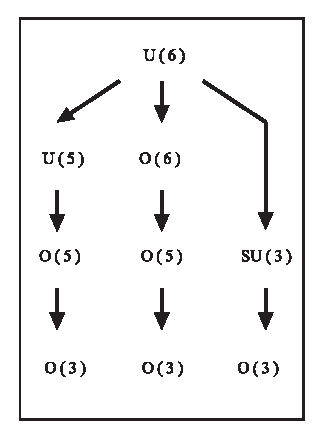
\includegraphics[scale=.65]{figure}
%
% If not, use
%\picplace{5cm}{2cm} % Give the correct figure height and width in cm
%
\caption{Please write your figure caption here}
\label{fig:A1}       % Give a unique label
\end{figure}

% For tables use
%
\begin{table}
\caption{Please write your table caption here}
\label{tab:A1}       % Give a unique label
%
% For LaTeX tables use
%
\begin{tabular}{p{2cm}p{2.4cm}p{2cm}p{4.9cm}}
\hline\noalign{\smallskip}
Classes & Subclass & Length & Action Mechanism  \\
\noalign{\smallskip}\hline\noalign{\smallskip}
Translation & mRNA$^a$  & 22 (19--25) & Translation repression, mRNA cleavage\\
Translation & mRNA cleavage & 21 & mRNA cleavage\\
Translation & mRNA  & 21--22 & mRNA cleavage\\
Translation & mRNA  & 24--26 & Histone and DNA Modification\\
\noalign{\smallskip}\hline\noalign{\smallskip}
\end{tabular}
$^a$ Table foot note (with superscript)
\end{table}
%


\backmatter%%%%%%%%%%%%%%%%%%%%%%%%%%%%%%%%%%%%%%%%%%%%%%%%%%%%%%%
%%%%%%%%%%%%%%%%%%%%%%acronym.tex%%%%%%%%%%%%%%%%%%%%%%%%%%%%%%%%%%%%%%%%%
% sample list of acronyms
%
% Use this file as a template for your own input.
%
%%%%%%%%%%%%%%%%%%%%%%%% Springer %%%%%%%%%%%%%%%%%%%%%%%%%%

\Extrachap{Glossary}


Use the template \emph{glossary.tex} together with the Springer document class SVMono (monograph-type books) or SVMult (edited books) to style your glossary\index{glossary} in the Springer layout.


\runinhead{glossary term} Write here the description of the glossary term. Write here the description of the glossary term. Write here the description of the glossary term.

\runinhead{glossary term} Write here the description of the glossary term. Write here the description of the glossary term. Write here the description of the glossary term.

\runinhead{glossary term} Write here the description of the glossary term. Write here the description of the glossary term. Write here the description of the glossary term.

\runinhead{glossary term} Write here the description of the glossary term. Write here the description of the glossary term. Write here the description of the glossary term.

\runinhead{glossary term} Write here the description of the glossary term. Write here the description of the glossary term. Write here the description of the glossary term.

\Extrachap{Solutions}

\section*{Problems of Chapter~\ref{intro}}

\begin{sol}{prob1}
The solution\index{problems}\index{solutions} is revealed here.
\end{sol}


\begin{sol}{prob2}
\textbf{Problem Heading}\\
(a) The solution of first part is revealed here.\\
(b) The solution of second part is revealed here.
\end{sol}


\printindex

%%%%%%%%%%%%%%%%%%%%%%%%%%%%%%%%%%%%%%%%%%%%%%%%%%%%%%%%%%%%%%%%%%%%%%

\end{document}


import time as tm

begintime = tm.time()

endtime = tm.time()
print('Elapsed time = ', endtime - begintime)

929-249-4000
